\documentclass[10pt]{amsart}
\usepackage[a4paper,margin=23mm]{geometry}
\usepackage{amsmath,amssymb,amsthm,mathtools,hyperref,graphicx,xspace,letltxmacro,xpatch}
\usepackage[english]{babel}
\newtheorem{theo}{Theorem}[section]
\newtheorem{lemm}[theo]{Lemma}\newtheorem{prop}[theo]{Proposition}\newtheorem{coro}[theo]{Corollary}\newtheorem{conj}[theo]{Conjecture}
\theoremstyle{definition}\newtheorem{defi}[theo]{Definition}\newtheorem{rema}[theo]{Remark}\newtheorem{exam}[theo]{Example}\newtheorem{exem}[theo]{Example}\newtheorem{nota}[theo]{Notation}
\newcommand{\ie}{i.e.}\newcommand{\eg}{e.g.}\newcommand{\resp}{resp.}\newcommand{\skpt}{\par\smallskip\noindent}
\emergencystretch=3em\pagestyle{plain}
%~Mouliné par MaN_auto v.0.27.3 2023-04-03 15:40:47

\usepackage{tikz}
\usepackage{tcolorbox}
\usepackage{wasysym}
\usepackage{mathrsfs}
\usepackage{amscd}
\usepackage{subfigure}



\tcbuselibrary{most}
\tcbuselibrary{breakable}


\newtcolorbox{cBoxA}[1][]{enhanced, frame style={purple!80}, interior style={red!0}, #1, }

\newtcolorbox{cBoxB}[2][]{enhanced, frame style={teal!80}, interior style={cyan!0}, #2, }


%\global\long
\newcommand*\eq[1]{\underset{(#1)}{=}}
%\global\long
\newcommand*\ineq[1]{\underset{(#1)}{\leq}}
%\global\long
\newcommand*\ineqs[1]{\underset{(#1)}{\geq}}


%%%%math%%%
\newcommand{\clV}{\mathcal{V}}
\newcommand{\clA}{\mathcal{A}}
\newcommand{\clS}{\mathcal{S}}
\newcommand{\clT}{\mathcal{T}}
\newcommand{\clH}{\mathcal{H}}
\newcommand{\clL}{\mathcal{L}}
\newcommand{\clD}{\mathcal{D}}
\newcommand{\clN}{\mathcal{N}}
\newcommand{\clF}{\mathcal{F}}
\newcommand{\clM}{\mathcal{M}}
\newcommand{\clB}{\mathcal{B}}
\newcommand{\clK}{\mathcal{K}}
\newcommand{\clP}{\mathcal{P}}
\newcommand{\clE}{\mathcal{E}}
\newcommand{\dist}{\mathrm{dist}}
\newcommand{\Ree}{\mathrm{Re}}
\newcommand{\Imm}{\mathrm{Im}}
\newcommand{\divv}{\mathrm{div}}
\newcommand{\Gibbs}{\mathrm{Gibbs}}
\newcommand{\Voll}{\mathrm{Vol}}
\newcommand{\Kerr}{\mathrm{Ker}}
\newcommand{\supp}{\mathrm{supp}}
\newcommand{\Lebb}{\mathrm{Leb}}
\newcommand{\Cste}{\mathrm{Cste}}
\newcommand{\Diag}{\mathrm{Diag}}
\newcommand{\Opp}{\mathrm{Op}}
\newcommand{\Id}{\mathrm{Id}}
\newcommand{\Tr}{\mathrm{Tr}}
\newcommand{\locc}{\mathrm{loc}}
\newcommand{\nonlin}{\mathrm{non-lin}}
\newcommand{\esss}{\mathrm{ess.}}
\newcommand{\bbR}{\mathbb{R}}
\newcommand{\bbC}{\mathbb{C}}
\newcommand{\bbZ}{\mathbb{Z}}
\newcommand{\bbB}{\mathbb{B}}
\newcommand{\bbD}{\mathbb{D}}
\newcommand{\bbN}{\mathbb{N}}
\newcommand{\bbP}{\mathbb{P}}
\newcommand{\bbRP}{\mathbb{RP}}
\newcommand{\scrA}{\mathscr{A}}
\newcommand{\bfC}{\mathbf{C}}

%%%%%%%%%%%%%%%%%%%%%%%%%%%%%%%%%%%%%%%%%%%%%%%%%%%%%%%%%%%%%%%%%%%%%%%%%%%%%%%%%%%%%%%%%%%%%
\makeatletter
\def\editors#1{%
\def\editor@name{#1}
\if@francais
\def\editor@string{Recommand\'e par les \'editeurs \editor@name.}
\else
\def\editor@string{Recommended by Editors \editor@name.}
\fi}
\makeatother

\graphicspath{{./figures/}}

\newcommand*{\mk}{\mkern -1mu}
\newcommand*{\Mk}{\mkern -2mu}
\newcommand*{\mK}{\mkern 1mu}
\newcommand*{\MK}{\mkern 2mu}

%\hypersetup{urlcolor=purple, linkcolor=blue, citecolor=red}

\newcommand*{\romanenumi}{\renewcommand*{\theenumi}{\roman{enumi}}}
\newcommand*{\Romanenumi}{\renewcommand*{\theenumi}{\Roman{enumi}}}
\newcommand*{\alphenumi}{\renewcommand*{\theenumi}{\alph{enumi}}}
\newcommand*{\Alphenumi}{\renewcommand*{\theenumi}{\Alph{enumi}}}
\let\oldtilde\tilde
\renewcommand*{\tilde}[1]{\mathchoice{\widetilde{#1}}{\widetilde{#1}}{\oldtilde{#1}}{\oldtilde{#1}}}
\let\oldexists\exists
\renewcommand*{\exists}{\mathrel{\oldexists}}
\let\oldforall\forall
\renewcommand*{\forall}{\mathrel{\oldforall}}
%%%%%%%%%%%%%%%%%%%%%%%%%%%%%%%%%%%%%%%%%%%%%%%%%%%%%%%%%%%%%%%%%%%%%%%%%%%%%%%%%%%%%%%

\newtheorem{lem}[theo]{Lemma}\newtheorem{rem}[theo]{Remark}
\title{Fractal Weyl upper density bound for smooth Anosov-flow Ruelle spectra}
\author{Faure, Frédéric, Tsujii, Masato}
\date{doi:10.5802/ahl.167; CC BY 4.0}
\begin{document}
\maketitle
\noindent\textit{Editorial note.} Complete original mathematical body and original publisher bibliography retained. Eighteen native rendered vector figure Forms recovered, including original diagram labels; nested component Forms retained in source cache. Cited prior results kept as prerequisites.\par\medskip
\noindent\textit{Allowed standard prerequisites (editorial).}\begin{itemize}
\item Standard functional analysis, measure theory and the author-cited classical theorems. Standard prior results stay cited; complete source-local proofs and definitions retained.
\end{itemize}\medskip
\setcounter{tocdepth}{2}
\tableofcontents{}

%\newpage{}
\begin{rema}
On this pdf file, you can click on the colored words, they contain a hyper-link to \href{https://en.wikipedia.org/wiki/Main_Page}{wikipedia} or other multimedia contents.
\end{rema}



\section{Introduction}

\subsection*{Anosov flow and transfer operator}

In this paper we consider an Anosov flow $\phi^{t}$ on a compact smooth manifold $M$ generated by a smooth vector field $X$. An Anosov flow exhibits sensitivity to initial conditions (or hyperbolicity) and manifests deterministic chaotic behavior. In the 1970's, Rufus Bowen, David Ruelle and Yakov Sinai have constructed the ergodic theory of hyperbolic dynamical systems succeeding the pioneering works of Smale and Anosov. In particular, a functional and spectral approach has been pursued by David Ruelle. This approach consists in describing the evolution, not of individual trajectories which appear unpredictable, but the evolution of functions $u\in C^{\infty}(M)$ under the \emph{transfer operator}
\[
\clL^{t}:u\mapsto e^{\int_{0}^{t}V\circ\phi^{-s}ds}\cdot u\circ\phi^{-t}
\]
where $V\in C^{\infty}(M)$ is a potential function that changes the amplitude along the transport (i.e. push forward) of $u$. This evolution of functions appears to be predictable. In particular it converges towards an equilibrium state in the space of distributions. This approach has progressed from the 70's. It has been shown~\cite{Baladi05,liverani_02,liverani_butterley_07,baladi_05,dyatlov_guillarmou_2014,fred-RP-06,fred-roy-sjostrand-07,fred_flow_09,liverani_04}, that the generator $A=-X+V$ of the evolution operator $\clL^{t}=e^{tA}$ has a discrete spectrum, eigenvalues are called\emph{ Ruelle resonances}, which describes the effective convergence and fluctuations towards the equilibrium state.

\subsection*{Semi-classical analysis with wave packets}

Due to hyperbolicity of the Anosov flow, the transfer operator $\clL^{t}$ sends the\linebreak information towards small scales and technically it is natural to use semi-classical analysis which concerns the large frequency components of distributions. Following the idea of semi-classical analysis, we consider the flow $\phi^{t}$ lifted to the cotangent space $\tilde{\phi}^{t}=(d\phi^{-t})^{*}:T^{*}M\rightarrow T^{*}M$ that encodes both the localization of a function and its internal frequency. This lifted flow $\tilde{\phi}^{t}$ is a Hamiltonian flow and preserves the level sets of the frequency along the flow direction which are co-dimension one affine sub-bundles of $T^{*}M$. The assumption of hyperbolicity implies that $\tilde{\phi}^{t}$ restricted to such a sub-bundle has a compact trapped set (or, non-wandering set) and that the dynamics scatters on this trapped set~\cite{fred-roy-sjostrand-07,fred_flow_09}. The existence and properties of the discrete Ruelle spectrum follows from this observation and the uncertainty principle (i.e. effective discreteness of $T^{*}M$ into symplectic boxes) and rejoins a more general theory of semi-classical analysis developed in the 1980's by B. Helffer and J.~Sj\"ostrand called quantum scattering on phase space~\cite{sjostrand_87}.

In the papers~\cite{fred-roy-sjostrand-07,fred_flow_09}, the semi-classical analysis is performed with the H\"ormander's theory of pseudo-differential operators, considering the generator\linebreak $A=-X+V$ of the transfer operator $\clL^{t}=e^{tA}$. In this paper we adopt a slightly different approach: in Section~\ref{sec:Semiclassical-analysis-with}, we develop an analysis using wave packets $\Phi_{\rho}$ that are parameterized by points $\rho\in T^{*}M$ on the cotangent space. The precise structure of these wave packet is determined by a metric $g$ on $T^{*}M$ that is compatible with the symplectic structure and adapted to the dynamics. In other words the metric measures the uncertainty principle. From these wave packets we define a wave-packet transform $\clT :C^{\infty}(M)\rightarrow\clS(T^{*}M)$ by $(\clT u)(\rho)=\langle\Phi_{\rho}|u\rangle_{L^{2}(M)}$. Then the semi-classical analysis is performed on $T^{*}M$, considering the transfer operator $\clL^{t}$ for some range of time $t\in[0,T]$ and analyzing the Schwartz kernel of the equivalent lifted operator on phase space $T^{*}M$ given by $\tilde{\clL}_{W}^{t}:=W\clT\clL^{t}\clT^{\dagger}W^{-1}$, conjugated by some suitable weight $W$. From this analysis we deduce properties of the resolvent operator $(z-A)^{-1}$ and then properties of the spectrum of the generator $A$.

This approach using phase space representation with wave-packet transform $\clT$\footnote{The wave packet transform that we consider in this paper is related to Anti-Wick quantization, Berezin quantization, FBI transforms, Bargmann--Segal transforms, Gabor frames and Toeplitz operators~\cite[Chap.~3]{martinez-01}, \cite{wunsh-zworski_01}, \cite[Chap.~13]{zworski_book_2012}, \cite{sjostrand_hitrick_07,sjostrand_density_resonances_96}.} and a metric $g$ on the phase space $T^{*}M$ is similar to the Weyl--H\"ormander calculus~\cite{hormander1979weyl}, \cite[Section~2.2]{lerner2011metrics} and is also similar to the approach taken in~\cite{faure-tsujii_prequantum_maps_12,faure-tsujii_anosov_flows_13,tsujii_08,tsujii_FBI_10} for dynamical systems. It will provide a new proof of Theorem~\ref{thm:Discrete_spectrum} below that shows the existence of a discrete spectrum for $A$ and, further, enables us to give some new results, Theorems~\ref{thm:Weyl law}, \ref{thm:grey-band} and~\ref{thm:WF} in this paper.

Technically one advantage of using micro-local analysis with wave packets\linebreak (i.e. Toeplitz quantization) instead of the more usual Weyl quantization is that it allows to consider symbols on $T^{*}M$ that are not necessarily smooth functions. This is particularly interesting in the context of Anosov flows where the stable/unstable foliations are H\"older continuous. However it may be possible to develop an analysis similar to the one that we develop here, but using Weyl quantization and techniques called ``second micro-localization'' and ``exotic calculus''. We think that another advantage of using the metric $g$ and wave-packets quantization is to provide a better geometric insight and meaning to these difficult techniques.

One purpose of this paper is to put the basis of this micro-local analysis using wave-packets in preparation for a more refined analysis in case of contact Anosov flows. This second step is done in the more recent paper~\cite{faure-tsujii_anosov_flows_16}.

In a recent paper~\cite{bonthonneau2020fbi} Yannick Guedes Bonthonneau and Malo Jézéquel develop FBI transform in Gevrey classes for Anosov flows in order to analyze the internal Ruelle spectrum. In Gevrey classes, we can use a stronger escape function than in smooth classes and this permits to reveal the whole Ruelle spectrum at once.

\subsection*{Discrete spectrum of the generator}

Using the semi-classical analysis depicted previously, for any $C>0$, we can design a positive function $W$ on $T^{*}M$ and some \emph{anisotropic Sobolev space} $\clH _{W}$ in which the transfer operator $\clL^{t}$ acts as a strongly continuous semi-group and its generator $A=-X+V$ has discrete spectrum on the spectral domain $\Ree(z)>-C$~\cite{liverani_butterley_07,fred_flow_09}. This discrete spectrum is intrinsic to the flow, i.e. does not depend on the choice of the space $\clH _{W}$ (but of course the norm of the resolvent depends on $\clH _{W}$). In this paper our semi-classical approach using wave packets permits to design anisotropic Sobolev spaces $\clH _{W}$ with more accurate properties than previously constructed ones~\cite{fred_flow_09} and this leads to new refined results on the Ruelle spectrum. For example we show in Theorem~\ref{thm:grey-band} that $\clL^{t}$ for $t\in\bbR$ form a strongly continuous group on $\clH _{W}$ and not only a semi-group. We also obtain refined estimate on the density of the eigenvalues in Theorem~\ref{thm:Weyl law} and more precise description of the eigendistributions in terms of their wave front set in Theorem~\ref{thm:WF}.

The general ideas that sustain the analysis performed in this paper, Theorem~\ref{thm:Discrete_spectrum} on the discrete spectrum and related properties, are summarized as follows:
\begin{enumerate}
\item Any distribution in $\clD'(M)$ can be decomposed as a superposition of wave-packets $\Phi_{\rho}$ parameterized by $\rho\in T^{*}M$ on cotangent space. This family of wave-packets is determined by an admissible metric $g$ on $T^{*}M$, which is compatible with the symplectic form asymptotically flat and also adapted to the lifted dynamics on $T^{*}M$. We define and use the wave-packet transform\linebreak $\clT:C^{\infty}(M)\rightarrow\clS(T^{*}M)$ which expresses a function in $C^{\infty}(M)$ as superposition of the wave-packets $\Phi_{\rho}$ in Section~\ref{subsec:Resolution-of-identity}.
\item The transfer operator $\clL^{t}$ transforms a wave packet $\Phi_{\rho}$, $\rho\in T^{*}M$, into another (deformed) wave packet at position $\tilde{\phi}^{t}(\rho)\in T^{*}M$ where $\tilde{\phi}^{t}:T^{*}M\rightarrow T^{*}M$ is the canonical lift of the flow $\phi^{t}$. Precisely the Schwartz kernel of the lifted operator $\clT\clL^{t}\clT^{\dagger}:\clS(T^{*}M)\rightarrow\clS(T^{*}M)$ decays very fast on the outside of the graph of $\tilde{\phi}^{t}$. In other terms, $\clL^{t}$ is a Fourier integral operator whose associated canonical map is $\tilde{\phi}^{t}$. This property is expressed in Theorem~\ref{thm:Microlocality-of-the_TO} usually called ``propagation of singularities''.
\item For an Anosov flow $\phi^{t}$, the trajectories of the lifted flow $\tilde{\phi}^{t}$ in $T^{*}M$ escape to infinity for $t\mapsto+\infty$ or $t\rightarrow-\infty$, except for points on a trapped set (or non-wandering set), which is compact for each frequency $\omega$ along the flow direction. See Figure~\ref{fig:The-Anosov-flow-on_T*M}. One can then find an admissible positive escape function (or Lyapunov function) $W$ on $T^{*}M$ that is ``temperate and moderately varying with respect to the metric $g$'' and decreases exponentially along the flow $\tilde{\phi}^{t}$ on the outside of the trapped set. By considering $W$ as a $L^{2}-$weight on $T^{*}M$, we define the anisotropic Sobolev space $\clH _{W}(M)$ and show that the generator $A:\clH _{W}(M)\rightarrow\clH _{W}(M)$ has a discrete spectrum. Appendix~\ref{sec:A-simple-model-of resonances} illustrates the choice of $W$ and the appearance of discrete spectrum in $\clH _{W}$ with a very simple matrix model.
\end{enumerate}

\section{Results}\label{sec:Results}

In this section we present the main results that we obtain in this paper concerning the Ruelle spectrum of Anosov flows.

We first review the following theorem that defines the discrete spectrum of Ruelle resonances. We write $\clD'(M)$ for the space of distributions on $M$ and $H^{r}(M)\subset\clD'(M)$ for the Sobolev space of order $r\in\bbR$. We refer to~\cite[Defi.~2.1 page 4]{pazy_semigroups_83}, \cite[p.~79]{engel_1999} for generalities about semi-groups of operators. $\lambda_{\min}>0$ is the exponent of hyperbolicity defined in~\eqref{eq:hyperbolicity}.

\begin{cBoxB}{}
\begin{theo}[{Discrete spectrum~\cite{liverani_butterley_07,fred_flow_09}}]\label{thm:Discrete_spectrum}
Let $X$ be a smooth Anosov vector field on a closed manifold $M$ (considered as a differential operator). Let $V\in C^{\infty}(M;\bbC)$ be a smooth function and let $A:=-X+V$. For any $r\geq0$ there exists a Hilbert space $\clH _{W}(M)$, called an anisotropic Sobolev space, satisfying
\begin{equation}\label{eq:H_W}
H^{r}\left(M\right)\subset\clH _{W}\left(M\right)\subset H^{-r}\left(M\right)
\end{equation}
such that the transfer operator $\clL^{t}=\exp(tA)$ for $t\geq0$ extends to a \emph{strongly continuous semi-group} on $\clH _{W}(M)$. The generator $A$ has discrete spectrum (discrete eigenvalues with finite multiplicities) on the spectral domain $D_{W}=\{ z\in\bbC\mid\Ree(z)>C_{X,V}-r\lambda_{\min}\} $, with $C_{X,V}\in\bbR$ given in~\eqref{eq:C_XV}. These discrete eigenvalues are called \emph{Ruelle resonances}. The Ruelle resonances and the corresponding generalized eigenspaces are intrinsic, i.e. they do not depend on the choice of the space $\clH _{W}(M)$, see~\cite[Theorem~1.5]{fred_flow_09} or~\cite[Lemma~B.3]{jezequel2020spectral_thesis}. See Figure~\ref{fig:discrete_spectrum}$\MK$(a).
\end{theo}
\end{cBoxB}

Theorem~\ref{thm:Discrete_spectrum}, giving discrete spectrum for Anosov flows, has been obtained first by O. Butterley and C. Liverani (for some Banach spaces) in~\cite{liverani_butterley_07}. A proof using semi-classical analysis and anisotropic Sobolev spaces has been obtained in~\cite{fred_flow_09}. A generalization to Axiom A flows (and some open uniformly hyperbolic dynamics) has been obtained in~\cite{dyatlov_guillarmou_2014, https://doi.org/10.48550/arxiv.2107.08875}.

\begin{rema}
Notice that in Theorem~\ref{thm:Discrete_spectrum}, the set of operators $\clL^{t}=\exp(tA)$ for $t\geq0$ in $\clH _{W}(M)$ form a semi-group and not a group. Indeed, in the space $\clH _{W}(M)$ proposed in the papers~\cite{liverani_butterley_07,fred_flow_09}, the operator $\clL^{t}$ is not invertible. For negative time, we need to construct a different space to get a semi-group. In this paper, we somehow improve this aspect, in Theorem~\ref{thm:grey-band} below, where we propose a space $\clH _{W}(M)$ in which the set of operators $\clL^{t}=\exp(tA)$ for $t\in\bbR$ form a group. This group property (that provides invertibility) has been used for example in~\cite{faure-tsujii_anosov_flows_16}.
\end{rema}


\subsection{Upper bound for density of eigenvalues}
%\begin{flushleft}
In the next theorem we obtain an upper bound for the density of resonances in the limit of high frequencies $\omega=\Imm(z)$. This bound depends on the H\"older exponent $0<\beta_{0}\leq1$ of the distribution $E_{u}\oplus E_{s}$ (strong stable and unstable) defined in~\eqref{eq:Holder_exp}. Recall that $n=\dim M-1$. For $s\in\bbR$, we set
\begin{equation}\label{eq:def_Japonese_bracket}
\langle s\rangle:=\left(1+s^{2}\right)^{1/2}\underset{\left|s\right|\gg1}{\sim}\left|s\right|.
\end{equation}
%\end{flushleft}

%%%%%%%%%%%%%%%%%%%%%%%%%%%
%\begin{cBoxB}{}
\begin{tcolorbox}[enhanced, frame style={teal!80}, interior style={cyan!0},breakable]

\begin{theo}[Fractal Weyl law: upper bound for density of eigenvalues]\label{thm:Weyl law}\ \\*[-0.10em]
%\begin{flushleft}
Let $X$ be a smooth Anosov vector field on a closed manifold $M$ and $V\in C^{\infty}(M;\bbC)$. Let $\sigma_{+}(A)\subset\bbC$ be the discrete Ruelle spectrum defined in Theorem~\ref{thm:Discrete_spectrum} for the operator $A=-X+V$. Then, for any $\gamma\in\bbR$, there exists $C>0$ such that
\begin{multline}\label{eq:weyl_upper_bound}
\sharp\left\{ z\in\sigma_{+}\left(A\right);\quad\Ree\left(z\right)>\gamma,\,\Imm\left(z\right)\in\left[\omega,\omega+1\right]\right\}\\ \leq C\left\langle \omega\right\rangle ^{\frac{n}{1+\beta_{0}}} \quad\text{for any}\:\omega\in\bbR.
\end{multline}
%\end{flushleft}
\end{theo}

\end{tcolorbox}
%\end{cBoxB}
%%%%%%%%%%%%%%%%%%%%%%%%%%%

The proof of Theorem~\ref{thm:Weyl law} is given in Section~\ref{subsec:Dynamics-lifted-in} and relies on an adapted phase space metric $g$ and escape function $W$ (that defines the Hilbert space $\clH _{W}(M)$) to the non-smooth trapped set. Note that the exponent $\frac{n}{1+\beta_{0}}$ in the upper bound~\eqref{eq:weyl_upper_bound} depends on the H\"older exponent $0<\beta_{0}<1$ in~\eqref{eq:Holder_exp}. This kind of upper bound has been called fractal Weyl law after the work of J. Sj\"ostrand\cite{sjostrand_90}, see also~\cite{Nonnenmacher_Zworski_14}.

Concerning the upper bound~\eqref{eq:weyl_upper_bound}, there are a few preceding results:
\begin{itemize}
\item For general Anosov flows, i.e. without assumption on $\beta_{0}$, in~\cite[Theorem~1.8]{fred_flow_09}, the density upper bound $o(\langle \omega\rangle ^{n})$ has been obtained for intervals in $\Imm(z)$ of width $\langle \omega\rangle ^{\frac{1}{2}}$.
\item Under the assumption that $m\mapsto E_{u}(m)\oplus E_{s}(m)$ is smooth (and therefore $\beta_{0}=1$), in~\cite{dyatlov_Ruelle_resonances_2012}, the density upper bound \emph{$O(\langle \omega\rangle ^{\frac{n}{2}})$} is obtained.
\item For contact Anosov flows (where $E_{u}\oplus E_{s}$ is smooth and $\beta_{0}=1$), in~\cite{faure_tsujii_band_CRAS_2013,faure-tsujii_anosov_flows_13,faure-tsujii_anosov_flows_16}, we obtained the density lower bound $C^{-1}\langle \omega\rangle ^{\frac{n}{2}}$ under some conditions that guarantee the band structure of the spectrum. In a more recent work~\cite{faure-tsujii_anosov_flows_16} we obtain the precise asymptotic expression for the density under some pinching conditions.
\end{itemize}

\subsubsection{\label{subsec:Heuristic-explanation-of}
Heuristic explanation of the fractal exponent \texorpdfstring{$\frac{n}{1+\beta_{0}}$}{n/1+ beta0}}

The presence of $\beta_{0}$ in the denominator of the exponent $\frac{n}{1+\beta_{0}}$ in~\eqref{eq:weyl_upper_bound} may look strange at first sight since a usual treatment of the upper bound in the Weyl law considers minimal coverings of the trapped set by boxes of size $\delta x=\omega^{-1/2}$, $\delta\xi=\omega^{1/2}$ for large $\omega\gg1$ and, as explained below, would give the weaker upper bound 
\[
O\left(\omega^{\frac{\dim_{B}\scrA-1}{2}}\right)=O\left(\omega^{n\left(1-\frac{\beta_{0}}{2}\right)}\right)\quad\text{where}\quad\dim_{B}\scrA=\underbrace{(n+1)}_{\dim M}+n(1-\beta_{0})
\]
is the fractal box dimension of the graph of the Anosov one form $\scrA$, Eq.\eqref{eq:one_form}, see~\cite[Chap.~11]{falconer_03_book}, \cite{Nonnenmacher_Zworski_14}. To obtain the better bound $O(\omega^{\frac{n}{1+\beta_{0}}})$, we consider coverings by boxes of size $\delta x=\omega^{-\alpha}$, $\delta\xi=\omega^{\alpha}$ where $\frac{1}{2}\leq\alpha<1$ is an arbitrary parameter (that enters in the metric~\eqref{eq:metric_g_in_coordinates} under the name $\alpha^{\perp}$) and we set $\alpha=\frac{1}{\beta_{0}+1}$ at the end in order to optimize the result. Below we explain this argument in more detail.

We consider some fixed frequency $\omega$ along the flow and assume that $\omega$ is large. We will see\footnote{In flow box coordinates we have $-X=\frac{\partial}{\partial z}$, hence a function that has frequency $\omega$ along the flow writes $u(x,z)=u_{0}(x)e^{i\omega z}$ giving $-Xu=i\omega u$.} that it corresponds with $\omega=\Imm(z)$ on the spectral domain. It will appear in the proof that, after damped by a weight function $W$ on $T^{*}M$, Ruelle eigenfunctions at frequency $\omega$ are micro-locally supported in a vicinity of the graph of the map $m\in M\mapsto\omega\scrA(m)\in T^{*}M$ where $\scrA$ is the Anosov one form~\eqref{eq:one_form}. We call this graph the \emph{trapped set}. In general it is a fractal set~\cite[Chap.11]{falconer_03_book} because $\scrA$ is not smooth. See Figure~\ref{fig:fractal_bound}. In order to describe all the set of resonant states (or eigenfunctions) near frequency $\omega$, we consider a covering of this graph by symplectic boxes\footnote{In coordinates $(y_{j})_{j}$ on $M$ and dual coordinates $(\eta_{j})_{j}$ on $T_{y}^{*}M$, a symplectic box in $T^{*}M$ has size $\Delta y^{j}=\delta$ and $\Delta\eta_{j}=\delta^{-1}$ for some $\delta>0$, hence symplectic volume~1.} of unit size (corresponding to wave packets) and count how many boxes $\clN(\omega)$ we need. This number of boxes $\clN(\omega)$ will give an upper bound for the number of eigenvalues. Assume that each symplectic box has size $\delta x\sim\omega^{-\alpha}$ on the manifold $M$, transversely to the flow, with some exponent $\frac{1}{2}\leq\alpha<1$. The symplectic condition (or uncertainty principle) imposes $\delta x.\delta\xi=1$, i.e. the size $\delta\xi\sim\delta x^{-1}\sim\omega^{\alpha}$ in the fibers of $T^{*}M$ transversely to the trapped set $\bbR\scrA$, as on Figure~\ref{fig:Unity_ball}. Due to its H\"older exponent $\beta_{0}$, the graph of $\omega\scrA$ spreads over a range of frequencies of size {\small{}$\delta(\omega\scrA)\sim\omega(\delta x)^{\beta_{0}}=\omega^{1-\alpha\beta_{0}}$}. Then there are two cases to consider, see Figure~\ref{fig:fractal_bound}:
\begin{enumerate}
\item If $\alpha\leq\frac{1}{1+\beta_{0}}\Leftrightarrow1-\alpha\beta_{0}\geq\alpha$, then for large frequencies $\omega$, we have $\omega^{1-\alpha\beta_{0}}\geq\omega^{\alpha}\Leftrightarrow\delta(\omega\clA)\geq\delta\xi$, i.e. the variance $\delta(\omega\clA)$ of $\omega\clA$ is larger than the size $\delta\xi$ of the box in the frequency space. The symplectic volume to be covered by the boxes will be proportional to $(\delta(\omega\clA))^{n}$. This gives the estimate $\clN(\omega)\asymp(\delta(\omega\clA))^{n}=\omega^{n(1-\beta_{0}\alpha)}$.
\item On the contrary, if $\alpha\geq\frac{1}{1+\beta_{0}}$, the variance $\delta(\omega\clA)$ of $\omega\clA$ is smaller than the size $\delta\xi$ of the box in the frequency space. In this case, the symplectic volume to be covered by the boxes will be proportional to $(\delta\xi)^{n}$. This gives the estimate $\clN(\omega)\asymp(\delta\xi)^{n}=\omega^{n\alpha}$.
\end{enumerate}
The value of $\alpha$ that minimizes $\clN(\omega)$ is $\alpha=\frac{1}{1+\beta_{0}}$, giving $\clN(\omega)\asymp\omega^{\frac{n}{1+\beta_{0}}}$, that is the upper bound~\eqref{eq:weyl_upper_bound} in Theorem~\ref{thm:Weyl law}.

%{\footnotesize{}}
\begin{figure}[!htbp]
\centering
\begin{subfigure}
{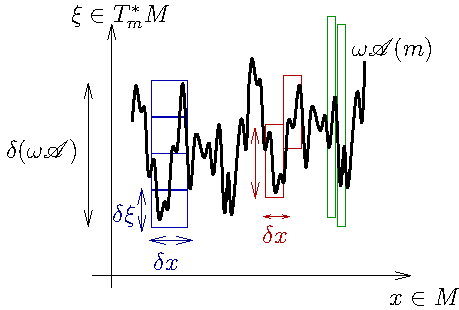
\includegraphics[scale=0.9]{figures/fractal_bound-1.pdf}}
\end{subfigure}
\hfill
\begin{subfigure}
{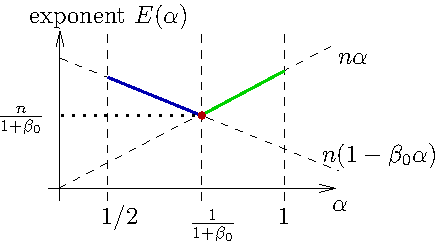
\includegraphics[scale=0.9]{figures/exponent_alpha-1.pdf}}
\end{subfigure}
\caption{To estimate from above the density of resonances at frequency $\omega$, we cover the trapped set, i.e. the graph of the map $m=(x,z)\in M\protect\mapsto\omega\scrA(m)\in T^{*}M$ by symplectic boxes, where $x$ is a coordinate transverse to the flow direction. This graph is H\"older continuous with exponent $\beta_{0}$. With the choice $\delta x=\omega^{-\alpha}$ we obtain that the symplectic volume of this cover is $\omega^{E(\alpha)}$ with some exponent $E(\alpha)$ that is minimum for the choice $\alpha=\frac{1}{1+\beta_{0}}$. On the picture, the cover in the middle (red boxes) is more efficient than the left one (blue boxes) or the right one (green boxes).}
\label{fig:fractal_bound}
\end{figure}

\subsection{Parabolic wave front set of the Ruelle eigenfunctions}

Concerning the eigendistributions associated to the Ruelle spectrum, we obtain in Theorem~\ref{thm:WF} and Corollary~\ref{cor:Let-us-choose} below a precise description of their semi-classical wave front set, that is, the region in the phase space $T^{*}M$ where the Ruelle eigenfunctions are non negligible. In these results, the wave front sets are contained in a parabolic vicinity of the unstable affine distribution $E_{u}^{*}+\omega\clA$ uniformly in $\omega$ (where $\clA\in(E_{u}\oplus E_{s})^{\perp}$ is the Anosov one form and $\omega$ is the imaginary part of the corresponding eigenvalue) and this improves the previous results~\cite{fred_flow_09} which claims that the wave front set is contained in an arbitrary conical vicinity of $E_{u}^{*}$. See Figure~\ref{fig:Wave-front-set} that compares these two results.

We will use the decomposition of $T^{*}M=E_{u}^{*}\oplus E_{s}^{*}\oplus E_{0}^{*}$ dual to~\eqref{eq:decomp_TM}, where
\[
E_{u}^{*}=\left(E_{u}\oplus E_{0}\right)^{\perp},\quad E_{s}^{*}=\left(E_{s}\oplus E_{0}\right)^{\perp},\quad E_{0}^{*}=\left(E_{u}\oplus E_{s}\right)^{\perp}.
\]
We first recall the definition of the wave front set $WF(u)$ of a distribution $u\in\clD'(M)$ from~\cite[p.~254]{hormander_1},\cite[p.~77]{grigis_sjostrand},\cite[p.~27]{taylor_tome2}. A point $(m,\eta)\in T^{*}M$ does not belong to $WF(u)$ if and only if there exist a smooth function $\chi\in C^{\infty}(M;\bbR^{+})$ with $\chi(m)=1$ and an open cone $\bfC\subset\bbR^{n+1}$ with $\eta\in\bfC$ such that, for any $N>1$, we have
\[
\left|\left(\clF\left(\chi u\right)\right)\left(\eta'\right)\right|\leq\frac{C_{N}}{\left|\eta'\right|^{N}}\quad\text{for all }\eta'\in\bfC,
\]
with some constant $C_{N}$, where $\clF$ is the Fourier transform (in a local chart).

The following theorem describes what is known from~\cite{fred_flow_09} concerning the wave front set $WF(u)$ of a Ruelle generalized eigenfunction\footnote{A generalized eigenfunction of a linear operator $A$ for an eigenvalue $z\in\bbC$ is a distribution $u\in\clD'(M)$ such that $(z-A)^{n}u=0$ for some $n\geq1$.}.

\begin{cBoxB}{}
\begin{theo}[Conical wave front set]\label{thm:conical-WF}
\cite{fred_flow_09} Assume that $u\in\clH _{W}(M)$ is a generalized eigenfunction of the generator $A$ for a Ruelle eigenvalue $z\in\bbC$. Then we have
\[
WF\left(u\right)\subset E_{u}^{*}=\left(E_{u}\oplus E_{0}\right)^{\perp}.
\]
\end{theo}
\end{cBoxB}

The claim of Theorem~\ref{thm:conical-WF} is illustrated on Figure~\ref{fig:Wave-front-set}$\MK$(a). In Theorem~\ref{thm:WF} below, we give a more precise description of the singularities of Ruelle eigenfunctions. For this, we first introduce (a simplified version of) the wave packet transform.

\begin{figure}[!htbp]
\centering
%\includegraphics[scale=0.90]{figures/WF-1.pdf} 
\begin{subfigure}[]
{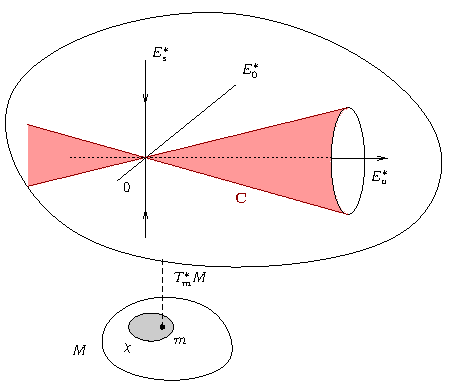
\includegraphics[scale=1.30]{WF-1-a-1.pdf}}
\end{subfigure}
\vspace*{-10pt}
\begin{subfigure}[]
{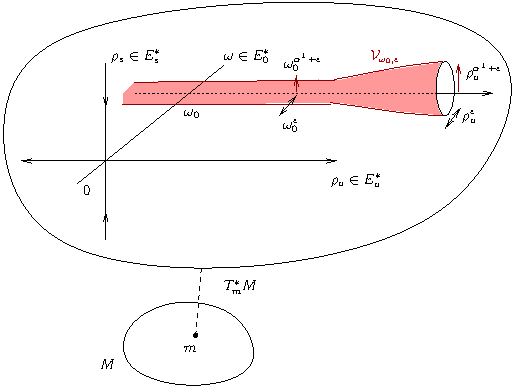
\includegraphics[scale=1.30]{WF-1-b-1.pdf}}
\end{subfigure}
%\figure/WF.pdftex_t}}
\caption{\label{fig:Wave-front-set}
\textbf{(a)} Theorem~\ref{thm:conical-WF} shows that for high frequencies a Ruelle eigendistribution represented in phase space $T^{*}M$ is negligible outside any conical vicinity of the linear sub-bundle $E_{u}^{*}\subset T^{*}M$.\textbf{ (b)} Theorem~\ref{thm:WF} improves this description and shows that a Ruelle eigendistribution with eigenvalue $z=a+i\omega_{0}$, is negligible outside a ``parabolic domain'' \emph{$\clV_{\omega_{0},\epsilon}$} of the affine sub-bundle $\omega_{0}\scrA+E_{u}^{*}\subset T^{*}M$, uniformly with respect to $\omega_{0}\in\bbR$. Here $\alpha^{\perp}=\frac{1}{1+\min(\beta_{u},\beta_{s})}\in[\frac{1}{2};1[$ and $\epsilon>0$ is arbitrary small. Observe that the cone $C$ contains the domain $\clV_{\omega_{0},\epsilon}$, except for a compact part of it.}
\end{figure}


\subsubsection{Metric \texorpdfstring{$g$}{g} on \texorpdfstring{$T^{*}M$}{T*M}}

The analysis made in this paper relies on the use of a specific metric on $T^{*}M$. From this metric $g$ we will define later the wave packet transform. We consider local flow box coordinates $y=(x,z)\in\bbR^{n}\times\bbR$ for the vector field $X$ on an open set $U\subset M$, which is by definition a local chart map $\kappa:m\in U\subset M\mapsto y=(x,z)\in\bbR^{n}\times\bbR$, such that
\begin{equation}\label{eq:X_ddz}
\kappa_{*}\left(-X\right)=\frac{\partial}{\partial z}.
\end{equation}
We write $\eta=(\xi,\omega)\in\bbR^{n}\times\bbR$ for the dual coordinates on $T_{(x,z)}^{*}\bbR^{n+1}\equiv\bbR^{n}\times\bbR$. Let $\tilde{\kappa}:\rho\in T^{*}U\mapsto(y,\eta)\in T^{*}\bbR^{n+1}$ be the canonical extension of the local chart map $\kappa$ to the cotangent bundle.

Let us consider parameters $\alpha^{\perp},\alpha^{\parallel}\in[0,1[$ such that
\begin{equation}\label{eq:conditions}
0\leq\alpha^{\parallel}<\alpha^{\perp}<1,\quad\frac{1}{2}\leq\alpha^{\perp}<1.
\end{equation}
Let
\begin{equation}\label{eq:def_delta}
\delta^{\perp}\left(\eta\right):=\left\langle \left|\eta\right|\right\rangle ^{-\alpha^{\perp}},\quad\delta^{\parallel}\left(\eta\right):=\left\langle \left|\eta\right|\right\rangle ^{-\alpha^{\parallel}},
\end{equation}
where $|\eta|$ denotes the Euclidean norm in $\bbR^{n+1}$ and consider the following metric $g$ on $T^{*}\bbR^{n+1}$ given at each point
\[
\varrho=\left(y,\eta\right)=\left(\left(x,z\right),\left(\xi,\omega\right)\right)\in T^{*}\bbR^{n+1}
\]
by
\begin{equation}\label{eq:metric_g_in_coordinates}
g_{\varrho}:=\left(\frac{dx}{\delta^{\perp}\left(\eta\right)}\right)^{2}+\left(\delta^{\perp}\left(\eta\right)d\xi\right)^{2}+\left(\frac{dz}{\delta^{\parallel}\left(\eta\right)}\right)^{2}+\left(\delta^{\parallel}\left(\eta\right)d\omega\right)^{2}.
\end{equation}
The metric $g$ is compatible\footnote{Indeed we have $g(u,v)=\Omega(u,Jv)$ if we define an almost complex structure $J$ by
\begin{align*}
J\left(\delta^{\perp}\left(\eta\right)\partial_{x}\right) & =\frac{1}{\delta^{\perp}\left(\eta\right)}\partial_{\xi},\quad J\left(\frac{1}{\delta^{\perp}\left(\eta\right)}\partial_{\xi}\right)=-\delta^{\perp}\left(\eta\right)\partial_{x},\\
J\left(\delta^{\parallel}\left(\eta\right)\partial_{z}\right) & =\frac{1}{\delta^{\parallel}\left(\eta\right)}\partial_{\omega},\qquad J\left(\frac{1}{\delta^{\parallel}\left(\eta\right)}\partial_{\omega}\right)=-\delta^{\parallel}\left(\eta\right)\partial_{z}.
\end{align*}
}~\cite{da_silva_01,mac_duff_98} with the canonical symplectic form on $T^{*}M$: $\Omega=\sum_{k=1}^{n+1}dy_{k}\wedge d\eta_{k}$. The norm of a vector $v\in\bbR^{2(n+1)}$ with respect to $g$ is denoted by
\begin{equation}\label{eq:def_norm_g}
\left\Vert v\right\Vert _{g_{\varrho}}:=\left(g_{\varrho}\left(v,v\right)\right)^{1/2}.
\end{equation}
The unit ball for the metric is illustrated on Figure~\ref{fig:Unity_ball}.

As we will see in Section~\ref{subsec:Lipschitz-property-of}, the conditions~\eqref{eq:conditions} ensure that different choices of flow box charts give a uniformly equivalent metric on the intersection and consequently defines an equivalence class of metric on the cotangent bundle $T^{*}M$.

\begin{figure}[h]
\centering
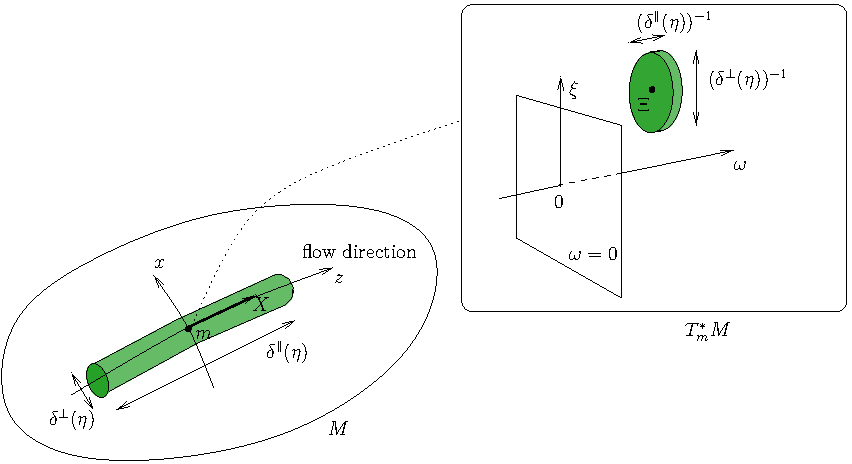
\includegraphics[scale=0.8]{figures/Unity_ball-1.pdf} 
%\scalebox{0.8}[0.8]{\failedinput{figure/Unity_ball.pdftex_t}}
\caption{We use flow box coordinates $y=(x,z)$ on $M$ i.e. such that the vector field is $(-X)=\frac{\partial}{\partial z}$ and dual coordinates $\eta=(\xi,\omega)$ in $T_{m}^{*}M$. $g$ is a (class of) metric on $T^{*}M$ and the filled cylinders (in green) represent the unit ball for this metric $g$ at a point $\rho\in T^{*}M$, projected on the base $M$ and on the fiber $T_{m}^{*}M$ with $m=\pi(\rho)$. This unit ball has size $\delta^{\parallel}(\eta)$ along the flow $z$, transverse size $\delta^{\perp}(\eta)$ along $x$ and sizes $(\delta^{\perp}(\eta))^{-1},(\delta^{\parallel}(\eta))^{-1}$ along dual coordinates $\xi,\omega$ in $T_{m}^{*}M$. These sizes $\delta^{\perp}(\eta)\protect\leq\delta^{\parallel}(\eta)\protect\leq1$ are functions on $T^{*}M$, defined in~\eqref{eq:def_delta}, and decay at infinity.}
\label{fig:Unity_ball}
\end{figure}


\subsubsection{Wave packet transform}

For a given $\varrho=(y,\eta)\in T^{*}\bbR^{n+1}$ we define the Gaussian function $\Phi_{\varrho}\in C_{0}^{\infty}(\bbR^{n+1};\bbC)$ called wave packet:
\begin{equation}\label{eq:wave_packet_1}
\begin{split}
\Phi_{\varrho}\left(y'\right) & =a_{\varrho}\chi\left(y'-y\right)\exp\left(i\eta.y'-\left\Vert y'-y\right\Vert _{g_{\varrho}}^{2}\right)
\\
& =a_{\varrho}\chi\left(y'-y\right)\exp\left(i\eta.y'-\left|\frac{\left(z'-z\right)}{\delta^{\parallel}\left(\eta\right)}\right|^{2}-\left|\frac{\left(x'-x\right)}{\delta^{\perp}\left(\eta\right)}\right|^{2}\right)
\end{split}
\end{equation}
with $y'=(x',z')$ and where $\chi\in C_{0}^{\infty}(\bbR^{n+1})$ is some cut-off function with $\chi\equiv1$ near the origin and $a_{\varrho}>0$ is such that $\Vert
\Phi_{\varrho}\Vert _{L^{2}(\bbR^{n+1})}=1$. We define the wave-packet transform of a distribution $u\in\clD'(M)$ on $T^{*}U$ by\footnote{The wave-packet transform $\clT$ defined here is similar to
\href{https://en.wikipedia.org/wiki/Segal\%E2\%80\%93Bargmann_space}{Bargmann
transform}.}
\begin{equation}
\left(\clT_{g}u\right)\left(\rho\right):=\left\langle\Phi_{\tilde{\kappa}\left(\rho\right)}\circ\kappa\,\middle|\,u\right\rangle_{L^{2}\left(M\right)},\quad\text{with }\rho\in T^{*}U.
\end{equation}

\begin{rema}
Later we will introduce in~\eqref{eq:wave_packet} an expression for wave packets that is slightly different but converges to~\eqref{eq:wave_packet_1} in the high frequency limit. The expression will be more complicated but will have the advantage of giving an exact resolution of identity. Since both expressions become essentially equivalent in the high frequency limits, the definitions and properties given in this section are not affected by the difference.
\end{rema}


\subsubsection{Conical wave front set}

We first reformulate Theorem~\ref{thm:conical-WF} using the wave packet transform $\clT_{g}u$ using the metric $g$ as follows. Assume that $u\in\clH _{W}(M)$ is a generalized eigenfunction of the generator $A$ for a Ruelle eigenvalue $z\in\bbC$ given in Theorem~\ref{thm:grey-band}. Then, for any continuous field of open positive cones $\bfC:m\in M\mapsto\bfC(m)\subset T_{m}^{*}M$ with $\bfC(m)\supset E_{u}^{*}(m)$ and for any $N>1$, there exists $C_{N}>0$ such that
\begin{equation}\label{eq:WF}
\left|\left(\clT_{g}u\right)\left(\rho\right)\right|\leq\frac{C_{N}}{\left|\rho\right|^{N}}\quad\text{for }\rho\in T^{*}M\setminus\bfC.
\end{equation}
This means that $\clT_{g}u$ is negligible on the outside of any conical vicinity of the sub-bundle $E_{u}^{*}$. See Figure~\ref{fig:Wave-front-set}$\MK$(a). Theorem~\ref{thm:WF} below improves this result.

\subsubsection{Parabolic wave front set}

For a point $m\in M$, a cotangent vector $\rho\in T_{m}^{*}M$ has a unique decomposition
\[
\rho=\omega\clA\left(m\right)+\rho_{u}+\rho_{s}\quad\text{with }\omega\in\bbR,\,\rho_{u}\in E_{u}^{*},\,\rho_{s}\in E_{s}^{*}.
\]
We introduce a function $W\in C(T^{*}M;\bbR^{+})$, called an escape function, defined for $\rho\in T^{*}M$ by
\begin{equation}\label{eq:W2-2-1}
W\left(\rho\right)=\frac{\left\langle \left\Vert \rho_{s}\right\Vert _{g_{\rho}}\right\rangle ^{R_{s}}}{\left\langle \left\Vert \rho_{u}\right\Vert _{g_{\rho}}\right\rangle ^{R_{u}}}\underset{\eqref{eq:metric_g_in_coordinates}}{\asymp}\frac{\left\langle \left\langle \left|\rho\right|\right\rangle ^{-\alpha^{\perp}}\left|\rho_{s}\right|\right\rangle ^{R_{s}}}{\left\langle \left\langle \left|\rho\right|\right\rangle ^{-\alpha^{\perp}}\left|\rho_{u}\right|\right\rangle ^{R_{u}}}
\end{equation}
where $R_{u},R_{s}>0$ are arbitrary parameters which will be taken large enough.

\begin{cBoxB}{}
\begin{theo}[Parabolic wave front set of the Ruelle eigenfunction]\label{thm:WF}
Assume that $u\in\clH _{W}(M)$ is a generalized eigenfunction of the generator $A$ for a Ruelle eigenvalue $z\in\bbC$ with $\Ree(z)\geq-C$. Let $\omega_{0}=\Imm(z)$. Then any $N>1$ there exists a constant $C_{N}>0$ such that for any $\rho\in T^{*}M$,
\begin{equation}\label{eq:WF-1-1}
\left|\left(\clT_{g}u\right)\left(\rho\right)\right|\leq\frac{C_{N}}{W\left(\rho\right)\left(\frac{\left\langle \omega-\omega_{0}\right\rangle }{\left\langle \left|\rho\right|\right\rangle ^{\alpha^{\parallel}}}\right)^{N}}\left\Vert u\right\Vert _{\clH _{W}\left(M\right)}.
\end{equation}
\end{theo}
\end{cBoxB}

The claim~\eqref{eq:WF-1-1} implies that a Ruelle eigenfunction (represented in phase space $T^{*}M$) is micro-localized near the frequency $\omega=\omega_{0}=\Imm(z)$ and bounded by $1/W(\rho)$ up to some multiplicative constant. In order to explain what we mean by ''parabolic'' wave front set, we present the following corollary that is obtained from the theorem above with a choice of the metric $g$ and the escape function $W(\rho)$. See Figure~\ref{fig:Wave-front-set}$\MK$(b).

\begin{cBoxB}{}
\begin{coro}\label{cor:Let-us-choose}
Set $\alpha^{\perp}=\frac{1}{1+\min(\beta_{u},\beta_{s})}$ and $\alpha^{\parallel}=0$ in the definition of the metric $g$ in~\eqref{eq:metric_g_in_coordinates}. Then, for any (large) $N>0$ and any (small) $\epsilon>0$, the Ruelle eigenfunction $u\in\clH _{W}(M)$ for the eigenvalue $z\in\bbC$, in Theorem~\ref{thm:WF}, satisfies
\begin{equation}\label{eq:WF-1}
\left|\left(\clT_{g}u\right)\left(\rho\right)\right|\leq\frac{C_{N,\epsilon}}{\left\langle \rho\right\rangle ^{N}}\left\Vert u\right\Vert _{\clH _{W}\left(M\right)}
\end{equation}
on the outside of the parabolic vicinity
\begin{equation}\label{eq:Vu}
\clV_{\omega_{0},\epsilon}: =\left\{ \rho\in T^{*}M\;\left.\;\left\langle \omega-\omega_{0}\right\rangle \leq\left|\rho\right|^{\epsilon}\text{ and }\left\langle \left|\rho\right|^{-\alpha^{\perp}}\left|\rho_{s}\right|\right\rangle \leq\left|\rho\right|^{\epsilon}\right.\right\} 
\end{equation}
of the affine bundle $E_{u}^{*}+\omega_{0}\scrA=\{ \rho\in T^{*}M\mid\rho_{s}=0,\omega=\omega_{0}\} $, where the constant $C_{N,\epsilon}>0$ depends on $N$ and $\epsilon$ but not on $u$.
\end{coro}
\end{cBoxB}

The proofs of Theorem~\ref{thm:WF} and Corollary~\ref{cor:Let-us-choose} are given in Section~\ref{sec:Proof-of-Theorem_WF}.

\begin{rema}
We can write~\eqref{eq:WF-1} as
\begin{equation}\label{eq:parabolic_WF}
\left|\left(\clT_{g}u\right)\left(\rho\right)\right|\leq\frac{C_{N,\epsilon}}{\left\langle \left|\rho\right|^{-\epsilon}\dist_{g}\left(\rho,E_{u}^{*}+\omega_{0}\scrA\right)\right\rangle ^{N}}\left\Vert u\right\Vert _{\clH _{W}\left(M\right)}
\end{equation}
with
\[
\dist_{g}\left(\rho,E_{u}^{*}+\omega_{0}\scrA\right):=\min_{\rho'\,\in\,E_{u}^{*}+\omega_{0}\scrA}\dist_{g}\left(\rho,\rho'\right)\asymp\max\left(\left\Vert \rho_{s}\right\Vert _{g_{\rho}},\left\langle \omega-\omega_{0}\right\rangle \right)
\]
and because $\Vert \rho_{s}\Vert _{g_{\rho}}=|\rho|^{-\alpha^{\perp}}|\rho_{s}|$. Further, since the Ruelle eigenvalues and the corresponding generalized eigenspaces are intrinsic to the transfer operators $\clL^{t}$ and do not depend on the choice of the weight function $W$, it is possible (and might be better) to replace~\eqref{eq:parabolic_WF} by an expression that does not depend on $W$:
\[
\left|\left(\clT_{g}u\right)\left(\rho\right)\right|\leq\frac{C_{N,\epsilon}}{\left\langle \left|\rho\right|^{-\epsilon}\dist_{g}\left(\rho,E_{u}^{*}+\omega_{0}\scrA\right)\right\rangle ^{N}}\left(\int_{\dist_{g}\left(\rho,\omega_{0}\scrA\right)\,\leq\,\left|\rho\right|^{\epsilon}}\left|\left(\clT_{g}u\right)\left(\rho\right)\right|^{2}\frac{d\rho}{\left(2\pi\right)^{n+1}}\right)^{1/2}.
\]
\end{rema}

\begin{rema}
Theorem~\ref{thm:WF} is more precise than Theorem~\ref{thm:conical-WF} because the parabolic domain $\clV_{\omega_{0},\epsilon}$ is contained in any conical vicinity $\bfC$ of $E_{u}^{*}$ at high frequencies (compare Figures~\ref{fig:Wave-front-set}$\MK$(a) and~(b)) and because the constant $C_{N,\epsilon}$ in~\eqref{eq:WF-1} and~\eqref{eq:parabolic_WF} does not depend on $\omega_{0}\in\bbR$ (hence on $u$), whereas the constant $C_{N}$ in~\eqref{eq:WF} depends on $u$.
\end{rema}


\begin{rema}
(Technical) We expect that the exponent $\alpha^{\perp}$ in Corollary~\ref{cor:Let-us-choose} should be $\alpha^{\perp}=\frac{1}{1+\beta_{u}}$ instead of $\alpha^{\perp}=\frac{1}{1+\min(\beta_{u},\beta_{s})}$. The reason that we have $\min(\beta_{u},\beta_{s})$ instead of $\beta_{u}$ is due to the construction of the metric $g$.
\end{rema}


\subsection{Past and future Ruelle spectrum}

We first present some notations. We take a constant $\lambda_{\max}\geq\lambda_{\min}>0$ such that
\begin{equation}\label{eq:l_max}
\frac{1}{C}e^{-\lambda_{\max}t}\left\Vert v\right\Vert _{g_{M}}\le\left\Vert d\phi^{t}v\right\Vert _{g_{M}}\leq Ce^{\lambda_{\max}t}\left\Vert v\right\Vert _{g_{M}}
\end{equation}
for all $v\in TM$ and $t\ge0$ where $g_{M}$ is a smooth metric on $M$. For a function $\varphi\in C(M;\bbC)$, we set
\begin{align}
\overline{\max}\left(\varphi\right):=& \lim_{t\, \rightarrow\,+\infty}\max_{m\,\in\,M}\frac{1}{t}\int_{0}^{t}\varphi\left(\phi^{s}\left(m\right)\right)ds,\label{eq:def_tmax}
\\
\overline{\min}\left(\varphi\right):=& \lim_{t\,\rightarrow\,+\infty}\min_{x\,\in\,M}\frac{1}{t}\int_{0}^{t}\varphi\left(\phi^{s}\left(x\right)\right)ds\label{eq:def_tmin}
\end{align}
which are called\footnote{Here are other equivalent expressions (or definitions) of $\overline{\max}(\varphi)$:
\[
\overline{\max}\left(\varphi\right)=\max_{\text{inv.\,prob.\,measure\,}\mu}\int\varphi d\mu=\lim_{\beta\,\rightarrow\,+\infty}\frac{1}{\beta}\Pr\left(\beta\varphi\right),
\]
where $\Pr(.)$ denotes the topological pressure. We have $\overline{\min}(\varphi)=-\overline{\max}(-\varphi)$.} the maximal and minimal ergodic average of $\varphi$ respectively~\cite{jenkinson_2018}.

We fix an (arbitrary) smooth density $dm$ on $M$, consider the space $L^{2}(M,dm)$ and the divergence of the vector field $X$ with respect to $dm$ is denoted $\divv X$. Using these definitions we set
\begin{align}
C_{X,V}:=&\,\overline{\max}\left(\frac{1}{2}\divv X+\Ree\left(V\right)\right),\label{eq:C_XV}
\\
C'_{X,V}:=&\, \overline{\min}\left(\frac{1}{2}\divv X+\Ree\left(V\right)\right),\label{eq:C_XV-1}
\end{align}
so that $C'_{X,V}\leq C_{X,V}$.

In the next theorem we obtain that the transfer operator $\clL^{t}:\clH _{W}\left(M\right)\rightarrow\clH _{W}\left(M\right)$ for $t\in\bbR$ forms a group of operators, whose generator $A=-X+V$ has some intrinsic discrete spectrum formed by two separated sets, which are called the \emph{future and past spectrum} respectively and represented on Figure~\ref{fig:discrete_spectrum}.
%\begingroup
%\allowdisplaybreaks
\begin{cBoxB}{}
\begin{theo}[Past and future spectrum]\label{thm:grey-band}
For any $\epsilon>0$ and $r\in\bbR$, there exists a Hilbert space $\clH _{W}(M)$ with
\[
H^{|r|}\left(M\right)\subset\clH _{W}\left(M\right)\subset H^{-|r|}\left(M\right)
\]
such that $\clL^{t}=\exp(tA)$ for $t\in\bbR$ is a \emph{strongly continuous group} and the essential spectrum $\sigma_{ess}(A)$ of the generator $A:\clH _{W}(M)\rightarrow\clH _{W}\left(M\right)$ is contained in the vertical band
\begin{equation}
\begin{cases}
C'_{X,V}-2r\lambda_{\max}-\epsilon\leq\Ree\left(z\right)\leq C_{X,V}-r\lambda_{\min}+\epsilon & \text{if }r\ge0\\
C'_{X,V}-r\lambda_{\min}-\epsilon\leq\Ree\left(z\right)\leq C_{X,V}-2r\lambda_{\max}+\epsilon & \text{if }r\le0
\end{cases}\label{eq:bound_for_ess_spec}
\end{equation}
Further we have that
\begin{itemize}
\item if $r\geq0$, then $A$ has a uniformly bounded resolvent on
\[
\left\{ \Ree\left(z\right)\leq C'_{X,V}-2r\lambda_{\max}-\epsilon\right\} \cup\left\{ \Ree\left(z\right)\geq C_{X,V}+\epsilon\right\}
\]
and discrete spectrum $\sigma_{+}\left(A\right)$ (Ruelle resonances for the future) on the domain
\[
\left\{C_{X,V}-r\lambda_{\min}+\epsilon\leq\Ree\left(z\right)\leq C_{X,V}+\epsilon\right\}.
\]
\item if $r\leq0$, then $A$ has a uniformly bounded resolvent on
\[
\left\{ \Ree\left(z\right)\leq C'_{X,V}-\epsilon\right\} \cup\left\{ \Ree\left(z\right)\geq C_{X,V}-2r\lambda_{\max}+\epsilon\right\}
\]
and has discrete spectrum $\sigma_{-}\left(A\right)$ (Ruelle resonances for the past) on the domain
\[
\left\{C'_{X,V}-\epsilon\leq\Ree\left(z\right)\leq C'_{X,V}-r\lambda_{\min}+\epsilon\right\}.
\]
\item On these corresponding domains, the bound of the resolvent is uniform with respect to $r$.
\end{itemize}
\end{theo}
\end{cBoxB}
%\endgroup

The proof of Theorem~\ref{thm:grey-band} is given in Section~\ref{sec:Proof-of-Theorem_discrete_spectrum}. In particular the result that the resolvent is uniformly bounded (implies no spectrum) on the outside domains is a consequence of Lemma~\ref{lem:For-the-weight} that gives bounds for the transfer operator like $\Vert \clL^{t}\Vert _{\clH _{W}(M)}\leq Ce^{(C_{X,V}+\epsilon)t}$ for $t\geq0$.

\begin{rema}
In Theorem~\ref{thm:grey-band}, due to the margin $\epsilon>0$, we can replace $\lambda_{\min},\lambda_{\max}$ by respectively the minimal/maximal Lyapunov exponents that are the sup/inf of $\lambda_{\min},\lambda_{\max}$ defined in eq.\eqref{eq:hyperbolicity}, eq.\eqref{eq:l_max}.
\end{rema}


\begin{rema}
The upper estimate~\eqref{eq:bound_for_ess_spec} on the vertical band of essential spectrum has been improved by Alexander Adam and Viviane Baladi~\cite[eq.~(52)]{https://doi.org/10.48550/arxiv.1809.04062} and by Semyon Dyatlov~\cite[Theorem~2]{dyatlov_2021_pollicott_ruelle_sobolev}.
\end{rema}


\begin{rema}
If we set $\clH _{W}(M)=L^{2}(M)$ in the theorem above, the spectral set $\sigma(A)$ of the generator $A$ is contained in the vertical band
\begin{equation}\label{eq:L2-spectrum}
\{C'_{X,V}\le\Ree\left(z\right)\le C_{X,V}\}.
\end{equation}
This conclusion for the special case $r=0$ can be deduced directly from~\eqref{eq:L*t*Lt}. If we move the parameter $r\rightarrow+\infty$, then the vertical band~\eqref{eq:bound_for_ess_spec} moves to the left like a ``theater blackout curtain'' revealing the resonances for the future, if we move the parameter $r\rightarrow-\infty$ then the vertical band moves to the right revealing the resonances for the past. See Figure~\ref{fig:discrete_spectrum}.
\end{rema}
\begin{figure}[!htbp]
\centering
\begin{subfigure}
{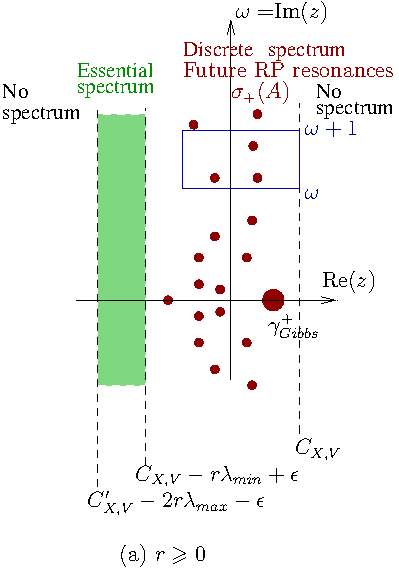
\includegraphics[scale=0.90]{figures/spectrum_Anosov_flow-1.pdf}}
\end{subfigure}
\hspace*{0.5mm}
\begin{subfigure}
{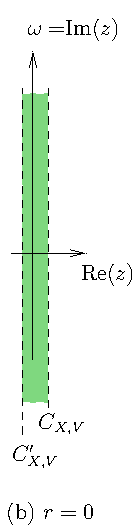
\includegraphics[scale=0.90]{figures/spectrum_r0-1.pdf}}
\end{subfigure}
\hspace*{0.5mm}
\begin{subfigure}
{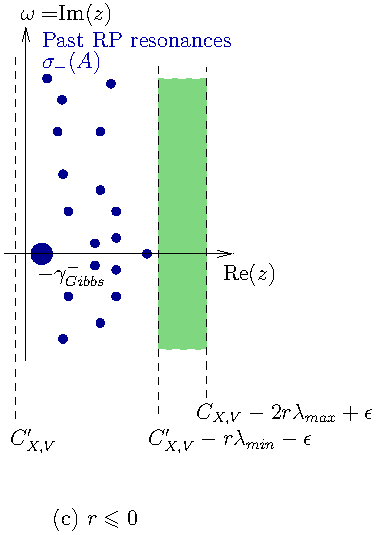
\includegraphics[scale=0.9]{figures/spectrum_Anosov_flow2-1.pdf}}
\end{subfigure}
\caption{Spectrum of $A=-X+V$ in $\clH _{W}(M)$, depending on $r\in\bbR$, with Anosov vector field $X$ and potential $V\in C(M;\bbC)$.\textbf{ (a):} For $r\protect\geq0$. $A$ has intrinsic discrete spectrum on $\Ree(z)>C_{X,V}-r\lambda_{\min}$ and a bounded resolvent on $\Ree(z)>C_{X,V}$ and $\Ree(z)<C'_{X,V}-2r\lambda_{\max}$. Theorem~\ref{thm:Weyl law} gives an upper bound for the number of resonances in the dashed rectangle, for $\omega\gg1$. As $r\rightarrow\infty$, the vertical band containing essential spectrum (in green) moves to the left and may reveal some new resonances. If $V$ is real valued then the rightmost (leading) eigenvalue is given by a topological pressure: $\gamma_{\Gibbs}^{+}=\Pr(V+\divv X_{/E_{s}})\in\bbR$.\textbf{ (b):} For $r=0$. Then $\clH _{W}(M)=L^{2}(M)$. The spectrum is contained in a vertical band~\eqref{eq:L2-spectrum}.\linebreak\textbf{(c):} For $r\protect\leq0$. Letting $r\rightarrow-\infty$ pushes the band containing the essential spectrum to the right, revealing Ruelle resonances for the past dynamics. If $V$ is real valued then the leftmost (leading) eigenvalue is $-\gamma_{\Gibbs}^{-}=-\Pr(-V-\divv X_{/E_{u}})$.}
\label{fig:discrete_spectrum}
\vspace*{-8pt}
\end{figure}

\begin{rema}
If $V$ is real-valued, the operator $A$ in~\eqref{eq:generator_A} commutes with the conjugation operator, hence the Ruelle spectrum is symmetric with respect to the real axis, as shown in Figure~\ref{fig:discrete_spectrum}. In this case, there is a leading real eigenvalue $\gamma_{\Gibbs}^{+}=\Pr(V+\divv X_{/_{E_{s}}})$ called Perron eigenvalue, where $\divv X_{/_{E_{s}}}<0$ is the divergence of $X$ measured on $E_{s}$ with respect to some (arbitrary) volume form. We observe this eigenvalue if we choose sufficiently large $r>0$ in the theorem above. Similarly, by considering the time-reversed system, we also find the leading real eigenvalue $-\gamma_{\Gibbs}^{-}$ with $\gamma_{\Gibbs}^{-}=\Pr(-V-\divv X_{/E_{u}})$, which we may call the Perron eigenvalue for the past and observe by letting $r<0$ be large. See Figure~\ref{fig:discrete_spectrum}.
\end{rema}


\begin{rema}[{``Relation between future and past spectrum''.}]
From the relation $\langle v|\clL^{t}u\rangle_{L^{2}(M)}=\langle(\clL^{t})^{\dagger}v|u\rangle_{L^{2}(M)}$ between
\[
\clL^{t}=e^{t\left(-X+V\right)}\quad\text{and}\quad\left(\clL^{t}\right)^{\dagger}=e^{t\left(X+\divv X+\overline{V}\right)},
\]
we can make the following observation. Assume that two potential functions $V,V'\in C^{\infty}(M;\bbC)$ satisfy the relation $V'+\overline{V}+\divv X=0$. Then the future spectrum $\sigma_{+}(A)$ of $A=-X+V$ is in one-to-one correspondence with the past spectrum $\sigma_{-}(A')$ of\linebreak $A'=-X+V'$ by the relation that $\lambda\in\sigma_{+}(A)$ if and only if $\lambda':=-\bar{\lambda}\in\sigma_{-}(A')$. Further the respective eigenprojectors, $\Pi_{\lambda}^{+}$ for $A$ and $\Pi_{\lambda'}^{-}$ for $A'$, are related by $\Pi_{\lambda'}^{-}=(\Pi_{\lambda}^{+})^{\dagger}$. In particular, if a potential function $V$ satisfies the condition $\Ree(V)=-\frac{1}{2}\divv X$, called ``half-density correction'', equivalently if $\clL^{t}:L^{2}(M)\rightarrow L^{2}(M)$ is unitary from~\eqref{eq:L*t*Lt}, then we have $A=A'=-X-\frac{1}{2}\divv X+i\Imm(V)$ and hence $\sigma_{+}(A)=-\overline{\sigma_{-}(A)}$.
\end{rema}


\break
\section{Anosov vector field}\label{subsec:Anosov_def}

\subsection{Definition of Anosov vector field}

Let $M$ be a $C^{\infty}$ compact connected manifold without boundary and let $n=\dim M-1$. Let $X$ be a $C^{\infty}$ non-vanishing vector field on $M$. The flow on $M$ generated by the vector field $X$ is denoted by
\begin{equation}\label{eq:flow_map}
\phi^{t}:=\exp\left(tX\right):\quad M\rightarrow M,\quad t\in\bbR.
\end{equation}
We make the assumption that $X$ is an Anosov vector field on $M$. This means that we have a continuous splitting of the tangent bundle
\begin{equation}\label{eq:decomp_TM}
TM=E_{u}\oplus E_{s}\oplus\underbrace{\bbR X}_{E_{0}},
\end{equation}
that is invariant by the flow $\phi^{t}$ and there exist $\lambda_{\min}>0$, $C>0$ and a smooth metric $g_{M}$ on $M$ such that
\begin{equation}\label{eq:hyperbolicity}
\begin{split}
\left\Vert d\phi_{/E_{u}\left(m\right)}^{-t}\right\Vert _{g_{M}} &\leq Ce^{-\lambda_{\min}t}\\
\text{and}\quad\left\Vert d\phi_{/E_{s}\left(m\right)}^{t}\right\Vert _{g_{M}} &\leq Ce^{-\lambda_{\min}t}\quad\text{for any }t\geq0,m\in M.
\end{split}
\end{equation}
See Figure~\ref{fig:Anosov-flow.}. The linear subspace $E_{u}(m),E_{s}(m)\subset T_{m}M$ are unique and called the unstable and stable space respectively. We set $E_{0}(m):=\bbR X(m)$ and call it the neutral direction or flow direction. In general, the maps $m\mapsto E_{u}(m)$, $m\mapsto E_{s}(m)$ and $m\mapsto E_{u}(m)\oplus E_{s}(m)$ are only H\"older continuous. We will write
\begin{equation}\label{eq:Holder_exp}
\beta_{u},\beta_{s},\beta_{0}\;\in\;]0,1]
\end{equation}
for the respective H\"older exponent. We have\footnote{We may expect that $\beta_{0}=\min(\beta_{u},\beta_{s})$ for generic Anosov flows. But this equality is not true in general. For instance, we have $\beta_{0}=1$ for contact Anosov flows, but $\min(\beta_{u},\beta_{s})$ will be smaller than $1$ in most of the cases because the (un)stable subspaces $E_{u}(m)$ and $E_{s}(m)$ will not be smooth.}
\begin{equation}\label{eq:def_beta_*}
\beta_{0}\geq\min\left(\beta_{u},\beta_{s}\right).
\end{equation}
See~\cite{hasselblatt1994regularity,hurder-90} for estimates on $\beta_{0},\beta_{u},\beta_{s}$.

\begin{figure}[h]
\centering
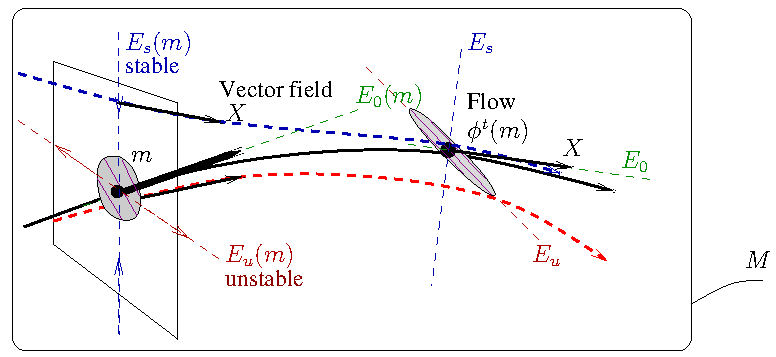
\includegraphics[scale=1.10]{figures/Anosov_flow_fig2-1.pdf} 
%\failedinput{figure/Anosov_flow_fig2.pdftex_t}
\caption{Anosov flow $\phi^{t}$ generated by a vector field $X$ on a compact manifold $M$.}
\label{fig:Anosov-flow.}
\end{figure}
Let $\scrA\in C^{0}(M;T^{*}M)$ be the continuous one form on $M$ called Anosov one form, which is defined for each $m\in M$ by the conditions
\begin{equation}\label{eq:one_form}
\scrA\left(m\right)\left(X\left(m\right)\right)=1\quad\text{and}\quad\Kerr\left(\scrA\left(m\right)\right)=E_{u}\left(m\right)\oplus E_{s}\left(m\right).
\end{equation}
By definition the Anosov one form $\scrA$ is preserved by the flow $\phi^{t}$ and the map $m\in M\mapsto\scrA(m)\in T^{*}M$ is H\"older continuous with exponent $\beta_{0}$.

\subsection{Transfer operator}\label{subsec:Transfer-operator}

Let $V\in C^{\infty}(M;\bbC)$ be an arbitrary smooth function, which is called a potential function. For $t\in\bbR$, let us denote the time integral of $V$ along the trajectory of $m\in M$ by
\begin{equation}\label{eq:time_averaged}
V_{\left[-t,0\right]}\left(m\right):=\int_{-t}^{0}V\left(\phi^{s}\left(m\right)\right)ds.
\end{equation}
For a given function $u\in C^{\infty}(M)$, $t\in\bbR$, $m\in M$, we consider the forward transported and amplitude modulated function along the trajectory:
\[
u_{t}\left(m\right):=\underbrace{e^{V_{\left[-t,0\right]}\left(m\right)}}_{\mathrm{amplitude}}\cdot\underbrace{\left(u\left(\phi^{-t}\left(m\right)\right)\right)}_{\mathrm{transport}}.
\]
\begin{center}
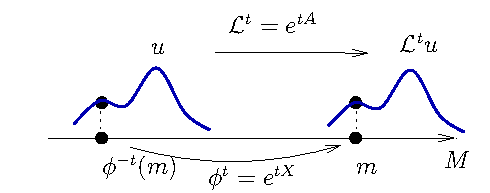
\includegraphics[scale=1]{figures/transf_op_3-1.pdf} 
\end{center}

Then we have $\frac{du_{t}}{dt}=(-X+V)u_{t}$ where the generating vector field $X$ is regarded as a first order differential operator\footnote{In local coordinates $x=(x_{1},\,\ldots x_{n})$ on $M$ we write $X=\sum_{j=1}^{\dim M}X_{j}(x)\frac{\partial}{\partial x^{j}}$.}. In other words, we have $u_{t}=\clL^{t}u$ for the one-parameter group of operators $\clL^{t}=\exp(tA)$ with generator $A=-X+V$. This gives the following definition.

\begin{cBoxA}{}
\begin{defi}[Ruelle transfer operator]\label{def:transfer_operator}
The one-parameter group of operators
\begin{equation}\label{eq:def_Transfer_operator}
\clL^{t}:
\begin{cases}
C^{\infty}\left(M\right) & \rightarrow C^{\infty}\left(M\right)\\
u & \mapsto e^{tA}u=e^{V_{\left[-t,0\right]}}\cdot\left(u\circ\phi^{-t}\right)
\end{cases}
\end{equation}
is called Ruelle transfer operators. It is generated by the first order differential operator on $C^{\infty}(M)$,
\begin{equation}\label{eq:generator_A}
A:=-X+V.
\end{equation}
\end{defi}
\end{cBoxA}

\begin{rema}
The results presented in this paper can be generalized for transfer operators acting on sections of a general (complex) vector bundle $E\rightarrow M$. We consider a linear operator acting on sections, $A:C^{\infty}(M;E)\rightarrow C^{\infty}(M;E)$, satisfying the Leibniz condition that for any function $f\in C^{\infty}(M;\bbC)$ and any section $s\in C^{\infty}(M;E)$, we have
\[
A\left(fs\right)=-X\left(f\right)s+fA\left(s\right).
\]
The group of transfer operators is defined by $\clL^{t}:=e^{tA}$ for $t\in\bbR$. With respect to a local frame $(e_{1},\,\ldots e_{m})$ of the vector bundle $E$ of rank $m$, a section is expressed as $s(x)=\sum_{j=1}^{m}u^{j}(x)e_{j}(x)$ with components $u^{j}(x)\in\bbC$. Then the operator $A$ is expressed as
\begin{equation}\label{eq:A_bundle}
\left(As\right)\left(x\right)=\sum_{j=1}^{m}\left(-\left(Xu^{j}\right)\left(x\right)+\sum_{k=1}^{m}V_{k}^{j}\left(x\right)u^{k}\left(x\right)\right)e_{j}\left(x\right)
\end{equation}
with a matrix of potential functions $V_{k}^{j}(x)\in\bbC$ defined by $(Ae_{k})(x)=\sum_{j}V_{k}^{j}(x)e_{j}(x)$. The expression~\eqref{eq:A_bundle} generalizes~\eqref{eq:generator_A}.
\end{rema}


\subsubsection*{Inverse and \texorpdfstring{$L^{2}$}{L2}-adjoint transfer operators}

Recall the time-averaged notation~\eqref{eq:time_averaged}. The inverse operator $\clL^{-t}$ that satisfies $\clL^{-t}\circ\clL^{t}=\Id _{/C^{\infty}(M)}$ is given by
\[
\clL^{-t}v\underset{\eqref{eq:def_Transfer_operator}}{=}e^{-V_{\left[-t,0\right]}\circ\phi^{t}}\left(v\circ\phi^{t}\right)=e^{-V_{\left[0,t\right]}}\left(v\circ\phi^{t}\right).
\]

Using an arbitrary smooth measure $dm$ on $M$ we define the $L^{2}$ scalar product: $\langle u|v\rangle_{L^{2}(M,dm)}:=\int_{M}\overline{u}vdm$ for $u,v\in C^{\infty}(M)$ and completion gives the space $L^{2}(M,dm)$. We define the formal adjoint operator $(\clL^{t})^{\dagger}:C^{\infty}(M)\rightarrow C^{\infty}(M)$ by
\[
\left\langle u\,\middle|\,\left(\clL^{t}\right)^{\dagger}v\right\rangle_{L^{2}}=\left\langle\clL^{t}u\,\middle|\,v\right\rangle_{L^{2}},\forall u,v\in C^{\infty}\left(M\right).
\]
We deduce that\footnote{With the change of variables $m'=\phi^{-t}(m)$ we get
\begin{align*}
\left\langle u\,\middle|\,\left(\clL^{t}\right)^{\dagger}v\right\rangle_{L^{2}} & =\left\langle\clL^{t}u\,\middle|\,v\right\rangle_{L^{2}}=\int e^{\overline{V_{\left[-t,0\right]}\left(m\right)}}\overline{u\left(\phi^{-t}\left(m\right)\right)}v\left(m\right)dm\\
& =\int e^{\overline{V_{\left[-t,0\right]}\left(\phi^{t}\left(m'\right)\right)}}\overline{u\left(m'\right)}v\left(\phi^{t}\left(m'\right)\right)\left|\det d\phi^{t}\left(m'\right)\right|dm'.
\end{align*}
}
\begin{align}
\left(\clL^{t}\right)^{\dagger}v & =e^{\overline{V_{\left[0,t\right]}}}\left|\det d\phi^{t}\right|\left(v\circ\phi^{t}\right)\label{eq:L2-adjoint_Lt}
\\
& =e^{\left(\overline{V}+\divv X\right)_{\left[0,t\right]}}\left(v\circ\phi^{t}\right)
\end{align}
where $\divv X$ is the divergence of the vector field $X$ with respect to $dm$. So
\begin{align}
\left(\clL^{t}\right)^{\dagger}&=e^{\left(2\Ree\left(V\right)+\divv X\right)_{\left[0,t\right]}}\clL^{-t}
\\
\intertext{and}
\left(\clL^{t}\right)^{\dagger}\circ\clL^{t}&=\clM_{\exp\left(2\varphi_{\left[0,t\right]}\right)}\label{eq:L*t*Lt}
\end{align}
is a multiplication operator by the function $\exp\left(2\varphi_{\left[0,t\right]}\right)\in C^{\infty}\left(M;\bbC\right)$ with
\begin{equation}\label{eq:def_At}
\varphi=\frac{1}{2}\divv X+\Ree\left(V\right).
\end{equation}
This expression explains the result~\eqref{eq:L2-spectrum} that expresses the spectrum of $A$ in $L^{2}(M)$ and will be used again in the paper (in the proof of Lemma~\ref{lem:For-the-weight} and Theorem~\ref{thm:decay_outside_trapped_set}).

\section{Semi-classical analysis with wave-packets}\label{sec:Semiclassical-analysis-with}

In this section, we develop general tools and lemmas for a flow generated by a \emph{non vanishing smooth vector field $X$ }on a compact manifold $M$. So we do not assume that $X$ is Anosov. In Subsection~\ref{subsec:Resolution-of-identity}, we introduce a wave-packet transform that gives a representation of distributions $u\in\clD'(M)$ as smooth functions on the cotangent space $T^{*}M$. The definition of our wave-packet transform is based on a metric $g$ on $T^{*}M$ that has a nice property called ``slowly varying''. We will introduce the metric $g$ in Subsection~\ref{subsec:A-metric}. In Subsection~\ref{subsec:Pseudo-differential-operator}, we give the definition of pseudo-differential operators (PDO) using the wave-packet transform and prove a useful theorem on compositions of PDO. In Subsection~\ref{subsec:Sobolev-space}, we define the Sobolev space $\clH _{W}(M)$ associated to a weight function $W$ on $T^{*}M$. In Section~\ref{subsec:A-matrix-elements}, we give a fundamental ``micro-local property'' of the transfer operator $\clL^{t}$ and prove a version of Egorov's theorem. The former micro-local property shows that the kernel of the operator induced on the phase space by $\clL^{t}$ decays very fast on the outside of the graph of the lifted flow $\tilde{\phi}^{t}:T^{*}M\rightarrow T^{*}M$. In Subsection~\ref{subsec:Strongly-continuous-semi-group}, we show that the transfer operators $\clL^{t}$ form a strongly continuous (semi-)group on $\clH _{W}(M)$ if the weight function $W$ satisfies some reasonable conditions with respect to the lifted flow $\tilde{\phi}^{t}:T^{*}M\rightarrow T^{*}M$.

The key results of this section are the resolution of identity in $C^{\infty}(M)$ given in Lemma~\ref{prop:resolution_identity_CM} and micro-locality of the transfer operator given in Lemma~\ref{thm:Microlocality-of-the_TO}.

\subsection{Wave packets transform and resolution of identity in \texorpdfstring{$T^{*}M$}{T*M}}\label{subsec:Resolution-of-identity}

\subsubsection{Flow box coordinates}

In this section we first introduce charts on the manifold $M$ and a partition of unity in order to decompose each function on $M$ into those supported on a single chart. Below we write $\bbR_{x}^{n}$ to indicate that we use the variable name $x$ for points on $\bbR^{n}$ and write $\bbB _{x}^{n}(c):=\{ x\in\bbR^{n},|x|<c\} $ for the open ball of radius $c>0$ in $\bbR_{x}^{n}$.

\begin{lemm}[{Flow box coordinates
\cite[p.~33]{taylor_tome1}}]\label{lem:charts}
For $c>0$ and $l>0$ small enough, there exist open subsets $U_{j}\subset M$ such that $M=\bigcup_{j=1}^{J}U_{j}$ and $C^{\infty}$ local charts diffeomorphism
\begin{equation}\label{eq:def_kappa_j}
\kappa_{j}:
\begin{cases}
U_{j}\subset M & \rightarrow V_{j}=\bbB _{x}^{n}\left(c\right)\times\bbB _{z}^{1}\left(l\right)\subset\bbR_{x}^{n}\times\bbR_{z}\\
\mkern40mu m & \to y\;\,=\left(x,z\right)
\end{cases}
\end{equation}
such that
\begin{equation}\label{eq:X}
\left(\kappa_{j}\right)_{*}\left(-X\right) =\frac{\partial}{\partial z}.
\end{equation}
and the $\kappa_{j}$ can be extended to a small neighborhood of $U_{j}$ (such coordinates are said to be admissible).
\end{lemm}

The next lemma introduces the operators $I$ and $I^{*}$ that decompose and reconstruct functions with respect to the charts (defined in Lemma~\ref{lem:charts}).


\begin{lemm}[Quadratic partition of unity]\label{lem:I-I*}
For the local charts $\kappa_{j}:U_{j}\to V_{j}$, $1\le j\le J$, given in Lemma~\ref{lem:charts}, there exist functions $\chi_{j}\in C_{0}^{\infty}(V_{j};\bbR^{+})$ for $1\le j\le J$, which give a quadratic partition of unity in the sense that
\begin{equation}\label{eq:partition_quadratic_unity-1}
\sum_{j:\,m\,\in\,U_{j}}\left(\left(\chi_{j}\circ\kappa_{j}\right)\left(m\right)\right)^{2}\left|\det d\kappa_{j}\left(m\right)\right|=1\quad\text{for all }m\in M
\end{equation}
where $|\det d\kappa_{j}(m)|=d\kappa_{j}^{*}(\Lebb)/dm$. For every $j\in\{ 1,\,\ldots J\} $, let
\begin{equation}\label{eq:def_I-2}
I_{j}:
\begin{cases}
C^{\infty}\left(M\right) & \rightarrow C_{0}^{\infty}\left(V_{j}\right)\\
u & \mapsto v_{j}\left(y\right):=\chi_{j}\left(y\right)\cdot\left(u\circ\kappa_{j}^{-1}\right)\left(y\right),
\end{cases}
\end{equation}
and
\begin{equation}\label{eq:def_I_1}
I:=\left(I_{j}\right)_{j}\,:C^{\infty}\left(M\right)\rightarrow\bigoplus_{j=1}^{J}C_{0}^{\infty}\left(V_{j}\right).
\end{equation}
Then the $L^{2}$-adjoint of $I:L^{2}(M,dm)\rightarrow\bigoplus_{j}L^{2}(V_{j},dy)$ is given by
\begin{equation}\label{eq:def_I*-2}
I^{\dagger}:
\begin{cases}
\bigoplus_{j}C_{0}^{\infty}\left(V_{j}\right) & \rightarrow C^{\infty}\left(M\right)\\
v=\left(v_{j}\right)_{j} & \mapsto u\left(m\right)=\sum_{j}\left(\chi_{j}\circ\kappa_{j}\right)\left(m\right)\cdot\left(v_{j}\circ\kappa_{j}\right)\left(m\right)\left|\det d\kappa_{j}\left(m\right)\right|
\end{cases}
\end{equation}
and we have
\begin{equation}\label{eq:I*_I}
I^{\dagger}\circ I=\Id _{/C^{\infty}\left(M\right)}.
\end{equation}
\end{lemm}

\begin{proof}
Let us consider functions $\chi_{j}^{(0)}\in C_{0}^{\infty}(V_{j};\bbR^{+})$ for $1\leq j\leq J$ such that
\[
S\left(m\right):=\sum_{j:\,m\,\in\,U_{j}}\left(\left(\chi_{j}^{\left(0\right)}\circ\kappa_{j}\right)\left(m\right)\right)^{2}\left|\det d\kappa_{j}\left(m\right)\right|>0
\]
for every $m\in M$. Then $\chi_{j}(x):=\chi_{j}^{(0)}(x)/\sqrt{S(\kappa_{j}(x))}$ satisfies~\eqref{eq:partition_quadratic_unity-1}. For $u\in C^{\infty}(M)$ and $v=(v_{j})\in\bigoplus_{j}C_{0}^{\infty}(V_{j})$, we have
\begin{align*}
\left\langle Iu|v\right\rangle _{\bigoplus_{j}L^{2}\left(V_{j}\right)} \underset{\eqref{eq:def_I-2}}{=}& \sum_{j}\left(\chi_{j}\cdot\left(u\circ\kappa_{j}^{-1}\right),v_{j}\right)_{L^{2}\left(V_{j}\right)}=\sum_{j}\int_{V_{j}}\chi_{j}\cdot\overline{\left(u\circ\kappa_{j}^{-1}\right)}\cdot v_{j}dy\\
 =& \int_{M}\sum_{j}\left(\chi_{j}\circ\kappa_{j}\right)\cdot\overline{u}\cdot\left(v_{j}\circ\kappa_{j}\right)\left|\det d\kappa_{j}\left(m\right)\right|dm\underset{\eqref{eq:def_I*-2}}{=}\left\langle u|I^{\dagger}v\right\rangle _{L^{2}\left(M\right)}
\end{align*}
and
\begin{align*}
\left(I^{\dagger}\circ I\right)u & \underset{\eqref{eq:def_I-2}\eqref{eq:def_I*-2}}{=}\sum_{j}\left(\chi_{j}\circ\kappa_{j}\right)\cdot\left(\left(\chi_{j}\circ\kappa_{j}\right)\cdot u\right)\left|\det d\kappa_{j}\right|\\
& =u\sum_{j}\left(\chi_{j}\circ\kappa_{j}\right)^{2}\left|\det d\kappa_{j}\right|\underset{\eqref{eq:partition_quadratic_unity-1}}{=}u.
\end{align*}
This completes the proof of Lemma~\ref{lem:I-I*}.
\end{proof}

In the following, we will consider the flow box coordinates $\kappa_{j}$ on the manifold $M$ and the associated quadratic partition of unity $\chi_{j}$ given by the two lemmas above.

\begin{rema}\label{rem:Projection}
We will find relations similar to~\eqref{eq:I*_I} a few times in the course of the argument below. Here we note that the relation~\eqref{eq:I*_I} can be interpreted as follows. The operator $I:L^{2}(M,dm)\rightarrow\bigoplus_{j}L^{2}(V_{j},dy)$ is an isometry onto this image because $\Vert Iu\Vert ^{2}=\langle Iu|Iu\rangle=\langle u|I^{\dagger}Iu\rangle\underset{\eqref{eq:I*_I}}{=}\left\Vert u\right\Vert ^{2}$. If we define
\[
P:=I\circ I^{\dagger}\quad:\bigoplus_{j}L^{2}\left(V_{j},dy\right)\rightarrow\bigoplus_{j}L^{2}\left(V_{j},dy\right),
\]
we have $P^{\dagger}=P$ and $P^{2}=P$ meaning that $P$ is the orthogonal projector on $\Imm(I)$. For the transfer operator $\clL^{t}:C^{\infty}(M)\rightarrow C^{\infty}(M)$ (or more generally for any linear operator), we consider the operator
\[
\tilde{\clL}^{t}:=I\circ\clL^{t}\circ I^{\dagger}.
\]
This is the simplest extension of $\clL^{t}$ in the sense that $\tilde{\clL}^{t}$ preserves the decomposition $\oplus_{j}C_{0}^{\infty}(V_{j})=\Imm(I)\oplus\Kerr(P)$, its restriction $\tilde{\clL^{t}}_{/\Imm(I)}$ is conjugated to $\clL^{t}$ and the restriction $\tilde{\clL^{t}}_{/\Kerr(P)}$ is the null operator. In other terms, $\tilde{\clL^{t}}=(I\circ\clL^{t}\circ I^{-1})\oplus0$ where $I^{-1}=I_{/\Imm(I)}^{\dagger}$. We may therefore regard the operator $\tilde{\clL}^{t}$ as a lifted representative (or a trivial extension) of $\clL^{t}$.
\end{rema}

\begin{defi}[Local coordinates on $T^{*}M$]\label{def:local_charts_on_T*M}
Let $\kappa_{j}:m\in U_{j}\mapsto y=(x,z)\in V_{j}\subset\bbR^{n}\times\bbR$ be the local flow-box coordinates in Lemma~\ref{lem:charts}. We write $\eta=(\xi,\omega)\in\bbR^{n}\times\bbR$ for the dual coordinates of $y=(x,z)\in\bbR^{n}\times\bbR$. Then the map $\kappa_{j}$ in~\eqref{eq:def_kappa_j} has a canonical extension to the cotangent bundle:
\begin{equation}\label{eq:def_k_tilde_j}
\tilde{\kappa_{j}}:
\begin{cases}
T^{*}U_{j} & \rightarrow T^{*}V_{j}=\bbB _{x}^{n}\left(c\right)\times\bbB _{z}^{1}\left(l\right)\times\bbR_{\xi}^{n}\times\bbR_{\omega}\\
\rho & \mapsto\varrho=\left(y,\eta\right)=\left(\left(x,z\right),\left(\xi,\omega\right)\right)
\end{cases}.
\end{equation}
We will regard these as local coordinates on $T^{*}M$. We will henceforth use the notation $\rho\in T^{*}U_{j}$ for a point on $T^{*}M$ and $\varrho=(y,\eta)\in T^{*}V_{j}$ for the corresponding point in a local chart as above. The canonical volume form on the cotangent bundle $T^{*}M$ will be denoted by
\begin{equation}\label{eq:def_d_rho}
d\rho:=\left(\tilde{\kappa_{j}}\right)^{*}\left(d\varrho\right)\quad\text{with}\quad d\varrho:=\left(\Pi_{k=1}^{n}dx_{k}\wedge d\xi_{k}\right)\wedge dz\wedge d\omega.
\end{equation}
\end{defi}


\subsubsection{\label{subsec:A-metric}
A global metric \texorpdfstring{$g$}{g} on \texorpdfstring{$T^{*}M$}{T*M}}

For a given chart index $j$, using the local charts~\eqref{eq:def_k_tilde_j}, we have already defined the metric $g$ on $T^{*}\bbR^{n+1}=\bbR_{y}^{n+1}\times\bbR_{\eta}^{n+1}$ in~\eqref{eq:metric_g_in_coordinates}. We write $g_{j}:=\kappa_{j}^{*}(g)$ for the metric induced on $T^{*}U_{j}$, i.e. at a given point $\rho\in T^{*}U_{j}$, it is given by
\[
g_{j,\rho}\left(u_{1},u_{2}\right):=g_{\varrho}\left(d\tilde{\kappa_{j}}\left(u_{1}\right),d\tilde{\kappa_{j}}\left(u_{2}\right)\right)\quad\text{for }u_{1},u_{2}\in T_{\rho}\left(T^{*}M\right).
\]
We will prove below in~\eqref{eq:equiv_g_tilde} that the metric $g_{j}$ and $g_{j'}$ are uniformly equivalent on $U_{j}\cap U_{j'}$. Then we define the following global metric $g$ on $T^{*}M$ (abusively we use the same letter $g$)
\begin{equation}\label{eq:global_metric}
g:=\sum_{j=1}^{J}\left(\chi_{j}^{2}\circ\kappa_{j}\circ\pi\right)\cdot g_{j}
\end{equation}
where $\pi:T^{*}M\to M$ denotes the bundle projection. The global metric $g$ in~\eqref{eq:global_metric} will provide the size of wave packets to our analysis of the transfer operator over the manifold $M$. We will write $\dist_{g}(\rho,\rho')$ for the geodesic distance between $\rho,\rho'\in T^{*}M$ defined from this metric $g$.

We will give now few essential properties of the metric $g$.

\begin{cBoxB}{}
\begin{lemm}\label{thm:The-metric-}
The Riemann metric $g$ on $T^{*}M$ is \emph{geodesically complete}.
\end{lemm}
\end{cBoxB}

\begin{proof}
Let $g_{M}$ be a Riemann metric on $M$. Consider the function $\Gamma:T^{*}M\rightarrow\bbR^{+}$ given by
\begin{equation}\label{eq:def_Gamma}
\Gamma\left(\rho\right)=\left\Vert \rho\right\Vert _{g_{M}}^{1-\alpha^{\perp}}\asymp\left|\eta\right|^{1-\alpha^{\perp}},
\end{equation}
using local coordinates $\rho=(y,\eta)$ with $|\eta|>1$. From~\eqref{eq:conditions}, we have $1-\alpha^{\perp}>0$ so that $\Gamma$ increases with $\Vert \rho\Vert _{g_{M}}$. There exists $C,C'>0$ such that for any $v\in TT^{*}M$, with local components $(v_{y},v_{\eta})$, we have, using also $1-\alpha^{\perp}\leq\alpha^{\perp}$ from~\eqref{eq:conditions},
\begin{equation}\label{eq:bound-3}
\begin{split}
\left|d\Gamma\left(v\right)\right|&\underset{\eqref{eq:def_Gamma}}{\leq}C'\left(\left|\eta\right|^{1-\alpha^{\perp}}\left|v_{y}\right|+\left|\eta\right|^{-\alpha^{\perp}}\left|v_{\eta}\right|\right)\\
&\;\underset{\eqref{eq:conditions}}{\leq}C'\left(\left|\eta\right|^{\alpha^{\perp}}\left|v_{y}\right|+\left|\eta\right|^{-\alpha^{\perp}}\left|v_{\eta}\right|\right)\underset{\eqref{eq:metric_g_in_coordinates}}{\leq}C\left\Vert v\right\Vert _{g}.
\end{split}
\end{equation}
For any $A>0$, the set $R_{A}:=\{ \rho\in T^{*}M,\Gamma(\rho)\in[0,A]\} $ is compact. Take any point $\rho\in T^{*}M$ and consider $\gamma:t\mapsto\gamma(t)\in T^{*}M$ a unit speed geodesic starting at $\rho$, i.e. $\Vert \dot{\gamma}\Vert _{g}=1$. Then $|d\Gamma(\dot{\gamma})|\underset{\eqref{eq:bound-3}}{\leq}C\Vert \dot{\gamma}\Vert _{g}\leq C$ so for any $t\geq0$,
\[
\big|\Gamma\left(\gamma\left(t\right)\right)-\Gamma\left(\gamma\left(0\right)\right)\big|=\left|\int_{0}^{t}d\Gamma\left(\dot{\gamma}\right)dt'\right|<Ct
\]
i.e. $\gamma(t)\in R_{A}$ with $A=\Gamma(\gamma(0))+Ct$. This shows that the time to reach the boundary of $R_{A}$ tends to $\infty$ as $A\rightarrow\infty$. This implies that the geodesic is defined for every $t\in\bbR$, i.e. the metric $g$ is geodesically complete.
\end{proof}

\subsubsection{\label{subsec:Lipschitz-property-of}
Lipschitz property of \texorpdfstring{$g$}{g} with respect to the flow map and change of charts.}

The push-forward action of the flow $\phi^{t}=e^{tX}:M\rightarrow M$ on the cotangent space $T^{*}M$ is denoted by
\begin{equation}\label{eq:lifted_flow}
\tilde{\phi}^{t}:
\begin{cases}
T^{*}M & \rightarrow T^{*}M,\\
\mkern20mu\rho & \mapsto\rho\left(t\right):=\left(\left(d_{m}\phi^{t}\right)^{*}\right)^{-1}\rho.
\end{cases}
\end{equation}
with $m=\pi(\rho)$. In this section we will prove the following lemma.

\begin{cBoxB}{}
\begin{lemm}[Lipschitz property of $g$]\label{lem:Lipschitz_property}
From the conditions~\eqref{eq:conditions} we have that for any $t\in\bbR$, there exists a constant $C_{t}>0$ such that for any $\rho,\rho'\in T^{*}M$,
\begin{equation}\label{eq:invariance_g}
\dist_{g}\left(\tilde{\phi}^{t}(\rho),\tilde{\phi}^{t}(\rho')\right)\le C_{t}\dist_{g}\left(\rho,\rho'\right).
\end{equation}
\end{lemm}
\end{cBoxB}

\begin{rema}
Property~\eqref{eq:invariance_g} will be crucial to get Lemma~\ref{lem:Description-of-evolving} below. This property means that the pulled back metric $(\tilde{\phi}^{t})^{\circ}g$ is equivalent to the metric $g$ uniformly with respect to $\rho\in T^{*}M$. Equivalently one can write
\[
\forall t\in\bbR,\exists C_{t}>0,\forall\rho\in T^{*}M,\quad\left\Vert d\tilde{\phi}^{t}\left(\rho\right)\right\Vert _{g}\leq C_{t},
\]
or infinitesimally with the vector field $\tilde{X}$ that is $X$ lifted on $T^{*}M$ (i.e. the generator of $\tilde{\phi}^{t}$) acting as the Lie derivative $\clL_{\tilde{X}}$ on $g$,
\[
\exists C>0,\forall\rho\in T^{*}M,\quad\left\Vert \left(\clL_{\tilde{X}}g\right)\left(\rho\right)\right\Vert _{g}\leq C,
\]
and this is true more generally for any local change of flow box coordinate as given below in~\eqref{eq:coordinate_change} or for a local diffeomorphism on $M$ that preserves the vector field~$X$.
\end{rema}

\begin{proof}
In order to prove Lemma~\ref{lem:Lipschitz_property}, remark first that for any chart indices $j,j'\in\{1,\,\ldots J\} $ with $U_{j}\cap U_{j'}\neq\emptyset$, the expression of the metric in~\eqref{eq:metric_g_in_coordinates} gives different metrics $g_{j}=\kappa_{j}^{*}(g)$, $g_{j'}=\kappa_{j'}^{*}(g)$ on different charts. We will show that conditions~\eqref{eq:conditions} guaranty that these metrics are uniformly equivalent in the sense that $\exists C>0,\forall\rho\in T^{*}(U_{j}\cap U_{j'})$, $\forall u\in T_{\rho}(T^{*}M)$,
\begin{equation}\label{eq:equiv_g_tilde}
\frac{1}{C}\left\Vert u\right\Vert _{g_{j}}\leq\left\Vert u\right\Vert _{g_{j'}'}\leq C\left\Vert u\right\Vert _{g_{j}}.
\end{equation}

\begin{rema}\label{rem:asympt}
We will express the relation~\eqref{eq:equiv_g_tilde} as $\Vert u\Vert _{g_{j}}\asymp\Vert u\Vert _{g_{j'}}$ by using the notation $\asymp$.
\end{rema}

Let us consider a local change of coordinates $(x,z)\mapsto(x',z')$ between the flow box coordinates in Lemma~\ref{lem:charts}. It is written in the form
\begin{equation}\label{eq:coordinate_change}
x'=f\left(x\right),\quad z'=z+h\left(x\right)
\end{equation}
using a smooth diffeomorphism $f:\bbR^{n}\rightarrow\bbR^{n}$ and a smooth function $h:\bbR^{n}\rightarrow\bbR$. By compactness of $M$, we may and do assume that $f$ and $h$ are bounded in the $C^{2}$ sense. From~\eqref{eq:coordinate_change}, we have
\begin{equation}\label{eq:relation_coordinates}
dx'=\left(d_{x}f\right)dx,\quad dz'=dz+\left(d_{x}h\right)dx.
\end{equation}
Let us write $(x,z,\xi,\omega)\to(x',z',\xi',\omega')$ for the induced coordinate change on the cotangent bundle. Then the relation
\[
\xi dx+\omega dz=\xi'dx'+\omega'dz'=\left(\left(d_{x}f\right)^{T}\xi'+\left(d_{x}h\right)\omega'\right)dx+\omega'dz
\]
gives
\begin{equation}\label{eq:dd}
\xi=\left(d_{x}f\right)^{T}\xi'+\left(d_{x}h\right)\omega'\quad\text{and}\quad\omega=\omega'.
\end{equation}
Hence we find
\begin{equation}\label{eq:relation_coordinates2}
\begin{split}
d\xi & =\left(\left(d_{x'}\left(d_{x}f\right)^{T}\right)\xi'+\left(d_{x'}\left(d_{x}h\right)\right)\omega'\right)dx'+\left(d_{x}f\right)^{T}d\xi'+\left(d_{x}h\right)d\omega',
\\
d\omega & =d\omega'.
\end{split}
\end{equation}
From $C^{2}$ boundedness of $f$ and $h$, we have $\langle \eta\rangle \asymp\langle \eta'\rangle $ for $\eta=(\xi,\omega)$ and $\eta'=(\xi',\omega')$ and hence
\begin{equation}\label{eq:equivalence_of_delta}
\delta^{\perp}\left(\eta\right)\asymp\delta^{\perp}\left(\eta'\right),\quad\delta^{\parallel}\left(\eta\right)\asymp\delta^{\parallel}\left(\eta'\right).
\end{equation}
To compare $g$ and $g'$, we rewrite the relations~\eqref{eq:relation_coordinates} and~\eqref{eq:relation_coordinates2} as
\begin{align*}
\frac{dx'}{\delta^{\perp}\left(\eta\right)} & =d_{x}f\left(\frac{dx}{\delta^{\perp}\left(\eta\right)}\right)\asymp\frac{dx}{\delta^{\perp}\left(\eta\right)},\\
\frac{dz'}{\delta^{\parallel}\left(\eta\right)} & =\frac{dz}{\delta^{\parallel}\left(\eta\right)}+\frac{\delta^{\perp}\left(\eta\right)}{\delta^{\parallel}\left(\eta\right)}\cdot d_{x}h\left(\frac{dx}{\delta^{\perp}\left(\eta\right)}\right),\\
\delta^{\perp}\left(\eta\right)d\xi & =\left((\delta^{\perp}\left(\eta\right))^{2}\left(d_{x'}\left(d_{x}f\right)^{T}(\xi')+d_{x'}\left(d_{x}h(\omega')\right)\right)\right)\cdot\frac{dx'}{\delta^{\perp}\left(\eta\right)}\\
& \qquad+\delta^{\perp}\left(\eta\right)\left(d_{x}f\right)^{T}\left(d\xi'\right)+\frac{\delta^{\perp}\left(\eta\right)}{\delta^{\parallel}\left(\eta\right)}\left(d_{x}h\right)\left(\delta^{\parallel}\left(\eta\right)d\omega'\right).
\end{align*}
Therefore, in order that $g_{\varrho}\preceq g'_{\varrho'}$, a necessary and sufficient condition is that
\begin{equation}\label{eq:requirement}
(\delta^{\perp}\left(\eta\right))^{2}\left|\xi'\right|\leq C\quad\text{and}\quad(\delta^{\perp}\left(\eta\right))^{2}\left|\omega'\right|\leq C\quad\text{and}\quad\frac{\delta^{\perp}\left(\eta\right)}{\delta^{\parallel}\left(\eta\right)}\leq C.
\end{equation}
Since the former two inequalities are written
\[
\delta^{\perp}\left(\eta\right)\leq C\min\left\{ \left|\xi'\right|^{-1/2},\left|\omega'\right|^{-1/2}\right\}
\]
we see that the last condition~\eqref{eq:requirement} is equivalent to the condition
\[
1/2\leq\alpha^{\perp}\quad\text{and}\quad0\leq\alpha^{\parallel}\leq\alpha^{\perp}.
\]
that was assumed in~\eqref{eq:conditions}. We have obtained~\eqref{eq:equiv_g_tilde}. Since the flow $\phi^{t}$ viewed in the local charts $\kappa_{j}$ is also written in the form~\eqref{eq:coordinate_change} we get Lemma~\ref{lem:Lipschitz_property}.
\end{proof}

\subsubsection{Moderate and temperate properties of the metric \texorpdfstring{$g$}{g}}

Now we will discuss so called moderate and temperate properties of the metric $g$.

\begin{rema}
The metric $g$ that we have introduced is similar to the so-called symplectic metric $g^{\natural}$ introduced in semi-classical analysis by H\"ormander, see~\cite[Defi.~2.2.19, p.~78]{lerner2011metrics}, \cite[Chap.~XVIII]{hormander_3}, \cite{nicola_rodino_livre_11}. Temperate, slowly varying and moderate properties of the metric are discussed in these books for the purpose of semi-classical analysis.
\end{rema}

\begin{cBoxA}{}
\begin{defi}[Distortion function $\Delta:T^{*}M\rightarrow\bbR^{+}$]
For $\rho\in T^{*}M$, set
\begin{equation}\label{eq:def_distortion_function_D}
\Delta\left(\rho\right):=\left\langle \left\Vert \rho\right\Vert _{g_{M}}\right\rangle ^{-\left(1-\alpha^{\perp}\right)}.
\end{equation}
where $g_{M}$ is a Riemannian metric on $M$.
\end{defi}
\end{cBoxA}

Observe that $\Delta(\rho)\rightarrow0$ when $\Vert \rho\Vert _{g_{M}}\rightarrow\infty$. For practical purpose we can also define a distortion function in local chart using the same expression:


\begin{defi}[Distortion function $\Delta:\bbR^{2(n+1)}\rightarrow\bbR^{+}$
in local chart] For $\varrho=(y,\eta)\in\bbR^{2(n+1)}$, we set
\begin{equation}\label{eq:def_distortion_function_D-1}
\Delta\left(\varrho\right):=\delta^{\perp}\left(\eta\right)^{\left(1/\alpha^{\perp}\right)-1}\eq{\ref{eq:def_delta}}\left\langle \left|\eta\right|\right\rangle ^{-\left(1-\alpha^{\perp}\right)}.
\end{equation}

From~\eqref{eq:equivalence_of_delta}, we have that the equivalence $\Delta(\rho)\asymp\Delta(\varrho)$ for $\varrho=(y,\eta)=\tilde{\kappa}_{j}\left(\rho\right)$ with any chart index $j$.
\end{defi}

The next lemma shows that the distortion function $\Delta(\varrho)$ is related to the variation of the metric $g$ on $T^{*}\bbR^{n+1}=\bbR^{(n+1)}$ with respect to itself. Recall the notation $\langle s\rangle :=(1+s^{2})^{1/2}$ for $s\in\bbR$ introduced in~\eqref{eq:def_Japonese_bracket}.

\begin{cBoxB}{}
\begin{lemm}[The metric $g$ is $\Delta^{\gamma}$-moderate and temperate]\label{lem:temperate_metric}
For any $0\leq\gamma<1$, there exist $N>0$ and $C>0$ such that
\begin{equation}\label{eq:g_moderate and temperate}
\max\left\{ \frac{\|v\|_{g_{\varrho'}}}{\|v\|_{g_{\varrho}}},\frac{\|v\|_{g_{\varrho}}}{\|v\|_{g_{\varrho'}}}\right\} \le1+C\Delta(\varrho)^{1-\gamma}\left\langle \left(\Delta\left(\varrho\right)\right)^{\gamma}\left\Vert \varrho'-\varrho\right\Vert _{g_{\varrho}}\right\rangle ^{N}
\end{equation}
for any $\varrho,\varrho'\in\bbR^{2(n+1)}$ and $v\in\bbR^{2(n+1)}$. Consequently we have
\begin{align}\label{eq:equivalence_distance}
\frac{1}{C}\left\langle \left\Vert \varrho'-\varrho\right\Vert _{g_{\varrho}}\right\rangle ^{1/N}\leq & \left\langle \left\Vert \varrho'-\varrho\right\Vert _{g_{\varrho'}}\right\rangle \le C\left\langle \left\Vert \varrho'-\varrho\right\Vert _{g_{\varrho}}\right\rangle ^{N}.
\end{align}
\end{lemm}
\end{cBoxB}

\begin{rema}
The inequality~\eqref{eq:g_moderate and temperate} expresses two properties about the variation of $g$:
\begin{enumerate}
\item the moderate property (also called slowly varying property): if two points $\varrho,\varrho'$ are in a distance $\Vert \varrho'-\varrho\Vert _{g_{\varrho}}\leq\Delta^{\gamma}(\varrho)^{-1}$ then the ratio between $g_{\varrho},g_{\varrho'}$ is bounded and close to one at high frequencies. In other words the metric $g$ varies slowly at the scale of the metric itself.
\item the temperate property (at infinity) : the metric $g_{\varrho'}$ grows no faster than a power of $\Vert \varrho'-\varrho\Vert _{g_{\varrho}}$ (modified by the factor $\Delta^{\gamma}(\varrho)$) when $\varrho'\to\infty$.
\end{enumerate}
\end{rema}

\begin{proof}[Proof of Lemma~\ref{lem:temperate_metric}]
Let $v=((v_{x},v_{z}),(v_{\xi},v_{\omega}))\in\bbR^{2(n+1)}$ and $\varrho=(y,\eta),$ $\varrho'=(y',\eta')\in\bbR^{2(n+1)}$. Recall that $0\leq\alpha^{\parallel}\leq\alpha^{\perp}$ in~\eqref{eq:conditions}. We have
\begin{align*}
\|v\|_{g_{\varrho}}^{2} &\!\!\underset{\eqref{eq:metric_g_in_coordinates}}{=} \left(\frac{\left|v_{x}\right|}{\left\langle \left|\eta\right|\right\rangle ^{-\alpha^{\perp}}}\right)^{2}+\left(\left\langle \left|\eta\right|\right\rangle ^{-\alpha^{\perp}}\left|v_{\xi}\right|\right)^{2}+\left(\frac{\left|v_{z}\right|}{\left\langle \left|\eta\right|\right\rangle ^{-\alpha^{\parallel}}}\right)^{2}+\left(\left\langle \left|\eta\right|\right\rangle ^{-\alpha^{\parallel}}\left|v_{\omega}\right|\right)^{2}\\
&= \left(\frac{\left\langle \left|\eta\right|\right\rangle }{\left\langle \left|\eta'\right|\right\rangle }\right)^{2\alpha^{\perp}}\left(\frac{\left|v_{x}\right|}{\left\langle \left|\eta'\right|\right\rangle ^{-\alpha^{\perp}}}\right)^{2}+\left(\frac{\left\langle \left|\eta'\right|\right\rangle }{\left\langle \left|\eta\right|\right\rangle }\right)^{2\alpha^{\perp}}\left(\left\langle \left|\eta'\right|\right\rangle ^{-\alpha^{\perp}}\left|v_{\xi}\right|\right)^{2}\\
& \quad +\left(\frac{\left\langle \left|\eta\right|\right\rangle }{\left\langle \left|\eta'\right|\right\rangle }\right)^{2\alpha^{\parallel}}\left(\frac{\left|v_{z}\right|}{\left\langle \left|\eta'\right|\right\rangle ^{-\alpha^{\parallel}}}\right)^{2}+\left(\frac{\left\langle \left|\eta'\right|\right\rangle }{\left\langle \left|\eta\right|\right\rangle }\right)^{2\alpha^{\parallel}}\left(\left\langle \left|\eta'\right|\right\rangle ^{-\alpha^{\parallel}}\left|v_{\omega}\right|\right)^{2}\\
&\!\!\underset{\eqref{eq:conditions}}{\leq}  \max\left\{ \left(\frac{\langle|\eta'|\rangle}{\langle|\eta|\rangle}\right)^{2\alpha^{\perp}},\left(\frac{\langle|\eta|\rangle}{\langle|\eta'|\rangle}\right)^{2\alpha^{\perp}}\right\} \|v\|_{g_{\varrho'}}^{2}.
\end{align*}
We deduce that
\begin{equation}\label{eq:comparison}
\max\left\{ \frac{\|v\|_{g_{\varrho'}}}{\|v\|_{g_{\varrho}}},\frac{\|v\|_{g_{\varrho}}}{\|v\|_{g_{\varrho'}}}\right\} \underset{\eqref{eq:metric_g_in_coordinates}}{\leq}\max\left\{ \left(\frac{\langle|\eta'|\rangle}{\langle|\eta|\rangle}\right)^{\alpha^{\perp}},\left(\frac{\langle|\eta|\rangle}{\langle|\eta'|\rangle}\right)^{\alpha^{\perp}}\right\}.
\end{equation}
Below we estimate the ratios $\langle|\eta'|\rangle/\langle|\eta|\rangle$ and $\langle|\eta|\rangle/\langle|\eta'|\rangle$ to get the required estimate~\eqref{eq:g_moderate and temperate}. For the former, we have
\begin{align}
\frac{\langle|\eta'|\rangle}{\langle|\eta|\rangle}\underset{\eqref{eq:D1p}}{\leq}1+\frac{\left|\eta'-\eta\right|}{\langle|\eta|\rangle} & \underset{\eqref{eq:metric_g_in_coordinates}}{\leq}1+\frac{\langle\left|\eta\right|\rangle^{\alpha^{\perp}}\|\varrho'-\varrho\|_{g_{\varrho}}}{\left\langle \left|\eta\right|\right\rangle }\underset{\eqref{eq:def_distortion_function_D-1}}{=} 1+\Delta\left(\varrho\right)\|\varrho'-\varrho\|_{g_{\varrho}}\label{eq:res1-1}
\\
& \ineq{\ref{eq:prod}}1+\Delta(\varrho)^{1-\gamma}\cdot\langle\Delta(\varrho)^{\gamma}\|\varrho'-\varrho\|_{g_{\varrho}}\rangle.
\end{align}
For the latter, if $|\eta'|\ge\frac{1}{2}|\eta'-\eta|$ then $\langle|\eta|\rangle\leq\langle|\eta'|\rangle+|\eta'-\eta|\le3\langle|\eta'|\rangle$ and we can proceed similarly to the previous case:
\begin{align*}
\frac{\langle|\eta|\rangle}{\langle|\eta'|\rangle} &\leq1+\frac{\left|\eta'-\eta\right|}{\langle|\eta'|\rangle}\leq1+3\frac{\left|\eta'-\eta\right|}{\langle|\eta|\rangle}=1+3\Delta\left(\varrho\right)\|\varrho'-\varrho\|_{g_{\varrho}}\\
&\le1+3\Delta(\varrho)^{1-\gamma}\cdot\langle\Delta(\varrho)^{\gamma}\|\varrho'-\varrho\|_{g_{\varrho}}\rangle.
\end{align*}
Otherwise if $|\eta'|<\frac{1}{2}|\eta'-\eta|$ then $|\eta'-\eta|\leq|\eta'|+|\eta|\leq\frac{1}{2}|\eta'-\eta|+|\eta|$ and
\[
\frac{1}{2}|\eta'-\eta|\leq\left|\eta\right|=|\eta-\eta'+\eta'|\leq|\eta'-\eta|+|\eta'|\leq\frac{3}{2}|\eta'-\eta|,
\]
i.e. $|\eta|$ is comparable with $|\eta'-\eta|$. Hence, for any $N>0$, there exists a constant $C_{N}>0$ such that
\[
\begin{aligned}\frac{\langle|\eta|\rangle}{\langle|\eta'|\rangle} & \leq1+|\eta'-\eta|\leq1+C_{N}|\eta|^{-\mu_{N}}\cdot\left\langle \langle|\eta|\rangle^{-(1-\alpha^{\perp})\gamma}\langle|\eta|\rangle^{-\alpha^{\perp}}|\eta'-\eta|\right\rangle ^{N}\\
& \leq1+C_{N}|\eta|^{-\mu_{N}}\cdot\left\langle \Delta\left(\varrho\right)^{\gamma}\|\varrho'-\varrho\|_{g_{\varrho}}\right\rangle ^{N}
\end{aligned}
\]
where $\mu_{N}=N(1-\alpha^{\perp})(1-\gamma)-1.$ Letting $N$ be sufficiently large so that $\langle |\eta|\rangle ^{-\mu_{N}}\linebreak\leq\Delta(\varrho)^{1-\gamma}$ we obtain
\[
\frac{\langle|\eta|\rangle}{\langle|\eta'|\rangle}\le1+C_{N}\Delta(\varrho)^{1-\gamma}\langle\Delta\left(\varrho\right)^{\gamma}\|\varrho'-\varrho\|_{g_{\varrho}}\rangle^{N}.
\]
Summarizing the estimates above, we obtain~\eqref{eq:g_moderate and temperate}. In order to get~\eqref{eq:equivalence_distance}, we set $v=\varrho'-\varrho$ and $\gamma=0$ in~\eqref{eq:g_moderate and temperate}.
\end{proof}

In the previous lemma we have used $\Vert \varrho'-\varrho\Vert _{g_{\varrho}}$ that makes sense in a local chart. This quantity will appear later in the proof of Theorem~\ref{thm:Microlocality-of-the_TO} from some integration by parts. However to express the results, we would like to use the more geometrical quantity that is the geodesic distance $\dist_{g}(\rho',\rho)$ for the global metric $g$ in~\eqref{eq:global_metric}. The next lemma shows that both quantities are equivalent.

\begin{cBoxB}{}
\begin{lemm}\label{lem:There-exist-}
There exist $N>0$ and $C>0$ such that for every $\varrho=\tilde{\kappa_{j}}(\rho),\varrho'=\tilde{\kappa}_{j}(\rho')$,
\begin{equation}\label{eq:log_log}
\frac{1}{C}\left\langle \left\Vert \varrho'-\varrho\right\Vert _{g_{\varrho}}\right\rangle ^{1/N}\leq\left\langle \dist_{g}\left(\rho',\rho\right)\right\rangle \leq C\left\langle \left\Vert \varrho'-\varrho\right\Vert _{g_{\varrho}}\right\rangle ^{N},
\end{equation}
\end{lemm}
\end{cBoxB}

\begin{proof}
To show the second inequality in~\eqref{eq:log_log}, we consider the straight path $t\in[0,1]\mapsto\varrho(t)=(1-t)\varrho+t\varrho'$ and get that $\langle \dist_{g}(\rho',\rho)\rangle \leq C\langle \Vert \varrho'-\varrho\Vert _{g_{\varrho}}\rangle^{N}$ for some $C>0,N>0$. To show the first inequality in~\eqref{eq:log_log}, let us assume that $\rho:t\in[0,1]\mapsto\rho(t)$ is a geodesic from $\rho=\rho(0)$ to $\rho'=\rho(1)$. In a local chart $\varrho(t)=\tilde{\kappa_{j}}(\rho(t))=(y(t),\eta(t))\in\bbR^{n+1}\times\bbR^{n+1}$. We will use that for some $C>0$,
\begin{equation}\label{eq:bound-2}
\dist_{g}\left(\rho',\rho\right)
=\int_{0}^{1}\left\Vert \dot{\rho}\left(t\right)\right\Vert _{g_{\rho\left(t\right)}}dt
\geq C\left(\int_{0}^{1}\left\Vert \dot{y}\left(t\right)\right\Vert _{g_{\varrho\left(t\right)}}dt+\int_{0}^{1}\left\Vert \dot{\eta}\left(t\right)\right\Vert _{g_{\varrho\left(t\right)}}dt\right).
\end{equation}
We may assume without loss of generality that $|\eta'|=|\eta(1)|\geq|\eta(0)|=|\eta|$. Let us consider a few complementary cases.
\begin{enumerate}
\item If $\exists t'\in[0,1]$ such that $|\eta(t')|<\frac{1}{2}|\eta|$, then using the second integral in~\eqref{eq:bound-2}, we get that for some $C,N,C',N'>0$ we have
\[
\left\langle \dist_{g}\left(\rho',\rho\right)\right\rangle \ineqs{\ref{eq:equivalence_distance}}C\left\langle \frac{1}{2}\left\Vert \eta\right\Vert _{g_{\varrho}}\right\rangle ^{1/N}+C\left\langle \frac{1}{2}\left\Vert \eta'\right\Vert _{g_{\varrho}}\right\rangle ^{1/N}\geq C'\left\langle \left\Vert \varrho'-\varrho\right\Vert _{g_{\varrho}}\right\rangle ^{1/N'}.
\]
\item Otherwise $\forall t\in[0,1],$ $|\eta(t)|\geq\frac{1}{2}|\eta|$ and we consider two subcases:
\begin{enumerate}
\item If $\Vert y'-y\Vert _{g_{\varrho}}\geq\Vert \eta'-\eta\Vert _{g_{\varrho}}$ then $\Vert y'-y\Vert _{g_{\varrho}}\geq\frac{1}{2}\Vert \varrho'-\varrho\Vert _{g_{\varrho}}$. Using the first integral in~\eqref{eq:bound-2}, then for some $C,N>0$ we have
\begin{align*}
\left\langle \dist_{g}\left(\rho',\rho\right)\right\rangle & \geq\left\langle \left\Vert y'-y\right\Vert _{g_{\left(y,\frac{1}{2}\eta\right)}}\right\rangle \ineqs{\ref{eq:equivalence_distance}}\frac{1}{C}\left\langle \left\Vert y'-y\right\Vert _{g_{\varrho}}\right\rangle ^{1/N}\\
& \geq\frac{1}{C}\left\langle \left\Vert \varrho'-\varrho\right\Vert _{g_{\varrho}}\right\rangle ^{1/N}.
\end{align*}
\item Otherwise $\Vert \eta'-\eta\Vert _{g_{\varrho}}\geq\Vert y'-y\Vert _{g_{\varrho}}$ then $\Vert \eta'-\eta\Vert _{g_{\varrho}}\geq\frac{1}{2}\Vert \varrho'-\varrho\Vert _{g_{\varrho}}$ and for some $C,N>0$ we have
\begin{align*}
\left\langle \dist_{g}\left(\rho',\rho\right)\right\rangle & \geq\frac{1}{C}\left\langle \left\Vert \eta'-\eta\right\Vert _{g_{\varrho'}}\right\rangle ^{1/N}\geq\frac{1}{C}\left\langle \left\Vert \varrho'-\varrho\right\Vert _{g_{\varrho}}\right\rangle ^{1/N}.
\end{align*}
\end{enumerate}
\end{enumerate}
We have finished the proof of Lemma~\ref{lem:There-exist-}.
\end{proof}

\subsubsection{\label{subsec:Bargmann-transform-on}
Wave packet transform in local charts.}

In this section, from the given metric $g$ in~\eqref{eq:metric_g_in_coordinates}, we construct a family of wave packets functions $\varphi_{y,\eta}(.)$ and define a wave packet transform on $\bbR^{n+1}$ that gives an exact resolution of identity. As before, we write $y=(x,z)\in\bbR^{n+1}$ for the coordinates on the local charts, we write $\eta=(\xi,\omega)\in\bbR^{n+1}$ for the dual coordinates and $\varrho=(y,\eta)$.

\paragraph{Definition of wave packets $\varphi_{\varrho}$}

We begin with considering the Gaussian function $\check{\varphi}_{\eta}^{(0)}:\bbR^{n+1}\to\bbR$ defined for each $\eta\in\bbR^{n+1}$ by
\begin{equation}\label{eq:def_phi_0}
\begin{split}
\check{\varphi}_{\eta}^{\left(0\right)}\left(\eta'\right){:=}\,& \exp\left(-\frac{1}{2}\left\Vert \eta'-\eta\right\Vert _{g_{\eta}}^{2}\right) \\
 \;\underset{\eqref{eq:metric_g_in_coordinates}}{=}&\exp\left(-\frac{1}{2}\left|\delta^{\perp}\left(\eta\right)\left(\xi'-\xi\right)\right|^{2}-\frac{1}{2}\left|\delta^{\parallel}\left(\eta\right)\left(\omega'-\omega\right)\right|^{2}\right).
\end{split}
\end{equation}
Then we set
\begin{equation}\label{eq:def_phi_xi}
\check{\varphi}_{\eta}\left(\eta'\right):=\left(m\left(\eta'\right)\right)^{-1/2}\check{\varphi}_{\eta}^{\left(0\right)}\left(\eta'\right)
\end{equation}
where
\begin{equation}\label{eq:def_m}
m\left(\eta'\right):=\int\left|\check{\varphi}_{\eta}^{\left(0\right)}\left(\eta'\right)\right|^{2}d\eta>0,
\end{equation}
that will play an essential role in the proof of the ``resolution of identity'' Lemma~\ref{lem:Wave_packets} below. For $\varrho=(y,\eta)\in T^{*}\bbR_{y}^{n+1}=\bbR_{\varrho}^{2n+2}$, we define the wave packet $\varphi_{\varrho}\in\clS(\bbR_{y'}^{n+1})$ as the inverse Fourier transform of $\check{\varphi}_{\eta}$ shifted by $y$:
\begin{equation}\label{eq:wave_packet}
\varphi_{\varrho}\left(y'\right) := \left(\clF^{-1}\check{\varphi}_{\eta}\right)\left(y'-y\right):=\frac{1}{\left(2\pi\right)^{\left(n+1\right)/2}}\int_{\bbR^{n+1}}e^{i\eta'\left(y'-y\right)}\check{\varphi}_{\eta}\left(\eta'\right)d\eta'.
\end{equation}
Here are some uniform estimates on $(\varphi_{\varrho})_{\varrho}$ for later use.

\begin{cBoxB}{}
\begin{lemm}[{Norm of wave packets}]\label{lem:norm_wave_packets}
We have that $\forall\epsilon>0,\exists C_{\epsilon}>0$, $\forall\varrho=(y,\eta)\in\bbR^{2n+2}$,
\begin{equation}
\left|\left\Vert \varphi_{\varrho}\right\Vert _{L^{2}\left(\bbR^{n+1}\right)}^{2}-1\right|\leq C_{\epsilon}\Delta\left(\varrho\right)^{1-\epsilon},\label{eq:norme_wave_packet}
\end{equation}
with the distortion function $\Delta(\varrho)$ defined in~\eqref{eq:def_distortion_function_D}.
\end{lemm}
\end{cBoxB}

\begin{proof}
Let $0<\epsilon<1-\alpha^{\perp}$. We denote $B^{n}(\xi',r)$ the ball of center $\xi'$ and radius $r>0$ in $\bbR^{n}$. For $|\eta'|\gg1$, writing $\eta=(\xi,\omega)\in\bbR^{n+1}$, we have that $\forall N>0$,
\begin{align}\label{eq:expression_m}
m\left(\eta'\right)\quad & \mkern-27mu\underset{{\eqref{eq:def_m},\eqref{eq:def_phi_0}}}{=}\int\exp\left(-\left\langle \eta\right\rangle ^{-2\alpha^{\perp}}\left|\xi'-\xi\right|^{2}-\left\langle \eta\right\rangle ^{-2\alpha^{\parallel}}\left|\omega'-\omega\right|^{2}\right)d\eta
\\
& =\left(\int_{\xi\,\in\,B^{n}\left(\xi',\left|\eta'\right|^{\alpha^{\perp}+\epsilon}\right)}\exp\left(-\left|\eta\right|^{-2\alpha^{\perp}}\left|\xi'-\xi\right|^{2}\right)d\xi\right)\nonumber \\
& \quad\left(\int_{\omega\,\in\,B^{1}\left(\omega',\left|\eta'\right|^{\alpha^{\parallel}+\epsilon}\right)}\exp\left(-\left|\eta\right|^{-2\alpha^{\parallel}}\left|\omega'-\omega\right|^{2}\right)d\omega\right)+O_{N}\left(\left|\eta'\right|^{-N}\right).
\end{align}
For $\xi\in B^{n}(\xi',|\eta'|^{\alpha^{\perp}+\epsilon})$ and $\omega\in B^{1}(\omega',|\eta'|^{\alpha^{\parallel}+\epsilon})$, we have $|\eta-\eta'|\leq C|\eta'|^{\alpha^{\perp}+\epsilon}$ and
\begin{align*}
\left|\left|\eta\right|^{-2\alpha^{\perp}}-\left|\eta'\right|^{-2\alpha^{\perp}}\right|=O\left(\left|\eta'\right|^{-2\alpha^{\perp}-1}\left|\eta-\eta'\right|\right) &=O\left(\left|\eta'\right|^{-\alpha^{\perp}-1+\epsilon}\right)
\\
\intertext{hence}
\left|\left|\eta\right|^{-2\alpha^{\perp}}\left|\xi'-\xi\right|^{2}-\left|\eta'\right|^{-2\alpha^{\perp}}\left|\xi'-\xi\right|^{2}\right| &=O\left(\left|\eta'\right|^{-1+\alpha^{\perp}+3\epsilon}\right).
\\
\intertext{Similarly}
\left|\left|\eta\right|^{-2\alpha^{\parallel}}\left|\omega'-\omega\right|^{2}-\left|\eta'\right|^{-2\alpha^{\parallel}}\left|\omega'-\omega\right|^{2}\right| &=O\left(\left|\eta'\right|^{-1+\alpha^{\perp}+3\epsilon}\right).
\end{align*}
On the other hand
\begin{align*}
\mkern-15mu\int_{\bbR^{n+1}}\exp\left(-\left\langle \eta'\right\rangle ^{-2\alpha^{\perp}}\left|\xi'-\xi\right|^{2}-\left\langle \eta'\right\rangle ^{-2\alpha^{\parallel}}\left|\omega'-\omega\right|^{2}\right)d\eta &\!\!\!\eq{\ref{eq:def_phi_0}}\left\Vert \check{\varphi}_{\eta'}^{\left(0\right)}\right\Vert _{L^{2}}^{2}\\
&=\pi^{\frac{n+1}{2}}\left(\delta^{\perp}\left(\eta'\right)\right)^{n}\delta^{\parallel}\left(\eta'\right).
\end{align*}
Hence
\[
m\left(\eta'\right)=\left\Vert \check{\varphi}_{\eta'}^{\left(0\right)}\right\Vert _{L^{2}}^{2}\left(1+O\left(\left|\eta'\right|^{-1+\alpha^{\perp}+3\epsilon}\right)\right).
\]
We deduce that
\[
\left\Vert \varphi_{\varrho}\right\Vert _{L^{2}\left(\bbR^{n+1}\right)}^{2}\eq{\ref{eq:wave_packet}}\left\Vert \check{\varphi}_{\eta}\right\Vert _{L^{2}}^{2}\eq{\ref{eq:def_phi_xi}}1+O\left(\left|\eta\right|^{-1+\alpha^{\perp}+3\epsilon}\right).
\]
Using that $\Delta(\eta)\eq{\ref{eq:def_distortion_function_D-1}}
\langle|\eta|\rangle^{-1+\alpha^{\perp}}$, this gives~\eqref{eq:norme_wave_packet}.
\end{proof}

\paragraph{Wave packet transform}\ \\*[-0.5em]

\begin{cBoxA}{}
\begin{defi}[Wave packet transform on local coordinates]
We define the wave packet transform on $\bbR^{n+1}$ (or on local coordinates) by:
\begin{equation}\label{eq:def_Bargamnn_B}
\clB:
\begin{cases}
\clS\left(\bbR_{y}^{n+1}\right) & \rightarrow\clS\left(\bbR_{\varrho}^{2\left(n+1\right)}\right)\\
u & \mapsto v\left(\varrho\right)=\left\langle \varphi_{\varrho}|u\right\rangle _{L^{2}\left(\bbR^{n+1}\right)}
\end{cases}.
\end{equation}
\end{defi}
\end{cBoxA}

Its formal adjoint is
\begin{equation}\label{eq:def_Bargamnn_*}
\clB^{\dagger}:
\begin{cases}
\clS\left(\bbR_{\varrho}^{2\left(n+1\right)}\right) & \rightarrow\clS\left(\bbR_{y'}^{n+1}\right)\\
v & \mapsto u\left(y'\right)=\int_{\bbR^{2\left(n+1\right)}}v\left(\varrho\right)\varphi_{\varrho}\left(y'\right)\frac{d\varrho}{\left(2\pi\right)^{n+1}}
\end{cases}.
\end{equation}

\begin{rema}
In the special case of $\alpha^{\perp}=0$ and $\alpha^{\parallel}=0$ where $\delta^{\perp}(\eta)$ and $\delta^{\parallel}(\eta)$ are constant, the wave packet transform~\eqref{eq:def_Bargamnn_B} corresponds to the well known Fock--Bargmann representation~\cite[Chap.1]{folland-88}. However note that the condition $\alpha^{\perp}\geq1/2$ in~\eqref{eq:conditions} is not satisfied in such a case.
\end{rema}


\begin{rema}\label{rem:As-in-}
As in~\cite[Prop.~3.1.6, p.~76]{martinez-01} one can show that $\clB$ maps continuously $\clS(\bbR_{y}^{n+1})$ to $\clS(\bbR_{\varrho}^{2(n+1)})$.
\end{rema}

The next lemma is fundamental in our analysis, since it will permit to perform the analysis in cotangent space (here $T^{*}\bbR^{n+1}$) instead on the manifold itself (here $\bbR^{n+1}$).

\begin{cBoxB}{}
\begin{lemm}[Resolution of identity on $C^{\infty}(\bbR^{n+1})$]\label{lem:Wave_packets}
We have the resolution of identity on $C^{\infty}(\bbR^{n+1})$:
\begin{equation}\label{eq:resol_identity_B}
\Id _{/C^{\infty}\left(\bbR^{n+1}\right)}=\clB^{\dagger}\clB=\int_{\bbR^{2\left(n+1\right)}}\pi\left(\varrho\right)\frac{d\varrho}{\left(2\pi\right)^{n+1}}
\end{equation}
where $\pi(\varrho)$ denotes the rank one self-adjoint operator
\begin{equation}\label{eq:def_pi_wave_packet}
\pi\left(\varrho\right):L^{2}\left(\bbR^{n+1}\right)\rightarrow L^{2}\left(\bbR^{n+1}\right),\quad\quad\pi\left(\varrho\right)u:=\varphi_{\varrho}\langle\varphi_{\varrho}|u\rangle_{L^{2}\left(\bbR^{n+1}\right)},
\end{equation}
that satisfies $\forall\epsilon>0$
\begin{equation}\label{eq:Tr_pi_rho}
\Tr\left(\pi\left(\varrho\right)\right)=\left\Vert \varphi_{\varrho}\right\Vert _{L^{2}\left(\bbR^{n+1}\right)}^{2}\underset{\eqref{eq:norme_wave_packet}}{=}1+O\left(\Delta\left(\varrho\right)^{1-\epsilon}\right).
\end{equation}
\end{lemm}
\end{cBoxB}

\begin{rema}
From~\eqref{eq:def_pi_wave_packet},\eqref{eq:Tr_pi_rho},\eqref{eq:def_distortion_function_D-1}, in the limit $|\varrho|\rightarrow+\infty$ the operator $\pi(\varrho)$ tends to be an orthogonal projector of rank one onto the complex line $\bbC\varphi_{\rho}$.
\end{rema}

\begin{proof}
Note that
\begin{equation}\label{eq:phi_eta_1}
\int\left|\check{\varphi}_{\eta}\left(\eta'\right)\right|^{2}d\eta=\int\frac{\left|\check{\varphi}_{\eta}^{\left(0\right)}\left(\eta'\right)\right|^{2}}{m\left(\eta'\right)}d\eta=1.
\end{equation}
We write the operators $\clB$ and $\clB^{\dagger}$ respectively as
\[
\left(\clB u\right)\left(y,\eta\right)\underset{\eqref{eq:def_Bargamnn_B}}{=}\left\langle \varphi_{\varrho}|u\right\rangle _{L^{2}\left(\bbR^{n+1}\right)}=\int_{\bbR^{n+1}}\overline{\left(\clF^{-1}\check{\varphi}_{\eta}\right)\left(y'-y\right)}u\left(y'\right)dy'=\left(\clF^{-1}\check{\varphi}_{\eta}\right)\ast u
\]
and
\begin{align*}
\begin{aligned}\left(\clB^{\dagger}v\right)\left(y\right)
\end{aligned}
& =\left(2\pi\right)^{-(n+1)}\int\int\varphi_{y',\eta}\left(y\right)v\left(y',\eta\right)dy'd\eta\\
& =\int\int\left(\clF^{-1}\check{\varphi}_{\eta}\right)\left(y-y'\right)v\left(y',\eta\right)dy'd\eta=\int\left(\left(\clF^{-1}\check{\varphi}_{\eta}\right)\ast_{y}v\right)\left(y,\eta\right)d\eta
\end{align*}
where we write $\ast_{y}$ for the convolution operator in the variable $y$ with $\eta$ fixed. Hence
\begin{align*}
\left(\clB^{\dagger}\clB u\right)\left(y\right) & = \frac{1}{\left(2\pi\right)^{n+1}}\int\left(\left(\clF^{-1}\check{\varphi}_{\eta}\right)\ast\left(\clF^{-1}\check{\varphi}_{\eta}\right)\ast u\right)\left(y\right)d\eta\\
& = \frac{1}{\left(2\pi\right)^{\left(n+1\right)/2}}\int\left(\left(\clF^{-1}\left|\check{\varphi}_{\eta}\right|^{2}\right)\ast u\right)\left(y\right)d\eta\\
& = \frac{1}{\left(2\pi\right)^{\left(n+1\right)/2}}\left(\left(\clF^{-1}\int\left|\check{\varphi}_{\eta}\right|^{2}d\eta\right)\ast u\right)\left(y\right)\\
& \underset{\eqref{eq:phi_eta_1}}{=} \frac{1}{\left(2\pi\right)^{\left(n+1\right)/2}}\left(\left(\clF^{-1}1\right)\ast u\right)\left(y\right)=u\left(y\right),
\end{align*}
giving~\eqref{eq:resol_identity_B}. Eq.\eqref{eq:Tr_pi_rho} is a consequence of~\eqref{eq:norme_wave_packet}.
\end{proof}

\paragraph{Evolution of Wave packets}

In this section, we describe the evolution of a wave packet $\varphi_{\varrho}$ under the push-forward operator by the flow $(\phi^{t})_{t\in\bbR}$. The next lemma is fundamental in our analysis, in particular the fact that estimate~\eqref{eq:size_wave_packet} and~\eqref{eq:F_phi_t} are uniform w.r.t. $\varrho$.
%%%%%%%%%%%%%%%%%%%%%%%%%%%%%%%%%%%%%%%%%%%%%%%%%%%%%%%%%%%%%
%\begin{cBoxB}{}
\begin{tcolorbox}[enhanced, frame style={teal!80}, interior style={cyan!0},breakable]
\begin{lemm}[{Description of evolving wave packets}]
\label{lem:Description-of-evolving}
Let $t\in\bbR$ and chart indices $j,j'\in\{ 0,1,\,\ldots J\} $. We assume that $\phi^{t}(U_{j})\cap U_{j'}\neq\emptyset$ and denote
\[
V:=\kappa_{j}\left(U_{j}\cap\phi^{-t}\left(U_{j'}\right)\right),\quad V':=\kappa_{j'}\left(\phi^{t}\left(U_{j}\right)\cap U_{j'}\right)\subset\bbR^{n+1},
\]
\begin{align*}
\phi:=\kappa_{j'}\circ\phi^{t}\circ\kappa_{j}^{-1} &:\,V\rightarrow V'
\\
\intertext{and similarly}
\tilde{\phi}:=\tilde{\kappa}_{j'}\circ\tilde{\phi}^{t}\circ\tilde{\kappa}_{j}^{-1} &: \,T^{*}V\rightarrow T^{*}V'.
\end{align*}
Then $\forall N>0,\exists C_{N,t}>0,\forall\varrho=(y,\eta)\in T^{*}V,\forall y''\in V',$
\begin{equation}\label{eq:size_wave_packet}
\left|\left(\varphi_{\varrho}\circ\phi^{-1}\right)\left(y''\right)\right|\leq\left(\det \delta\left(\eta\right)\right)^{-1/2}C_{N,t}\left\langle \left\Vert \left(y',\eta'\right)-\left(y'',\eta'\right)\right\Vert _{g_{\varrho}}\right\rangle ^{-N}
\end{equation}
with $(y',\eta'):=\tilde{\phi}(\varrho)$ and
\[
\delta\left(\eta\right):=\Diag\left(\delta^{\perp}\left(\eta\right),\delta^{\parallel}\left(\eta\right)\right).
\]
For the Fourier transform, with the conditions~\eqref{eq:conditions} that give property~\eqref{eq:invariance_g}, we have $\forall\eta''\in\bbR^{n+1}$,
\begin{equation}
\left|\left(\clF\left(\varphi_{\varrho}\circ\phi^{-1}\right)\right)\left(\eta''\right)\right|\leq C_{N,t}\left(\det \delta\left(\eta\right)\right)^{1/2}\left\langle \left\Vert \left(y',\eta'\right)-\left(y',\eta''\right)\right\Vert _{g_{\varrho}}\right\rangle ^{-N}.\label{eq:F_phi_t}
\end{equation}
This lemma is true if one replaces $\phi^{t}$ by any local diffeomorphism that preserves the vector field $X$.
\end{lemm}
\end{tcolorbox}
%\end{cBoxB}
%%%%%%%%%%%%%%%%%%%%%%%%%%%%%%%%%%%%%%%%%%%%%%%%%%%%%%%%%%%%%%%%%%
\begin{rema}
The statement of Lemma~\ref{lem:Description-of-evolving} is illustrated on Figure~\ref{fig:wave_packet} and Figure~\ref{fig:Unity_ball}. It shows that the effective size of $\varphi_{\varrho}$ in phase space $T\bbR^{n+1}$ is proportional to the unit ball for the metric $g_{\varrho}$. For this reason we call $\varphi_{\varrho}$ a wave packet.
\end{rema}

\begin{figure}[!htbp]
\centering
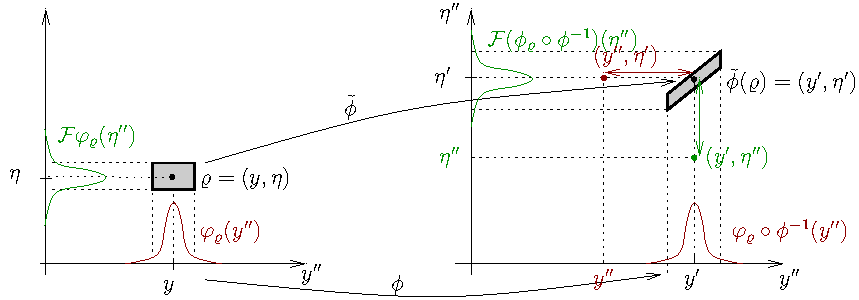
\includegraphics[scale=1]{figures/wave_packet-1.pdf} 
\caption{\label{fig:wave_packet}
Evolution of a wave packet $\varphi_{\varrho}$ in space and Fourier space. In Lemma~\ref{lem:Description-of-evolving}, the decay of the functions $(\varphi_{\varrho}\circ\phi^{-1})(y'')$ and $(\clF(\varphi_{\varrho}\circ\phi^{-1}))(\eta'')$ is controlled respectively from the distances $\Vert (y',\eta')-(y'',\eta')\Vert _{g_{\varrho}}$ and $\Vert (y',\eta')-(y',\eta'')\Vert _{g_{\varrho}}$.}
\end{figure}


\begin{proof}
We use the notations introduced in Lemma~\ref{lem:Description-of-evolving}. We have
\begin{multline*}
\left(\varphi_{\varrho}\circ\phi^{-1}\right)\left(y''\right)\underset{\eqref{eq:wave_packet}, \eqref{eq:def_phi_xi}, \eqref{eq:def_phi_0}}{=}\frac{1}{\left(2\pi\right)^{\left(n+1\right)/2}} \int_{\bbR^{n+1}}e^{i\eta''\left(\phi^{-1}\left(y''\right)-y\right)}\left(m\left(\eta''\right)\right)^{-1/2}\\
\exp\left(-\frac{1}{2}\left|\delta\left(\eta\right)\left(\eta''-\eta\right)\right|^{2}\right)d\eta''.
\end{multline*}
Let us consider the change of variable $\eta''\mapsto\tilde{\eta}''$ with
\[
\tilde{\eta}'':=\delta\left(\eta\right)\left(\eta''-\eta\right),
\]
giving
\begin{multline}\label{eq:wp-1}
\left(\varphi_{\varrho}\circ\phi^{-1}\right)\left(y''\right)  =\det \delta\left(\eta\right)^{-1}\left(2\pi\right)^{-\left(n+1\right)/2}e^{i\eta\left(\phi^{-1}\left(y''\right)-y\right)}
\\
\int_{\bbR^{n+1}}e^{i\tilde{\eta}''\delta\left(\eta\right)^{-1}\left(\phi^{-1}\left(y''\right)-y\right)}\left(m\left(\eta''\right)\right)^{-1/2}\exp\left(-\frac{1}{2}\left|\tilde{\eta}''\right|^{2}\right)d\tilde{\eta}''.
\end{multline}
From the following estimates that follows from~\eqref{eq:expression_m}, $\forall\alpha,\exists C_{\alpha}>0,\forall\eta\in\bbR^{n+1},$
\[
\partial_{\tilde{\eta}''}^{\alpha}\left(\left(m\left(\eta''\right)\right)^{-1/2}\exp\left(-\frac{1}{2}\left|\tilde{\eta}''\right|^{2}\right)\right)\leq C_{\alpha}\det \delta\left(\eta\right)^{1/2},
\]
and noticing that~\eqref{eq:wp-1} is a usual Fourier transform of a Schwartz function~\cite[p.~222]{taylor_tome1}, we deduce that $\forall N>0,\exists C_{N,t}>0,\forall\eta\in\bbR^{n+1}$,
\begin{align*}
\left|\left(\varphi_{\varrho}\circ\phi^{-1}\right)\left(y''\right)\right| & \leq\left(\det \delta\left(\eta\right)\right)^{-1/2}C_{N,t}\left\langle \left|\delta\left(\eta\right)^{-1}\left(\phi\left(y\right)-y''\right)\right|\right\rangle ^{-N}\\
& =\left(\det \delta\left(\eta\right)\right)^{-1/2}C_{N,t}\left\langle \left\Vert \tilde{\phi}\left(\varrho\right)-\left(y'',\eta'\right)\right\Vert _{g_{\varrho}}\right\rangle ^{-N}.
\end{align*}
This gives~\eqref{eq:size_wave_packet}. To show~\eqref{eq:F_phi_t}, we write
\begin{align*}
\left(\clF\left(\varphi_{\varrho}\circ\phi^{-1}\right)\right)\left(\eta''\right) & =\left(2\pi\right)^{-\left(n+1\right)/2}\int_{\bbR^{\left(n+1\right)}}e^{-i\eta''y''}\left(\varphi_{\varrho}\circ\phi^{-1}\right)\left(y''\right)dy''.
\end{align*}
We consider the change of variable $y''\mapsto\tilde{y}''$ with
\[
\tilde{y}'':=\delta\left(\eta\right)^{-1}\left(y''-\phi\left(y\right)\right),
\]
giving
\begin{multline*}
\left(\clF\left(\varphi_{\varrho}\circ\phi^{-1}\right)\right)\left(\eta''\right)\\
\underset{\eqref{eq:wp-1}}{=}\left(2\pi\right)^{-\left(n+1\right)}\int_{\bbR^{2\left(n+1\right)}}e^{if\left(\tilde{\eta}''',\tilde{y}''\right)}\left(m\left(\eta'''\right)\right)^{-1/2}\exp\left(-\frac{1}{2}\left|\tilde{\eta}'''\right|^{2}\right)d\tilde{\eta}'''d\tilde{y}'',
\end{multline*}
with phase function
\begin{align}
f\left(\tilde{\eta}''',\tilde{y}''\right) & :=-\eta''y''+\eta'''\left(\phi^{-1}\left(y''\right)-y\right).\label{eq:f_function}
\end{align}
In order to integrate by parts later, we first extract the linear part of the function $f$ at $(0,0)$, writing (beware that in our notations, partial derivative have multi-components $\partial_{\tilde{y}''}\equiv(\partial_{\tilde{x}_{j}''},\partial_{\tilde{z}''})$, $\partial_{\tilde{\eta}'''}\equiv(\partial_{\tilde{\xi}_{j}'''},\partial_{\tilde{\omega}'''})$ with $j=1\ldots n$)
\[
f\left(\tilde{\eta}''',\tilde{y}''\right)=f\left(0,0\right)+\tilde{\eta}'''.\partial_{\tilde{\eta}'''}f\left(0,0\right)+\tilde{y}''.\partial_{\tilde{y}''}f\left(0,0\right)+f_{\nonlin}\left(\tilde{\eta}''',\tilde{y}''\right),
\]
with
\begin{align*}
\partial_{\tilde{\eta}'''}f\left(\tilde{\eta}''',\tilde{y}''\right) &\underset{\eqref{eq:f_function}}{=}\left(\phi^{-1}\left(y''\right)-y\right)\delta\left(\eta\right)^{-1}.
\\
\partial_{\tilde{y}''}f\left(\tilde{\eta}''',\tilde{y}''\right) &\underset{\eqref{eq:f_function}}{=}\left(-\eta''+\eta'''\left(d\phi^{-1}\right)\left(y''\right)\right)\delta\left(\eta\right)
\end{align*}
hence
\[
\partial_{\tilde{\eta}'''}f\left(0,0\right)=0,\quad\partial_{\tilde{y}''}f\left(0,0\right)=\left(-\eta''+\eta\left(d\phi_{\phi\left(y\right)}^{-1}\right)\right)\delta\left(\eta\right).
\]
We get
\begin{multline}\label{eq:FexptX}
\left(\clF\left(\varphi_{\varrho}\circ\phi^{-1}\right)\right)\left(\eta''\right)\\
=\left(2\pi\right)^{-\left(n+1\right)}\det \delta\left(\eta\right)^{1/2}e^{if\left(0,0\right)}\int_{\bbR^{2\left(n+1\right)}}e^{i\tilde{y}''\partial_{\tilde{y}''}f\left(0,0\right)}u_{\varrho}\left(\tilde{\eta}''',\tilde{y}''\right)d\tilde{\eta}'''d\tilde{y}''
\end{multline}
with
\[
u_{\varrho}\left(\tilde{\eta}''',\tilde{y}''\right)=e^{if_{\nonlin}\left(\tilde{\eta}''',\tilde{y}''\right)}\det \delta\left(\eta\right)^{-1/2}\left(m\left(\eta'''\right)\right)^{-1/2}\exp\left(-\frac{1}{2}\left|\tilde{\eta}'''\right|^{2}\right).
\]
We have
\begin{align*}
\partial_{\tilde{\eta}'''}^{2}f\left(\tilde{\eta}''',\tilde{y}''\right)=0,\quad\partial_{\tilde{\eta}'''}\partial_{\tilde{y}''}f\left(\tilde{\eta}''',\tilde{y}''\right) &=\left(d\phi^{-1}\right)\left(y''\right),\\
\partial_{\tilde{y}''}^{2}f\left(\tilde{\eta}''',\tilde{y}''\right) &=\left(\eta'''\left(dd\phi^{-1}\right)\left(y''\right)\right)\delta\left(\eta\right)^{2}.
\end{align*}
In the flow direction $d_{z}\phi^{-1}=1$ so $dd_{z}\phi^{-1}=0$. Hence only $d_{x}d_{x}\phi^{-1}$ matters and we have
\[
\left\Vert \partial_{\tilde{y}''}^{2}f\left(0,\tilde{y}''\right)\right\Vert =\left\Vert \left(d_{x}d_{x}\phi^{-1}\right)\left(y''\right)\eta\left\langle \eta\right\rangle ^{-2\alpha^{\perp}}\right\Vert
\]
that is uniformly bounded with respect to $\varrho=(y,\eta)$ if and only if $\alpha^{\perp}\geq1/2$, that is condition~\eqref{eq:conditions}. We check that higher derivatives of $f$ are always uniformly bounded so we get that $u_{\varrho}(\tilde{\eta}''',\tilde{y}'')\in\clS(\bbR^{2(n+1)})$ is uniformly bounded with respect to $\varrho$. Since the Fourier transform sends the Schwartz space to itself continuously~\cite[p.~222]{taylor_tome1} we deduce that $\forall N>0,\exists C_{N,t}>0$,
\begin{align*}
\left|\clF\left(\varphi_{\varrho}\circ\phi^{-1}\right)\left(\eta''\right)\right| & \ineq{\ref{eq:FexptX}}\left(\det \delta\left(\eta\right)\right)^{1/2}C_{N,t}\left\langle \left|\left(-\eta''+\eta\left(d\phi_{\phi\left(y\right)}^{-1}\right)\right)\delta\left(\eta\right)\right|\right\rangle ^{-N}\\
&\mkern8mu =C_{N,t}\left(\det \delta\left(\eta\right)\right)^{1/2}\left\langle \left\Vert \tilde{\phi}\left(\varrho\right)-\left(y',\eta''\right)\right\Vert _{g_{\varrho}}\right\rangle ^{-N}.
\end{align*}
This gives~\eqref{eq:F_phi_t}.
\end{proof}

\subsubsection{\label{subsec:Resolution-of-identity-2}
Global wave packet transform}

We have defined the wave packet transform in a local chart. We next define a global wave packet transform on $C^{\infty}(M)$. Recall the notation $y=(x,z)\in\bbR^{n+1}$, $\eta=(\xi,\omega)\in\bbR^{n+1}$ and $\varrho=(y,\eta)\in\bbR^{2(n+1)}$ in~\eqref{eq:def_k_tilde_j}. For a chart index $j$, we write $\clB_{j}$ for the wave packet transform $\clB$ defined in~\eqref{eq:def_Bargamnn_B} acting on $C_{0}^{\infty}(V_{j})$ and set
\[
\clB:=\oplus_{j=1}^{J}\clB_{j}:\oplus_{j=1}^{J}C_{0}^{\infty}(V_{j})\rightarrow\oplus_{j=1}^{J}\clS\left(\bbR_{\varrho}^{2\left(n+1\right)}\right).
\]
The global wave packet transform that we will consider is essentially the composition
\begin{equation}\label{eq:B-I}
\clB\circ I=\oplus_{j=1}^{J}\clB_{j}\circ I_{j}:C^{\infty}\left(M\right)\rightarrow\oplus_{j=1}^{J}\clS\left(\bbR_{\varrho}^{2\left(n+1\right)}\right).
\end{equation}
But, in order to get a more geometric expression, we would like that each wave packet corresponds to a point on $T^{*}M$ (rather than a point in $\bbR_{\varrho}^{2(n+1)}$) and that the global wave packet transform sends a function on $M$ to a function on $T^{*}M$. Simultaneously, we would like to have an exact resolution of identity~\eqref{eq:resol_ident_Pi_rho}. Thus we define the global wave packet transform as follows.

Notice that for $u\in C^{\infty}(M)$, the component $(\clB_{j}I_{j})(u)$ will not be supported on a bounded subset in $\bbR_{\varrho}^{2(n+1)}$ though they decay rapidly on the outside of $\supp(\chi_{j})\times\bbR^{n+1}$. This is problematic for the purpose of getting the geometric expression mentioned above. Our solution to this problem is to consider a bijection $\tilde{\psi}$ from the space $T^{*}V_{j}$ to $\bbR_{\varrho}^{2(n+1)}=T^{*}\bbR^{n+1}$ so that it restricts to the identity map on a small neighborhood of $\supp(\chi_{j})\Subset V_{j}$. Recall the notation for local charts in~\eqref{eq:def_kappa_j} with the constant $c>0$. Let $\epsilon>0$ and
\[
V_{j,\epsilon}:=\text{\ensuremath{\bbB_{x}^{n}(c-\epsilon)}\ensuremath{\times}}\ensuremath{\bbB_{z}^{n}(l-\epsilon)}=\left\{ \left(x,z\right)\in\bbR^{n}\times\bbR;\,\left|x\right|<c-\epsilon\text{ and }\left|z\right|<l-\epsilon\right\} \subset V_{j}.
\]
We assume $\epsilon$ small enough so that $\supp(\chi_{j})\subset V_{j,\epsilon}$ for any $j$. We take a (surjective) diffeomorphism
\begin{equation}\label{eq:def_psi}
\psi:V_{j}\rightarrow\bbR_{y}^{n+1}
\end{equation}
such that
\begin{equation}\label{eq:psi_y_y}
\psi\left(y\right)=y\qquad\text{for }y\in V_{j,\epsilon/2}.
\end{equation}
We may and will assume that the Jacobian of $\psi$ has temperate growth, that is, for some $N_{0}>0$ and $C>0$,
\[
\left|\det d_{y}\psi\right|\leq C\left|\psi\left(y\right)\right|^{N_{0}}\quad\text{for all }y\in V_{j}
\]
and also that $\psi$ is expanding, that is,
\begin{equation}\label{eq:expand}
\left\Vert \psi\left(y\right)-\psi\left(y'\right)\right\Vert \geq\left\Vert y-y'\right\Vert \quad\text{for all }y,y'\in V_{j}.
\end{equation}
Then we consider the trivial extension of the map $\psi$ to $T^{*}V_{j}$, which is defined by
\begin{equation}\label{eq:def_psi_tilde}
\tilde{\psi}:\varrho=\left(y,\eta\right)\in T^{*}V_{j}\mapsto\varrho'=\left(\psi\left(y\right),\eta\right)\in T^{*}\bbR^{n+1}.
\end{equation}
Beware that this map $\tilde{\psi}$ differs from the canonical extension $d^{*}\psi^{-1}$ of $\psi$ to $T^{*}V_{j}$.
\vspace*{-6pt}
\begin{cBoxA}{}
\begin{defi}[Global wave packet transform $\clT$]\label{def:Phi_j_rho}
For $1\leq j\leq J$ and $\rho\in T^{*}U_{j}$, we define a wave packet function $\Phi_{\rho,j}\in C^{\infty}(U_{j})\subset C^{\infty}(M)$ on the local chart $U_{j}$ by
\begin{equation}\label{eq:def_wave_packet_Phi_j_rho}
\Phi_{\rho,j}(m):=\left|\det \left(d\psi\right)(\kappa_{j}(m))\right|^{1/2}\cdot\left(I_{j}^{\dagger}\varphi_{\tilde{\psi}\left(\tilde{\kappa}_{j}\left(\rho\right)\right)}\right)(m).
\end{equation}
Then we define the wave packet transform
\begin{equation}\label{eq:def_T_in-1}
\clT:
\begin{cases}
C^{\infty}\left(M;\bbC\right) & \rightarrow\clS\left(T^{*}M;\bbC^{J}\right)\\
u\left(m\right) & \mapsto v\left(\rho\right)=\left(\langle\Phi_{\rho,j}|u\rangle_{L^{2}\left(M\right)}\right)_{j\in\left\{ 1,2,\ldots J\right\} }
\end{cases}
\end{equation}
where we set $\Phi_{\rho,j}=0$ for $\rho\notin T^{*}U_{j}$.
\end{defi}
\end{cBoxA}
\vspace*{-6pt}
With the definitions above, we obtain the next proposition.
\vspace*{-5pt}
%%%%%%%%%%%%%%%%%%%%%%%%%%%%%%%%%%%%%%%
\begin{cBoxB}{}
\begin{prop}[Resolution of identity on $C^{\infty}(M)$]\label{prop:resolution_identity_CM}
The $L^{2}$-adjoint operator of $\clT$ is given by
\begin{equation}\label{eq:def_T_*}
\clT^{\dagger}:
\begin{cases}
\clS\left(T^{*}M;\bbC^{J}\right) & \rightarrow C^{\infty}\left(M;\bbC\right)\\
v\left(\rho\right) & \mapsto u\left(m\right)=\int_{\rho\in T^{*}M}\sum_{j}v_{j}\left(\rho\right)\Phi_{\rho,j}\left(m\right)\frac{d\rho}{\left(2\pi\right)^{n+1}}.
\end{cases}
\end{equation}
We have the following resolution of identity on $C^{\infty}\left(M\right)$:
\begin{align}\label{eq:resol_ident_Pi_rho}
\Id _{/C^{\infty}\left(M\right)} & =\clT^{\dagger}\clT=\int_{T^{*}M}\Pi\left(\rho\right)\frac{d\rho}{\left(2\pi\right)^{n+1}}
\end{align}
where
\begin{equation}\label{eq:Pi_(rho)}
\Pi\left(\rho\right):=\sum_{j=1}^{J}\Phi_{\rho,j}\langle\Phi_{\rho,j}|.\rangle_{L^{2}}.
\end{equation}
The last operator $\Pi(\rho)$ is a finite rank operator, self-adjoint and non-negative on $L^{2}(M,dm)$ and satisfies, $\forall\epsilon>0$,
\begin{equation}\label{eq:Tr(Pi_rho)}
\left|\Tr\left(\Pi\left(\rho\right)\right)-1\right|=O\left(\Delta^{1-\epsilon}\left(\rho\right)+\delta^{\parallel}\left(\eta\right)\right).
\end{equation}
and $\Vert \Pi(\rho\Vert _{\Tr_{L^{2}}}=\Tr(\Pi(\rho))$.
\end{prop}
\end{cBoxB}
%%%%%%%%%%%%%%%%%%%%%%%%%%%%%%%%%%%%%%%%%%%%%%%%%

\begin{rema}
Eq.\eqref{eq:resol_ident_Pi_rho} shows that $\clT:L^{2}(M;\bbC)\rightarrow L^{2}(T^{*}M;\bbC^{J})$ is an isometry, see Remark~\ref{rem:Projection}. A drawback of the previous construction is that $\Pi(\rho)$ is not rank one and $\Pi(\rho)^{2}\neq\Pi(\rho)$. This is inevitable because the wave packets for $\rho\in T^{*}M$ on different charts are not equal and the differences are not negligible.
\end{rema}


\begin{rema}
If $\alpha^{\parallel}<1-\alpha^{^{\perp}}$ then the right hand side of~\eqref{eq:Tr(Pi_rho)} is simply $O(\delta^{\parallel}(\eta))$, because we have $\Delta(\rho)\asymp\langle |\eta|\rangle^{-(1-\alpha^{\perp})}$ and $\delta^{\parallel}(\eta)\asymp\langle |\eta|\rangle ^{-\alpha^{\parallel}}$.
\end{rema}

\begin{proof}
We have
\begin{equation}\label{eq:res_id-1}
\begin{split}
\Id _{/C^{\infty}\left(M\right)} & \underset{\eqref{eq:I*_I},\eqref{eq:resol_identity_B}}{=}\left(\clB\circ I\right)^{\dagger}\circ\left(\clB\circ I\right)
\\
& \mkern16mu\underset{\eqref{eq:resol_identity_B}}{=}\sum_{j}\int_{\bbR^{2n+2}}I_{j}^{\dagger}\circ\pi\left(y',\eta'\right)\circ I_{j}\frac{dy'd\eta'}{\left(2\pi\right)^{n+1}}\\
& \mkern16mu\underset{\eqref{eq:def_psi}}{=}\sum_{j}\int_{\left(y,\eta\right)\in T^{*}V_{j}}I_{j}^{\dagger}\circ\pi\left(\psi\left(y\right),\eta\right)\circ I_{j}\left|\det \left(d\psi\left(y\right)\right)\right|\frac{dyd\eta}{\left(2\pi\right)^{n+1}} \\
& \mkern22mu=\int_{T^{*}M}\Pi\left(\rho\right)\frac{d\rho}{\left(2\pi\right)^{n+1}}\underset{
\eqref{eq:Pi_(rho)},\eqref{eq:def_T_in-1},\eqref{eq:def_T_*}}{=} \clT^{\dagger}\clT
\end{split}
\end{equation}
where, for $\rho\in T^{*}M$, $m=\pi(\rho)\in M$, we set
\begin{equation}\label{eq:Pi_rho}
\begin{split}
\Pi\left(\rho\right) &\mkern8mu{:=}\sum_{j\,;\,y\,\in\,U_{j}}\big|\det \left(d\psi\left(\kappa_{j}\left(m\right)\right)\right)\big|\cdot I_{j}^{\dagger}\circ\pi\left(\tilde{\psi}\left(\tilde{\kappa}_{j}\left(\rho\right)\right)\right)\circ I_{j}
\\
&\underset{\eqref{eq:def_wave_packet_Phi_j_rho}}{=}\sum_{j}\left|\Phi_{\rho,j}\right\rangle\left\langle\Phi_{\rho,j}|\cdot\right\rangle.
\end{split}
\end{equation}
The last operator $\Pi(\rho)$ is of finite rank and $L^{2}$-self-adjoint. Its trace is
\begin{equation}\label{eq:eq}
\Tr\left(\Pi\left(\rho\right)\right)\underset{\eqref{eq:Pi_rho},\eqref{eq:def_pi_wave_packet}}{=} \sum_{j\,;\,y\,\in \,U_{j}}\big|\det \left(d\psi\left(\kappa_{j}\left(m\right)\right)\right)\big|\left\langle\varphi_{\tilde{\psi}\left(\tilde{\kappa}_{j}\left(\rho\right)\right)}\,\middle|\,I_{j}I_{j}^{\dagger}\varphi_{\tilde{\psi}\left(\tilde{\kappa}_{j}\left(\rho\right)\right)}\right\rangle.
\end{equation}
On the right hand side, we have
\begin{align*}
\left\langle\varphi_{\tilde{\psi}\left(\tilde{\kappa}_{j}\left(\rho\right)\right)}\,\middle|\,I_{j}I_{j}^{\dagger}\varphi_{\tilde{\psi}\left(\tilde{\kappa}_{j}\left(\rho\right)\right)}\right\rangle & \underset{\eqref{eq:def_I*-2}}{=}\int_{y'\,\in\,\bbR^{n+1}}\chi_{j}^{2}\left(y'\right)\left|\det d\kappa_{j}\left(\kappa_{j}^{-1}\left(y'\right)\right)\right|\left|\varphi_{\tilde{\psi}\left(\tilde{\kappa}_{j}\left(\rho\right)\right)}\left(y'\right)\right|^{2}dy',\\
& \mkern6mu= \chi_{j}^{2}\left(\kappa_{j}\left(m\right)\right)\left|\det d\kappa_{j}\left(m\right)\right|\left\Vert \varphi_{\tilde{\psi}\left(\tilde{\kappa}_{j}\left(\rho\right)\right)}\right\Vert ^{2}+O\left(\delta^{\parallel}\left(\eta\right)\right)\\
& \mkern-18mu\underset{\eqref{eq:partition_quadratic_unity-1},\eqref{eq:norme_wave_packet}}{=} 1+O\left(\Delta^{1-\epsilon}\left(\rho\right)+\delta^{\parallel}\left(\eta\right)\right).
\end{align*}
The remainder $O(\delta^{\parallel}(\eta))$ in the second line comes from the size of wave packets along the flow direction and Taylor expansion of the smooth functions in the integral. We deduce~\eqref{eq:Tr(Pi_rho)}.
\end{proof}

\begin{cBoxB}{}
\begin{prop}[Wave packet projector]\label{lem:Bargmann projector}
The operator
\begin{equation}\label{eq:BargmannProjector}
\clP :=\clT\clT^{\dagger}:L^{2}\left(T^{*}M;\bbC^{J},\frac{d\rho}{\left(2\pi\right)^{n+1}}\right)\rightarrow L^{2}\left(T^{*}M;\bbC^{J},\frac{d\rho}{\left(2\pi\right)^{n+1}}\right)
\end{equation}
is the orthogonal projector on the image of $\clT$. It is called \emph{wave packet projector}. Its Schwartz kernel
\begin{equation}\label{eq:kernel_T_T*}
\langle\delta_{\rho',j'},|\clP \delta_{\rho,j}\rangle_{L^{2}\left(T^{*}M\right)}=\langle\Phi_{j',\rho'}|\Phi_{j,\rho}\rangle_{L^{2}\left(M\right)}
\end{equation}
decays rapidly on the outside the diagonal: for any $N\text{\ensuremath{\ge}0}$, there exists $C_{N}>0$ such that
\begin{equation}\label{eq:estimate_Bergman_kernel}
\left|\langle\delta_{\rho',j'}|\clP \delta_{\rho,j}\rangle_{L^{2}\left(T^{*}M\right)}\right|=\left|\langle\Phi_{j',\rho'}|\Phi_{j,\rho}\rangle_{L^{2}\left(M\right)}\right|\leq C_{N}\left\langle \dist_{g}\left(\rho',\rho\right)\right\rangle ^{-N}
\end{equation}
for any $\rho,\rho'\in T^{*}M$.
\end{prop}
\end{cBoxB}

\begin{proof}
For the former claim, we refer to Remark~\ref{rem:Projection}. The estimate~\eqref{eq:estimate_Bergman_kernel} is a consequence of~\eqref{eq:size_wave_packet}. (We will show a more general statement in Lemma~\ref{thm:Microlocality-of-the_TO}.)
\end{proof}

\subsection{Pseudo-differential operators}\label{subsec:Pseudo-differential-operator}

\subsubsection{Pseudo-differential operators (PDO)}

In this section we use the family of operators $\Pi(\rho)$ in~\eqref{eq:Pi_(rho)} to define pseudo-differential operators on $C^{\infty}(M)$.

\begin{cBoxA}{}
\begin{defi}[Pseudo-differential operator $\Opp(a)$]\label{def:Op}
Let $a\in L_{\locc }^{\infty}(T^{*}M)$ whose growth at infinity is temperate in the sense that, for some constant $C>0$ and $N\ge0$, we have
\begin{equation}\label{eq:symbol_temperate}
\left|a\left(\rho\right)\right|\le C\langle\left|\rho\right|\rangle^{N}\quad\text{for all }\rho\in T^{*}M.
\end{equation}
For such a function $a$, we define the pseudo-differential operator (PDO) with the symbol $a$
\[
\Opp\left(a\right):C^{\infty}\left(M\right)\to C^{\infty}\left(M\right)
\]
by
\begin{equation}\label{eq:def_operator}
\Opp\left(a\right){:=}\int_{T^{*}M}a\left(\rho\right)\Pi\left(\rho\right)\frac{d\rho}{\left(2\pi\right)^{n+1}}\underset{\eqref{eq:Pi_(rho)},\eqref{eq:def_T_in-1},\eqref{eq:def_T_*}}{=}\clT^{\dagger}\clM_{a}\clT
\end{equation}
where $\clM_{a}:\clS(T^{*}M;\bbC^{J})\rightarrow\clS(T^{*}M;\bbC^{J})$ denotes the component-wise multiplication by $a$, that is, $\clM_{a}v(\rho)=a(\rho)v(\rho)$. We have $\Opp(1)\underset{\eqref{eq:resol_ident_Pi_rho}}{=}\Id $.
\end{defi}
\end{cBoxA}

\begin{rema}
The quantization formula~\eqref{eq:def_operator} is usually called anti-Wick quantization~\cite[Defi.~1.7.3]{nicola_rodino_livre_11} or Toeplitz quantization~\cite[Chap.~13.4]{zworski_book_2012} (or Wick quantization in~\cite[Chap.~2.4.1]{lerner2011metrics}) or coherent states quantization. The function $a$ is called the (anti-Wick) symbol of the operator $\Opp(a)$.
\end{rema}


\begin{rema}
From Remark~\ref{rem:As-in-}, for $u,v\in C^{\infty}(M)$, we have $\clT u,\clT v\in\clS(T^{*}M)$ and
\[
\langle u|\Opp\left(a\right)v\rangle_{L^{2}\left(M\right)}\underset{\eqref{eq:def_operator}}{=}\left\langle\left(\clT u\right)\overline{\left(\clT v\right)}\,\middle|\,a\right\rangle_{L^{2}\left(T^{*}M\right)},
\]
we deduce that the map $\Opp:a\in L_{\locc}^{\infty}(T^{*}M)\mapsto\Opp(a)$ defined in~\eqref{eq:def_operator} can be extended to symbols $a$ that are a tempered distribution:
\[
\Opp:
\begin{cases}
\clS'\left(T^{*}M\right) & \rightarrow L\left(\clS\left(M\right),\clS'\left(M\right)\right)\\
a & \mapsto\Opp\left(a\right)
\end{cases},
\]
where $L(\clS(M),\clS'(M))$ stands for linear operators from $\clS(M)$ to $\clS'(M)$.
\end{rema}

\begin{cBoxB}{}
\begin{prop}[Basic properties of PDO]\label{prop:We-havewhere-}
If $a\in L^{\infty}(T^{*}M)$, the operator $\Opp(a)$ extends to a bounded operator on $L^{2}(M)$ and we have
\begin{equation}
\left\Vert \Opp \left(a\right)\right\Vert _{L^{2}\left(M\right)}\underset{}{\leq}\left|a\right|_{L^{\infty}\left(T^{*}M\right)}.\label{eq:norme_symbol}
\end{equation}
If $a\in L^{1}(T^{*}M)$, the operator $\Opp (a)$ extends to a trace class operator on $L^{2}(M)$ whose trace is given by
\begin{equation}
\Tr\left(\Opp \left(a\right)\right)\underset{\eqref{eq:def_operator}}{=}\int a\left(\rho\right)\Tr\left(\Pi\left(\rho\right)\right)\frac{d\rho}{\left(2\pi\right)^{n+1}}\label{eq:Tr_Opa}
\end{equation}
and whose trace norm is bounded as $\forall\epsilon>0$,
\begin{equation}
\left\Vert \Opp \left(a\right)\right\Vert _{\Tr}\underset{\eqref{eq:Tr(Pi_rho)}}{\leq}\left\Vert a\left(\rho\right)\left(1+O\left(\Delta^{1-\epsilon}\left(\rho\right)+\delta^{\parallel}\left(\rho\right)\right)\right)\right\Vert _{L^{1}\left(T^{*}M\right)}.\label{eq:norm_Tr_Op}
\end{equation}
\end{prop}
\end{cBoxB}

\begin{proof}
The former claim on the operator norm follows from Lemma~\ref{lem:Bargmann projector} and the expression~\eqref{eq:Prop_Opa}. (See the proof of Theorem~\ref{thm:Composition-of-PDO.} where we detail this and prove a more general statement.) The latter claims on the trace norm are consequences of the expression~\eqref{eq:def_operator} and the estimate~\eqref{eq:Tr(Pi_rho)}.
\end{proof}
\begin{rema}
From~\eqref{eq:norme_symbol} it is natural to consider the norm $L^{\infty}(T^{*}M)$ on symbols space so that the linear operator $\Opp :L^{\infty}(T^{*}M)\rightarrow\clL(L^{2}(M),L^{2}(M))$ is bounded. We will use this to derive expressions as in~\eqref{eq:res1}.
\end{rema}


\begin{rema}
We can write the PDO $\Opp (a)$ more explicitly by using local charts as
\begin{equation}\label{eq:Prop_Opa}
\Opp \left(a\right)=\left(\clB I\right)^{\dagger}\clM_{\tilde{a}}\left(\clB I\right)
\end{equation}
where $\clM_{\tilde{a}}$ denotes the component-wise multiplication on $\oplus_{j=1}^{J}\bbR_{\varrho}^{2(n+1)}$ by functions $\tilde{a}=(\tilde{a}_{j})_{1\,\le\,j\,\le\,J}$ where $\tilde{a}_{j}:T^{*}\bbR^{n+1}\to\bbC$ is the function $a$ viewed in the local chart $\tilde{\psi}\circ\tilde{\kappa}_{j}:T^{*}U_{j}\to T^{*}\bbR^{n+1}$:
\begin{equation}\label{eq:def_a_tilde_j}
\tilde{a}_{j}\left(\varrho'\right)=a\left(\tilde{\kappa}_{j}^{-1}\left(\tilde{\psi}^{-1}\left(\varrho'\right)\right)\right)\quad\text{for }\varrho'\in T^{*}\bbR^{n+1}.
\end{equation}
Indeed, recalling the definitions of the operator $\clB$ in~\eqref{eq:def_Bargamnn_B}, we have
\end{rema}
\begin{equation}\label{eq:Op_a}
\begin{split}
\Opp \left(a\right) & =\int_{T^{*}M}a\left(\rho\right)\Pi\left(\rho\right)\frac{d\rho}{\left(2\pi\right)^{n+1}}
\\
& \mkern-10mu\underset{\eqref{eq:Pi_(rho)}}{=}\sum_{j}\int a\left(\tilde{\kappa}_{j}^{-1}\left(\varrho\right)\right)\left|\det \left(d\psi\left(y\right)\right)\right|I_{j}^{\dagger}\pi\left(\tilde{\psi}\left(\varrho\right)\right)I_{j}\frac{d\varrho}{\left(2\pi\right)^{n+1}} \\
& \mkern-10mu\underset{\eqref{eq:def_psi_tilde}}{=}\sum_{j}\int_{\bbR^{2n+2}}a\left(\tilde{\kappa}_{j}^{-1}\left(\tilde{\psi}^{-1}\left(\varrho'\right)\right)\right)I_{j}^{\dagger}\pi\left(\varrho'\right)I_{j}\frac{dy'd\eta}{\left(2\pi\right)^{n+1}} \\
& =\left(\clB I\right)^{\dagger}\clM_{\tilde{a}}\left(\clB I\right)
\end{split}
\end{equation}
where $\varrho=(y,\eta)\in T^{*}V_{j}$ and $\varrho'=(y',\eta)=\tilde{\psi}(\varrho)\in T^{*}\bbR^{n+1}$.

\subsubsection{The Sobolev spaces \texorpdfstring{$\clH _{W}(M)$}{HW(M)}}\label{subsec:Sobolev-space}

Next we define generalized Sobolev spaces $\clH _{W}(M)$ from a weight function $W\in C(T^{*}M;\bbR^{+})$ for which we put the following assumption.

\begin{cBoxA}{}
\begin{defi}[Temperate weight function]\label{def:temperate_W-1}
We consider a family of strictly positive continuous functions $W_{h_{0}}\in C(T^{*}M;\bbR^{+})$ that depends on parameter $h_{0}>0$. This family is said to be $(C_{W},N_{W})$-\emph{temperate} for some constants $C_{W}\geq1,N_{W}>0$ if for every $h_{0}>0$ small enough, we have
\begin{multline}\label{eq:temperate_property-W-2}
\frac{W_{h_{0}}\left(\rho'\right)}{W_{h_{0}}\left(\rho\right)}\leq C_{W}\left\langle h_{0}\,\dist_{g}\left(\rho',\rho\right)\right\rangle ^{N_{W}}
\\
\text{for every }\rho,\rho'\in T^{*}U_{j}\text{ and }1\le j\le J.
\end{multline}
For simplicity we will write $W=W_{h_{0}}$. Let us write the unit co-sphere bundle for the metric $g_{M}$ on $M$ by $S^{*}M:=\{ \rho\in T^{*}M;\,\Vert \rho\Vert _{g_{M}}=1\} $. Then the \emph{order function} $r_{W}:S^{*}M\to\bbR$ of $W$ is the function that expresses the (upper) growth rate of the function $W$ in each direction and defined precisely by
\begin{equation}\label{eq:def_order-2}
r_{W}\left(\rho\right):=\inf\left\{ r\in\bbR\:\mid\exists C>0,\forall\alpha>1,W\left(\alpha\rho\right)\leq C\alpha^{r}\right\}.
\end{equation}
\end{defi}
\end{cBoxA}

\begin{rema}
The temperate property of $W$ implies that the function $r_{W}$ is bounded.
\end{rema}


\begin{rema}\label{rem:h0-model}
The role of the small parameter $h_{0}$ in~\eqref{eq:temperate_property-W-2} is somehow to assume that the function $W$ is flat with respect to the metric (or with respect to the size of wave packets). Here is a simple toy model to show how we will use this parameter $h_{0}$ technically. Let $x\in\bbR$, $A(x)=e^{-x^{2}}$, $W_{h_{0}}(x):=\langle h_{0}x\rangle ^{N_{W}}$ and
\[
I\left(h_{0},N_{W}\right):=\int_{\bbR}A\left(x\right)W_{h_{0}}\left(x\right)dx.
\]
We have for fixed $h_{0}>0$ that $I(h_{0},N_{W})\underset{N_{W}\,\rightarrow\,+\infty}{\rightarrow}+\infty$. However, from the estimate $\forall N,\exists C_{N},\forall x|A(x)|\leq C_{N}\langle x\rangle ^{-N}$ and $\Vert A(x)\Vert _{L^{1}}\leq C$, we deduce that
\begin{equation}
\exists C>0,\forall N_{W}>0,\exists h_{0}>0,\quad\left|I\left(h_{0},N_{W}\right)\right|\leq C.\label{eq:est}
\end{equation}
\begin{proof}
To show~\eqref{eq:est}, we split the integral in two parts: (1) $|x|\leq h_{0}^{-1}$ where $W_{h_{0}}(x){\asymp}1$ and $\int_{|x|\leq h_{0}^{-1}}A(x)W(x)dx\leq C$ independent on $N_{W},h_{0}$ and (2) $|x|\geq h_{0}^{-1}$, where
\begin{align*}
\int_{\left|x\right|\,\geq\,h_{0}^{-1}}A\left(x\right)W\left(x\right)dx & \leq C_{N}h_{0}^{N_{W}}\int_{\left|x\right|\geq h_{0}^{-1}}\left|x\right|^{N_{W}-N}dx\\
& \leq\frac{C_{N}h_{0}^{N_{W}}}{N-N_{W}-1}h_{0}^{-N_{W}+N-1}=\frac{C_{N}}{N-N_{W}-1}h_{0}^{N-1},
\end{align*}
for some large $N>N_{W}+1$. We finally take $h_{0}$ small enough.
\end{proof}
\end{rema}



We define the Sobolev spaces $\clH _{W}(M)$ as follows. This definition is similar to the definition of Sobolev spaces in micro-local analysis given in~\cite[Defi.2.6.1]{lerner2011metrics} or~\cite[Section~1.7.4]{nicola_rodino_livre_11}.

\begin{cBoxA}{}
\begin{defi}[The Sobolev space $\clH _{W}(M)$]\label{def:Anisotropic_Sob_space}
Let $W\in C(T^{*}M;\bbR^{+})$ be a temperate function~\eqref{eq:temperate_property-W-2} called weight function. For $u,v\in C^{\infty}(M)$, we define the $\clH _{W}$-scalar product by
\begin{equation}\label{eq:def_H_W_M}
\begin{split}
\left\langle u|v\right\rangle _{\clH _{W}}
&{:=}\left\langle u\,\middle|\,\Opp \left(W^{2}\right)v\right\rangle _{L^{2}\left(M,dm\right)}\\
&\mkern-8mu\underset{\eqref{eq:Op_a}}{=}\big\langle\clM_{W}\clT u\,\big|\,\clM_{W}\clT v\big\rangle_{L^{2}\left(T^{*}M,\frac{d\rho}{\left(2\pi\right)^{n+1}}\right)}.
\end{split}
\end{equation}
The associated $\clH _{W}$-norm is defined by
\begin{align}\label{eq:def_Sobolev_norm}
\left\Vert u\right\Vert _{\clH _{W}}^{2}:=\langle u|u\rangle_{\clH _{W}} & =\left\Vert \clM_{W}\clT u\right\Vert _{L^{2}\left(T^{*}M\right)}^{2}.
\end{align}
The Sobolev space $\clH _{W}(M)$ is defined as the Hilbert space obtained by completion of $C^{\infty}(M)$ with respect to the norm~\eqref{eq:def_Sobolev_norm}:
\begin{equation}\label{eq:def_H_W}
\clH _{W}\left(M\right):=\overline{C^{\infty}\left(M\right)}^{\left\Vert.\right\Vert _{\clH _{W}}}.
\end{equation}
\end{defi}
\end{cBoxA}

By definition we have the isometric embedding
\begin{equation}\label{eq:isometry}
\clM_{W}\clT\,:\,\clH _{W}\left(M\right)\rightarrow L^{2}\left(T^{*}M;\bbC^{J}\right).
\end{equation}
We have
\[
H^{r_{\max}}\left(M\right)\subset\clH _{W}\left(M\right)\subset H^{r_{\min}}\left(M\right)
\]
where $H^{r}(M)$ denotes the usual Sobolev space of constant order $r\in\bbR$~\cite[Chap.3]{taylor_tome1} and $r_{\max}:=\max_{S^{*}M}r_{W}$, $r_{\min}:=-\max_{S^{*}M}r_{W^{-1}}$ with the order function $r_{W}$ defined in Definition~\ref{def:temperate_W-1}. In particular, if $W\equiv1$, we have $\Vert u\Vert _{W}=\Vert u\Vert _{L^{2}(M)}$ and $\clH _{W}(M)=L^{2}(M)$ from~\eqref{eq:res_id-1}.

\subsubsection{How to estimate the operator norm using Schur Lemma}

We give here a general remark about a way (very common in microlocal analysis) to estimate the operator norm $\Vert B\Vert _{\clH _{W}}$ of a given operator $B:\clH _{W}(M)\rightarrow\clH _{W}(M)$. We consider the commutative diagram:
\begin{equation}\label{eq:lift_diagram-1}
\begin{CD}\clH _{W}\left(M\right)@>{B}>>\clH _{W}\left(M\right)\\
@V{\clM_{W}\clT}VV@V{\clM_{W}\clT}VV\\
L^{2}\left(T^{*}M;\bbC^{J}\right)@>{B_{W}}>>L^{2}\left(T^{*}M;\bbC^{J}\right)
\end{CD}
\end{equation}
where $B_{W}$ denotes the lifted operator defined by
\begin{equation}\label{eq:def_BW}
B_{W}:=\clM_{W}\clT B\clT^{\dagger}\clM_{W^{-1}}.
\end{equation}
From~\eqref{eq:isometry}, $\clM_{W}\clT$ is an isometric embedding and $\clM_{W}^{\dagger}=\clM_{W^{-1}}$, hence $\Vert \clM_{W}\clT\Vert\linebreak =1$, $\Vert \clT^{\dagger}\clM_{W^{-1}}\Vert =\Vert (\clM_{W}\clT)^{\dagger}\Vert =1$ and the operator norm of $B$ on $\clH _{W}(M)$ is equal to that of $B_{W}$ on $L^{2}(T^{*}M;\bbC^{J})$ (recall Remark~\ref{rem:Projection}.):
\begin{equation}\label{eq:compare_norms}
\left\Vert B\right\Vert _{\clH _{W}}=\left\Vert B_{W}\right\Vert _{L^{2}\left(T^{*}M\,;\,\bbC^{J}\right)}.
\end{equation}
We can estimate $\Vert B_{W}\Vert _{L^{2}(T^{*}M;\bbC^{J})}$ from its Schwartz kernel
\[
\left\langle\delta_{\rho',j'}\,\middle|\,B_{W}\delta_{\rho,j}\right\rangle=\left\langle\delta_{\rho',j'}\,\middle|\,\clT B\clT^{\dagger}\delta_{\rho,j}\right\rangle\frac{W\left(\rho'\right)}{W\left(\rho\right)}
\]
and using Schur Lemma:

\begin{cBoxB}{}
\begin{lemm}[Schur Lemma]\label{lem:Schur-Lemma-.}
\cite[Lemma~2.8.4, p.~50]{martinez-01}.
\begin{multline}\label{eq:schur_lemma}
\left\Vert B_{W}\right\Vert _{L^{2}\left(T^{*}M;\bbC^{J}\right)} \leq
\\
 \left(\sup_{\rho',j'}\sum_{j}\int\left|\left\langle\delta_{\rho',j'}\,\middle|\,B_{W}\delta_{\rho,j}\right\rangle\right|d\rho\right)^{1/2}\left(\sup_{\rho,j}\sum_{j'}\int\left|\left\langle\delta_{\rho',j'}\,\middle|\,B_{W}\delta_{\rho,j}\right\rangle\right|d\rho'\right)^{1/2}.
\end{multline}
\end{lemm}
\end{cBoxB}

\begin{rema}\label{rem:To-estimate-the}
To estimate the trace norm $\Vert B\Vert _{\Tr_{\clH _{W}}}=\Vert B_{W}\Vert _{\Tr_{L^{2}}}$ we note that the operator $B$ is written as an integral of rank one operators:
\begin{equation}\label{eq:expression_integral_of_rankone}
\begin{split}
B &\underset{\eqref{eq:def_BW}}{=}  \clT^{\dagger}W^{-1}B_{W}W\clT
\\
& \mkern10mu= \sum_{j,j'}\int\left\langle\delta_{\rho',j'}\,\middle|\,B_{W}\delta_{\rho,j}\right\rangle\cdot\frac{W\left(\rho\right)}{W\left(\rho'\right)}\cdot\left|\Phi_{\rho',j'}\right\rangle\,\left\langle\Phi_{\rho,j}\,\middle|.\,\right\rangle_{L^{2}}\frac{d\rho'}{\left(2\pi\right)^{n+1}}\frac{\text{d\ensuremath{\rho}}}{\left(2\pi\right)^{n+1}}
\end{split}
\end{equation}
and $\Vert |\Phi_{\rho',j'}\rangle\langle\Phi_{\rho,j}|.\rangle_{L^{2}}\Vert _{\Tr_{\clH _{W}}}=\Vert \Phi_{\rho,j}\Vert _{\clH _{W}}^{2}\leq C$ uniformly.
\end{rema}


\subsubsection{Description of the vector field \texorpdfstring{$X$}{X} by a PDO}\label{subsec:Description-of-the}

We first introduce a definition that will be used to express that some operator $R$ is ``under control'' or ``negligible'' in our analysis. It will means that the Schwartz kernel of $\clT R\clT^{\dagger}$ decays very fast outside the diagonal graph of $\tilde{\phi}^{t}$ defined in~\eqref{eq:lifted_flow} and moreover that on the graph, the Schwartz kernel is bounded by a given positive function $h(\rho)$.

\begin{cBoxA}{}
\begin{defi}\label{def:Let--be-1}
Let $t\in\bbR$ and a positive function $h:\rho\in T^{*}M\rightarrow h(\rho)\in\bbR^{+}$. We define $\Psi_{\tilde{\phi}^{t}}(h)$ as the set of operators $R:\clS(M)\rightarrow\clS'(M)$ such that for any $N>0$, there exists a constant $C_{N,t}>0$ such that for any $\rho,\rho'\in T^{*}M$
\begin{equation}\label{eq:microl_estimate-2}
\left|\langle\delta_{\rho'}|\clT R\clT^{\dagger}\delta_{\rho}\rangle_{L^{2}\left(T^{*}M\right)}\right| \leq C_{N,t}\left\langle \dist_{g}\left(\rho',\tilde{\phi}^{t}\left(\rho\right)\right)\right\rangle ^{-N}h\left(\rho\right).
\end{equation}
In particular for $t=0$, we simply write $\Psi(h):=\Psi_{\tilde{\phi}^{t}}(h)$.
\end{defi}
\end{cBoxA}

\begin{rema}
$h$ is defined up to constant scaling i.e. for any $C>0$,
\[
\Psi_{\tilde{\phi}^{t}}\left(h\right)=\Psi_{\tilde{\phi}^{t}}\left(Ch\right).
\]
\end{rema}

\begin{cBoxB}{}
\begin{prop}[Principal symbol of the vector field $X$]\label{prop:We-havewith-a}
We have
\begin{equation}
-X=\Opp \left(i\boldsymbol{\omega}\right)+R\label{eq:symbol_X}
\end{equation}
with a remainder $R\in\Psi(\langle |\rho|\rangle ^{\alpha^{\parallel}})$, where $\boldsymbol{\omega}$ denotes the frequency function~\eqref{eq:omega_function} and $0\leq\alpha^{\parallel}<1$ is a parameter for the metric $g$ along the flow direction in~\eqref{eq:conditions}.
\end{prop}
\end{cBoxB}

\begin{proof}
For $\rho'\in T^{*}M$, we put $\omega'=\boldsymbol{\omega}(\rho')$. Since $(-X)=\frac{\partial}{\partial z}$ in flow box coordinates, we check from~\eqref{eq:def_wave_packet_Phi_j_rho} and~\eqref{eq:wave_packet} (or the asymptotic expression~\eqref{eq:wave_packet_1}) that $\forall N>0,\exists C_{N}>0$,$\forall\rho,\rho'$,$\forall j,j'$,
\begin{multline}\label{eq:X_omega}
\big|\left\langle\Phi_{\rho',j'}\,\middle|\,\left(-X-i\omega'\right)\Phi_{\rho,j}\right\rangle\big|\\
=\big|\left\langle\left(-X-i\omega'\right)\Phi_{\rho',j'}\,\middle|\,\Phi_{\rho,j}:\right\rangle\big|\leq\delta^{\parallel}\left(\rho\right)^{-1}C_{N}\left\langle \dist_{g}\left(\rho',\rho\right)\right\rangle^{-N},
\end{multline}
where $\delta^{\parallel}(\rho)^{-1}\eq{\ref{eq:def_delta}}\langle |\rho|\rangle ^{\alpha^{\parallel}}$.
\end{proof}

\begin{rema}
The error term $R$ in~\eqref{eq:symbol_X} dominates the principal term on the domain $\rho=(\xi,\omega)\in T^{*}M\text{ s.t. }|\xi|^{\alpha^{\parallel}}\geq\omega$.
\end{rema}


\subsubsection{Continuity theorem for PDO}

The next theorems are a variant of standard theorem for PDO, called continuity theorem and composition theorem. We state and prove them here for the PDO's that we have defined in~\eqref{eq:def_operator}.

Recall that in the definition~\eqref{eq:temperate_property-W-2} of temperate property of the weight $W$, there are two parameters $N_{W},h_{0}$. In the next Theorem, we obtain a bound for the operator norm $\Vert \Opp (a)\Vert _{\clH _{W}(M)\,\rightarrow\,\clH _{W}(M)}$. This bound can be uniform with respect to $N_{W}$ if $h_{0}>0$ is chosen small enough accordingly.

\begin{cBoxB}{}
\begin{theo}[Continuity theorem]\label{thm:Continuity-of-PDO}
Suppose that $W$ is $(C_{W},N_{W})$-temperate according to property~\eqref{eq:temperate_property-W-2}. Then there exists a constant $C>0$ such that for any bounded measurable function $a\in L^{\infty}(T^{*}M)$, the PDO $\Opp (a)$ extends to a bounded operator on $\clH _{W}(M)$ with the following estimate
\[
\left\Vert \Opp (a)\right\Vert _{\clH _{W}(M)\,\rightarrow\,\clH _{W}(M)}\leq C\|a\|_{L^{\infty}}.
\]
Moreover, $C$ may depend on $C_{W}$ but not on $N_{W}$ if $h_{0}$ is taken small enough.
\end{theo}
\end{cBoxB}

\begin{proof}
We write
\begin{align*}
\left(\Opp \left(a\right)\right)_{W}&\underset{\eqref{eq:def_BW}}{=} W\clP \clM_{a}\clP W^{-1}
\\
\intertext{So}
\left\langle\delta_{\rho'}\,\middle|\, \left(\Opp \left(a\right)\right)_{W}\delta_{\rho}\right\rangle &\mkern8mu=\frac{W\left(\rho'\right)}{W\left(\rho\right)}\int\left\langle\delta_{\rho'}\,\middle|\,\clP \delta_{\rho_{1}}\right\rangle a\left(\rho_{1}\right)\langle\delta_{\rho_{1}}|\clP \delta_{\rho}\rangle\frac{d\rho_{1}}{\left(2\pi\right)^{n+1}},
\end{align*}
and $\forall N>0,\exists C_{N}>0,$
\begin{multline*}
\left|\langle\delta_{\rho'}\,\middle|\,\left(\Opp \left(a\right)\right)_{W}\delta_{\rho}\rangle\right|\\
\begin{aligned}
&\mkern-10mu\underset{\eqref{eq:temperate_property-W-2},\eqref{eq:estimate_Bergman_kernel}}{\leq}\mkern-25mu C_{W}\left\langle h_{0}\,\dist_{g}\left(\rho',\rho\right)\right\rangle ^{N_{W}}C_{N}\mkern-5mu
\int\left\langle \dist_{g}\left(\rho',\rho_{1}\right)\right\rangle ^{-N}\left|a\left(\rho_{1}\right)\right|\left\langle \dist_{g}\left(\rho_{1},\rho\right)\right\rangle ^{-N}\mkern-8mu\frac{d\rho_{1}}{\left(2\pi\right)^{n+1}}\\
&\mkern15mu\leq  C_{W}\left\langle h_{0}\,\dist_{g}\left(\rho',\rho\right)\right\rangle ^{N_{W}}C_{N}\|a\|_{L^{\infty}}\left\langle \dist_{g}\left(\rho',\rho\right)\right\rangle ^{-N}
\end{aligned}
\end{multline*}
If $h_{0}\dist_{g}(\rho',\rho)\leq1$ then $\forall N>0,\exists C_{N}>0,$
\[
\left|\langle\delta_{\rho'}|\left(\Opp \left(a\right)\right)_{W}\delta_{\rho}\rangle\right|\leq C_{W}C_{N}\|a\|_{L^{\infty}}\left\langle \dist_{g}\left(\rho',\rho\right)\right\rangle ^{-N}
\]
with $C_{N}$ independent on $N_{W}$. If $h_{0}\dist_{g}(\rho',\rho)\geq1$ then
\begin{equation}\label{eq:aide}
\begin{split}
\left\langle h_{0}\,\dist_{g}\left(\rho',\rho\right)\right\rangle ^{N_{W}}C_{N}\left\langle \dist_{g}\left(\rho',\rho\right)\right\rangle ^{-N} & \asymp C_{N}h_{0}^{N_{W}}\left\langle \dist_{g}\left(\rho',\rho\right)\right\rangle ^{-N+N_{W}}
\\
& =C_{N'}\left\langle \dist_{g}\left(\rho',\rho\right)\right\rangle ^{-N'},
\end{split}
\end{equation}
with $N'=N-N_{W}$ and $C_{N'}=C_{N}h_{0}^{N_{W}}$. If we take $h_{0}$ small enough with respect to $N_{W}$ we get again $\forall N'>0,\exists C_{N'}>0,$
\[
\left|\left\langle\delta_{\rho'}\,\middle|\,\left(\Opp \left(a\right)\right)_{W}\delta_{\rho}\right\rangle\right|\leq C_{W}C_{N'}\|a\|_{L^{\infty}}\left\langle \dist_{g}\left(\rho',\rho\right)\right\rangle ^{-N'}
\]
with $C_{N'}$ independent on $N_{W}$. Finally, by Schur Lemma~\ref{lem:Schur-Lemma-.} we conclude that the operator norm of $\Opp (a)_{W}$ in $L^{2}$ is bounded by $C\|a\|_{L^{\infty}}$ and the same holds true for $\Opp (a)$ in $\clH _{W}(M)$, where $C$ depends on $C_{W}$ but does not depend on $N_{W}$, and $h_{0}>0$ has been taken small enough depending on $N_{W}$.
\end{proof}

\subsubsection{Composition theorem for PDO}

\begin{cBoxA}{}
\begin{defi}\label{def:Let--be}
Let $h\in C(T^{*}M;\bbR^{+})$ be some continuous function, let $N_{0}\geq0$ and $0<h_{0}<1$. A bounded measurable function $b\in L^{\infty}(T^{*}M)$ is said to be $(h,N_{0},h_{0})$-\emph{slowly varying symbol with respect to the metric} $g$ if
\begin{equation}\label{eq:slow_variations}
\left|b\left(\rho'\right)-b\left(\rho\right)\right|\leq h\left(\rho\right)\,\left\langle h_{0}\,\dist_{g}\left(\rho',\rho\right)\right\rangle ^{N_{0}}\quad\text{for all }\rho,\rho'\in T^{*}M.
\end{equation}
\end{defi}
\end{cBoxA}

\begin{rema}
The small parameter $h_{0}$ will be used in Lemma~\ref{lem:For-the-weight}. Recall Remark~\ref{rem:h0-model} about the usefulness of a similar small parameter $h_{0}$.
\end{rema}

The following lemma will be useful in the proof of the composition Theorem~\ref{thm:Composition-of-PDO.} below. Recall $\clP =\clT\clT^{\dagger}$ defined in~\eqref{eq:BargmannProjector}.

\begin{cBoxB}{}
\begin{lemm}[Basic Lemma for slow varying symbols]\label{lem:Basic_Lemma}
Assume that $b\in C(T^{*}M)$ satisfies the slow variation property~\eqref{eq:slow_variations} with a function $h$ and some parameters $N_{0},h_{0}>0$. Then the Schwartz kernel of the operator $[\clM_{b},\clP ]=\clM_{b}\clP -\clP \clM_{b}$ satisfies $\forall N,\exists C_{N}>0,\exists h_{0}>0$, $\forall\rho',\rho\in T^{*}M,\forall j,j'\in\{1,\,\ldots J\} $,
\begin{equation}\label{eq:commut_P}
\left|\left\langle\delta_{\rho',j'}\,\middle|\,\left[\clM_{b},\clP \right]\delta_{\rho,j}\right\rangle\right|\leq C_{N}h\left(\rho\right)\left\langle \dist_{g}\left(\rho',\rho\right)\right\rangle ^{-N}.
\end{equation}
Using the notation of Definition~\ref{def:Let--be-1}, we can write that $[\clM_{b},\clP ]\in\Psi(h)$.
\end{lemm}
\end{cBoxB}

\begin{proof}
We have
\[
\left\langle\delta_{\rho',j'}\,\middle|\,\left[\clM_{b},\clP \right]\delta_{\rho,j}\right\rangle=\left\langle\delta_{\rho',j'}\,\middle|\,\clP \delta_{\rho,j}\right\rangle\left(b\left(\rho'\right)-b\left(\rho\right)\right)
\]
Hence $\forall N>0,\exists C_{N}>0$,
\begin{align*}
\left|\left\langle\delta_{\rho',j'}\,\middle|\,\left[\clM_{b},\clP \right]\delta_{\rho,j}\right\rangle\right|&\underset{(\eqref{eq:estimate_Bergman_kernel},\eqref{eq:slow_variations})}{\leq}  C_{N}h\left(\rho\right)\left\langle \dist_{g}\left(\rho',\rho\right)\right\rangle ^{-N}\left\langle h_{0}\,\dist_{g}\left(\rho',\rho\right)\right\rangle ^{N_{0}}
\\
&\mkern30mu\leq  C_{N}h\left(\rho\right)\left\langle \dist_{g}\left(\rho',\rho\right)\right\rangle ^{-N}.
\end{align*}
For the last line we proceed as in~\eqref{eq:aide} with $h_{0}$ small enough.
\end{proof}

\begin{rema}
In following Lemma and Theorems we will still have ``uniform estimates w.r.t. $N_{W}$,$N_{0}$'' in the sense of letting $h_{0}>0$ be small depending on $N_{W},N_{0}>0$ (as in Theorem~\ref{thm:Continuity-of-PDO}), and for this, we will use the shorter notation ``$\exists C>0,\forall N_{W},N_{0}>0,\exists h_{0}>0$''.
\end{rema}

%%%%%%%%%%%%%%%%%%%%%%%%%%%%%%%%%%%%%%%%%%%%
%\begin{cBoxA}{}
\begin{tcolorbox}[enhanced, frame style={purple!80}, interior style={red!0},breakable]
\begin{theo}[Composition theorem]\label{thm:Composition-of-PDO.}

For a bounded measurable function $a\in L^{\infty}(T^{*}M)$ and slowly varying symbol $b\in L^{\infty}(T^{*}M)$ as~\eqref{eq:slow_variations} with function $h$ and parameters $N_{0},h_{0}>0$, let us consider the operator
\[
B:=\Opp \left(a\right)\Opp \left(b\right)-\Opp \left(ab\right).
\]
For the Schwartz kernel of the corresponding lifted operator $B_{W}=\clM_{W}\clT B\clT^{\dagger}\clM_{W^{-1}}$ as defined in~\eqref{eq:def_BW} with parameter $N_{W}$ in~\eqref{eq:temperate_property-W-2}, we have $\forall N>0,\exists C_{N}>0,\forall N_{W},N_{0}>0,\exists h_{0}>0$, $\forall\rho',\rho\in T^{*}M,\forall j,j'\in\{ 1,\,\ldots J\} $,
\[
\left|\left\langle\delta_{\rho',j'}\,\middle|\,B_{W}\delta_{\rho,j}\right\rangle\right|\leq C_{N}\left|a\left(\rho\right)\right|h\left(\rho\right)\left\langle \dist_{g}\left(\rho',\rho\right)\right\rangle^{-N}.
\]
Using the notation of Definition~\ref{def:Let--be-1}, we can write that $B_{W}\in\Psi(|a|h)$. Consequently $\exists C>0,\forall N_{W},N_{0}>0,\exists h_{0}>0$,
\begin{enumerate}
\item If $\Vert ah\Vert _{L^{\infty}}<\infty$, we have
\begin{equation}\label{eq:norm_Compos_PDO}
\left\Vert B\right\Vert _{\clH _{W}}\leq C\left\Vert ah\right\Vert _{L^{\infty}}.
\end{equation}
\item If $\Vert ah\Vert _{L^{1}}<\infty$, the difference $\Opp (a)\circ\Opp (b)-\Opp (ab)$ is a trace class operator on $\clH _{W}(M)$ and we have
\[
\left\Vert B\right\Vert _{\Tr_{\clH _{W}}}\leq C\left\Vert ah\right\Vert _{L^{1}}.
\]
\end{enumerate}
These claims hold if we exchange $\Opp (a)$ and $\Opp (b)$ in the definition of $B$.
\end{theo}
\end{tcolorbox}
%\end{cBoxA}
%%%%%%%%%%%%%%%%%%%%%%%%%%%%%%%%%%%%%

\begin{proof}
We write
\[
B_{W}\eq{\ref{eq:def_BW}}W\clP \clM_{a}\left(\clP \clM_{b}-\clM_{b}\clP \right)\clP W^{-1}
\]
So (we omit chart indices $j,j'$ for simplicity)
\begin{multline*}
\left\langle\delta_{\rho'}\,\middle|\,B_{W}\delta_{\rho}\right\rangle\\ =\frac{W\left(\rho'\right)}{W\left(\rho\right)}\int\left\langle\delta_{\rho'}\,\middle|\,\clP \delta_{\rho_{1}}\right\rangle a\left(\rho_{1}\right)\left\langle\delta_{\rho_{1}}\,\middle|\,\left[\clP ,\clM_{b}\right]\delta_{\rho_{2}}\right\rangle \left\langle\delta_{\rho_{2}}\,\middle|\,\clP \delta_{\rho}\right\rangle\frac{d\rho_{1}}{\left(2\pi\right)^{n+1}}\frac{d\rho_{2}}{\left(2\pi\right)^{n+1}},
\end{multline*}
and
\begin{multline*}
\left|\langle\delta_{\rho'}|B_{W}\delta_{\rho}\rangle\right|\\
\begin{aligned}
&\mkern-70mu\underset{\eqref{eq:temperate_property-W-2},\eqref{eq:estimate_Bergman_kernel},\eqref{eq:slow_variations},\eqref{eq:commut_P}}{\leq}  C_{W}\left\langle h_{0}\,\dist_{g}\left(\rho',\rho\right)\right\rangle ^{N_{W}}C_{N}\int\left\langle \dist_{g}\left(\rho',\rho_{1}\right)\right\rangle ^{-N}\\
& \quad\left|a\left(\rho_{1}\right)\right|h\left(\rho_{1}\right)\left\langle \dist_{g}\left(\rho_{1},\rho_{2}\right)\right\rangle ^{-N}\left\langle \dist_{g}\left(\rho_{2},\rho\right)\right\rangle ^{-N}\frac{d\rho_{1}}{\left(2\pi\right)^{n+1}}\frac{d\rho_{2}}{\left(2\pi\right)^{n+1}},\\
&\leq C_{W}C_{N}\left|a\left(\rho\right)\right|h\left(\rho\right)\left\langle \dist_{g}\left(\rho',\rho\right)\right\rangle ^{-N}
\end{aligned}
\end{multline*}
In the last line, $h_{0}$ is chosen small enough with respect to $N_{W},N_{0}$. We obtain Item~1 by Schur Lemma~\ref{lem:Schur-Lemma-.} and Item~2 using Remark~\ref{rem:To-estimate-the}.
\end{proof}

The following corollary will be used in Section~\ref{par:Contribution} and can be skipped for the moment.

\begin{cBoxB}{}
\begin{coro}\label{cor:B3}
Let $\Omega_{R}$ be a compact subset on $T^{*}M$ which depends on a parameter $R\ge1$. Let $\boldsymbol{1}_{\Omega_{R}}:T^{*}M\rightarrow\{ 0,1\} $ the characteristic function of $\Omega_{R}$. Assume that $b_{R}:T^{*}M\rightarrow\bbC$ is a measurable function that takes constant value $1$ on the $R-$neighborhood of $\Omega_{R}$, that is,
\[
b_{R}\left(\rho'\right)=1\quad\text{whenever }\; \dist_{g}\left(\rho',\rho\right)\leq R \,\text{for}\, \ensuremath{\rho\in\Omega_{R}} \,\text{and}\, \ensuremath{\rho'\in T^{*}M}.
\]
Assume further that the growth of $b_{R}$ on the outside of $\Omega_{R}$ is temperate uniformly in $R$ in the sense that there exists $N_{0}>0$ and $C_{0}>0$ independent of the parameter $R$ such that $\forall\rho',\rho\in T^{*}M$,
\[
\left|b_{R}\left(\rho'\right)-b_{R}\left(\rho\right)\right|\leq C_{0}\left\langle \dist_{g}\left(\rho',\rho\right)\right\rangle ^{N_{0}}.
\]
Then, for arbitrarily large $N>0$, there exists a constant $C_{N,W}>0$ such that for any $R\geq1$,
\begin{equation}\label{eq:corollary_compos}
\left\Vert \Opp \left(b_{R}\right)\circ\Opp \left(\boldsymbol{1}_{\Omega_{R}}\right)-\Opp \left(\boldsymbol{1}_{\Omega_{R}}\right)\right\Vert _{\clH _{W}}\leq C_{N,W}R^{-N}.
\end{equation}
\end{coro}
\end{cBoxB}

\begin{proof}
Let us check first that, for arbitrarily large $N>0$, we have
\[
\left|b_{R}\left(\rho'\right)-b_{R}\left(\rho\right)\right|\leq C_{0}R^{-N}\dist_{g}\left(\rho',\rho\right)^{N_{0}+N}\quad\text{for all \ensuremath{\rho\in\Omega_{R}} and }\rho'\in T^{*}M.
\]
This is trivial if $\dist_{g}(\rho',\rho)\leq R$ because $b_{R}(\rho')=b_{R}(\rho)=1$. If $\dist_{g}(\rho',\rho)\geq R\geq1$, we have
\[
\left|b_{R}\left(\rho'\right)-b_{R}\left(\rho\right)\right|\leq C_{0}\dist_{g}\left(\rho',\rho\right)^{N_{0}}\leq C_{0}R^{-N}\dist_{g}\left(\rho',\rho\right)^{N+N_{0}},
\]
so this is true again. Now we apply Theorem~\ref{thm:Composition-of-PDO.} with setting $a=\boldsymbol{1}_{\Omega_{R}}$, $b=b_{R}$ and $h\equiv R^{-N}$. Since $\Opp (ab)=\Opp (\boldsymbol{1}_{\Omega_{R}}b_{R})=\Opp (\boldsymbol{1}_{\Omega_{R}})$ and $\Vert ah\Vert _{L^{\infty}}=\Vert \boldsymbol{1}_{\Omega_{R}}h\Vert _{L^{\infty}}=R^{-N}$, we obtain the conclusion~\eqref{eq:corollary_compos}.
\end{proof}

\subsection{Properties of the transfer operator}

In this section we consider the transfer operator $\clL^{t}=\exp(tA)$ with $A=-X+V$ defined in~\eqref{eq:def_Transfer_operator}. As we noted at the beginning of this section, we will assume only that $X$ is a smooth non-singular vector field on $M$ and $V$ is some smooth complex valued function on $M$.

\subsubsection{The matrix elements of the transfer operator between wave packets}\label{subsec:A-matrix-elements}

The next theorem is rather a direct consequence of Lemma~\ref{lem:Description-of-evolving}. It shows that the Schwartz kernel of the lifted operator $\clT\clL^{t}\clT^{\dagger}$ (i.e. the matrix elements of the transfer operator $\clL^{t}$ expressing transformation between wave-packets)
\begin{equation}\label{eq:Schwartz_kernel_transfer_op}
\left\langle\delta_{\rho',j'}\,\middle|\,\clT\clL^{t}\clT^{\dagger}\delta_{\rho,j}\right\rangle_{L^{2}\left(T^{*}M\right)}\underset{\eqref{eq:def_T_*}}{=}\left\langle\Phi_{\rho',j'}\,\middle|\,\clL^{t}\Phi_{\rho,j}\right\rangle_{L^{2}\left(M\right)}
\end{equation}
is (micro-)localized around the graph of the flow map $\tilde{\phi}^{t}$ in $T^{*}M$, Eq.\eqref{eq:lifted_flow}, with respect to the distance $\dist_{g}\left(\cdot,\cdot\right)$.

\begin{cBoxB}{}
\begin{theo}[Propagation of singularities by the transfer operator $\clL^{t}$]\label{thm:Microlocality-of-the_TO}
For any $t\in\bbR$ and any $N>0$, there exists a constant $C_{N,t}>0$ such that
\begin{equation}\label{eq:microl_estimate}
\left|\left\langle\delta_{\rho',j'}\,\middle|\,\clT\clL^{t}\clT^{\dagger}\delta_{\rho,j}\right\rangle_{L^{2}\left(T^{*}M\right)}\right| \leq C_{N,t}\left\langle \dist_{g}\left(\rho',\tilde{\phi}^{t}\left(\rho\right)\right)\right\rangle ^{-N}
\end{equation}
for any $\rho,\rho'\in T^{*}M$ and $0\leq j,j'\leq J$. Using the notation of Definition~\ref{def:Let--be-1}, we can write that $\clL^{t}\in\Psi_{\tilde{\phi}^{t}}(1)$.
\end{theo}
\end{cBoxB}

\begin{proof}
Let $t\geq0$ and $\rho,\rho'\in T^{*}M$. We take $0\leq j,j'\leq J$ such that $m=\pi(\rho)\in U_{j}$ and $m'=\pi(\rho')\in U_{j'}$ respectively. In the following we will sometimes omit the indices $j$ and $j'$ from the notation. Set
\[
\varrho=\left(y,\eta\right)=\tilde{\psi}\left(\tilde{\kappa}_{j}\left(\rho\right)\right),\quad\varrho'=\left(y',\eta'\right)=\tilde{\psi}\left(\tilde{\kappa}_{j'}\left(\rho'\right)\right)\quad\in T^{*}\bbR^{n+1}
\]
where $\tilde{\kappa}_{j}$ is defined in~\eqref{eq:def_k_tilde_j} and $\tilde{\psi}$ is defined in~\eqref{eq:def_psi_tilde}. We write the Schwartz kernel~\eqref{eq:Schwartz_kernel_transfer_op} as
\begin{multline}\label{eq:kernel}
\left\langle\delta_{\rho',j'}\,\middle|\,\clT\clL^{t}\clT^{\dagger}\delta_{\rho,j}\right\rangle_{L^{2}\left(T^{*}M\right)}\\
\underset{\eqref{eq:def_wave_packet_Phi_j_rho}}{=}\big|\det \big(d\psi\left(\kappa_{j'}\left(m'\right)\right)\big)\big|^{1/2}\big|\det \big(d\psi\left(\kappa_{j}\left(m\right)\right)\big)\big|^{1/2}\left\langle\varphi_{\varrho'}\,\middle|\,\left(I_{j'}\clL^{t}I_{j}^{\dagger}\right)\varphi_{\varrho}\right\rangle_{L^{2}}.
\end{multline}
Below we estimate the last term
\begin{equation}\label{eq:def_K}
K\left(\varrho',\varrho\right):=\left\langle\varphi_{\varrho'}\,\middle|\,\left(I_{j'}\clL^{t}I_{j}^{\dagger}\right)\varphi_{\varrho}\right\rangle_{L^{2}}.
\end{equation}
We assume that $\phi^{t}(U_{j})\cap U_{j'}\neq\emptyset$ because the Schwartz kernel vanishes otherwise. Let
\[
\phi:=\kappa_{j'}\circ\phi^{t}\circ\kappa_{j}^{-1}\quad:\kappa_{j}\left(U_{j}\cap\phi^{-t}\left(U_{j'}\right)\right)\rightarrow\kappa_{j'}\left(\phi^{t}\left(U_{j}\right)\cap U_{j'}\right).
\]
For $u\in\clS(\bbR_{y}^{n+1})$, we have for $y''\in\bbR^{n+1}$,
\begin{equation}
\left(I_{j'}\clL^{t}I_{j}^{\dagger}u\right)\left(y''\right)\underset{\eqref{eq:def_Transfer_operator}}{=}Y\left(y''\right)u\left(\phi^{-1}\left(y''\right)\right)\label{eq:def_Ltilde-1}
\end{equation}
where $Y:\bbR^{n+1}\to\bbR$ is a $C^{\infty}$ function written precisely as
\[
Y\left(y''\right)=e^{V_{\left[-t,0\right]}\left(\kappa_{j'}^{-1}\left(y''\right)\right)}\chi_{j'}\left(y''\right)\chi_{j}\left(\phi^{-1}\left(y''\right)\right).
\]
The definition of the function $Y(.)$ is rather complicated but we only need the property that it is $C^{\infty}$ function supported on a compact subset $\supp\chi_{j'}$. We have
\begin{align}\label{eq:integrale}
K\left(\varrho',\varrho\right) \underset{\eqref{eq:def_K},\eqref{eq:def_Ltilde-1}}{=}\int_{\bbR^{n+1}}\overline{\varphi_{\varrho'}\left(y''\right)}\varphi_{\varrho}\left(\phi^{-1}\left(y''\right)\right)\,Y\left(y''\right)dy''.
\end{align}
We first bound this integral ``in space'' and use~\eqref{eq:size_wave_packet}, getting that $\forall N>0,\exists C_{N,t}>0,\forall\varrho,\varrho'\in T^{*}\bbR^{n+1}$,
\begin{align}
\left|K\left(\varrho',\varrho\right)\right| & \ineq{\ref{eq:integrale}}\int_{\bbR^{n+1}}\left|\overline{\varphi_{\varrho'}\left(y''\right)}\right|\left|\varphi_{\varrho}\left(\phi^{-1}\left(y''\right)\right)\right|\left|Y\left(y''\right)\right|dy''\label{eq:integrale-1}
\\
& \ineq{\ref{eq:size_wave_packet}}\left(\det \delta\left(\eta'\right)\right)^{-1/2}\left(\det \delta\left(\eta\right)\right)^{-1/2}C_{N,t}\nonumber\\
& \qquad\int_{\bbR^{n+1}}\left\langle \delta\left(\eta'\right)^{-1}\left(y'-y''\right)\right\rangle ^{-N}\left\langle \delta\left(\eta\right)^{-1}\left(\phi^{t}\left(y\right)-y''\right)\right\rangle ^{-N}dy''\label{eq:integrand}\nonumber
\end{align}
Let $\delta_{\max}:=\max\{\delta(\eta),\delta(\eta')\} $ and
\[
q:=\delta_{\max}^{-1}y'',a:=\delta_{\max}^{-1}y',b:=\delta_{\max}^{-1}\phi^{t}\left(y\right)
\]

giving
\begin{multline*}
\left|K\left(\varrho',\varrho\right)\right|\\\leq\left(\det \delta\left(\eta'\right)\right)^{-1/2}\left(\det \delta\left(\eta\right)\right)^{-1/2}\left(\det \delta_{\max}\right)C_{N,t}\int_{\bbR^{n+1}}\left\langle \left|q-a\right|\right\rangle ^{-N}\left\langle \left|q-b\right|\right\rangle ^{-N}dq
\end{multline*}
We split the integral:
\begin{multline*}
\int_{\bbR^{n+1}}\left\langle \left|q-a\right|\right\rangle ^{-N}\left\langle \left|q-b\right|\right\rangle ^{-N}dq\\
\leq\int_{q\in\bbR^{n+1},\left|q-a\right|\leq\left|q-b\right|} \left\langle \left|q-b\right|\right\rangle ^{-N}dq+\int_{q\in\bbR^{n+1},\left|q-a\right|\geq\left|q-b\right|}\left\langle \left|q-a\right|\right\rangle ^{-N}dq.
\end{multline*}
Let $D:=\frac{1}{2}|a-b|$. Since $\{ q\in\bbR^{n+1},|q-a|\leq|q-b|\} \subset\{ q\in\bbR^{n+1},|q-b|\geq D\}$, we have for $D\geq1$, $\exists C,C',C''>0\forall N$,
\begin{multline*}
\int_{q\,\in\,\bbR^{n+1},\left|q-a\right|\,\leq\,\left|q-b\right|}\left\langle \left|q-b\right|\right\rangle ^{-N}dq\\
\begin{aligned}
& \leq\int_{q\,\in\,\bbR^{n+1},\left|q-b\right|\,\geq\,D}\left\langle \left|q-b\right|\right\rangle ^{-N}dq=\int_{q\,\in\,\bbR^{n+1},\left|q\right|\,\geq\,D}\left\langle \left|q\right|\right\rangle ^{-N}dq\\
& \leq C\int_{r>D}r^{-N+n}dr\leq C'D^{-N+n+1}\leq C''\left\langle \left|a-b\right|\right\rangle ^{-N+n+1}.
\end{aligned}
\end{multline*}

Hence
\begin{align*}
\int_{\bbR^{n+1}}\left\langle \left|q-a\right|\right\rangle ^{-N}\left\langle \left|q-b\right|\right\rangle ^{-N}dq & \leq C\left\langle \left|a-b\right|\right\rangle ^{-N+n+1}\\
& \leq C\left\langle \left|\delta_{\max}^{-1}\left(y'-\phi^{t}\left(y\right)\right)\right|\right\rangle ^{-N+n+1}.
\end{align*}
Let $(y_{t},\eta_{t}):=\tilde{\phi}^{t}(\varrho)$. Using~\eqref{eq:equivalence_distance} we deduce that $\forall N>0,\exists C_{N,t}>0,\forall\varrho,\varrho'\in T^{*}\bbR^{n+1}$,
\begin{equation}\label{eq:K1}
\left|K\left(\varrho',\varrho\right)\right|\leq C_{N,t}\left\langle \left\Vert \tilde{\phi}^{t}\left(\varrho\right)-\left(y',\eta_{t}\right)\right\Vert _{g_{\varrho}}\right\rangle ^{-N}.
\end{equation}

Secondly we can write and bound the same integral~\eqref{eq:integrale} in Fourier space:
\[
K\left(\varrho',\varrho\right)\underset{\eqref{eq:def_K},\eqref{eq:def_Ltilde-1}}{=}\int_{\bbR^{n+1}}\overline{\left(\clF\varphi_{\varrho'}\right)\left(\eta''\right)}\clF\left(Y.\varphi_{\varrho}\circ\phi^{-1}\right)\left(\eta''\right)d\eta''
\]
and using~\eqref{eq:F_phi_t}, we deduce similarly that $\forall N>0,\exists C_{N,t}>0,\forall\varrho,\varrho'\in T^{*}\bbR^{n+1}$,
\begin{equation}
\left|K\left(\varrho',\varrho\right)\right|\leq C_{N,t}\left\langle \left\Vert \tilde{\phi}^{t}\left(\varrho\right)-\left(y_{t},\eta'\right)\right\Vert _{g_{\varrho}}\right\rangle ^{-N}.\label{eq:K2}
\end{equation}
Finally we write
\begin{align*}
\tilde{\phi}^{t}\left(\varrho\right)-\varrho' & =\tilde{\phi}^{t}\left(\varrho\right)-\left(y',\eta_{t}\right)+\left(y',\eta_{t}\right)-\left(y',\eta'\right)\\
& =\tilde{\phi}^{t}\left(\varrho\right)-\left(y',\eta_{t}\right)+\left(y_{t},\eta_{t}\right)-\left(y_{t},\eta'\right)\\
& =\left(\tilde{\phi}^{t}\left(\varrho\right)-\left(y',\eta_{t}\right)\right)+\left(\tilde{\phi}^{t}\left(\varrho\right)-\left(y_{t},\eta'\right)\right)
\end{align*}
and from~\eqref{eq:K1}, \eqref{eq:K2} we deduce that $\forall N>0,\exists C_{N,t}>0,\forall\varrho,\varrho'\in T^{*}\bbR^{n+1}$,
\[
\left|K\left(\varrho',\varrho\right)\right|\leq C_{N,t}\left\langle \left\Vert \tilde{\phi}^{t}\left(\varrho\right)-\varrho'\right\Vert _{g_{\varrho}}\right\rangle ^{-N}.
\]
Finally, from~\eqref{eq:kernel}, properties of the map $\tilde{\psi}$ in~\eqref{eq:def_psi_tilde} and using~\eqref{eq:log_log}, we obtain~\eqref{eq:microl_estimate}.
\end{proof}

\subsubsection{Egorov's Theorem on evolution of PDO.}

The results of this section are direct consequences of Theorem~\ref{thm:Microlocality-of-the_TO}. This first basic lemma will be used later.

\begin{cBoxB}{}
\begin{lemm}[Basic Egorov's Lemma for slow varying symbols]\label{lem:Basic_Egorov_lemma}
Assume that $a\in C(T^{*}M;\bbC)$ satisfies the slow variation property~\eqref{eq:slow_variations} with function $h$ and parameters $N_{0},h_{0}>0$. Then the Schwartz kernel of the operator
\[
R:=\clT\clL^{t}\clT^{\dagger}\clM_{a\circ\tilde{\phi}^{t}}-\clM_{a}\clT\clL^{t}\clT^{\dagger}
\]
satisfies $\forall N,\exists C_{N,t}>0,\forall N_{0}>0,\exists h_{0}>0,\forall\rho',\rho\in T^{*}M,\forall j,j'\in\{ 1,\,\ldots J\},$
\begin{equation}\label{eq:Egorov_Lemma}
\left|\langle\delta_{\rho',j'}|R\delta_{\rho,j}\rangle\right|\leq h\left(\rho'\right)C_{N,t}\left\langle \dist_{g}\left(\rho',\tilde{\phi}^{t}\left(\rho\right)\right)\right\rangle ^{-N}.
\end{equation}
\end{lemm}
\end{cBoxB}

\begin{proof}
We have
\begin{align*}
\left\langle\delta_{\rho',j'}\,\middle|\,R\delta_{\rho,j}\right\rangle & =\left\langle\delta_{\rho',j'}\,\middle|\,\clT\clL^{t}\clT^{\dagger}\delta_{\rho,j}\right\rangle\left(a\left(\tilde{\phi}^{t}\left(\rho\right)\right)-a\left(\rho'\right)\right)
\end{align*}
and hence
\begin{align*}
\left|\langle\delta_{\rho',j'}|R\delta_{\rho,j}\rangle\right| & \underset{\eqref{eq:microl_estimate},\eqref{eq:slow_variations}}{\leq}h\left(\rho'\right)C_{N,t}\left\langle \dist_{g}\left(\rho',\tilde{\phi}^{t}\left(\rho\right)\right)\right\rangle ^{-N}\left\langle h_{0}\dist_{g}\left(\rho',\tilde{\phi}^{t}\left(\rho\right)\right)\right\rangle ^{N_{0}}\\
& \mkern28mu\leq h\left(\rho'\right)C'_{N,t}\left\langle \dist_{g}\left(\rho',\tilde{\phi}^{t}\left(\rho\right)\right)\right\rangle ^{-N}
\end{align*}
For the last line we proceed as in~\eqref{eq:aide} with $h_{0}$ small enough.
\end{proof}

The next theorem concerns the operator $e^{-tX}$ that is the transport part of the transfer operator $\clL^{t}=e^{t(-X+V)}$. We will use this theorem later in the proof of Lemma~\ref{lem:bounded_resolvent_of_A'}.

%\begin{cBoxB}{}
\begin{tcolorbox}[enhanced, frame style={teal!80}, interior style={cyan!0}, breakable]
\begin{theo}[Egorov's Theorem]\label{thm:Egorov.-For-any}
Assume that $a\in C(T^{*}M;\bbC)$ is a slowly varying symbol (Eq. \eqref{eq:slow_variations} with parameters $N_{0},h_{0}>0$). Let us consider the operator
\[
B:=e^{-tX}\Opp \left(a\circ\tilde{\phi}^{t}\right)-\Opp \left(a\right)e^{-tX}.
\]
For the Schwartz kernel of the corresponding lifted operator $B_{W}=\clM_{W}\clT B\clT^{\dagger}\clM_{W^{-1}}$ as defined in~\eqref{eq:def_BW} with parameter $N_{W}$ in~\eqref{eq:temperate_property-W-2}, we have $\forall t\in\bbR,\forall N>0,\exists C_{N,t}>0,\forall N_{W},N_{0}>0,\exists h_{0}>0$, $\forall\rho',\rho\in T^{*}M,\forall j,j'\in\{ 1,\,\ldots J\} $,
\[
\left|\langle\delta_{\rho',j'}|B_{W}\delta_{\rho,j}\rangle\right|\leq C_{N,t}\frac{W\left(\tilde{\phi}^{t}\left(\rho\right)\right)}{W\left(\rho\right)}h\left(\tilde{\phi}^{t}\left(\rho\right)\right)\left\langle \dist_{g}\left(\rho',\tilde{\phi}^{t}\left(\rho\right)\right)\right\rangle ^{-N}
\]
Using the notation of Definition~\ref{def:Let--be-1}, we can write that $B\in\Psi_{\tilde{\phi}^{t}}(h)$. Consequently $\forall t\in\bbR,\exists C_{t}>0,\forall N_{W},N_{0}>0,\exists h_{0}>0$,
\begin{equation}\label{eq:norm_Egorov_PDO}
\left\Vert B\right\Vert _{\clH _{W}}\leq C_{t}\left\Vert \frac{W\circ\tilde{\phi}^{t}}{W}\cdot h\right\Vert _{L^{\infty}}
\end{equation}
and
\begin{equation}\label{eq:Egorov_Trace}
\left\Vert B\right\Vert _{\Tr_{\clH _{W}}}\leq C_{t}\left\Vert \frac{W\circ\tilde{\phi}^{t}}{W}\cdot h\right\Vert _{L^{1}}
\end{equation}
provided that the norm on the right-hand side is bounded in the respective inequality.
\end{theo}
\end{tcolorbox}
%\end{cBoxB}

\begin{proof}
We set
\[
R:=\clT e^{-tX}\clT^{\dagger}\clM_{a\circ\tilde{\phi}^{t}}-\clM_{a}\clT e^{-tX}\clT^{\dagger},
\]
and
\[
B_{W}:=\left(e^{-tX}\Opp \left(a\circ\tilde{\phi}^{t}\right)-\Opp \left(a\right)e^{-tX}\right)_{W}\eq{\ref{eq:def_BW}}, W\clP R\clP W^{-1}
\]
We will omit chart indices $j,j'$ for simplicity. We have
\begin{multline*}
\left\langle\delta_{\rho'}\,\middle|\,B_{W}\delta_{\rho}\right\rangle \\
 =\frac{W\left(\rho'\right)}{W\left(\tilde{\phi}^{t}\left(\rho\right)\right)}\frac{W\left(\tilde{\phi}^{t}\left(\rho\right)\right)}{W\left(\rho\right)}\int\left\langle\delta_{\rho'}\,\middle|\,\clP \delta_{\rho_{1}}\right\rangle\left\langle\delta_{\rho_{1}}\,\middle|\,R\delta_{\rho_{2}}\right\rangle\left\langle\delta_{\rho_{2}}\,\middle|\,\clP \delta_{\rho}\right\rangle\frac{d\rho_{1}}{\left(2\pi\right)^{n+1}}\frac{d\rho_{2}}{\left(2\pi\right)^{n+1}}
\end{multline*}
and
\begin{multline*}
\left|\langle\delta_{\rho'}|B_{W}\delta_{\rho}\rangle\right|\\
\begin{aligned}
&\underset{\eqref{eq:temperate_property-W-2},\eqref{eq:estimate_Bergman_kernel},\eqref{eq:slow_variations},\eqref{eq:Egorov_Lemma}}{\leq}  \mkern-10mu\frac{W\left(\tilde{\phi}^{t}\left(\rho\right)\right)}{W\left(\rho\right)}C_{W}\left\langle h_{0}\,\dist_{g}\left(\rho',\tilde{\phi}^{t}\left(\rho\right)\right)\right\rangle ^{N_{W}}C_{N,t}\int\left\langle \dist_{g}\left(\rho',\rho_{1}\right)\right\rangle ^{-N}\\
&\mkern95mu h\left(\rho_{1}\right)\left\langle \dist_{g}\left(\rho_{1},\tilde{\phi}^{t}\left(\rho_{2}\right)\right)\right\rangle ^{-N}  \left\langle h_{0}\,\dist_{g}\left(\rho_{1},\tilde{\phi}^{t}\left(\rho_{2}\right)\right)\right\rangle ^{N_{0}}\\
&\mkern140mu \left\langle \dist_{g}\left(\rho_{2},\rho\right)\right\rangle ^{-N}\frac{d\rho_{1}}{\left(2\pi\right)^{n+1}}\frac{d\rho_{2}}{\left(2\pi\right)^{n+1}}\\
&\mkern65mu\leq C_{W} C_{N,t}\frac{W\left(\tilde{\phi}^{t}\left(\rho\right)\right)}{W\left(\rho\right)}h\left(\tilde{\phi}^{t}\left(\rho\right)\right)\left\langle \dist_{g}\left(\rho',\tilde{\phi}^{t}\left(\rho\right)\right)\right\rangle ^{-N}.
\end{aligned}
\end{multline*}
In the last line, $h_{0}$ is chosen small enough with respect to $N_{W},N_{0}$. We deduce~\eqref{eq:norm_Egorov_PDO} using Schur Lemma~\ref{lem:Schur-Lemma-.} and also~\eqref{eq:Egorov_Trace} from Remark~\ref{rem:To-estimate-the}.
\end{proof}

\subsubsection{Strong continuity of the one-parameter group of transfer operators}\label{subsec:Strongly-continuous-semi-group}

In the next Lemma we show strong continuity of the transfer operator (this is version 1). Later in Lemma~\ref{lem:For-the-weight}, with additional properties on the escape function $W$ we will get some improved estimates (version 2).

\begin{cBoxB}{}
\begin{lemm}[Strong continuity of transfer operator $\clL^{t}$ (version 1)]\label{lem:semi_group}
Assume that $W$ is a temperate weight (according to Definition~\ref{def:temperate_W-1}) and assume that, for some constant $C>0$ and $\tau>0$,
\begin{equation}\label{eq:bound_C}
\frac{W\left(\tilde{\phi}^{t}\left(\rho\right)\right)}{W\left(\rho\right)}\leq C\quad\text{for any }\rho\in T^{*}M\text{ and }t\in\left[0,\tau\right].
\end{equation}
Then the transfer operator $\clL^{t}$ extends to a strongly continuous semi-group of bounded operators $\clL^{t}:\clH _{W}(M)\rightarrow\clH _{W}(M)$ with generator $A=-X+V$ given in~\eqref{eq:generator_A}. Moreover, we have the uniform estimate w.r.t. $N_{W}$ that writes $\exists C',C''>0,\forall N_{W},\exists h_{0}>0,\forall t\geq0,\Vert \clL^{t}\Vert _{\clH _{W}}\leq C'e^{tC''}$.

If in addition, we have that
\begin{equation}
\frac{W\left(\tilde{\phi}^{t}\left(\rho\right)\right)}{W\left(\rho\right)}\geq\frac{1}{C}\quad\text{for any }\rho\in T^{*}M\text{ and }t\in\left[0,\tau\right]\label{eq:estim2}
\end{equation}
then $\clL^{t}:\clH _{W}(M)\rightarrow\clH _{W}(M)$ with $t\in\bbR$ form a strongly continuous group.
\end{lemm}
\end{cBoxB}

%\pagebreak
\begin{proof}
Assume that the condition~\eqref{eq:bound_C} holds. Let $t\geq0$ and as in~\eqref{eq:def_BW}, consider the lifted operator $\clL_{W}^{t}:=\clM_{W}\clT\clL^{t}\clT^{\dagger}\clM_{W^{-1}}.$ For its Schwartz kernel, we have
\begin{align}
\left|\left\langle\delta_{\rho',j'}\,\middle|\,\clL_{W}^{t}\delta_{\rho,j}\right\rangle\right| & \underset{\eqref{eq:Schwartz_kernel_transfer_op}}{=}\frac{W\left(\rho'\right)}{W\left(\rho\right)}\left|\left\langle\Phi_{\rho',j'}\,\middle|\,\clL^{t}\Phi_{\rho,j}\right\rangle\right|\nonumber \\
& \underset{\eqref{eq:microl_estimate}}{\leq}\frac{W\left(\rho'\right)}{W\left(\rho\right)}C_{N,t}\left\langle \dist_{g}\left(\rho',\tilde{\phi}^{t}\left(\rho\right)\right)\right\rangle ^{-N}\nonumber \\
& \mkern09mu =C_{N,t}\left(\frac{W\left(\tilde{\phi}^{t}\left(\rho\right)\right)}{W\left(\rho\right)}\right)\left(\frac{W\left(\rho'\right)}{W\left(\tilde{\phi}^{t}\left(\rho\right)\right)}\right)\left\langle \dist_{g}\left(\rho',\tilde{\phi}^{t}\left(\rho\right)\right)\right\rangle ^{-N}\label{eq:bound}\nonumber
\\
& \mkern-22mu\underset{\eqref{eq:bound_C},\eqref{eq:temperate_property-W-2}}{\leq}C_{N,t}CC_{W}\left\langle h_{0}\,\dist_{g}\left(\rho',\tilde{\phi}^{t}\left(\rho\right)\right)\right\rangle ^{N_{W}}\left\langle \dist_{g}\left(\rho',\tilde{\phi}^{t}\left(\rho\right)\right)\right\rangle ^{-N}\nonumber \\
& \mkern07mu\leq C_{W}C'_{N,t}\left\langle \dist_{g}\left(\rho',\tilde{\phi}^{t}\left(\rho\right)\right)\right\rangle ^{-N}\nonumber
\end{align}
For the last line we proceed as in~\eqref{eq:aide} with $h_{0}$ small enough with respect to $N_{W}$. If we let $N$ be large enough then, by Schur Lemma~\ref{lem:Schur-Lemma-.}, we obtain that $\clL_{W}^{t}:L^{2}(T^{*}M)\rightarrow L^{2}(T^{*}M)$ is bounded for any $t\geq0$ and therefore $\clL^{t}:\clH _{W}(M)\rightarrow\clH _{W}(M)$ is bounded. For $u\in C^{\infty}\left(M\right)$, we have $\|\clL^{t}u-u\|_{C^{\infty}}\to0$ as $t\to0$ and consequently $\Vert \clL^{t}u-u\Vert _{\clH _{W}}\underset{}{\rightarrow}0$. Since $C^{\infty}(M)$ is dense in $\clH _{W}$ this is also true for $u\in\clH _{W}$. Therefore $\clL^{t}$ is strongly continuous. This finishes the proof of the former part. For the latter part of the theorem, we consider $\clL^{-t}=e^{t(-A)}$ with $t\geq0$ instead of $\clL^{t}$. Then the condition~\eqref{eq:estim2} reads $\frac{W(\tilde{\phi}^{-t}(\rho))}{W(\rho)}\leq C$ and the same procedure as above yields the conclusion.
\end{proof}
\vspace*{10pt}
\pagebreak

\section{Proof of Theorems~\ref{thm:Discrete_spectrum} and~\ref{thm:Weyl law} on discrete spectrum and Weyl law}\label{sec:Proof-of-Theorem_discrete_spectrum}

In this section we will assume that $X$ is a general Anosov vector field on $M$. We first describe the geometry of the lifted flow $\tilde{\phi}^{t}:T^{*}M\rightarrow T^{*}M$ in Section~\ref{subsec:Dynamics-lifted-in}. Then we explain how to design a suitable escape (or weight) function $W:T^{*}M\rightarrow\bbR^{+,*}$ in order to obtain Theorems~\ref{thm:Discrete_spectrum} and~\ref{thm:Weyl law} for the Sobolev space $\clH _{W}(M)$ in Section~\ref{subsec:Escape-function}. Finally in Section~\ref{subsec:Discrete-Spectrum-and} we provide the proofs of Theorem~\ref{thm:Discrete_spectrum} and~\ref{thm:Weyl law}, which gives discrete spectrum and the Fractal Weyl law.

\subsection{The lifted flow \texorpdfstring{$\tilde{\phi}^{t}$}{phit} in the cotangent bundle \texorpdfstring{$T^{*}M$}{T*M} and the trapped set \texorpdfstring{$E_{0}^{*}$}{E0*}}\label{subsec:Dynamics-lifted-in}

We define the frequency function $\boldsymbol{\omega}\in C^{\infty}(T^{*}M;\bbR)$ by\footnote{In micro-local analysis, the function $\boldsymbol{\omega}$ is the principal symbol of the operator $-iX$, see~\cite[footnote on p.~332.]{fred_flow_09}.}
\begin{equation}\label{eq:omega_function}
\boldsymbol{\omega}\left(\rho\right):=X\left(\rho\right)\quad\text{for }\rho\in T^{*}M.
\end{equation}
The dual decomposition of~\eqref{eq:decomp_TM} is\footnote{Beware that the notations of $E_{u}^{*},E_{s}^{*}$ are interchanged with respect to the natural definition from linear algebra conventions of duality. The advantage of this choice is that the dynamics is contracting (stable) on the space $E_{s}^{*}$ and expanding (unstable) on the space $E_{u}^{*}$, see~\eqref{hyperbolicity_xi}.}
\begin{equation}\label{eq:decomp*}
T_{m}^{*}M=E_{u}^{*}\left(m\right)\oplus E_{s}^{*}\left(m\right)\oplus E_{0}^{*}\left(m\right)
\end{equation}
for $m\in M$ with
\begin{equation}\label{eq:def_E_u*}
E_{0}^{*}\left(E_{u}\oplus E_{s}\right)=0,\qquad E_{s}^{*}\left(E_{s}\oplus E_{0}\right)=0,\quad E_{u}^{*}\left(E_{u}\oplus E_{0}\right)=0.
\end{equation}
Since $E_{0}=\bbR X$, we have $E_{u}^{*}\oplus E_{s}^{*}\eq{\ref{eq:def_E_u*}}\Kerr(X)\eq{\ref{eq:omega_function}}\boldsymbol{\omega}^{-1}(0)$ and therefore the correspondence $m\mapsto E_{u}^{*}(m)\oplus E_{s}^{*}(m)$ is smooth. We have
\begin{equation}\label{eq:def_E_0*}
E_{0}^{*}\underset{\eqref{eq:one_form}}{=}\bbR\scrA=\left\{ \omega\scrA\left(m\right),\quad m\in M,\omega\in\bbR\right\} 
\end{equation}
and the map $m\mapsto E_{0}^{*}(m)$ is H\"older continuous with exponent $\beta_{0}$.

A cotangent vector $\rho\in T_{m}^{*}M$ is decomposed accordingly to the dual decomposition~\eqref{eq:decomp*}
\begin{equation}\label{eq:decomp_Xi}
\rho=\rho_{u}+\rho_{s}+\underbrace{\rho_{0}}_{\omega\scrA\left(m\right)}
\end{equation}
with components
\[
\rho_{u}\in E_{u}^{*},\quad\rho_{s}\in E_{s}^{*},\quad\rho_{0}=\omega\scrA\left(m\right)\in E_{0}^{*},\quad\omega=\boldsymbol{\omega}\left(\rho\right)\in\bbR.
\]

Recall the lifted flow $\tilde{\phi}^{t}:T^{*}M\rightarrow T^{*}M$ introduced in~\eqref{eq:lifted_flow}. If we denote $\rho(t)=\tilde{\phi}^{t}(\rho)$ and $m(t)=\phi^{t}(m)$, we write $\rho(t)=\rho_{u}(t)+\rho_{s}(t)+\omega(t)\scrA(m(t))$ as in~\eqref{eq:decomp_Xi}, and the hyperbolicity assumption~\eqref{eq:hyperbolicity} gives that
\begin{multline}\label{hyperbolicity_xi}
\left|\rho_{u}\left(t\right)\right|\geq\frac{1}{C}e^{\lambda_{\min}t}\left|\rho_{u}\left(0\right)\right|,\qquad\left|\rho_{s}\left(t\right)\right|\leq Ce^{-\lambda_{\min}t}\left|\rho_{s}\left(0\right)\right|,\\
\omega\left(t\right)=\omega\left(0\right)\quad\text{ for }t\geq0,
\end{multline}
where $|\rho_{u}(t)|=\Vert \rho_{u}(t)\Vert _{g_{M}}$ is the norm measured with the dual metric $g_{M}$ on the cotangent bundle $T^{*}M$ induced by $g_{M}$ on $TM$. See Figure~\ref{fig:The-Anosov-flow-on_T*M}.

From~\eqref{hyperbolicity_xi}, we see that the set $E_{0}^{*}=\bbR\scrA$ defined in~\eqref{eq:def_E_0*} is the trapped set of the flow $\tilde{\phi}^{t}$ in the sense that
\[
E_{0}^{*}=\left\{ \rho\in T^{*}M\,\mid\,\mbox{ the orbit }\left\{\tilde{\phi}^{t}\left(\rho\right)\in C\mid t\in\bbR\right\}\text{ is relatively compact in }T^{*}M\right\}.
\]
$E_{0}^{*}$ is a (H\"older continuous) rank one sub-bundle of $T^{*}M$, with $\dim E_{0}^{*}=n+2$ and, in terms of dynamical system theory, $E_{0}^{*}$ is just the non-wandering set of the flow $\tilde{\phi}^{t}:T^{*}M\rightarrow T^{*}M$.

\begin{figure}[!htbp]
\centering
%\failedinput{figure/Cotangent.pdftex_t}}
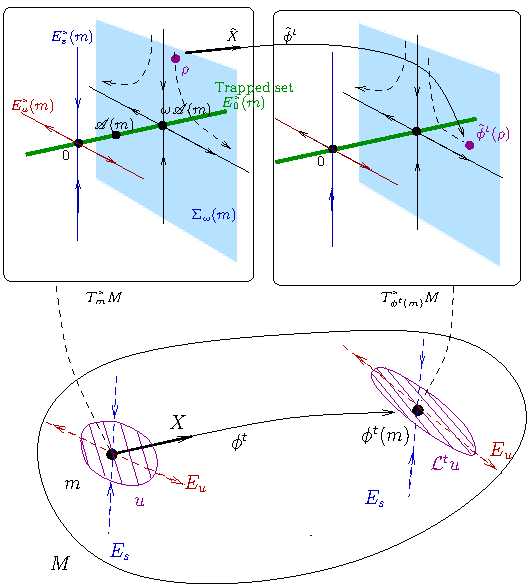
\includegraphics[scale=1.10]{figures/Cotangent-1.pdf} 
\vspace*{-5pt}
\caption{The Anosov flow $\phi^{t}=\exp(tX)$ on $M$ is lifted to a Hamiltonian flow $\tilde{\phi}^{t}=\exp(t\tilde{X})$ in the cotangent bundle $T^{*}M$. The lines on the base~(in magenta) represent ``internal oscillations'' of a function $u$ at point $m\in M$. These oscillations correspond to a cotangent vector $\rho\in T_{m}^{*}M$. Transported by the flow $\phi^{t}$, these oscillations become parallel to $E_{u}$, i.e. the direction of $\tilde{\phi}^{t}(\rho)$ converges to $E_{u}^{*}\subset T^{*}M$ and $\tilde{\phi}^{t}(\rho)$ remains in the frequency level $\Sigma_{\omega}:=\boldsymbol{\omega}^{-1}(\omega)$ (in blue). The trapped set $E_{0}^{*}$ (in green) of the lifted flow $\tilde{\phi^{t}}$ is the H\"older continuous rank one vector bundle $E_{0}^{*}=\bbR\scrA$ where $\scrA$ is the Anosov one form.}
\label{fig:The-Anosov-flow-on_T*M}
\vspace*{-10pt}
\end{figure}


\subsection{Escape function \texorpdfstring{$W$}{W}}
\label{subsec:Escape-function-}
In Lemma~\ref{lem:semi_group}, in order to show that the transfer operators $\clL^{t}$ acts on the generalized Sobolev space $\clH _{W}(M)$ as a strongly continuous (semi-)group, we required two properties of the weight function $W$, namely the temperate property~\eqref{eq:temperate_property-W-2} and the boundedness property~\eqref{eq:bound_C} with respect to the lifted flow $\tilde{\phi}^{t}$.

In the next section, we will show that the generator $A$ has discrete Ruelle spectrum. For this we need to reinforce the properties of the weight function $W$ by the slowly varying and temperate property in Definition~\ref{def:temperate_W} and the decay property in Definition~\ref{def:decay_W} below. In Section~\ref{subsec:Escape-function} we also provide an example of a weight function $W$ on $T^{*}M$ satisfying such conditions. Another example of weight function similar to the weight function used in~\cite{fred-roy-sjostrand-07,fred_flow_09} is given in Appendix~\ref{sec:Second-example-of}. (However this latter example does not satisfies~\eqref{eq:estim2} that provides the group property of $\clL^{t}$).

\subsubsection{Requirements for an escape function \texorpdfstring{$W$}{W} on \texorpdfstring{$T^{*}M$}{T*M}}

For a point $m\in M$, recall the decomposition of a cotangent vector $\rho=\rho_{u}+\rho_{s}+\rho_{0}\in T_{m}^{*}M$, in Eq.\eqref{eq:decomp_Xi}. For $0\leq\gamma<1$, we define the continuous function $h_{\gamma}\in C(T^{*}M;\bbR^{+})$ by
\begin{equation}\label{eq:h_gamma}
h_{\gamma}^{\perp}\left(\rho\right):=\left\langle \left\Vert \rho_{u}+\rho_{s}\right\Vert _{g_{\rho}}\right\rangle ^{-\gamma}
\end{equation}
where the vertical vector $\rho_{u}+\rho_{s}\in T_{m}^{*}M$ is naturally identified with a vector in the tangent space $T_{\rho}(T^{*}M)$ of $T^{*}M$ at $\rho\in T^{*}M$ in order to get its norm. Remark that if $\gamma>0$ then $h_{\gamma}^{\perp}(\rho)$ decays as $\rho$ gets far from the trapped set $E_{0}^{*}$. But for some arguments we will sometimes need $\gamma=0$. See Section~\ref{subsec:Remarks-about-the} where we comment on the use of function $h_{\gamma}^{\perp}$ and parameter $h_{0}$.

\begin{cBoxA}{}
\begin{defi}[slowly varying and $h_{\gamma}^{\perp}$-temperate property for a
weight function $W$]\label{def:temperate_W}
A (family of) continuous function $W\in C(T^{*}M;\bbR^{+})$ that depends on $h_{0}>0$, is said to be slowly varying and $h_{\gamma}^{\perp}$ -temperate, if there exists $0<\mu<1$, $C_{W}>0$ and $N_{W}\geq0$ independent of $h_{0}$ such that
\begin{equation}\label{eq:slow_variation_W}
\frac{W\left(\rho'\right)}{W\left(\rho\right)}\leq1+C_{W}h_{0}^{\mu}\left\langle h_{\gamma}^{\perp}\left(\rho\right)\,\dist_{g}\left(\rho',\rho\right)\right\rangle ^{N_{W}}\qquad\text{for all }\rho,\rho'\in T^{*}M.
\end{equation}
\end{defi}
\end{cBoxA}

\begin{rema}
Definition~\eqref{eq:slow_variation_W} expresses two properties. First that for small $h_{0}$ and for any two points $\rho,\rho'$ such that $\dist_{g}(\rho',\rho)\leq h_{\gamma}^{\perp}(\rho)^{-1}$ where $h_{\gamma}^{\perp}(\rho)^{-1}$ can be large, then $W$ has ratio close to 1, i.e. slow variations. Second that, at larger distances, $W$ has temperate variations which grow at most polynomial rate in $(h_{\gamma}^{\perp}(\rho)\dist_{g}(\rho',\rho))$.
\end{rema}


\begin{rema}
Eq.\eqref{eq:slow_variation_W} can be written as
\begin{equation}\label{eq:slow_variation_W-1}
\left|W\left(\rho'\right)-W\left(\rho\right)\right|\leq W\left(\rho\right)C_{W}h_{0}^{\mu}\left\langle h_{\gamma}^{\perp}\left(\rho\right)\dist_{g}\left(\rho',\rho\right)\right\rangle ^{N_{W}},
\end{equation}
and implies $\forall\rho,\rho'\in T^{*}M$,
\begin{equation}\label{eq:temperate_property}
\frac{W\left(\rho'\right)}{W\left(\rho\right)}\leq C'_{W}\left\langle h_{0}^{\mu/N_{W}}h_{\gamma}^{\perp}\left(\rho\right)\dist_{g}\left(\rho',\rho\right)\right\rangle ^{N_{W}}\leq C'_{W}\left\langle h_{0}^{\mu/N_{W}}\dist_{g}\left(\rho',\rho\right)\right\rangle ^{N_{W}},
\end{equation}
with $C'_{W}>0$ independent of $h_{0}$ and $N_{W}$. In particular Eq.~\eqref{eq:slow_variation_W-1} shows that according to Definition~\ref{def:Let--be}, the function $W$ is $h,N_0,h_0$-slowly varying with function $h=C_{W}h_{0}^{\mu}W$.\linebreak We will use this later in the proof of Lemma~\ref{lem:For-the-weight}. Also, Eq.~\eqref{eq:temperate_property} shows that according to Definition~\ref{def:temperate_W-1}, the function $W$ is temperate so the results of Section~\ref{sec:Semiclassical-analysis-with} apply.\linebreak We will use~\eqref{eq:temperate_property} later in the proof of Lemma~\ref{lem:For-the-weight} and of Theorem~\ref{thm:decay_outside_trapped_set}.
\end{rema}



\begin{cBoxA}{}
\begin{defi}[Decay property for a weight function $W$]\label{def:decay_W}
A continuous function $W\in C(T^{*}M;\bbR^{+})$ has time decay property with rate $\Lambda>0$ with respect to the flow $(\tilde{\phi}^{t})_{t\,\geq\,0}$, if there exists a constant $C>1$ such that, for any $t\geq0$, one can take $C_{W,t}>0$ so that
\begin{equation}\label{eq:decay_property}
\frac{W\left(\tilde{\phi}^{t}\left(\rho\right)\right)}{W\left(\rho\right)}\leq
\begin{cases}
C\\
Ce^{-\Lambda t} & \text{ if }\left\Vert \rho_{u}+\rho_{s}\right\Vert _{g\left(\rho\right)}>C_{W,t}\quad\text{for any \ensuremath{\rho\in T^{*}M}.}
\end{cases}
\end{equation}
Moreover $W$ has a decay controlled from below with rate $\Lambda'\geq0$ if there exists a constant $C>1$ such that
\begin{equation}\label{eq:decay_property-1}
\frac{W\left(\tilde{\phi}^{t}\left(\rho\right)\right)}{W\left(\rho\right)}\geq\frac{1}{C}e^{-\Lambda't} \quad\text{for any \ensuremath{\rho\in T^{*}M}\text{ and }\ensuremath{t\ge0}}.
\end{equation}
\end{defi}
\end{cBoxA}

\begin{rema}
The general bound $W(\tilde{\phi}^{t}(\rho)/W(\rho)\leq C$ given by the first line of~\eqref{eq:decay_property} together with the temperate property has been used in the proof of Lemma~\ref{lem:semi_group} in order to show that the transfer operator $\clL^{t}:\clH _{W}(M)\rightarrow\clH _{W}(M)$ is bounded and forms a strongly continuous semi-group. The bound from below~\eqref{eq:decay_property-1} has been used in Lemma~\ref{lem:semi_group} to show that $\clL^{t}:\clH _{W}(M)\rightarrow\clH _{W}(M),t\in\bbR$ forms a strongly continuous group.

The more precise bound given in the second line of~\eqref{eq:decay_property} shows that we have time decay outside the trapped set $E_{0}^{*}$. It will be used in the proof of Lemma~\ref{lem:bounded_resolvent_of_A'} to show that the transfer operator $\clL^{t}$ has small norm outside the trapped set and to deduce discrete spectrum of its generator. The fact that the constant $C_{w,t}$ depends on time $t$ in~\eqref{eq:decay_property} is due to the fact that a trajectory close to the stable manifold of the trapped set $E_{0}^{*}$ can spend a long time close to the trapped set where there is no decay. During that time, a wave packet spreads exponentially.
\end{rema}


\subsubsection{Example of weight function \texorpdfstring{$W$}{W}}\label{subsec:Escape-function}

We provide here an example of escape function $W$ and we prove that $W$ satisfies the properties of being temperate, slowly varying and decay property given above in Definitions~\ref{def:temperate_W} and~\ref{def:decay_W}.

Recall from~\eqref{eq:def_beta_*} that the H\"older exponents satisfy $\min(\beta_{u},\beta_{s})\leq\beta_{0}$ and recall that the parameters $\alpha^{\perp}$,$\alpha^{\parallel}$ that enter in the definition of the metric $g$ in~\eqref{eq:def_delta}.

Before giving the definition of $W$ we need, for technical reasons\footnote{The use of this modified metric $\tilde{g}$ instead of $g$ will permit to provide a simpler proof, compared to a previous proof given in the \href{https://arxiv.org/pdf/1706.09307v2.pdf\#page=52}{version v2} of this paper on ArXiv, that uses the metric $g$ itself.}, to use a slightly different norm on $TT_{m}^{*}M$ for $m\in M$, defined as follows. Let $g_{M}$ be a global smooth metric on $M$. Let $\tilde{g}_{M}$ be the metric on $T_{m}M,m\in M$, that equals $g_{M}$ on $E_{\sigma}$ for $\sigma=u,s,0$ and such that the sum $E_{u}\oplus E_{s}\oplus E_{0}$ is orthogonal. As a consequence $g_{M}$ is H\"older continuous on $M$ and the dual sum $E_{u}^{*}\oplus E_{s}^{*}\oplus E_{0}^{*}$ is also orthogonal for the induced metric on $T_{m}^{*}M$, $m\in M$, that we still denote by $\tilde{g}_{M}$. Now we define the metric $\tilde{g}$ on $TT_{m}^{*}M,m\in M,$ as follows. For $\tilde{v}=(\tilde{v}_{\xi},\tilde{v}_{\omega})\in T_{\rho}T_{m}^{*}M$, with $m\in M,\rho\in T_{m}^{*}M$, $\tilde{v}_{\xi}\in E_{u}^{*}\oplus E_{s}^{*}$, $\tilde{v}_{\omega}\in E_{0}^{*}$, we set
\begin{equation}\label{eq:norm_g-1}
\left\Vert \tilde{v}\right\Vert _{\tilde{g}\left(\rho\right)}^{2}=\left(\left\langle \left\Vert \rho\right\Vert _{\tilde{g}_{M}}\right\rangle ^{-\alpha^{\perp}}\left\Vert \tilde{v}_{\xi}\right\Vert _{\tilde{g}_{M}}\right)^{2}+\left(\left\langle \left\Vert \rho\right\Vert _{\tilde{g}_{M}}\right\rangle ^{-\alpha^{\parallel}}\left\Vert \tilde{v}_{\omega}\right\Vert _{\tilde{g}_{M}}\right)^{2}.
\end{equation}
Let $0<\gamma<1$. We define the continuous function $\tilde{h}_{\gamma}^{\perp}:T^{*}M\rightarrow\bbR^{+}$ as follows. For $\rho=\rho_{u}+\rho_{s}+\rho_{0}\in T^{*}M$, we set
\begin{equation}\label{eq:h_tilde-1}
\tilde{h}_{\gamma}^{\perp}\left(\rho\right)=\left\langle \left\Vert \rho_{u}+\rho_{s}\right\Vert _{\tilde{g}\left(\rho\right)}\right\rangle ^{-\gamma}.
\end{equation}
So notice that the norms $g_{M}$ and $\tilde{g}_{M}$ are equivalent, that the norm of a vertical vector given by $\tilde{g}$ in~\eqref{eq:norm_g-1} is equivalent to the norm given by the metric $g$ defined in~\eqref{eq:metric_g_in_coordinates}, and finally that the function $\tilde{h}_{\gamma}^{\perp}$ defined in~\eqref{eq:h_tilde-1} looks like the function $h_{\gamma}^{\perp}$ defined in~\eqref{eq:h_gamma}, except that we use now the metric $\tilde{g}$ instead of $g$.

\begin{cBoxA}{}
\begin{defi}[Example of a weight function $W$ with good properties]\label{def:def_W1}
Assume that $\alpha^{\perp}$ and $\alpha^{\parallel}$ satisfy
\begin{equation}\label{eq:ineq1}
\frac{1}{1+\beta_{0}}\leq\alpha^{\perp}<1,\quad0\leq\alpha^{\parallel}\leq\alpha^{\perp}.
\end{equation}
For $\gamma\in[0,1[$ such that
\begin{equation}\label{eq:gamma_interval}
1-\frac{\alpha^{\perp}\min\left(\beta_{u},\beta_{s}\right)}{1-\alpha^{\perp}}\leq\gamma<1,
\end{equation}
and $R_{u}>0$, $R_{s}>0$, $h_{0}>0$, we define the \emph{escape function} $W:T^{*}M\rightarrow\bbR^{+}$ by
\begin{equation}\label{eq:def_W1}
W\left(\rho\right):=\frac{\left\langle h_{0}\tilde{h}_{\gamma}^{\perp}\left(\rho\right)\left\Vert \rho_{s}\right\Vert _{\tilde{g}\left(\rho\right)}\right\rangle ^{R_{s}}}{\left\langle h_{0}\tilde{h}_{\gamma}^{\perp}\left(\rho\right)\left\Vert \rho_{u}\right\Vert _{\tilde{g}\left(\rho\right)}\right\rangle ^{R_{u}}}.
\end{equation}
\end{defi}
\end{cBoxA}

\begin{rema}
In the expression~\eqref{eq:def_W1} for $W$, we can write in a more concise way $h_{0}h_{\gamma}^{\perp}(\rho)\Vert \rho_{s}\Vert _{\tilde{g}(\rho)}=\Vert \rho_{s}\Vert _{\tilde{g}_{\gamma,h_{0}}(\rho)}$ using the metric $\tilde{g}_{\gamma,h_{0}}:=(h_{0}h_{\gamma}^{\perp})^{2}\tilde{g}$ that is conformal to $\tilde{g}$.
\end{rema}


\begin{rema}
The meaning of Definition~\ref{def:def_W1} will be discussed in Section~\ref{rem:Due-to-the}. The way to chose optimally the different parameters that enter in the construction of $W$ for the analysis of Anosov flow will be discussed in Section~\ref{subsec:Optimal-values-of}. We first give the following theorem that shows that $W$ has the required properties.
\end{rema}

\begin{cBoxB}{}
\begin{theo}\label{thm:W}
The weight function $W$ in~\eqref{eq:def_W1} has the following properties
\begin{enumerate}
\item \label{enu:-satisfies--temperate-1}
$W$ satisfies the slowly varying and $h_{\gamma}^{\perp}$ -temperate property~\eqref{eq:slow_variation_W}.
\item \label{enu:-satisfies-decay-1}
$W$ satisfies the decay property~\eqref{eq:decay_property} with rate
\begin{equation}\label{eq:def_Lambda}
\Lambda=\lambda_{\min}\left(1-\gamma\right)\left(1-\alpha^{\perp}\right)\min\left(R_{s},R_{u}\right).
\end{equation}
\item \label{enu:-satisfies-decay-below}
$W$ satisfies the decay property controlled from below~\eqref{eq:decay_property} with rate
\begin{equation}\label{eq:lAMBDA_P}
\Lambda'=\lambda_{\max}\left(1-\gamma\right)\left(1-\alpha^{\perp}\right)\left(R_{s}+R_{u}\right).
\end{equation}
\item \label{enu:Its-order-is-1}
Its order, defined in~\eqref{eq:def_order-2}, is
\begin{equation}\label{eq:order_of_W1}
r\left(\left[\rho\right]\right)=
\begin{cases}
0, & \text{along \ensuremath{E_{0}^{*}}; }\\
-\left(1-\gamma\right)\left(1-\alpha^{\perp}\right)R_{u} & \text{along \ensuremath{E_{u}^{*}};}\\
\left(1-\gamma\right)\left(1-\alpha^{\perp}\right)R_{s} & \text{along \ensuremath{E_{s}^{*}};}\\
\left(1-\gamma\right)\left(1-\alpha^{\perp}\right)\left(R_{s}-R_{u}\right) & \text{along all other directions.}
\end{cases}
\end{equation}
\end{enumerate}
\end{theo}
\end{cBoxB}

The proof of Theorem~\ref{thm:W} is given in Section~\ref{subsec:Proof-of-Thm}. From the weight function $W$ in~\eqref{eq:def_W1}, we can define the Sobolev space $\clH _{W}(M)$ from Definition~\ref{def:Anisotropic_Sob_space}. We will use this (anisotropic) Sobolev space in the next section.


\begin{rema}
One can consider other weight functions that satisfy the required properties. For example in Appendix~\ref{sec:Second-example-of} one gives a second example of weight function $W_{2}$ that has been introduced in~\cite{fred-roy-sjostrand-07,fred_flow_09} and used many times since in the literature. We also compare the (dis)advantages of these two weight functions in Appendix~\ref{sec:Second-example-of}.
\end{rema}


\subsubsection{Remarks on the weight function \texorpdfstring{$W$}{W}}\label{rem:Due-to-the}

We discuss here the construction of $W$ in~\eqref{eq:def_W1} and the meaning of the inequalities~\eqref{eq:ineq1} and~\eqref{eq:gamma_interval}. First observe one main feature of~\eqref{eq:def_W1} : $W(\rho)$ increases with respect to $\Vert \rho_{s}\Vert _{g_{M}}$ and decreases with respect to $\Vert \rho_{u}\Vert _{g_{M}}$. Due to~\eqref{hyperbolicity_xi} this will give the decay property~\eqref{eq:decay_property} of $W$. However, instead of using $\Vert \rho_{s}\Vert _{g_{M}}$ directly we use $h_{\gamma}^{\perp}(\rho)\Vert \rho_{s}\Vert _{g}$ that measures $\rho_{s}$ at the scale of wave packets or greater and this will give the slow varying and temperate property of $W$. In Section~\ref{subsec:Heuristic-explanation-of} and in Figure~\ref{fig:fractal_bound} we have explained heuristically that the choice of parameter $\alpha^{\perp}\geq\frac{1}{1+\beta_{0}}$ for the metric $g$ is necessary in order that unit box of the metric $g$ (i.e. the size or uncertainty of a wave-packet) is greater than the H\"older fluctuations of the trapped set $E_{0}^{*}$ and therefore absorb or hide them. This explains~\eqref{eq:ineq1}. We should have similar properties for the directions~$E_{s}^{*}$ and $E_{u}^{*}$ that are also H\"older continue and a natural construction would have been to define a metric $g$ with exponents $\alpha_{s}^{\perp},\alpha_{u}^{\perp}$ that satisfy $\alpha_{u}^{\perp}\geq\frac{1}{1+\beta_{u}},\alpha_{s}^{\perp}\geq\frac{1}{1+\beta_{s}}$. We are not been able to do this because our specific construction of the metric $g$ needs the same exponent $\alpha^{\perp}$ in every transverse directions. In order to overcome this technical problem we have introduced instead the scaling (or conformal) factor $h_{\gamma}^{\perp}(\rho)$ in the construction of $W$, \eqref{eq:def_W1}, with some exponent $\gamma$ that plays a role similar to $\alpha_{u}^{\perp},\alpha_{s}^{\perp}$. However this scaling factor in the fibers of $T^{*}M$ is not equivalent (it is weaker in fact) to choosing a different metric on $T^{*}M$ compatible with the symplectic form.

Let us explain now the range of $\gamma$ in~\eqref{eq:gamma_interval}. At a point $\rho\in T^{*}M$ we consider a unit box of the metric $g$ that has horizontal transverse size $\delta m\asymp\delta^{\perp}(\rho)\asymp|\rho|^{-\alpha^{\perp}}$. The H\"older exponents $\beta_{s}$ implies that fluctuations of $E_{s}^{*}$ are smaller than $|\rho_{s}|(\delta m)^{\beta_{s}}\asymp|\rho_{s}||\rho|^{-\alpha^{\perp}\beta_{s}}$. Near this direction we have $h_{\gamma}^{\perp}(\rho)^{-1}\asymp(|\rho|^{-\alpha^{\perp}}|\rho_{s}|)^{\gamma}\asymp|\rho_{s}|^{\gamma}|\rho|^{-\alpha^{\perp}\gamma}$. The unit boxes for the re-scaled metric $(h_{\gamma}^{\perp})^{2}g$ have size $\Delta\rho\asymp(h_{\gamma}^{\perp}(\rho)\delta^{\perp}(\rho))^{-1}\asymp|\rho_{s}|^{\gamma}|\rho|^{\alpha^{\perp}(1-\gamma)}$. In order that these unit boxes absorb the fluctuations of $E_{s}^{*}$, we require the condition
\begin{align*}
\Delta\rho \geq\left|\rho_{s}\right|\left(\delta m\right)^{\beta_{*}}\;\; &\Longleftrightarrow\;\left|\rho_{s}\right|^{\gamma}\left|\rho\right|^{\alpha^{\perp}\left(1-\gamma\right)}\,\geq\left|\rho_{s}\right|\left|\rho\right|^{-\alpha^{\perp}\beta_{s}}\\
&\Longleftrightarrow\;\left|\rho\right|^{\alpha^{\perp}\left(1-\gamma\right)+\alpha^{\perp}\beta_{s}}\geq\left|\rho_{s}\right|^{1-\gamma}.
\end{align*}
Since $|\rho_{s}|\leq|\rho|$, this follows if we assume
\[
\alpha^{\perp}\left(1-\gamma\right)+\alpha^{\perp}\beta_{s}\geq1-\gamma\quad\Longleftrightarrow\quad\gamma\geq1-\frac{\alpha^{\perp}\beta_{s}}{1-\alpha^{\perp}}.
\]
With the same consideration for $E_{u}^{*}$, we are led to the condition on $\gamma$ that appears in~\eqref{eq:gamma_interval}. See Figure~\ref{fig:zones-W}.

\begin{figure}[!htbp]
\centering
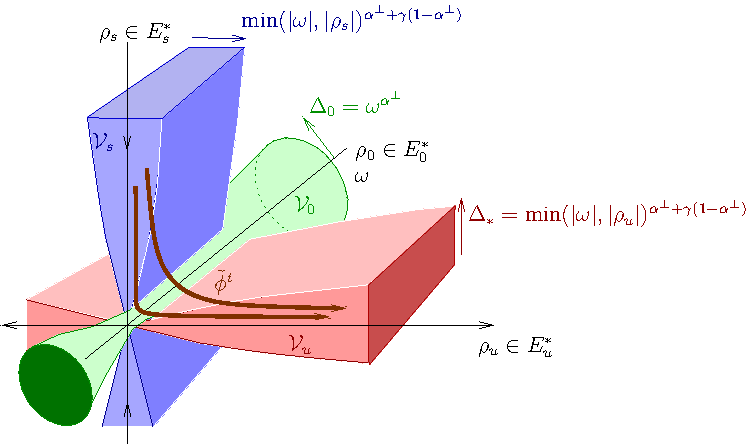
\includegraphics[scale=1]{figures/zones_W2-1.pdf} 
\caption{Representation of domains associated to the weight function $W$ defined in~\eqref{eq:def_W1}: $\clV_{s}$ is the (blue) the \textquotedblleft parabolic\textquotedblright{} neighborhood of $E_{s}^{*}$ given by
\[
\clV_{s}:=\left\{ \rho;\,\left\langle h_{\gamma}^{\perp}\left(\rho\right)\left\Vert \rho_{u}\right\Vert _{g_{\rho}}\right\rangle \asymp1\right\} =\left\{ \rho;\,\left|\rho_{u}\right|\apprle\min\left(\left|\omega\right|,\left|\rho_{s}\right|\right)^{\alpha^{\perp}+\gamma\left(1-\alpha^{\perp}\right)}\right\},
\]
similarly for $\clV_{u}$, and 
\[
\clV_{0}:=\clV_{u}\cap\clV_{s}=\left\{ \rho;\,\left|\rho_{u}+\rho_{s}\right|\apprle\omega^{\alpha^{\perp}}\right\}.
\]
Outside this domain $\clV_{0}$ (in green), the weight function $W$ decays along the flow~$\tilde{\phi}^{t}$.}
\label{fig:zones-W}
\end{figure}


\subsubsection{Remarks about optimal values of parameters for the weight function \texorpdfstring{$W$}{W}}\label{subsec:Optimal-values-of}

In this section we comment the optimal choice of weight function $W$ in order to get the theorems of this paper. Recall that, in Section~\ref{subsec:A-metric}, the metric $g$ on $T^{*}M$ is defined depending on the parameters $\alpha^{\perp},\alpha^{\parallel}$ which satisfy $0\leq\alpha^{\parallel}<\alpha^{\perp}<1,\frac{1}{2}\linebreak\leq\alpha^{\perp}<1$ from~\eqref{eq:conditions}.

The weight function $W$ depends on additional parameters $h_{0}>0$, $R_{u},R_{s}>0,\gamma\geq0$ and Theorem~\ref{thm:W} give their admissible range of values. Also the admissible range of $\alpha^{\perp}$ is restricted to $\frac{1}{1+\beta_{0}}\leq\alpha^{\perp}<1$. (See Lemma~\ref{thm:W} and Remark~\ref{rem:Due-to-the}.) According to these constraints we will consider optimal values of these parameters depending on the purpose.

\paragraph{Choice 1 of $W$ to estimate the density of eigenvalues (Weyl law):}

In order to prove Theorem~\ref{thm:Weyl law} about the Weyl law for the density of eigenvalues, we will take, after Lemma~\ref{prop:discrete_spectrum}, the minimal allowed value for $\alpha^{\perp},\alpha^{\parallel}$ and $\gamma$ that are
\[
\alpha^{\perp}=\frac{1}{1+\beta_{0}},\quad\alpha^{\parallel}=0,\quad\gamma\eq{\ref{eq:gamma_interval}}1-\frac{\beta_{*}}{\beta_{0}}\quad\text{with setting }\beta_{*}=\min\left(\beta_{u},\beta_{s}\right)\le\beta_{0}.
\]

\pagebreak

\noindent that satisfy the assumptions~\eqref{eq:ineq1} and~\eqref{eq:gamma_interval}. The choice of these optimal values were explained in Section~\ref{subsec:Heuristic-explanation-of}. See also Figure~\ref{fig:zones-W} where they give that the transverse size for the (green) region $\clV_{0}$ is
\[
\Delta_{0}^{\left(1\right)}=\omega^{\frac{1}{1+\beta_{0}}}.
\]
However, for this choice, the transverse size of the region $\clV_{u}$ on Figure~\ref{fig:zones-W} is
\begin{equation}\label{eq:Delta_1*}
\Delta_{*}^{\left(1\right)}:=\left|\rho_{u}\right|^{\alpha^{\perp}+\gamma\left(1-\alpha^{\perp}\right)}=\left|\rho_{u}\right|^{1-\frac{\beta_{*}}{1+\beta_{0}}}.
\end{equation}
This choice is not optimal to study the concentration of the wave front set and one can improve with Choice 2 below.

\paragraph{Choice 2 of $W$ to estimate the concentration of the wave front set:}\ \\*[-1.2em]

\noindent In Corollary~\ref{cor:Let-us-choose} that concerns the width exponent of the parabolic wave front set of Ruelle resonances, we choose the following values
\begin{equation}\label{eq:choice_2}
\alpha^{\perp}=\frac{1}{1+\beta_{*}},\quad\alpha^{\parallel}=0,\quad\gamma\eq{\eqref{eq:gamma_interval}}0,\quad\text{with setting }\beta_{*}=\min\left(\beta_{u},\beta_{s}\right)\le\beta_{0}.
\end{equation}
that satisfy the assumptions~\eqref{eq:ineq1} and~\eqref{eq:gamma_interval}. The reason for this choice is that the transverse size $\Delta_{*}^{(2)}$ of the region $\clV_{u}$ on Figure~\ref{fig:zones-W} is
\begin{equation}\label{eq:size_Delta_2*}
\Delta_{*}^{\left(2\right)}:=\left|\rho_{u}\right|^{\alpha^{\perp}+\gamma\left(1-\alpha^{\perp}\right)}=\left|\rho_{u}\right|^{\frac{1}{1+\beta_{*}}}
\end{equation}
and smaller than $\Delta_{*}^{(1)}$ in~\eqref{eq:Delta_1*}, (except for the case $\beta_{*}=\beta_{0}$)
\[
\Delta_{*}^{\left(2\right)}\leq\Delta_{*}^{\left(1\right)}
\]
because
\begin{multline*}
\frac{1}{1+\beta_{*}}<1-\frac{\beta_{*}}{1+\beta_{0}}\\\Longleftrightarrow
1+\beta_{0}<(1+\beta_{*})(1+\beta_{0}-\beta_{*})=1+\beta_{0}+\beta_{*}(\beta_{0}-\beta_{*}).
\end{multline*}
However this choice gives the transverse size $\Delta_{0}^{(2)}$ of the green region $\clV_{0}$ that is greater than $\Delta_{0}^{(1)}$:
\[
\Delta_{0}^{\left(2\right)}=\omega^{\frac{1}{1+\beta_{*}}}\geq\Delta_{0}^{\left(1\right)}.
\]
Therefore this choice is not adequate to deduce Theorem~\ref{thm:Weyl law} about the Weyl law.

\subsubsection{Remarks about the use of parameter \texorpdfstring{$h_{0}$}{h0} and function \texorpdfstring{$h_{\gamma}^{\perp}\left(\rho\right)$}{h gamma perp(rho)}}\label{subsec:Remarks-about-the}

The definition~\eqref{eq:def_W1} for the function $W$ makes use of the product $h_{0}\tilde{h}_{\gamma}^{\perp}(\rho)$ with a parameter $h_{0}$ and a function $\tilde{h}_{\gamma}^{\perp}(\rho)=\langle \Vert \rho_{u}+\rho_{s}\Vert _{\tilde{g}(\rho)}\rangle ^{-\gamma}$ that depends on the parameter $\gamma\geq0$. We have already comment about the meaning and utility of the parameter $\gamma$, in the previous Section~\ref{subsec:Optimal-values-of}.

One effect of the product $h_{0}\tilde{h}_{\gamma}^{\perp}(\rho)\ll1$ when it is small is to assure that the ratio of variations of the function $W$ is close to one on a large scale $(h_{0}h_{\gamma}^{\perp})^{-1}\gg1$ and is used as follows in our micro-local analysis: if we consider a wave packet (with initial size of order $1$ measured by the metric $g$) that evolves and get size $e^{\lambda t}$ after a given long time $t$ where $\lambda$ is the Lyapunov exponent, then the wave packet still feels the function $W$ as almost constant provided $e^{\lambda t}\ll(h_{0}h_{\gamma}^{\perp})^{-1}$. We use crucially this argument at the end of proof of Lemma~\ref{lem:For-the-weight} and Theorem~\ref{thm:decay_outside_trapped_set}, where we take first $t$ large to get effect of hyperbolicity and after we take $h_{0}$ small. Notice in Theorem~\ref{thm:decay_outside_trapped_set} we consider the outside of the trapped set, where $\Vert \rho_{u}+\rho_{s}\Vert _{\tilde{g}(\rho)}$ is large, so we may have used $h_{\gamma}^{\perp}(\rho)\ll1$ for this purpose but only if we assume $\gamma>0$. However there are some cases where need to take $\gamma=0$, see~\eqref{eq:choice_2}, giving $h_{\gamma}^{\perp}(\rho)=1$ that is not small. So for simplicity we always use $h_{0}$ as the small parameter.

\subsection{\label{subsec:Discrete-Spectrum-and}
Discrete Spectrum and Weyl law upper bound}

In this section, we prove Theorem~\ref{thm:grey-band} about strong continuity of the transfer operators $\clL^{t}$ and Theorem~\ref{thm:Discrete_spectrum} and~\ref{thm:Weyl law} about discrete spectrum and an analogue of the Weyl law. We henceforth assume that the weight function $W$ is chosen from the family~\eqref{eq:def_W1} and we consider the anisotropic Sobolev space $\clH _{W}=\clH _{W}\left(M\right)$ defined in~\eqref{eq:def_H_W}. Recall that the definition of $W$ depends on the parameters $R_{u}$, $R_{s}$, $\gamma$ and $h_{0}$ besides the parameters $\alpha^{\perp},\alpha^{\parallel}$ used in the definition of the metric $g$ on $T^{*}M$. From~\eqref{eq:order_of_W1}, the parameters $R_{u}$ and $R_{s}$ determine the order of the function $W$ at infinity, while the parameters $\gamma$ and $h_{0}$ are related to the variation of $W$ in smaller scales.

\subsubsection{Strong continuity}

From Lemma~\ref{lem:semi_group}, it follows immediately that $\Vert \clL^{t}\Vert _{\clH _{W}}\leq Ce^{tC_{X,V,W}}$ for $t\ge0$ with a constant $C_{X,V,W}$ depending on $X,V$ and $W$. The next lemma shows that, if we choose the parameter $h_{0}$ (that enters in $W$ in~\eqref{eq:h_gamma}) depending on the choice of $R_{u}$, $R_{s}$ and $\gamma$, then we may assume that the constant $C_{X,V,W}$ is uniform i.e. does not depend on $W$. Let us recall the constants $C_{X,V}$ and $C'_{X,V}$ defined in~\eqref{eq:C_XV} and~\eqref{eq:C_XV-1}.

\begin{cBoxB}{}
\begin{lemm}[Strong continuity of transfer operators $\clL^{t}$ (version2)]\label{lem:For-the-weight}
For any $\epsilon>0$, there exists $C>0$, for any parameters $R_{u},R_{s}>0$, we can choose $h_{0}>0$ in~\eqref{eq:h_gamma} small enough so that, for any $t\geq0$, we have
\begin{align}
\left\Vert \clL^{t}\right\Vert _{\clH _{W}} &\leq Ce^{t\left(C_{X,V}+\epsilon\right)},\label{eq:bound_C_X,V}
\\
\intertext{and}
\left\Vert \clL^{-t}\right\Vert _{\clH _{W}} &\leq Ce^{-t\left(C'_{X,V}-\Lambda'-\epsilon\right)},\label{eq:bound_C_X,V-1}
\end{align}
where $\Lambda'$ is given in~\eqref{eq:lAMBDA_P}.
\end{lemm}
\end{cBoxB}

\begin{rema}
From Hille--Yosida--Feller--Miyadera--Phillips's Theorem~\cite[p.~77]{engel_1999}, Eq.~\eqref{eq:bound_C_X,V} implies estimates on the norm of the resolvent $(z-A)^{-1}$ of the generator $A=-X+V$ for $\Ree(z)>C_{X,V}$.
\end{rema}

\begin{proof}
We prove~\eqref{eq:bound_C_X,V}. We have that
\[
\left\Vert \clL^{t}\right\Vert _{\clH _{W}}\underset{\eqref{eq:compare_norms}}{=}\left\Vert \clM_{W}\text{\ensuremath{\clT}\ensuremath{\clL^{t}}\ensuremath{\clT^{\dagger}}}\clM_{W^{-1}}\right\Vert _{L^{2}}.
\]
We write
\begin{equation}\label{eq:decomp}
\clM_{W}\text{\ensuremath{\clT}\ensuremath{\clL^{t}}\ensuremath{\clT^{\dagger}}}\clM_{W^{-1}}=\left(\ensuremath{\clT}\ensuremath{\clL^{t}}\ensuremath{\clT^{\dagger}}\right)\clM_{\left(W\circ\tilde{\phi}^{t}\right)/W}+R
\end{equation}
with remainder operator
\begin{equation}\label{eq:def_R-1}
\begin{split}
R & {:=}\clM_{W}\text{\ensuremath{\clT}\ensuremath{\clL^{t}}\ensuremath{\clT^{\dagger}}}\clM_{W^{-1}}-\text{\ensuremath{\clT}\ensuremath{\clL^{t}}\ensuremath{\clT^{\dagger}}}\clM_{\left(W\circ\tilde{\phi}^{t}\right)/W}
\\
& \;=\left(\clM_{W}\text{\ensuremath{\clT}\ensuremath{\clL^{t}}\ensuremath{\clT^{\dagger}}}-\text{\ensuremath{\clT}\ensuremath{\clL^{t}}\ensuremath{\clT^{\dagger}}}\clM_{W\circ\tilde{\phi}^{t}}\right)\clM_{W^{-1}}.
\end{split}
\end{equation}
We apply Theorem~\ref{thm:Microlocality-of-the_TO} and Theorem~\ref{thm:W} that gives~\eqref{eq:slow_variation_W-1} and we get
\begin{equation}
\begin{split} 
\left|\langle\delta_{\rho',j'}|R\delta_{\rho,j}\rangle\right|&\underset{\eqref{eq:def_R-1}}{=} \left|\langle\delta_{\rho',j'}|\text{\ensuremath{\clT}\ensuremath{\clL^{t}}\ensuremath{\clT^{\dagger}}}\delta_{\rho,j}\rangle\right|\left|W\left(\rho'\right)-W\left(\tilde{\phi}^{t}\left(\rho\right)\right)\right|W^{-1}\left(\rho\right)\\
&\mkern-15mu\underset{\eqref{eq:microl_estimate},\eqref{eq:slow_variation_W-1}}{\leq} \left(W\left(\rho'\right)C_{W}h_{0}^{\mu}\left\langle h_{\gamma}^{\perp}\left(\tilde{\phi}^{t}\left(\rho\right)\right)\dist_{g}\left(\rho',\tilde{\phi}^{t}\left(\rho\right)\right)\right\rangle ^{N_{W}}\right)\\
\end{split}
\end{equation}
\begin{align}
&\mkern-15mu\left(C_{N,t}\left\langle \dist_{g}\left(\rho',\tilde{\phi}^{t}\left(\rho\right)\right)\right\rangle ^{-N}\right)W^{-1}\left(\rho\right)\\
&\leq  C_{N,t}h_{0}^{\mu}C_{W}\left(\frac{W\left(\rho'\right)}{W\left(\tilde{\phi}^{t}\left(\rho\right)\right)}\right)\left(\frac{W\left(\tilde{\phi}^{t}\left(\rho\right)\right)}{W\left(\rho\right)}\right)\left\langle \dist_{g}\left(\rho',\tilde{\phi}^{t}\left(\rho\right)\right)\right\rangle ^{-N+N_{W}}\nonumber\\
&\mkern-25mu\underset{\eqref{eq:decay_property},\eqref{eq:temperate_property}}{\leq}  C_{N,t}h_{0}^{\mu}C_{W}C'_{W}\left\langle h_{0}^{\mu/N_{W}}h_{\gamma}^{\perp}\left(\tilde{\phi}^{t}\left(\rho\right)\right)\dist_{g}\left(\rho',\tilde{\phi}^{t}\left(\rho\right)\right)\right\rangle ^{N_{W}}\nonumber\\
&\mkern293mu\left\langle \dist_{g}\left(\rho',\tilde{\phi}^{t}\left(\rho\right)\right)\right\rangle ^{-N+N_{W}}
\nonumber\\
&\leq  C_{N,t}h_{0}^{\mu}C_{W}\left\langle \dist_{g}\left(\rho',\tilde{\phi}^{t}\left(\rho\right)\right)\right\rangle ^{-N+2N_{W}}\nonumber.\label{eq:res_int}
\end{align}
Then by Schur Lemma~\ref{lem:Schur-Lemma-.}, we get
\begin{equation}\label{eq:bound_R}
\left\Vert R\right\Vert _{L^{2}}\le C_{W,N_{W},t}h_{0}^{\mu},
\end{equation}
where the constant $C_{W,N_{W},t}$ depends on $t$ and also on the parameters $R_{u}$, $R_{s},N_{W}$ and $\gamma$ but not on $h_{0}$. We also have
\[
\left\Vert \clM_{W\circ\tilde{\phi}^{t}/W}\right\Vert _{L^{2}}\ineq{\ref{eq:decay_property}}C
\]
with $C$ independent of $t$ and $h_{0}$. Let $0<\epsilon'<\epsilon$. From the choice of $C_{X,V}$ in~\eqref{eq:C_XV}, we have
\[
\left\Vert \ensuremath{\clT}\ensuremath{\clL^{t}}\ensuremath{\clT^{\dagger}}\right\Vert _{L^{2}}\eq{\ref{eq:resol_ident_Pi_rho}}\ensuremath{\left\Vert \clL^{t}\right\Vert _{L^{2}}}\underset{\eqref{eq:L*t*Lt}}{\leq}Ce^{\left(C_{X,V}+\epsilon'\right)t}\quad\text{for }t>0
\]
with $C$ independent of $t$. We obtain
\[
\left\Vert \clM_{W}\text{\ensuremath{\clT}\ensuremath{\clL^{t}}\ensuremath{\clT^{\dagger}}}\clM_{W^{-1}}\right\Vert _{L^{2}}\underset{\eqref{eq:decomp},\eqref{eq:bound_R}}{\leqslant}Ce^{(C_{X,V}+\epsilon')t}+C_{W,N_{W},t}h_{0}^{\mu}\le e^{(C_{X,V}+\epsilon)t}
\]
where the last inequality is obtained by taking $t$ large enough and then $h_{0}$ small enough. By iteration, the last inequality implies~\eqref{eq:bound_C_X,V}. To prove~\eqref{eq:bound_C_X,V-1}, we proceed similarly for the negative time $t<0$ and use~\eqref{eq:decay_property-1} in the place of~\eqref{eq:decay_property}.
\end{proof}

For the next Lemma, let $\sigma>0$ that will be chosen large enough later. Define the following characteristic function $\Lambda_{\sigma}:T^{*}M\rightarrow\bbR^{+}$, such that for every $\rho\in T^{*}M$
\begin{equation*}\label{eq:def_Lambda-1}
\begin{split}
\Lambda_{\sigma}\left(\rho\right) & :=
\begin{cases}
1 & \text{ if }\dist_{g}\left(\rho,E_{0}^{*}\right)\leq\sigma\\
0 & \text{ if }\dist_{g}\left(\rho,E_{0}^{*}\right)>\sigma
\end{cases}.
\end{split}
\end{equation*}
Let
\begin{equation}\label{eq:def_op_Lambda}
\Opp \left(1-\Lambda_{\sigma}\right):=\clT^{\dagger}\left(1-\Lambda_{\sigma}\right)\clT\quad:C^{\infty}\left(M\right)\rightarrow C^{\infty}\left(M\right)
\end{equation}
be the corresponding PDO operator, that removes components near the trapped set. The next Theorem shows that the transfer operator decays very fast on the outer part of the trapped set.

\begin{cBoxB}{}
\begin{theo}[Decay outside the trapped set]\label{thm:decay_outside_trapped_set}
For any $\epsilon>0$, there exists $C>0$, for any parameters $R_{u},R_{s}>0$, we can choose $h_{0}>0$ in~\eqref{eq:h_gamma} small enough so that, for any $t\geq0$, we can choose $\sigma_{t}>0$ large enough and we have
\begin{equation}\label{eq:bound_C_X,V-2}
\left\Vert \clL^{t}\Opp \left(1-\Lambda_{\sigma_{t}}\right)\right\Vert _{\clH _{W}}\leq Ce^{t\left(C_{X,V}-\Lambda+\epsilon\right)},
\end{equation}
where $\Lambda$ is given in~\eqref{eq:def_Lambda}.
\end{theo}
\end{cBoxB}

\begin{proof}
We proceed as in Lemma~\ref{lem:For-the-weight}. For simplicity we write $\Lambda_{\sigma}^{c}=1-\Lambda_{\sigma}$. The operator $\ensuremath{\clL^{t}}\textrm{Op}(\Lambda_{\sigma}^{c})$ on $\clH _{W}(M)$ lifted on $L^{2}(T^{*}M;\bbC^{J})$ is
\begin{align*}
\clM_{W}\text{\ensuremath{\clT}\ensuremath{\clL^{t}}\textrm{Op}\ensuremath{\left(\Lambda_{\sigma}^{c}\right)}\ensuremath{\ensuremath{\clT^{\dagger}}}}\clM_{W^{-1}} & =\ensuremath{\clT}\ensuremath{\clL^{t}}\ensuremath{\clT^{\dagger}}\clM_{\Lambda_{\sigma}^{c}\left(W\circ\tilde{\phi}^{t}\right)/W}Q_{1}+R_{2}
\end{align*}
with
\[
Q_{1}=W\clP W^{-1},\quad Q_{2}=W\clM_{\Lambda_{\sigma}^{c}}\clP W^{-1},
\]
\[
R_{2}=RQ_{2},
\]
and $R=(\clM_{W}\text{\ensuremath{\clT}\ensuremath{\clL^{t}}\ensuremath{\clT^{\dagger}}}-\text{\ensuremath{\clT}\ensuremath{\clL^{t}}\ensuremath{\clT^{\dagger}}}\clM_{W\circ\tilde{\phi}^{t}})\clM_{W^{-1}}$ as in~\eqref{eq:def_R-1}. We have
\[
\left\Vert \ensuremath{\clT}\ensuremath{\clL^{t}}\ensuremath{\clT^{\dagger}}\right\Vert _{L^{2}}\eq{\ref{eq:resol_ident_Pi_rho}}\ensuremath{\left\Vert \clL^{t}\right\Vert _{L^{2}}}\underset{\eqref{eq:L*t*Lt}}{\leq}Ce^{\left(C_{X,V}+\epsilon\right)t}\quad\text{for }t>0.
\]
From the decay property~\eqref{eq:decay_property} of the weight function $W$, we have that if $\sigma$ is large enough depending on $t$ and $W$,
\[
\left\Vert \clM_{\Lambda_{\sigma}^{c}\left(W\circ\tilde{\phi}^{t}\right)/W}\right\Vert _{L^{2}}\ineq{\ref{eq:decay_property}}Ce^{-\Lambda t}.
\]
We have
\begin{align*}
\left|\left\langle\delta_{\rho',j'}\,\middle|\,Q_{1}\delta_{\rho,j}\right\rangle\right| & =\frac{W\left(\rho'\right)}{W\left(\rho\right)}\left|\langle\delta_{\rho',j'}\,\middle|\,\clP \delta_{\rho,j}\rangle\right|\\
& \mkern-29mu\underset{\eqref{eq:temperate_property},\eqref{eq:estimate_Bergman_kernel}}{\leq}C_{W}\left\langle h_{0}^{\mu/N_{W}}\dist_{g}\left(\rho',\rho\right)\right\rangle ^{N_{W}}C_{N}\left\langle \dist_{g}\left(\rho',\rho\right)\right\rangle ^{-N}.
\end{align*}
with $C_{W}$ independent on $N_{W}$, but with $h_{0}$ small enough w.r.t. $N_{W}$, so that we proceed as in~\eqref{eq:aide}, and by Schur Lemma~\ref{lem:Schur-Lemma-.}, we get that
\[
\left\Vert Q_{1}\right\Vert _{L^{2}}\le C_{W}.
\]
Similarly $\Vert Q_{2}\Vert _{L^{2}}\le C_{W}$. Then
\[
\left\Vert R_{2}\right\Vert _{L^{2}}\le\left\Vert R\right\Vert \left\Vert Q_{2}\right\Vert \ineq{\ref{eq:bound_R}}C_{W,N_{W},t}h_{0}^{\mu}.
\]
We obtain
\[
\left\Vert \clM_{W}\text{\ensuremath{\clT}\ensuremath{\clL^{t}}\textrm{Op}\ensuremath{\left(\Lambda_{\sigma}^{c}\right)}\ensuremath{\ensuremath{\clT^{\dagger}}}}\clM_{W^{-1}}\right\Vert _{L^{2}}\le C_{W}e^{(C_{X,V}+\epsilon-\Lambda)t}+C_{W,N_{W},t}h_{0}^{\mu},
\]
hence for some large $t>0$, then taking $h_{0}$ small enough and $\sigma$ large enough, we get
\[
\left\Vert \clL^{t}\Opp \left(1-\Lambda_{\sigma}\right)\right\Vert _{\clH _{W}}=\left\Vert \clM_{W}\text{\ensuremath{\clT}\ensuremath{\clL^{t}}\textrm{Op}\ensuremath{\left(\Lambda_{\sigma}^{c}\right)}\ensuremath{\ensuremath{\clT^{\dagger}}}}\clM_{W^{-1}}\right\Vert _{L^{2}}\le Ce^{(C_{X,V}-\Lambda+\epsilon)t}.\qedhere
\]
\end{proof}

\subsubsection{Meromorphic extension of the resolvent}

\begin{cBoxB}{}
\begin{prop}[Discrete spectrum of the generator and upper bound of the density]\label{prop:discrete_spectrum}
The generator $A=-X+V:\clH _{W}\rightarrow\clH _{W}$ of the semi-group $(\clL^{t})_{t\,\geq\,0}$ has discrete spectrum on the domain $\Ree(z)\geq C_{X,V}-\Lambda$ with $\Lambda$ given in~\eqref{eq:def_Lambda}. For any $\epsilon>0$, there exists $C>0$ such that, for any $\omega\in\bbR$, the number of the discrete eigenvalues (counted with multiplicities) in the spectral region
\begin{equation}\label{eq:def_region_R}
R_{\omega}:=\left\{ z\in\bbC\;\left|\;\Ree\left(z\right)\geq C_{X,V}-\Lambda+\epsilon,\;\Imm(z)\in\left[\omega,\omega+1\right]\right.\right\} 
\end{equation}
is bounded by $C\langle \omega\rangle ^{n/(1+\beta_{0})}$.
\end{prop}
\end{cBoxB}

Lemma~\ref{lem:For-the-weight} and Proposition~\ref{prop:discrete_spectrum} give Theorem~\ref{thm:Discrete_spectrum} and Theorem~\ref{thm:Weyl law}.
\begin{proof}
We fix the parameter $\alpha^{\parallel}=0$ that enters in the metric~\eqref{eq:conditions}. Let $\omega\in\bbR$ and set
\begin{equation}\label{eq:def_J_omega}
J_{\omega}:=\left[\omega-1,\omega+1\right].
\end{equation}
We want to show that $A$ has discrete spectrum on domain $R_{\omega}$. See Figure~\ref{fig:zones}.\linebreak We take a constant $\sigma\geq1$ and let it be large enough independently of $\omega$ in the course of the proof below. Let us consider a continuous function with compact support $\varpi\in C_{c}(T^{*}M;[0,1])$ such that, for $\rho\in T^{*}M$, $m=\pi(\rho)\in M$,
\begin{align}\label{eq:def_Omega_0'}
\varpi\left(\rho\right) & =
\begin{cases}
1 & \text{ if }\left\Vert \rho-\omega\alpha\left(m\right)\right\Vert _{g_{\rho}}\leq\sigma\\
0 & \text{ if }\left\Vert \rho-\omega\alpha\left(m\right)\right\Vert _{g_{\rho}}\geq2\sigma
\end{cases}.
\end{align}
We can and will assume that $\varpi$ is slowly varying, as in Definition~\ref{def:Let--be}, in the sense that
\begin{equation}\label{eq:slow_variation_varpi}
\left|\varpi\left(\rho'\right)-\varpi\left(\rho\right)\right|\leq\frac{1}{\sigma}\left\langle \dist_{g}\left(\rho',\rho\right)\right\rangle \quad\text{for all }\rho,\rho'\in T^{*}M.
\end{equation}
There exists $C_{\sigma}>0$ such that
\[
C_{\sigma}^{-1}\left\langle \omega\right\rangle ^{n\alpha^{\perp}}\le\Voll\left(\supp\left(\varpi\right)\right)\le C_{\sigma}\left\langle \omega\right\rangle ^{n\alpha^{\perp}}
\]
and hence, from~\eqref{eq:norm_Tr_Op}, it follows
\begin{equation}\label{eq:trace_Omega_0}
\left\Vert \Opp \left(\varpi\right)\right\Vert _{\Tr}\leq C_{\sigma}\Voll\left(\supp\left(\varpi\right)\right)\leq C\left\langle \omega\right\rangle ^{n\alpha^{\perp}}.
\end{equation}
with $C$ independent of $\omega$. Let us consider the modified operator
\begin{equation}\label{eq:def_A'}
A':=A-\Lambda\cdot\Opp \left(\varpi\right)\qquad:\clD\left(A\right)\rightarrow\clH _{W}
\end{equation}
where $\Lambda>0$ is the decay rate of the escape function $W$ in~\eqref{eq:decay_property}.
\begin{rem}
The special role played by $\Lambda$ will appear in~\eqref{eq:res6}. The added term $-\Lambda\cdot\Opp (\varpi)$ in~\eqref{eq:def_A'} is sometimes called ``absorbing potential'' in micro-local analysis. Its action is somehow to select the component of $A$ that acts micro-locally on the support of $\varpi$ and push it on the left in the spectral domain.
\end{rem}

\begin{cBoxB}{}
\begin{lem}\label{lem:bounded_resolvent_of_A'}
If we let $\sigma\geq1$ in the definition~\eqref{eq:def_Omega_0'} be sufficiently large (independently on $\omega$), the resolvent $(z-A')^{-1}$ extends holomorphically to the region $z\in R_{\omega}$ defined in~\eqref{eq:def_region_R} and further satisfies $\left\Vert (z-A')^{-1}\right\Vert \leq C$ for $z\in R_{\omega}$ with some constant $C$ independent of $\omega\in\bbR$.
\end{lem}
\end{cBoxB}

The proof of Lemma~\ref{lem:bounded_resolvent_of_A'} will be given in Subsection~\ref{subsec:Proof-of-Lemma-1}. We continue the proof of Proposition~\ref{prop:discrete_spectrum}. For $z\in R_{\omega}$, we write
\[
\left(z-A\right)=\left(z-A'-\Lambda\Opp \left(\varpi\right)\right)=\left(z-A'\right)\left(1-\left(z-A'\right)^{-1}\Lambda\Opp \left(\varpi\right)\right).
\]
From Lemma~\ref{lem:bounded_resolvent_of_A'} and~\eqref{eq:trace_Omega_0}, $(z-A')^{-1}\Lambda\Opp (\varpi)$ is a holomorphic family of trace class operators that depends on $z\in R_{\omega}$, hence $(1-(z-A')^{-1}\Lambda\Opp (\varpi))$ is a holomorphic family of Fredholm operators of index $0$. We deduce that
\[
\left(z-A\right)^{-1}=\left(1-\left(z-A'\right)^{-1}\Lambda\Opp \left(\varpi\right)\right)^{-1}\left(z-A'\right)^{-1}
\]
except for a discrete set of points $z\in R_{\omega}$ where $(z-A)^{-1}$ has a pole of finite order.

To prove the latter claim on the number of eigenvalues of $A$ in $R_{\omega}$, we use a method due to Sj\"ostrand~\cite[Section~4]{sjostrand_2000}. (See also~\cite[Section~8.2]{faure-tsujii_prequantum_maps_12}). First of all, the operator $\clK(z):=(z-A')^{-1}\Lambda\Opp (\varpi)$ is a trace class operator for $z\in R_{\omega}$ and its trace norm is bounded by $C\langle \omega\rangle ^{n\alpha^{\perp}}$ from~\eqref{eq:trace_Omega_0}. We consider the holomorphic function
\[
\text{\ensuremath{\clD}}:z\in R_{\omega}\mapsto\det\left(1-\clK(z)\right)\in\bbC.
\]
We have
\[
\log|\ensuremath{\clD}(z)|\le C\left\Vert \clK(z)\right\Vert _{\Tr}\le C\left\langle \omega\right\rangle ^{n\alpha^{\perp}}.
\]
If $\Ree(z)>C_{0}$ for sufficiently large $C_{0}$, we have $\Vert (z-A)^{-1}\Vert \le C$ and
\[
\left(1-\clK(z)\right)^{-1}=\left(z-A\right)^{-1}\left(z-A'\right)=1-\left(z-A\right)^{-1}\Lambda\Opp \left(\varpi\right),
\]
and $\Vert (z-A)^{-1}\Lambda\Opp (\varpi)\Vert _{\Tr}\le C'\langle \omega\rangle ^{n\alpha^{\perp}}$ from~\eqref{eq:trace_Omega_0}, so
\[
-\log\left|\ensuremath{\clD}\left(z\right)\right|=\log\left|\det \left(1-\clK(z)\right)^{-1}\right|\le C'\left\langle \omega\right\rangle ^{n\alpha^{\perp}}.
\]
Now we take a slightly larger scaled neighborhood $\widetilde{R}_{\omega}\Supset R_{\omega}$ and a Riemann mapping $\psi:\widetilde{R}_{\omega}\to\bbD:=\{|z|<1\}$ so that $\psi(w)=0$ for a point $w\in R_{\omega}$ with $\Ree(z)>C_{0}$.\linebreak If we apply Jensen's formula to the sub-harmonic function
\[
w\in\bbD\mapsto\log|\ensuremath{\clD}(\psi^{-1}(w))|,
\]
we obtain that the number of eigenvalues of $A$ in the region $R_{\omega}$ is bounded by $C\langle \omega\rangle^{n\alpha^{\perp}}$. This finishes the proof of Proposition~\ref{prop:discrete_spectrum}.
\end{proof}

\subsubsection{Proof of Lemma~\ref{lem:bounded_resolvent_of_A'}}\label{subsec:Proof-of-Lemma-1}

Let $\omega\in\bbR$ and $z\in R_{\omega}\subset\bbC$ where $R_{\omega}$ is defined in~\eqref{eq:def_region_R}. We want to show that $(z-A')$ is invertible with uniformly bounded inverse w.r.t. $z,\omega$. For this, we will construct operators $R_{r}(z),R_{l}(z)$ so that they are uniformly bounded and are approximate right and left inverses in the sense that
\begin{align}
\left\Vert \left(z-A'\right)R_{r}\left(z\right)-\Id \right\Vert _{\clH _{W}} & \leq\frac{1}{2}\quad\label{eq:almost_inverse}\\
\intertext{and}
\left\Vert R_{l}\left(z\right)\left(z-A'\right)-\Id \right\Vert _{\clH _{W}} & \leq\frac{1}{2}.
\end{align}
Then the Neumann series
\begin{align*}
\tilde{R}_{r}\left(z\right) &{:=}  R_{r}\left(z\right)\sum_{k\,\geq\,0}\left(\Id -\left(z-A'\right)R_{r}\left(z\right)\right)^{k}\\
\intertext{and}
\tilde{R}_{l}\left(z\right) &{:=}  \sum_{k\,\geq\,0}\left(\Id -\left(z-A'\right)R_{r}\left(z\right)\right)^{k}R_{l}\left(z\right)
\end{align*}
give\footnote{Formally if $|1-XR|\leq1/2$ then $\tilde{R}:=R\sum_{k\,\geq\,0}(1-XR)^{k}$ is convergent and
\[
X\tilde{R}=\left(XR-1+1\right)\sum_{k\,\geq\,0}\left(1-XR\right)^{k}=-\sum_{k\,\geq\,1}\left(1-XR\right)^{k}+\sum_{k\,\geq\,0}\left(1-XR\right)^{k}=1.
\]}
the exact right and left inverses satisfying $(z-A')\tilde{R}_{r}(z)=\tilde{R}_{l}(z)(z-A')=\Id $, which are uniformly bounded. Therefore we obtain that the resolvent $(z-A')^{-1}=\tilde{R}_{r}(z)=\tilde{R}_{r}(z)(z-A')\tilde{R}_{l}(z)=\tilde{R}_{l}(z)$ is bounded uniformly.

\begin{figure}[!htbp]
\centering
\begin{subfigure}
{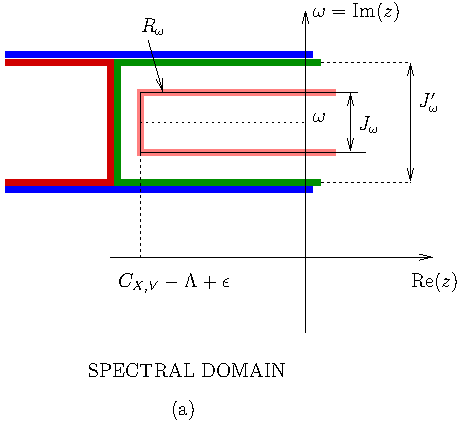
\includegraphics[scale=1]{figures/zones-1-a.pdf}}
\end{subfigure}
\hfill
\begin{subfigure}
{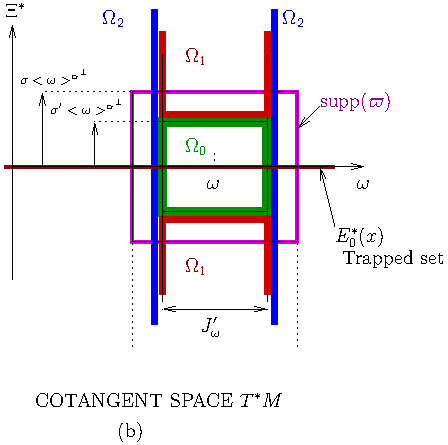
\includegraphics[scale=1]{figures/zones-1-b.pdf}}
\end{subfigure}
\caption{\textbf{(a)}: In the proof of Lemma~\ref{prop:discrete_spectrum}, we show that a perturbation $A'=A-\Lambda\Opp (\varpi)$ of the generator $A$ has no spectrum on the spectral domain $R_{\omega}\subset\bbC$ with frequency range $J_{\omega}=[\omega-1,\omega+1]$.\linebreak
\textbf{(b)}: The operator $\Opp (\varpi)$ is constructed from a compact vicinity $\supp(\varpi)$ of the trapped set $E_{0}^{*}\subset T^{*}M$ for a larger range of frequencies and with transverse size $\sigma\langle \omega\rangle ^{\alpha^{\perp}}$. We introduce a partition $T^{*}M=\Omega_{0}\cup\Omega_{1}\cup\Omega_{2}$ where $\Omega_{0}$ is a compact vicinity of the trapped set $E_{0}^{*}$ for an intermediate range of frequencies $J'_{\omega}$ and with transverse size $\sigma'\langle \omega\rangle ^{\alpha{}^{\perp}}$ so that $\Omega_{0}\subset\supp(\varpi)$. The set $\Omega_{1}$ is the outside of $\Omega_{0}$ (away from the trapped set) with the same frequencies range $J'_{\omega}$ and $\Omega_{2}$ are all the other points with other frequencies. During the proof, we take $\sigma\gg\sigma'\gg1$.}
\label{fig:zones}
\end{figure}

In order to construct $R_{r}(z)$ and $R_{l}(z)$, we take a real number $c>0$ and set
\begin{equation}\label{eq:def_J'}
J'_{\omega}:=\left[\omega-\left(1+c\right),\omega+\left(1+c\right)\right]\:\underset{\eqref{eq:def_J_omega}}{\supset}\:J{}_{\omega}.
\end{equation}
We take another constant $\sigma'>0$ and set $\Omega_{0}$ as a $K-$ball around the trapped set at frequency $\omega$:
\begin{multline}\label{eq:def_Omega_0}
\Omega_{0}:=\\
\left\{ \rho=\rho_{u}+\rho_{s}+\omega\alpha\left(m\right)\in T^{*}M,\,m=\pi\left(\rho\right)\in M,\omega\in J'_{\omega},\,\left\Vert \rho_{u}+\rho_{s}\right\Vert _{g_{\rho}}\leq K\right\},
\end{multline}
\begin{align}
\Omega_{1} &{:=}\left\{ \rho=\rho_{u}+\rho_{s}+\omega\alpha\left(m\right)\in T^{*}M,\,\omega\in J'_{\omega},\,\left\Vert \rho_{u}+\rho_{s}\right\Vert _{g_{\rho}}\geq K\right\}\label{eq:def_Omega_1}
\\
\intertext{and}
\Omega_{2} &{:=}\left\{ \rho\in T^{*}M,\quad\omega\left(\rho\right)\in\bbR\backslash J'_{\omega}\right\}\label{eq:def_Omega_2}
\end{align}
so that $T^{*}M=\Omega_{0}\cup\Omega_{1}\cup\Omega_{2}$. These regions are drawn on Figure~\ref{fig:zones} and explained in the caption. For $j=0,1,2$, let $\chi_{\Omega_{j}}$ be the characteristic function of $\Omega_{j}$. We have $\sum_{j}\chi_{\Omega_{j}}=1$ and hence
\begin{equation}\label{eq:ident}
\Id \underset{\eqref{eq:resol_ident_Pi_rho}}{=}\Opp \left(1\right)=\Opp \left(\chi_{\Omega_{0}}\right)+\Opp \left(\chi_{\Omega_{1}}\right)+\Opp \left(\chi_{\Omega_{2}}\right).
\end{equation}
Correspondingly to the decomposition~\eqref{eq:ident}, we will construct an approximate resolvent
\[
R_{r}\left(z\right)=R_{r}^{\left(0\right)}\left(z\right)+R_{r}^{\left(1\right)}\left(z\right)+R_{r}^{\left(2\right)}\left(z\right)
\]
with three contributions $R_{r}^{(j)}(z)$, $j=0,1,2$, so that each of them are uniformly bounded for $z\in R_{\omega}$ (and $\omega\in\bbR$) and satisfies
\begin{equation}\label{eq:approximate_R_j}
\left\Vert \left(z-A'\right)R_{r}^{\left(j\right)}\left(z\right)-\Opp \left(\chi_{\Omega_{j}}\right)\right\Vert _{\clH _{W}}\leq\frac{1}{6}.
\end{equation}
The estimate~\eqref{eq:approximate_R_j} will give~\eqref{eq:almost_inverse} and finish the proof of Lemma~\ref{lem:bounded_resolvent_of_A'}.

\paragraph{Contribution $R_{r}^{(0)}(z)$}\label{par:Contribution}

For the function $\varpi$ in~\eqref{eq:def_Omega_0'} and $t\geq0$, we define
\begin{equation}\label{eq:def_varpi_0-t}
\varpi_{\left[0,t\right]}:=\int_{0}^{t}\varpi\circ\tilde{\phi}^{s}ds.
\end{equation}
Let $T>0$ and\footnote{Let us explain why the expression~\eqref{eq:expression_R(0)} is a natural guess. Formally a good guess for the resolvent would be $R_{r}(z):=\int_{0}^{\infty}e^{-t(z-A')}dt$ with $A'=A-\Lambda\Opp (\varpi)$. However the operator $e^{tA'}$ has no clear mathematical sense but using Egorov's formula~\eqref{eq:norm_Egorov_PDO}, for bounded time, the operator $e^{tA'}$ is approximated by $e^{tA}e^{-\Opp (\varpi_{[0,t]})}$. Finally we truncate the integral up to a finite (but large) $T$ and compose with a final truncation operator $\Opp (\chi_{\Omega_{0}})$ to get~\eqref{eq:expression_R(0)}.}
\begin{equation}\label{eq:expression_R(0)}
R_{r}^{\left(0\right)}\left(z\right):=\int_{0}^{T}e^{-t\left(z-A\right)}\Opp \left(e^{-\Lambda\varpi_{\left[0,t\right]}}\right)\Opp \left(\chi_{\Omega_{0}}\right)dt.
\end{equation}
We assume that the constant $\sigma$ in~\eqref{eq:def_Omega_0'} is large enough so that we have
\[
\varpi\left(\tilde{\phi}^{t}\left(\rho\right)\right)=1\quad\text{and}\quad\varpi_{\left[0,t\right]}\left(\rho\right)\underset{\eqref{eq:def_varpi_0-t}}{=}t\quad\text{for all }t\in\left[0,T\right]\text{ and }\rho\in\Omega_{0}.
\]
We apply Corollary~\ref{cor:B3}, regarding $\sigma\geq1$ as the parameter, let $t\in[0,T]$, and see that for every $N>0$, there exists $C_{N,T}>0$ such that
\[
\left\Vert \Opp \left(e^{-\Lambda\varpi_{\left[0,t\right]}}\right)\Opp \left(\chi_{\Omega_{0}}\right)-e^{-t\Lambda}\Opp \left(\chi_{\Omega_{0}}\right)\right\Vert _{\clH _{W}}\underset{\eqref{eq:corollary_compos}}{\leq}C_{N,T}\sigma^{-N}.
\]
Since $\Vert \Opp (\chi_{\Omega_{0}})\Vert _{\clH _{W}}\leq1$ from~\eqref{eq:norme_symbol}, it follows that
\[
\left\Vert \Opp \left(e^{-\Lambda\varpi_{\left[0,t\right]}}\right)\Opp \left(\chi_{\Omega_{0}}\right)\right\Vert _{\clH _{W}}\leq e^{-t\Lambda}+C_{N,T}\sigma^{-N}.
\]
Therefore we have
\begin{equation}\label{eq:res5}
\begin{split}
\left\Vert e^{-t\left(z-A\right)}\Opp \left(e^{-\Lambda\varpi_{\left[0,t\right]}}\right)\Opp \left(\chi_{\Omega_{0}}\right)\right\Vert _{\clH _{W}} & \underset{\eqref{eq:bound_C_X,V}}{\leq}Ce^{-t\left(\Ree\left(z\right)-C_{X,V}+\Lambda\right)}+C_{N,T}\sigma^{-N}\\
& \mkern10mu\le Ce^{-t\epsilon}+C_{N,T}\sigma^{-N}
\end{split}
\end{equation}
for $t\in[0,T]$ and hence we deduce that, for $z\in R_{\omega}$,
\[
\left\Vert R_{r}^{\left(0\right)}\left(z\right)\right\Vert \underset{\eqref{eq:expression_R(0)}}{\leq}\int_{0}^{T}\left\Vert e^{-t\left(z-A\right)}\Opp \left(e^{-\Lambda\varpi_{\left[0,t\right]}}\right)\Opp \left(\chi_{\Omega_{0}}\right)\right\Vert _{\clH _{W}}dt\underset{\eqref{eq:res5}}{\leq}\frac{C}{\epsilon}+C{}_{N,T}\sigma{}^{-N}.
\]
Since the constant $C_{N,T}$ does not depend on $\sigma$, we can let the constant $\sigma$ be large for given $T>0$ so that the last term $C_{N,T}\sigma{}^{-N}$ is small relative to the former term $C/\epsilon$ and that the operator norm $\Vert R_{r}^{(0)}(z)\Vert $ is uniformly bounded for $z\in R_{\omega}$ (and $\omega\in\bbR$).

Now we prove the required estimate~\eqref{eq:approximate_R_j}. Observe that
\begin{multline}\label{eq:res1}
\frac{d}{dt}\left(e^{-t\left(z-A\right)}\Opp \left(e^{-\Lambda\varpi_{\left[0,t\right]}}\right)\right)  =\\
-\left(z-A\right)e^{-t\left(z-A\right)}\Opp \left(e^{-\Lambda\varpi_{\left[0,t\right]}}\right)
-e^{-t\left(z-A\right)}\Opp \left(\Lambda\varpi\circ\tilde{\phi}^{t}\cdot e^{-\Lambda\varpi_{\left[0,t\right]}}\right).
\end{multline}
For the last term of~\eqref{eq:res1}, we apply Theorem~\ref{thm:Composition-of-PDO.} on composition of PDO, Egorov's Theorem~\ref{thm:Egorov.-For-any} and also the slow variation property of $\varpi$ in~\eqref{eq:slow_variation_varpi} and obtain
\begin{multline*}
e^{-t\left(z-A\right)} \Opp \left(\Lambda\varpi\circ\tilde{\phi}^{t}\cdot e^{-\Lambda\varpi_{\left[0,t\right]}}\right)\\
\begin{aligned}
&\:\underset{\eqref{eq:norm_Compos_PDO}}{=}  e^{-t\left(z-A\right)}\Opp \left(\Lambda\varpi\circ\tilde{\phi}^{t}\right)\circ\Opp \left(e^{-\Lambda\varpi_{\left[0,t\right]}}\right)+O_{\clH _{W}}\left(C_{t}\sigma^{-1}\right)\\
&\underset{\eqref{eq:norm_Egorov_PDO}}{=}  \Lambda\Opp \left(\varpi\right)\circ e^{-t\left(z-A\right)}\circ\Opp \left(e^{-\Lambda\varpi_{\left[0,t\right]}}\right)+O_{\clH _{W}}\left(C_{t}\sigma^{-1}\right)
\end{aligned}
\end{multline*}
where $C_{t}>0$ depends on $t$ and the error term $O_{\clH _{W}}(C_{t}\sigma^{-1})$ denote an operator whose operator norm on $\clH _{W}$ is bounded by $C_{t}\sigma^{-1}$. Putting this estimate in~\eqref{eq:res1}, we get
\begin{multline}\label{eq:res3}
\frac{d}{dt}\left(e^{-t\left(z-A\right)}\Opp \left(e^{-\Lambda\varpi_{\left[0,t\right]}}\right)\right)\\
= -\left(z-A+\Lambda\Opp \left(\varpi\right)\right)e^{-t\left(z-A\right)}\Opp \left(e^{-\Lambda\varpi_{\left[0,t\right]}}\right)
+O_{\clH _{W}}\left(C_{t}\sigma^{-1}\right)
\end{multline}
Then we deduce that
\begin{multline}\label{eq:res}
\left(z-A'\right)\circ R_{r}^{\left(0\right)}\left(z\right)-\Opp \left(\chi_{\Omega_{0}}\right)\\
\begin{aligned}
&\mkern-17mu\underset{\eqref{eq:def_A'},\eqref{eq:expression_R(0)}}{=}\left(z-A+\Lambda\Opp \left(\varpi\right)\right)\int_{0}^{T}e^{-t\left(z-A\right)}\Opp \left(e^{-\Lambda\varpi_{\left[0,t\right]}}\right)\Opp \left(\chi_{\Omega_{0}}\right)dt-\Opp \left(\chi_{\Omega_{0}}\right)\\
& \underset{\eqref{eq:res3}}{=}-\int_{0}^{T}\frac{d}{dt}\left(e^{-t\left(z-A\right)}\Opp \left(e^{-\Lambda\varpi_{\left[0,t\right]}}\right)\right)\Opp \left(\chi_{\Omega_{0}}\right)dt+O_{\clH _{W}}\left(C_{T}\sigma^{-1}\right)-\Opp \left(\chi_{\Omega_{0}}\right)\\
& \mkern10mu =-e^{-T\left(z-A\right)}\Opp \left(e^{-\Lambda\varpi_{\left[0,T\right]}}\right)\Opp \left(\chi_{\Omega_{0}}\right)+O_{\clH _{W}}\left(C_{T}\sigma^{-1}\right)
\end{aligned}
\end{multline}
and hence that
\[
\left\Vert \left(z-A'\right)\circ R_{r}^{\left(0\right)}\left(z\right)-\Opp \left(\chi_{\Omega_{0}}\right)\right\Vert _{\clH _{W}}\underset{\eqref{eq:res},\eqref{eq:res5}}{\leq}Ce^{-T\epsilon}+C_{T}\sigma^{-1}.
\]
For a fixed $\epsilon>0$ and some given $N\geq1$ we take $T$ large enough and then $\sigma$ large enough depending on $T$ so that $\Vert (z-A')\circ R_{r}^{(0)}(z)-\Opp (\chi_{\Omega_{0}})\Vert _{\clH _{W}}\leq1/6$. This proves~\eqref{eq:approximate_R_j} for $j=0$.

\paragraph{Contribution $R_{r}^{(1)}(z)$}

We follow a construction similar to what we did for $R_{r}^{(0)}(z)$. Let $T>0$ and
\begin{equation}\label{eq:expression_R(1)}
R_{r}^{\left(1\right)}\left(z\right):=\int_{0}^{T}e^{-t\left(z-A\right)}\Opp \left(e^{-\Lambda\varpi_{\left[0,t\right]}}\right)\Opp \left(\chi_{\Omega_{1}}\right)dt.
\end{equation}

\pagebreak

By Theorem~\eqref{thm:decay_outside_trapped_set} applied to function $\chi_{\Omega_{1}}$ instead of $(1-\Lambda_{\sigma})$ (the proof is the same) we get that there exists $C>0$, for any $T>0$, $t\in[0,T]$, we can choose $h_{0}$ small enough and $\sigma$ and $K$ large enough so that
\begin{equation}\label{eq:res6}
\left\Vert e^{tA}\Opp \left(\chi_{\Omega_{1}}\right)\right\Vert _{\clH _{W}}\leq Ce^{\left(C_{X,V}-\Lambda+\epsilon'\right)t}.
\end{equation}
By using Egorov Theorem to permute the operators, we get
\begin{equation}\label{eq:egorov_R1}
e^{-t\left(z-A\right)}\Opp \left(e^{-\Lambda\varpi_{\left[0,t\right]}}\right)\underset{\eqref{eq:norm_Egorov_PDO}}{=}\Opp \left(e^{-\Lambda\varpi_{\left[-t,0\right]}}\right)e^{-t\left(z-A\right)}+O_{\clH _{W}}\left(C_{T}\sigma^{-1}\right).
\end{equation}
for $t\in[0,T]$. Since $\Vert \Opp (e^{-\Lambda\varpi_{[-T,0]}})\Vert _{\clH _{W}}\leq C$, we have
\begin{equation}\label{eq:res55}
\begin{split}
\left\Vert \Opp \left(e^{-\Lambda\varpi_{\left[-t,0\right]}}\right)e^{-t\left(z-A\right)}\Opp \left(\chi_{\Omega_{1}}\right)\right\Vert _{\clH _{W}} & \underset{\eqref{eq:res6}}{\leq}Ce^{-t\Ree\left(z\right)}e^{\left(C_{X,V}-\Lambda+\epsilon'\right)t}\\
& \underset{\eqref{eq:def_region_R}}{\leq}Ce^{-t\epsilon}.
\end{split}
\end{equation}
We deduce
\begin{align*}
\left\Vert R_{r}^{\left(1\right)}\left(z\right)\right\Vert & \underset{\eqref{eq:expression_R(1)},\,\eqref{eq:egorov_R1}}{\leq}\int_{0}^{T}\left\Vert \Opp \left(e^{-\Lambda\varpi_{\left[-t,0\right]}}\right)e^{-t\left(z-A\right)}\Opp \left(\chi_{\Omega_{1}}\right)\right\Vert dt+C_{T}\sigma^{-1}\\
& \mkern28mu\leq\frac{C}{\epsilon}+C_{T}\sigma^{-1}.
\end{align*}
Therefore $R_{r}^{(1)}(z)$ is bounded uniformly $z\in R_{\omega}$. Similarly to the case of $R_{r}^{(0)}(z)$, we have
\begin{multline}\label{eq:ress}
\left(z-A'\right)\circ R_{r}^{\left(1\right)}\left(z\right)-\Opp \left(\chi_{\Omega_{1}}\right)\\
\begin{aligned}
&= -e^{-T\left(z-A\right)}\Opp \left(e^{-\Lambda\varpi_{\left[0,T\right]}}\right)\Opp \left(\chi_{\Omega_{1}}\right)+O_{\clH _{W}}\left(C_{T}\sigma^{-1}\right)\\
&=  -\Opp \left(e^{-\Lambda\varpi_{\left[-T,0\right]}}\right)e^{-T\left(z-A\right)}\Opp \left(\chi_{\Omega_{1}}\right)+O_{\clH _{W}}\left(C_{T}\sigma^{-1}\right)
\end{aligned}
\end{multline}
and deduce
\[
\left\Vert \left(z-A'\right)\circ R_{r}^{\left(1\right)}\left(z\right)-\Opp \left(\chi_{\Omega_{1}}\right)\right\Vert _{\clH _{W}}\underset{\eqref{eq:ress},\eqref{eq:res55}}{\leq}Ce^{-T\epsilon}+C_{T}\sigma^{-1}.
\]
For a fixed $\epsilon>0$, we may take large $T$ and then take $h_{0}$ small and $\sigma$ large enough depending on $T$ so that $\Vert (z-A')\circ R_{r}^{(1)}(z)-\Opp (\chi_{\Omega_{0}})\Vert _{\clH _{W}}\leq\frac{1}{6}$. We have obtained~\eqref{eq:approximate_R_j} for $j=1$.


\paragraph{Contribution $R_{r}^{(2)}(z)$}

On the domain $\Omega_{2}$ we will use ``elliptic estimate'' techniques. The symplectic volume $m$ on $T^{*}M$ naturally induces the conditional measure $m_{\omega}$ on each of the level set $\boldsymbol{\omega}{}^{-1}(\omega)$ so that $m=\int m_{\omega}d\omega$. For each $\omega'\in\bbR$, we define
\begin{equation}\label{eq:def_Pi_omega}
\Pi\left(\omega'\right):=\int\Pi\left(\rho'\right)\frac{dm_{\omega}}{\left(2\pi\right)^{n+1}}.
\end{equation}
Let
\begin{align*}
R_{r}^{\left(2\right)}\left(z\right) &{:=}\int_{\omega'\notin J'}\frac{1}{z-i\omega'}\Pi\left(\omega'\right)d\omega'\\
& \mkern-28mu\underset{\eqref{eq:def_Pi_omega},\eqref{eq:def_Omega_2}}{=}\int_{\Omega_{2}}\frac{1}{z-i\omega\left(\rho'\right)}\Pi\left(\rho'\right)\frac{d\rho'}{\left(2\pi\right)^{n+1}}\\
& \mkern-11mu\eq{\ref{eq:def_operator}}\Opp \left(\frac{1}{z-i\omega\left(.\right)}\mathrm{1}_{\Omega_{2}}\right)
\end{align*}

Since $\max_{\omega\,\notin\,J'}|\frac{1}{z-i\omega}|\leq c^{-1}$, we deduce from Theorem~\ref{thm:Continuity-of-PDO} that
\begin{equation}\label{eq:norm_B}
\left\Vert R_{r}^{\left(2\right)}\left(z\right)\right\Vert _{\clH _{W}}\le Cc^{-1},
\end{equation}
where $C$ does not depend on $\omega,z$.

\begin{lemm}\label{lem:bound_norm_D}
We have
\begin{equation}\label{eq:norm_D}
\left\Vert \left(z-A'\right)R_{r}^{\left(2\right)}\left(z\right)-\Opp \left(\chi_{\Omega_{2}}\right)\right\Vert _{\clH _{W}}^{2}\le Cc^{-1}.
\end{equation}
where the constant $C$ depends on $\Lambda$ and $V$.
\end{lemm}

Then taking $c$ large enough proves~\eqref{eq:approximate_R_j} for $j=2$.
\begin{proof}
We write first
\begin{multline}\label{eq:A'}
\left(z-A'\right)R_{r}^{\left(2\right)}\left(z\right)-\Opp \left(\chi_{\Omega_{2}}\right)\\
\begin{aligned}
& =\int_{\Omega_{2}}\frac{z-A'}{z-i\omega\left(\rho\right)}\Pi\left(\rho\right)\frac{d\rho}{\left(2\pi\right)^{n+1}}-\int_{\Omega_{2}}\Pi\left(\rho\right)\frac{d\rho}{\left(2\pi\right)^{n+1}}\\
& =\int_{\Omega_{2}}\frac{z-A'-\left(z-i\omega\left(\rho\right)\right)}{z-i\omega\left(\rho\right)}\Pi\left(\rho\right)\frac{d\rho}{\left(2\pi\right)^{n+1}}\\
& =-\int_{\Omega_{2}}\frac{A'-i\omega\left(\rho\right)}{z-i\omega\left(\rho\right)}\Pi\left(\rho\right)\frac{d\rho}{\left(2\pi\right)^{n+1}}\\
& =-\int_{\omega'\notin J'}\frac{A'-i\omega'}{z-i\omega'}\Pi\left(\omega'\right)d\omega'.
\end{aligned}
\end{multline}
We have
\[
A'\eq{\ref{eq:def_A'}}A-\Lambda\cdot\Opp \left(\varpi\right)\eq{\ref{eq:generator_A}}-X+V-\Lambda\cdot\Opp \left(\varpi\right).
\]
We have seen in~\eqref{eq:symbol_X} that $-X=\Opp (i\omega)+R$ with a remainder $R\in\Psi(\langle|\rho|\rangle^{\alpha^{\parallel}})$, here $\alpha^{\parallel}=0$. Then $R=A'-\Opp (i\omega)\in\Psi(1)$ as well, since $V,\Lambda\varpi$ are bounded. We write
\begin{multline*}
\int_{\omega'\notin J'}\frac{A'-i\omega'}{z-i\omega'}\Pi\left(\omega'\right)d\omega'\\
=\left(\Opp \left(i\omega\left(.\right)\right)+R\right)\Opp \left(\frac{1}{z-i\omega\left(.\right)}\mathrm{1}_{\Omega_{2}}\right)+\Opp \left(\frac{-i\omega\left(.\right)}{z-i\omega\left(.\right)}\mathrm{1}_{\Omega_{2}}\right).
\end{multline*}
By the composition Theorem~\ref{thm:Composition-of-PDO.}, using that $\omega(.)$ is slowly varying with function $h(\rho)=(\delta^{\parallel}(\rho))^{-1}=1$, and since $\max_{\omega\,\notin\,J'}|\frac{1}{z-i\omega}|\leq c^{-1}$, we have
\[
\Opp \left(i\omega\left(.\right)\right)\Opp \left(\frac{1}{z-i\omega\left(.\right)}\mathrm{1}_{\Omega_{2}}\right)=\Opp \left(\frac{i\omega\left(.\right)}{z-i\omega\left(.\right)}\mathrm{1}_{\Omega_{2}}\right)+\Psi\left(r_{2}\right)
\]
with $r_{2}=h(\rho)c^{-1}=c^{-1}$. Also
\begin{align*}
R\Opp \left(\frac{1}{z-i\omega\left(.\right)}\mathrm{1}_{\Omega_{2}}\right) &\in\Psi\left(c^{-1}\right),
\\
\intertext{hence}
\int_{\omega'\,\notin\,J'}\frac{A'-i\omega'}{z-i\omega'}\Pi\left(\omega'\right)d\omega' &\in\Psi\left(c^{-1}\right).
\end{align*}
From Theorem~\ref{thm:Continuity-of-PDO} we deduce that $\Vert \int_{\omega'\,\notin\,J'}\frac{A'-i\omega'}{z-i\omega'}\Pi(\omega')d\omega'\Vert _{\clH _{W}}\leq Cc^{-1}$. With~\eqref{eq:A'}, we deduce~\eqref{eq:norm_D}.
\end{proof}

\section{Proof of Theorem~\ref{thm:WF} and Corollary~\ref{cor:Let-us-choose} about the wave front set}\label{sec:Proof-of-Theorem_WF}

\subsection{Proof of Theorem~\ref{thm:WF}}

Let $g$ be an admissible metric. $\clT:C^{\infty}(M;\bbC)\rightarrow\clS(T^{*}M;\bbC^{J})$ denotes the wave-packet transform~\eqref{eq:def_T_in-1} constructed from that metric $g$. Let $W$ be an escape function as defined in Lemma~\ref{thm:W} and $\clH _{W}\left(M\right)$ be the anisotropic Sobolev space defined from $W$ in~\eqref{eq:def_H_W}.

Consider a discrete eigenvalue $z_{0}\in\bbC$ of the generator $A=-X+V$ with $\Ree(z_{0})>C_{X,V}-\Lambda$ and we set $\omega_{0}=\Imm(z_{0})$. Assume that $u\in\clH _{W}\left(M\right)$ is a generalized eigenvector for the eigenvalue $z_{0}$, that is to say
\begin{equation}\label{eq:Aku}
\left(A-z_{0}\right)^{k}u=0
\end{equation}
for some $k\in\bbN$, $k\geq1$. We assume $\Ree z_{0}>a$, for some $a\in\bbR$. The estimates will be uniform in $\omega_{0}$ but non uniform in $a$.

Let us define a function $f\in C^{\infty}\left(T^{*}M;\bbC\right)$
\[
f\left(\rho\right)=\left(i\left(\omega-\omega_{0}\right)\right)^{-k},
\]
with $\omega=\boldsymbol{\omega}(\rho)$, when $|\omega-\omega_{0}|\geq1$ and bounded by $1$ when $|\omega-\omega_{0}|\leq1$. Let $R$ be the operator defined by
\begin{equation}\label{eq:def_R-2}
R:=\Id -\Opp (f)(A-z_{0})^{k}.
\end{equation}
Using the notation of Definition~\ref{def:Let--be-1} for $\Psi$, we have the following estimate.
\begin{lem}
For any $m>0$,
\begin{equation}\label{eq:Rm}
R^{m}\in\Psi\left(\left\langle \boldsymbol{\omega}-\omega_{0}\right\rangle ^{-m}\left\langle \left|\rho\right|\right\rangle ^{m\alpha^{\parallel}}\right).
\end{equation}
\end{lem}

\begin{proof}
Recall from~\eqref{eq:symbol_X} that
\[
\left(A-\Opp \left(i\boldsymbol{\omega}\right)\right)\in\Psi\left(\left\langle \left|\rho\right|\right\rangle ^{\alpha^{\parallel}}\right)
\]
Also uniformly in $\omega_{0}$ we have that
\begin{align*}
\left(\left(A-z_{0}\right)^{k}-\Opp \left(\left(i\boldsymbol{\omega}-z_{0}\right)^{k}\right)\right) &\in\Psi\left(\left|\boldsymbol{\omega}-\omega_{0}\right|^{k-1}\left\langle \left|\rho\right|\right\rangle ^{\alpha^{\parallel}}\right)
\\
\left(\left(A-z_{0}\right)^{k}-\Opp \left(f^{-1}\right)\right)&\in\Psi\left(\left|\boldsymbol{\omega}-\omega_{0}\right|^{k-1}\left\langle \left|\rho\right|\right\rangle ^{\alpha^{\parallel}}\right)
\end{align*}
From composition theorem:
\[
\Opp \left(f\right)\Opp \left(f^{-1}\right)-\Id \in\Psi\left(\left|\boldsymbol{\omega}-\omega_{0}\right|^{-1}\left\langle \left|\rho\right|\right\rangle ^{\alpha^{\parallel}}\right)
\]
Thus
\begin{align*}
R  \eq{\ref{eq:def_R-2}}&\Id -\Opp \left(f\right)\Opp \left(f^{-1}\right)+\Opp \left(f\right)\left(\Opp \left(f^{-1}\right)-\left(A-z_{0}\right)^{k}\right)\\
& \in\Psi\left(\left|\boldsymbol{\omega}-\omega_{0}\right|^{-1}\left\langle \left|\rho\right|\right\rangle ^{\alpha^{\parallel}}\right).
\end{align*}
and~\eqref{eq:Rm} follows.
\end{proof}

We have $Ru\underset{\eqref{eq:Aku},\eqref{eq:def_R-2}}{=}u$ hence for any $m\geq1$,
\begin{equation}\label{eq:Tu}
\left(\clT u\right)\left(\rho'\right)=\left(\clT R^{m}\clT^{\dagger}\clT u\right)\left(\rho'\right)=\int\langle\delta_{\rho',j'}|\clT R^{m}\clT^{\dagger}\delta_{\rho,j}\rangle\left(\clT u\right)\left(\rho\right)\frac{d\rho}{\left(2\pi\right)^{n+1}}
\end{equation}
Therefore for $\rho\in T^{*}M$,
\begin{multline*}
W\left(\rho'\right)\left|\left(\clT u\right)\left(\rho'\right)\right|\\
\begin{aligned}
& \ineq{\ref{eq:Tu}}W\left(\rho'\right)\sum_{j,j'}\int\left|\left\langle\delta_{\rho',j'}\,\middle|\,\clT R^{m}\clT^{\dagger}\delta_{\rho,j}\right\rangle\right|\left|\left(\clT u\right)\left(\rho\right)\right|\frac{d\rho}{\left(2\pi\right)^{n+1}}\\
& \mkern-20mu\underset{\eqref{eq:Rm},\eqref{eq:microl_estimate-2}}{\leq}W\left(\rho'\right)\frac{C_{N,m}}{\left\langle \omega'-\omega_{0}\right\rangle ^{m}}\left\langle \left|\rho'\right|\right\rangle ^{m\alpha^{\parallel}}\int\left\langle \dist_{g}\left(\rho',\rho\right)\right\rangle ^{-N}\left|\left(\clT u\right)\left(\rho\right)\right|\frac{d\rho}{\left(2\pi\right)^{n+1}}\\
& \mkern-3mu\ineq{\ref{eq:slow_variation_W}}\frac{C_{N,m}\left\langle \left|\rho'\right|\right\rangle ^{m\alpha^{\parallel}}}{\left\langle \omega'-\omega_{0}\right\rangle ^{m}}\int\left\langle \dist_{g}\left(\rho',\rho\right)\right\rangle ^{-N}W\left(\rho\right)\left|\left(\clT u\right)\left(\rho\right)\right|\frac{d\rho}{\left(2\pi\right)^{n+1}}\\
& \mkern-5mu\ineq{\mathrm{C.S.}}\frac{C_{N,m}\left\langle \left|\rho'\right|\right\rangle ^{m\alpha^{\parallel}}}{\left\langle \omega'-\omega_{0}\right\rangle ^{m}}\left(\int\left\langle \dist_{g}\left(\rho',\rho\right)\right\rangle ^{-2N}\frac{d\rho}{\left(2\pi\right)^{n+1}}\right)^{1/2}\\
& \qquad\left(\int\left(W\left(\rho\right)\right)^{2}\left|\left(\clT u\right)\left(\rho\right)\right|^{2}\frac{d\rho}{\left(2\pi\right)^{n+1}}\right)^{1/2}\\
& \mkern-07mu\underset{\eqref{eq:def_Sobolev_norm}}{\leq}\frac{C_{m}\left\langle \left|\rho'\right|\right\rangle ^{m\alpha^{\parallel}}}{\left\langle \omega'-\omega_{0}\right\rangle ^{m}}\left\Vert u\right\Vert _{\clH _{W}\left(M\right)}
\end{aligned}
\end{multline*}
or
\begin{equation}\label{eq:res-1-1}
\left|\left(\clT u\right)\left(\rho'\right)\right|\leq\frac{C_{m}\left\langle \left|\rho'\right|\right\rangle ^{m\alpha^{\parallel}}}{W\left(\rho'\right)\left\langle \omega'-\omega_{0}\right\rangle ^{m}}\left\Vert u\right\Vert _{\clH _{W}\left(M\right)}.
\end{equation}
We have obtained the claim~\eqref{eq:WF-1-1} of the Theorem~\ref{thm:WF}.

\subsection{\label{subsec:Proof-of-Corollary}
Proof of Corollary~\ref{cor:Let-us-choose}}

We choose a phase space metric $g$ as defined in~\eqref{eq:metric_g_in_coordinates} with the following parameters
\[
\alpha^{\perp}=\frac{1}{1+\min\left(\beta_{u},\beta_{s}\right)},\quad\alpha^{\parallel}=0.
\]
Let $C>0$. We choose a weight function $W$ as in Lemma~\ref{thm:W}, with parameter $R_{s},R_{u}>0$ large enough to reveal the discrete spectrum on $\Ree(z)\geq-C$ and $R_{s}$ will be taken larger later. We choose parameters $\gamma=0$. For $\rho\in T^{*}M$, we write $\rho=\omega\scrA+\rho_{s}+\rho_{u}$ with $\omega\in\bbR$, $\rho_{u}\in E_{u}^{*}$, $\rho_{s}\in E_{s}^{*}$. Then
\begin{align*}
W\left(\rho\right)\left\langle \omega-\omega_{0}\right\rangle ^{m} & \underset{\eqref{eq:def_W1}}{=}\frac{\left\langle h_{0}\left\Vert \rho_{s}\right\Vert _{g_{\rho}}\right\rangle ^{R_{s}}}{\left\langle h_{0}\left\Vert \rho_{u}\right\Vert _{g_{\rho}}\right\rangle ^{R_{u}}}\left\langle \omega-\omega_{0}\right\rangle ^{m}\underset{\eqref{eq:def_norm_g}}{=}\frac{\left\langle h_{0}\left|\rho\right|^{-\alpha^{\perp}}\left|\rho_{s}\right|\right\rangle ^{R_{s}}}{\left\langle h_{0}\left|\rho\right|^{-\alpha^{\perp}}\left|\rho_{u}\right|\right\rangle ^{R_{u}}}\left\langle \omega-\omega_{0}\right\rangle ^{m}\\
& \mkern13mu\geq\left\langle \left|\rho\right|\right\rangle ^{-R_{u}\left(1-\alpha^{\perp}\right)}\left\langle h_{0}\left|\rho\right|^{-\alpha^{\perp}}\left|\rho_{s}\right|\right\rangle ^{R_{s}}\left\langle \omega-\omega_{0}\right\rangle ^{m}.
\end{align*}
Let $\epsilon>0$ and assume $\rho\in T^{*}M\backslash\clV_{\omega_{0},\epsilon}$ where $\clV_{\omega_{0},\epsilon}$ is defined in~\eqref{eq:Vu}. This means that
\[
\left\langle \omega-\omega_{0}\right\rangle \geq\left|\rho\right|^{\epsilon}\quad\text{ or }\quad\left\langle \left|\rho\right|^{-\alpha^{\perp}}\left|\rho_{s}\right|\right\rangle \geq\left|\rho\right|^{\epsilon}.
\]
Let $N\geq1$. If $\langle \omega-\omega_{0}\rangle \geq|\rho|^{\epsilon}$, we choose $m$ large enough so that $m\epsilon-R_{u}(1-\alpha^{\perp})\geq N$ and hence that
\[
W\left(\rho\right)\left\langle \omega-\omega_{0}\right\rangle ^{m}\geq\left\langle \left|\rho\right|\right\rangle ^{-R_{u}\left(1-\alpha^{\perp}\right)}\left\langle \omega-\omega_{0}\right\rangle ^{m}\geq C_{N,\epsilon}\left\langle \left|\rho\right|\right\rangle ^{m\epsilon-R_{u}\left(1-\alpha^{\perp}\right)}\geq C_{N,\epsilon}\left\langle \rho\right\rangle ^{N}.
\]
If $\langle |\rho|^{-\alpha^{\perp}}|\rho_{s}|\rangle \geq|\rho|^{\epsilon}$, we choose $R_{s}$ large enough so that $R_{s}\epsilon-R_{u}(1-\alpha^{\perp})\geq N$ and hence that
\begin{align*}
W\left(\rho\right)\left\langle \omega-\omega_{0}\right\rangle ^{m}&\geq\left\langle \left|\rho\right|\right\rangle ^{-R_{u}\left(1-\alpha^{\perp}\right)}\left\langle \left|\rho\right|^{-\alpha^{\perp}}\left|\rho_{s}\right|\right\rangle ^{R_{s}}\\
&\geq C_{N,\epsilon}\left\langle \left|\rho\right|\right\rangle ^{R_{s}\epsilon-R_{u}\left(1-\alpha^{\perp}\right)}\geq C_{N,\epsilon}\left\langle \rho\right\rangle ^{N}.
\end{align*}
In both cases, we obtain that
\[
\left|\left(\clT u\right)\left(\rho\right)\right|\underset{\eqref{eq:res-1-1}}{\leq}\frac{C_{m}}{W\left(\rho\right)\left\langle \omega-\omega_{0}\right\rangle ^{m}}\left\Vert u\right\Vert _{\clH _{W}\left(M\right)}\leq\frac{C_{N,\epsilon}}{\left\langle \rho\right\rangle ^{N}}\left\Vert u\right\Vert _{\clH _{W}\left(M\right)}.
\]
This finishes the proof of Corollary~\ref{cor:Let-us-choose}.
\clearpage

\appendix

\section{Proof of Theorem~\ref{thm:W} about properties of \texorpdfstring{$W$}{W}}\label{subsec:Proof-of-Thm}

\subsection{Definition of the escape function \texorpdfstring{$W$}{W}}

The escape function $W:T^{*}M\rightarrow\bbR^{+}$ has been defined in~\eqref{eq:def_W1}. Here, we will first give an other equivalent definition of $W$ in~\eqref{eq:def_W} that will be more convenient for the proof of Theorem~\ref{thm:W}.

%\subsubsection*{Definition of map $\Phi_{j}$}
For a point $m\in M$, we have defined the decomposition of a cotangent vector 
\[
\rho\eq{\ref{eq:decomp_Xi}}\rho_{u}+\rho_{s}+\rho_{0}\in T_{m}^{*}M,\quad\text{where}\quad\rho_{u}\in E_{u}^{*}(m),\rho_{s}\in E_{s}^{*}(m),\rho_{0}\in E_{0}^{*}(m).
\]
Recall from~\eqref{eq:def_E_u*} and~\eqref{eq:Holder_exp} that the map $m\in M\mapsto E_{\sigma}^{*}(m)$, $\sigma=u,s,0$, are H\"older continuous with respective exponent $\beta_{u},\beta_{s},\beta_{0}$. Consequently the decomposition $\rho=\rho_{u}+\rho_{s}+\rho_{0}$ is continuous but not smooth.

We have taken a global smooth metric $g_{M}$ on $M$ and we denote $\Vert.\Vert _{g_{M}}$ the induced norm on $T^{*}M$. From $g_{M}$ we define a new metric $\tilde{g}_{M}$ on $M$ as follows. The metric $\tilde{g}_{M}$ equals $g_{M}$ on $E_{\sigma}^{*}$ for $\sigma=u,s,0$ and the sum $E_{u}^{*}\oplus E_{s}^{*}\oplus E_{0}^{*}$ is orthogonal for $\tilde{g}_{M}$. As a consequence $\tilde{g}_{M}$ is H\"older continuous on $M$.

Let $\kappa_{j}:U_{j}\subset M\rightarrow V_{j}\subset\bbR_{x,z}^{n+1}$ a local chart diffeomorphism on $M$ as defined in~\eqref{eq:def_kappa_j} and $\tilde{\kappa}_{j}:T^{*}U_{j}\subset T^{*}M\rightarrow T^{*}V_{j}\subset T^{*}\bbR^{n+1}$ the lifted map on cotangent space defined in~\eqref{eq:def_k_tilde_j}. There exists a continuous linear bundle map over $\Id $ of the form
\begin{equation}\label{eq:def_Phi}
\Phi_{j}:
\begin{cases}
T^{*}V_{j} & \rightarrow T^{*}\left(\bbR^{n}\times\bbR\right)\\
\left(\left(x,z\right),\left(\xi,\omega\right)\right) & \mapsto\left(\left(x,z\right),\left(\tilde{\xi},\omega\right)\right)
\end{cases}
\end{equation}
with
\begin{equation}\label{eq:xi_tilde}
\tilde{\xi}=A\left(x\right)\xi+\omega B\left(x\right)\in\bbR^{n}
\end{equation}
such that:
\begin{enumerate}
\item $\Phi_{j}\circ\tilde{\kappa}_{j}$ maps $E_{u}^{*}\oplus E_{s}^{*}\oplus E_{0}^{*}$ to $\bbR^{d_{u}}\oplus\bbR^{d_{s}}\oplus\bbR$, with $d_{u}+d_{s}=n$. For this, $A(x):\bbR^{n}\rightarrow\bbR^{n}$ is a linear invertible map that depends continuously on $x\in\bbR^{n}$ with H\"older exponent $\beta_{*}=\min\{\beta_{s},\beta_{u}\}$ and $B(x)\in\bbR^{n}$ depends continuously on $x\in\bbR^{n}$ with H\"older exponent $\beta_{0}$.
\item For any $\rho=\rho_{u}+\rho_{s}+\rho_{0}\in E_{u}^{*}\oplus E_{s}^{*}\oplus E_{0}^{*}=T^{*}M$,
\begin{equation}\label{eq:prop_Phi}
\left|\left(\Phi_{j}\circ\tilde{\kappa}_{j}\right)\left(\rho_{\sigma}\right)\right|=\left\Vert \rho_{\sigma}\right\Vert _{\tilde{g}_{M}},\quad\text{for }\sigma=u,s,0,
\end{equation}
where $|.|$ denotes the Euclidean canonical norm on $\bbR^{n+1}$.
\end{enumerate}
From $\tilde{g}_{M}$-orthogonality of the decomposition $E_{u}^{*}\oplus E_{s}^{*}\oplus E_{0}^{*}$ and orthogonality of $\bbR^{d_{u}}\oplus\bbR^{d_{s}}\oplus\bbR$ for the Euclidean metric, we have that
\begin{equation}\label{eq:prop_Phi_1}
\forall\rho\in T^{*}M,\quad\left|\left(\Phi_{j}\circ\tilde{\kappa}_{j}\right)\left(\rho\right)\right|=\left\Vert \rho\right\Vert _{\tilde{g}_{M}}.
\end{equation}


%\subsubsection*{Definition of the function $\tilde{W}$}

We define the metric $\tilde{g}$ on $\bbR^{n+1}$ as follows. Let $\tilde{\eta}=(\tilde{\xi},\omega)\in\bbR^{n}\times\bbR$. For $\tilde{v}=(\tilde{v}_{\xi},\tilde{v}_{\omega})\in T_{\tilde{\eta}}(\bbR^{n}\times\bbR)$,
\begin{equation}\label{eq:norm_g}
\left\Vert \tilde{v}\right\Vert _{\tilde{g}\left(\tilde{\eta}\right)}^{2}=\left(\left\langle \left|\tilde{\eta}\right|\right\rangle ^{-\alpha^{\perp}}\left|\tilde{v}_{\xi}\right|\right)^{2}+\left(\left\langle \left|\tilde{\eta}\right|\right\rangle ^{-\alpha^{\parallel}}\left|\tilde{v}_{\omega}\right|\right)^{2}.
\end{equation}
Let $0<\gamma<1$. We define the function $\tilde{h}_{\gamma}^{\perp}:\bbR^{n+1}\rightarrow\bbR^{+}$ as follows.
\begin{equation}\label{eq:h_tilde}
\tilde{h}_{\gamma}^{\perp}\left(\tilde{\eta}\right)=\left\langle \left\Vert \tilde{\xi}\right\Vert _{\tilde{g}\left(\tilde{\eta}\right)}\right\rangle ^{-\gamma}\underset{\eqref{eq:norm_g}}{=}\left\langle \left\langle \left|\tilde{\eta}\right|\right\rangle ^{-\alpha^{\perp}}\left|\tilde{\xi}\right|\right\rangle ^{-\gamma}.
\end{equation}
We define the function $\tilde{W}:\bbR^{n+1}\rightarrow\bbR^{+}$ as follows. With $\tilde{\xi}=(\tilde{\xi}{}_{u},\tilde{\xi}{}_{s})\in\bbR^{d_{u}}\times\bbR^{d_{s}}=~\bbR^{n}$,
\begin{equation}\label{eq:def_W_tilde}
\tilde{W}\left(\tilde{\eta}\right):=\frac{\left\langle h_{0}\tilde{h}_{\gamma}^{\perp}\left(\tilde{\eta}\right)\left\Vert \tilde{\xi}{}_{s}\right\Vert _{\tilde{g}\left(\tilde{\eta}\right)}\right\rangle ^{R_{s}}}{\left\langle h_{0}\tilde{h}_{\gamma}^{\perp}\left(\tilde{\eta}\right)\left\Vert \tilde{\xi}{}_{u}\right\Vert _{\tilde{g}\left(\tilde{\eta}\right)}\right\rangle ^{R_{u}}}.
\end{equation}

\begin{rema}
Let us observe from~\eqref{eq:prop_Phi_1} that for $\rho\in T^{*}U_{j}\cap T^{*}U_{j'}$ we have $\tilde{W}\circ\Phi_{j}\circ\tilde{\kappa}_{j}(\rho)=\tilde{W}\circ\Phi_{j'}\circ\tilde{\kappa}_{j'}(\rho)$, i.e. this expression is independent on chart.
\end{rema}


%\subsubsection*{The global function $W$}

\begin{cBoxB}{}
\begin{lemm}[Alternative expression of the escape function $W$]
The function $W:T^{*}U_{j}\subset T^{*}M\rightarrow\bbR^{+}$ defined in~\eqref{eq:def_W1} can be expressed using the function $\tilde{W}$ in~\eqref{eq:def_W_tilde} as follows:
\begin{equation}\label{eq:def_W}
W=\left(\boldsymbol{1}_{y}\otimes\tilde{W}\right)\circ\Phi_{j}\circ\tilde{\kappa}_{j},
\end{equation}
where $\boldsymbol{1}_{y}:y=(x,z)\in\bbR^{n+1}\rightarrow1\in\bbR$ is the constant unit function on the variables of position.
\end{lemm}
\end{cBoxB}

\begin{proof}
We check that $W$ in~\eqref{eq:def_W} coincides with the function $W$ given in~\eqref{eq:def_W1}. Essentially this is due to Definition~\eqref{eq:norm_g-1} that we have used for the metric $\tilde{g}(\rho)$.
\end{proof}

\subsection{The slowly varying and temperate property~\eqref{enu:-satisfies--temperate-1}}

Here, we will prove that the function $W$ satisfies~\eqref{eq:slow_variation_W}. For this, we use the expression~\eqref{eq:def_W} that expresses the function $W$ as a smooth function $\boldsymbol{1}_{y}\otimes\tilde{W}$ constant on the base, composed with the function $\Phi_{j}$. In the first step, we will prove that the smooth function $\tilde{W}$ satisfies the slowly varying and temperate property. In a second step, we will show that $\Phi_{j}$ has the property of being Lipschitz at scale greater than~$1$. We will then deduce that the slowly varying and temperate property holds true for~$W$.

\subsubsection{The slowly varying and temperate property for \texorpdfstring{$\tilde{W}$}{W}}

The next proposition gives the temperate property and slow variation property of $\tilde{W}$ defined in~\eqref{eq:def_W_tilde}, that corresponds to the Claim~\ref{enu:-satisfies--temperate-1} of Theorem~\ref{thm:W} (but for $\tilde{W}$).

\begin{cBoxB}{}
\begin{prop}
Assume that $\alpha^{\perp},\alpha^{\parallel}$ and $0\leq\gamma<1$ are given and satisfy the relations~\eqref{eq:ineq1} and~\eqref{eq:gamma_interval}. Then there exist constants $N_{\tilde{W}}>0$, $C_{\tilde{W}}$ and $0<\mu<1$ such that for every $h_{0}>0$,
\begin{align}\label{eq:w2}
\frac{\tilde{W}(\tilde{\eta}')}{\tilde{W}(\tilde{\eta})}\le1+C_{\tilde{W}}h_{0}^{\mu}\left\langle\tilde{h}_{\gamma}^{\perp}\left(\tilde{\eta}\right)\left\|\tilde{\eta}'-\tilde{\eta}\right\|_{\tilde{g}\left(\tilde{\eta}\right)}\right\rangle^{N_{\tilde{W}}}\quad\text{for all }\tilde{\eta},\tilde{\eta}'\in\bbR^{n+1}.
\end{align}
\end{prop}
\end{cBoxB}

\begin{proof}
For simplicity of notation, we define the conformal metric $\tilde{g}_{\gamma}$ on $T\bbR^{n+1}$ as follows. We write for $\tilde{v}\in T_{\tilde{\eta}}\bbR^{n+1}$
\begin{equation}\label{eq:def_gtilde}
\left\Vert \tilde{v}\right\Vert _{\tilde{g}_{\gamma}\left(\tilde{\eta}\right)}:=\tilde{h}_{\gamma}^{\perp}\left(\tilde{\eta}\right)\left\Vert \tilde{v}\right\Vert _{\tilde{g}\left(\tilde{\eta}\right)}.
\end{equation}
Consider expression~\eqref{eq:def_W_tilde} of $\tilde{W}$. For the proof of the proposition, it is enough to show the estimates
\begin{align}\label{eq:reducedclaim1}
\max\left\{ \frac{\left\langle h_{0}\|\tilde{\xi}'_{s}\|_{\tilde{g}_{\gamma}\left(\tilde{\eta}'\right)}\right\rangle}{\left\langle h_{0}\|\tilde{\xi}_{s}\|_{\tilde{g}_{\gamma}\left(\tilde{\eta}\right)}\right\rangle},\frac{\left\langle h_{0}\|\tilde{\xi}_{s}\|_{\tilde{g}_{\gamma}\left(\tilde{\eta}\right)}\right\rangle}{\left\langle h_{0}\|\tilde{\xi}'_{s}\|_{\tilde{g}_{\gamma}\left(\tilde{\eta}'\right)}\right\rangle}\right\} \le1+Ch_{0}^{\mu}\left\langle\|\tilde{\eta}'-\tilde{\eta}|_{\tilde{g}_{\gamma}\left(\tilde{\eta}\right)}\right\rangle^{N}
\end{align}
and the corresponding claims with $\tilde{\xi}_{s}$ and $\tilde{\xi}'_{s}$ replaced by $\tilde{\xi}_{u}$ and $\tilde{\xi}'_{u}$ respectively. We give a proof of the claim~\eqref{eq:reducedclaim1}. The proof of the other claim is parallel. We will choose the small constant $\mu>0$ in the due course and the choice may be implicit in the following argument.

Note that, if $\|\tilde{\xi}\|_{\tilde{g}_{\gamma}(\tilde{\eta})}\le h_{0}^{-\delta}$ and $\|\tilde{\xi}'\|_{\tilde{g}_{\gamma}(\tilde{\eta}')}\le h_{0}^{-\delta}$ with some $0<\delta<1$, then
\[
h_{0}\|\tilde{\xi}_{s}\|_{\tilde{g}_{\gamma}\left(\tilde{\eta}\right)}\le h_{0}^{1-\delta}<1
\]
and the same estimate for $\|\tilde{\xi}'_{s}\|_{\tilde{g}_{\gamma}(\tilde{\eta})}$. Then the required estimate~\eqref{eq:reducedclaim1} is trivial because the function $x\mapsto\langle x\rangle$ is almost flat around the origin $0$. Therefore we may assume either $\|\tilde{\xi}\|_{\tilde{g}_{\gamma}(\tilde{\eta})}>h_{0}^{-\delta}$ or $\|\tilde{\xi}'\|_{\tilde{g}_{\gamma}(\tilde{\eta}')}>h_{0}^{-\delta}$. Below we assume
\begin{equation}\label{eq:hdelta}
\|\tilde{\xi}\|_{\tilde{g}_{\gamma}\left(\tilde{\eta}\right)}>h_{0}^{-\delta}.
\end{equation}
As we will explain at the end, the claim in the other case follows immediately if we are done with this case. Note that
\begin{equation}\label{eq:eta}
|\tilde{\eta}|\ge\|\tilde{\eta}\|_{\tilde{g}\left(\tilde{\eta}\right)}\ge\|\tilde{\xi}\|_{\tilde{g}\left(\tilde{\eta}\right)}\ge\|\tilde{\xi}\|_{\tilde{g}_{\gamma}\left(\tilde{\eta}\right)}\underset{\eqref{eq:hdelta}}{>}h_{0}^{-\delta}.
\end{equation}
We have
\begin{multline}\label{eq:basic}
\max\left\{ \frac{\left\langle h_{0}\|\tilde{\xi}'_{s}\|_{\tilde{g}_{\gamma}\left(\tilde{\eta}\right)}\right\rangle}{\left\langle h_{0}\|\tilde{\xi}_{s}\|_{\tilde{g}_{\gamma}\left(\tilde{\eta}\right)}\right\rangle},\frac{\left\langle h_{0}\|\tilde{\xi}_{s}\|_{\tilde{g}_{\gamma}\left(\tilde{\eta}\right)}\right\rangle}{\left\langle h_{0}\|\tilde{\xi}'_{s}\|_{\tilde{g}_{\gamma}\left(\tilde{\eta}\right)}\right\rangle}\right\}\\
\ineq{\ref{eq:D1p}}1+h_{0}\left|\|\tilde{\xi}'_{s}\|_{\tilde{g}_{\gamma}\left(\tilde{\eta}\right)}-\|\tilde{\xi}{}_{s}\|_{\tilde{g}_{\gamma}\left(\tilde{\eta}\right)}\right|\le1+h_{0}\|\tilde{\xi}'_{s}-\tilde{\xi}_{s}\|_{\tilde{g}_{\gamma}\left(\tilde{\eta}\right)}.
\end{multline}
Hence, for the proof of the claim~\eqref{eq:reducedclaim1}, we compare the metric $\tilde{g}_{\gamma}(\tilde{\eta})$ and $\tilde{g}_{\gamma}(\tilde{\eta}')$.

Recall from Lemma~\ref{lem:temperate_metric} that the metric $g$ hence $\tilde{g}$ also, is $\Delta^{\gamma}$-moderate that is, with the distortion function 
\[
\Delta(\tilde{\eta})\eq{\ref{eq:def_distortion_function_D-1}}\langle|\tilde{\eta}|\rangle^{-(1-\alpha^{\perp})},
\]
we have that, for arbitrary $0\neq v\in\real^{n+1}$,
\begin{equation}\label{claim1}
\max\left\{ \frac{\|v\|_{\tilde{g}\left(\tilde{\eta}'\right)}}{\|v\|_{\tilde{g}\left(\tilde{\eta}\right)}},\frac{\|v\|_{\tilde{g}\left(\tilde{\eta}\right)}}{\|v\|_{\tilde{g}\left(\tilde{\eta}'\right)}}\right\} \le1+C\Delta(\tilde{\eta})^{1-\gamma}\left\langle \Delta(\tilde{\eta})^{\gamma}\cdot\|\tilde{\eta}'-\tilde{\eta}\|_{\tilde{g}\left(\tilde{\eta}\right)}\right\rangle ^{N}.
\end{equation}
For $0<\lambda<1$, $x\in\bbR$, we have
\begin{equation}\label{eq:ineq-1}
\lambda\left\langle x\right\rangle \leq\left\langle \lambda x\right\rangle.
\end{equation}
We have
\begin{align}
\tilde{h}_{\gamma}^{\perp}(\tilde{\eta})\underset{\eqref{eq:h_tilde}}{\geq}\langle\langle|\tilde{\eta}|\rangle^{-\alpha^{\perp}}|\tilde{\eta}|\rangle^{-\gamma}\underset{\eqref{eq:ineq-1}}{\geq}\langle|\tilde{\eta}|\rangle^{-\gamma\left(1-\alpha^{\perp}\right)}&\eq{\ref{eq:def_distortion_function_D-1}}\Delta(\tilde{\eta})^{\gamma},\label{eq:*3}
\\
\intertext{and}
\Delta(\tilde{\eta})^{1-\gamma}=\langle|\tilde{\eta}|\rangle^{-\left(1-\gamma\right)\left(1-\alpha^{\perp}\right)}\ineq{\ref{eq:eta}}Ch_{0}^{\delta\left(1-\gamma\right)\left(1-\alpha^{\perp}\right)} &\mkern5mu =Ch_{0}^{\mu}\label{eq:*3b}
\end{align}
with $\mu=(1-\gamma)(1-\alpha^{\perp})<1$. We get that, for arbitrary $0\neq v\in\real^{n+1}$,
\begin{align}\label{claim3}
\max\left\{ \frac{\|v\|_{\tilde{g}\left(\tilde{\eta}\right)}}{\|v\|_{\tilde{g}\left(\tilde{\eta}'\right)}},\frac{\|v\|_{\tilde{g}\left(\tilde{\eta}'\right)}}{\|v\|_{\tilde{g}\left(\tilde{\eta}\right)}}\right\} \underset{\eqref{claim1},\eqref{eq:*3},\eqref{eq:*3b}}{\leq} & 1+Ch_{0}^{\mu}\cdot\left\langle \|\tilde{\eta}'-\tilde{\eta}\|_{\tilde{g}_{\gamma}\left(\tilde{\eta}\right)}\right\rangle ^{N}.
\end{align}

To get~\eqref{eq:reducedclaim1}, we want to extend the estimate~\eqref{claim3} to the case where the metric $\tilde{g}$ on the left hand side is replaced by the metric $\tilde{g}_{\gamma}$. To this end, we have to estimate the ratio between $\tilde{h}_{\gamma}^{\perp}(\tilde{\eta})$ and $\tilde{h}_{\gamma}^{\perp}(\tilde{\eta}')$. We have
\begin{multline}\label{eq:vg}
\max  \left\{ \frac{\tilde{h}_{\gamma}^{\perp}(\tilde{\eta}')}{\tilde{h}_{\gamma}^{\perp}(\tilde{\eta})},\frac{\tilde{h}_{\gamma}^{\perp}(\tilde{\eta})}{\tilde{h}_{\gamma}^{\perp}(\tilde{\eta}')}\right\}\\
\begin{aligned}
&\mkern-10mu\eq{\ref{eq:h_tilde}}\max\left\{ \frac{\left\langle\|\tilde{\xi}'\|_{\tilde{g}\left(\tilde{\eta}'\right)}\right\rangle}{\left\langle\|\tilde{\xi}\|_{\tilde{g}\left(\tilde{\eta}\right)}\right\rangle},\frac{\left\langle\|\tilde{\xi}\|_{\tilde{g}\left(\tilde{\eta}\right)}\right\rangle}{\left\langle\|\tilde{\xi}'\|_{\tilde{g}\left(\tilde{\eta}'\right)}\right\rangle}\right\} ^{\gamma}\\
& \le\max\left\{ \frac{\left\langle\|\tilde{\xi}'\|_{\tilde{g}\left(\tilde{\eta}\right)}\right\rangle}{\left\langle\|\tilde{\xi}\|_{\tilde{g}\left(\tilde{\eta}\right)}\right\rangle}\cdot\frac{\left\langle\|\tilde{\xi}'\|_{\tilde{g}\left(\tilde{\eta}'\right)}\right\rangle}{\left\langle\|\tilde{\xi}'\|_{\tilde{g}\left(\tilde{\eta}\right)}\right\rangle},\frac{\left\langle\|\tilde{\xi}\|_{\tilde{g}\left(\tilde{\eta}\right)}\right\rangle}{\left\langle\|\tilde{\xi}'\|_{\tilde{g}\left(\tilde{\eta}\right)}\right\rangle}\cdot\frac{\left\langle\|\tilde{\xi}'\|_{\tilde{g}\left(\tilde{\eta}\right)}\right\rangle}{\left\langle\|\tilde{\xi}'\|_{\tilde{g}\left(\tilde{\eta}'\right)}\right\rangle}\right\} ^{\gamma}\\
& \le\max\left\{ \frac{\left\langle\|\tilde{\xi}'\|_{\tilde{g}\left(\tilde{\eta}\right)}\right\rangle}{\left\langle\|\tilde{\xi}\|_{\tilde{g}\left(\tilde{\eta}\right)}\right\rangle},\frac{\left\langle\|\tilde{\xi}\|_{\tilde{g}\left(\tilde{\eta}\right)}\right\rangle}{\left\langle\|\tilde{\xi}'\|_{\tilde{g}\left(\tilde{\eta}\right)}\right\rangle}\right\}^{\gamma}\cdot\max\left\{ \frac{\left\langle\|\tilde{\xi}'\|_{\tilde{g}\left(\tilde{\eta}'\right)}\right\rangle}{\left\langle\|\tilde{\xi}'\|_{\tilde{g}\left(\tilde{\eta}\right)}\right\rangle},\frac{\left\langle\|\tilde{\xi}'\|_{\tilde{g}\left(\tilde{\eta}\right)}\right\rangle}{\left\langle\|\tilde{\xi}'\|_{\tilde{g}\left(\tilde{\eta}'\right)}\right\rangle}\right\} ^{\gamma}.
\end{aligned}
\end{multline}
And, for the second term on the right-hand side of~\eqref{eq:vg}, we apply~\eqref{claim3} and see
\begin{equation}\label{hgamma1}
\max\left\{ \frac{\left\langle\|\tilde{\xi}'\|_{\tilde{g}\left(\tilde{\eta}'\right)}\right\rangle}{\left\langle\|\tilde{\xi}'\|_{\tilde{g}\left(\tilde{\eta}\right)}\right\rangle},\frac{\left\langle\|\tilde{\xi}'\|_{\tilde{g}\left(\tilde{\eta}\right)}\right\rangle}{\left\langle\|\tilde{\xi}'\|_{\tilde{g}\left(\tilde{\eta}'\right)}\right\rangle}\right\} \le1+Ch_{0}^{\mu}\cdot\left\langle \|\tilde{\eta}'-\tilde{\eta}\|_{\tilde{g}_{\gamma}\left(\tilde{\eta}\right)}\right\rangle ^{N}.
\end{equation}
For the first term on the right-hand side of~\eqref{eq:vg}, we consider two cases separately:
\begin{enumerate}
\item In the case where $\|\tilde{\xi}'-\tilde{\xi}\|_{\tilde{g}(\tilde{\eta})}\leq\frac{1}{2}\|\tilde{\xi}\|_{\tilde{g}(\tilde{\eta})}$ we have
\begin{equation}
\|\tilde{\xi}'\|_{\tilde{g}\left(\tilde{\eta}\right)}\ge\|\tilde{\xi}\|_{\tilde{g}\left(\tilde{\eta}\right)}-\|\tilde{\xi}'-\tilde{\xi}\|_{\tilde{g}\left(\tilde{\eta}\right)}\ge\|\tilde{\xi}\|_{\tilde{g}\left(\tilde{\eta}\right)}/2\underset{\eqref{eq:eta}}{>}h_{0}^{-\delta}/2\label{eq:*4}
\end{equation}
and hence, using (D.1), we see
\begin{align}
\max\left\{ \frac{\left\langle\|\tilde{\xi}'\|_{\tilde{g}\left(\tilde{\eta}\right)}\right\rangle}{\left\langle\|\tilde{\xi}\|_{\tilde{g}\left(\tilde{\eta}\right)}\right\rangle},\frac{\left\langle\|\tilde{\xi}\|_{\tilde{g}\left(\tilde{\eta}\right)}\right\rangle}{\left\langle\|\tilde{\xi}'\|_{\tilde{g}\left(\tilde{\eta}\right)}\right\rangle}\right\} & \ineq{\ref{eq:D1p}}1+\frac{\|\tilde{\xi}'-\tilde{\xi}\|_{\tilde{g}\left(\tilde{\eta}\right)}}{\min\left\{\left\langle\|\tilde{\xi}\|_{\tilde{g}\left(\tilde{\eta}\right)}\right\rangle,\left\langle\|\tilde{\xi}'\|_{\tilde{g}\left(\tilde{\eta}\right)}\right\rangle\right\}}\label{eq:log}
\\
& \!\ineq{\ref{eq:*4}}1+\frac{2\|\tilde{\xi}'-\tilde{\xi}\|_{\tilde{g}\left(\tilde{\eta}\right)}}{\langle\|\tilde{\xi}\|_{\tilde{g}\left(\tilde{\eta}\right)}\rangle}\label{eq:*10}
\end{align}
Since $\tilde{h}_{\gamma}^{\perp}(\tilde{\eta})=\langle\|\tilde{\xi}\|_{\tilde{g}(\tilde{\eta})}\rangle^{-\gamma}$, we continue
\begin{align}\label{eq:log3}
\max\left\{ \frac{\left\langle\|\tilde{\xi}'\|_{\tilde{g}\left(\tilde{\eta}\right)}\right\rangle}{\left\langle\|\tilde{\xi}\|_{\tilde{g}\left(\tilde{\eta}\right)}\right\rangle},\frac{\left\langle\|\tilde{\xi}\|_{\tilde{g}\left(\tilde{\eta}\right)}\right\rangle}{\left\langle\|\tilde{\xi}'\|_{\tilde{g}\left(\tilde{\eta}\right)}\right\rangle}\right\} & \ineq{\ref{eq:*10}}1+2\left\langle\|\tilde{\xi}\|_{\tilde{g}\left(\tilde{\eta}\right)}\right\rangle^{-(1-\gamma)}\|\tilde{\xi}'-\tilde{\xi}\|_{\tilde{g}_{\gamma}\left(\tilde{\eta}\right)}
\\
& \mkern9mu\le1+Ch_{0}^{\mu}\left\langle\|\tilde{\xi}'-\tilde{\xi}\|_{\tilde{g}_{\gamma}\left(\tilde{\eta}\right)}\right\rangle.
\end{align}
where $\mu=\delta(1-\gamma)<1$ because $\langle\|\tilde{\xi}\|_{\tilde{g}(\tilde{\eta})}\rangle^{-(1-\gamma)}\ineq{\ref{eq:eta}}h_{0}^{\delta(1-\gamma)}$.
\item In the case where $\|\tilde{\xi}'-\tilde{\xi}\|_{\tilde{g}(\tilde{\eta})}>\frac{1}{2}\|\tilde{\xi}\|_{\tilde{g}(\tilde{\eta})}$ we have
\begin{align}\label{eq:*5}
\begin{split}
\|\tilde{\xi}'-\tilde{\xi}\|_{\tilde{g}_{\gamma}\left(\tilde{\eta}\right)} & \eq{\ref{eq:def_gtilde}}\tilde{h}_{\gamma}^{\perp}(\tilde{\eta})\|\tilde{\xi}'-\tilde{\xi}\|_{\tilde{g}\left(\tilde{\eta}\right)}=\left\langle\|\tilde{\xi}\|_{g_{\tilde{\eta}}}\right\rangle^{-\gamma}\cdot\|\tilde{\xi}'-\tilde{\xi}\|_{\tilde{g}\left(\tilde{\eta}\right)}\\
& \mkern3mu\underset{(\mathrm{Hyp.})}{\geq}C^{-1}\left\langle\|\tilde{\xi}'-\tilde{\xi}\|_{\tilde{g}\left(\tilde{\eta}\right)}\right\rangle^{1-\gamma}.
\end{split}
\end{align}
Note also that the assumption~\eqref{eq:eta} gives
\begin{equation}
\|\tilde{\xi}'-\tilde{\xi}\|_{\tilde{g}\left(\tilde{\eta}\right)}>\|\tilde{\xi}\|_{\tilde{g}\left(\tilde{\eta}\right)}/2>h_{0}^{-\delta}/2\quad\text{and hence}\quad2h_{0}^{\delta}\|\tilde{\xi}'-\tilde{\xi}\|_{\tilde{g}\left(\tilde{\eta}\right)}>1\label{eq:a}
\end{equation}
From this estimate, we obtain
\begin{equation}\label{log2}
\begin{split}
\max\left\{ \frac{\left\langle\|\tilde{\xi}'\|_{\tilde{g}\left(\tilde{\eta}\right)}\right\rangle}{\left\langle\|\tilde{\xi}\|_{\tilde{g}\left(\tilde{\eta}\right)}\right\rangle},\frac{\left\langle\|\tilde{\xi}\|_{\tilde{g}\left(\tilde{\eta}\right)}\right\rangle}{\left\langle\|\tilde{\xi}'\|_{\tilde{g}\left(\tilde{\eta}\right)}\right\rangle}\right\} & \ineq{\ref{eq:D1p}}1+\|\tilde{\xi}'-\tilde{\xi}\|_{\tilde{g}\left(\tilde{\eta}\right)}
\\
& \ineq{\ref{eq:a}}1+2h_{0}^{\delta}\|\tilde{\xi}'-\tilde{\xi}\|_{\tilde{g}\left(\tilde{\eta}\right)}^{2}\\
& \ineq{\ref{eq:*5}}1+2h_{0}^{\delta}\cdot\left\langle\|\tilde{\xi}'-\tilde{\xi}\|_{\tilde{g}_{\gamma}\left(\tilde{\eta}\right)}\right\rangle^{2/(1-\gamma)}\\
& \mkern13mu\le1+Ch_{0}^{\delta}\left\langle\|\tilde{\xi}'-\tilde{\xi}\|_{\tilde{g}\left(\tilde{\eta}\right)^{\gamma}}\right\rangle^{N}
\end{split}
\end{equation}
where, in the last inequality, we let $N>2/(1-\gamma)$.
\end{enumerate}
From~\eqref{eq:log3} and~\eqref{log2} in the two (exhaustive) cases, we always have
\[
\max\left\{ \frac{\left\langle\|\tilde{\xi}'\|_{\tilde{g}\left(\tilde{\eta}\right)}\right\rangle}{\left\langle\|\tilde{\xi}\|_{\tilde{g}\left(\tilde{\eta}\right)}\right\rangle},\frac{\left\langle\|\tilde{\xi}\|_{\tilde{g}\left(\tilde{\eta}\right)}\right\rangle}{\left\langle\|\tilde{\xi}'\|_{\tilde{g}\left(\tilde{\eta}\right)}\right\rangle}\right\} \le1+Ch_{0}^{\mu}\left\langle \|\tilde{\eta}'-\tilde{\eta}\|_{\tilde{g}_{\gamma}\left(\tilde{\eta}\right)}\right\rangle ^{N}
\]
for some constant $C>0$ and $N>0$. Plugging this inequality and~\eqref{hgamma1} in~\eqref{eq:vg}, we obtain
\[
\max\left\{ \frac{\tilde{h}_{\gamma}^{\perp}(\tilde{\eta}')}{\tilde{h}_{\gamma}^{\perp}(\tilde{\eta})},\frac{\tilde{h}_{\gamma}^{\perp}(\tilde{\eta})}{\tilde{h}_{\gamma}^{\perp}(\tilde{\eta}')}\right\} \le1+C'h_{0}^{\mu}\left\langle \|\tilde{\eta}'-\tilde{\eta}\|_{\tilde{g}_{\gamma}\left(\tilde{\eta}\right)}\right\rangle ^{N'}
\]
for some constant $C'>0$ and $N'>0$. From the last inequality and~\eqref{claim3}, we obtain, for any $0\neq v\in\real^{n+1}$, that
\begin{align}
\max\left\{ \frac{\|v\|_{\tilde{g}_{\gamma}\left(\tilde{\eta}\right)}}{\|v\|_{\tilde{g}_{\gamma}\left(\tilde{\eta}'\right)}},\frac{\|v\|_{\tilde{g}_{\gamma}\left(\tilde{\eta}'\right)}}{\|v\|_{\tilde{g}_{\gamma}\left(\tilde{\eta}\right)}}\right\} & \le1+C''h_{0}^{\mu}\cdot\left\langle \|\tilde{\eta}'-\tilde{\eta}\|_{\tilde{g}_{\gamma}\left(\tilde{\eta}\right)}\right\rangle ^{N''}\label{claim4}
\end{align}
for some $C''>1$ and $N''>1$.

Now we can conclude the claim~\eqref{eq:reducedclaim1}. Indeed, we have
\begin{align*}
\frac{\left\langle h_{0}\|\tilde{\xi}'_{s}\|_{\tilde{g}_{\gamma}\left(\tilde{\eta}'\right)}\right\rangle}{\left\langle h_{0}\|\tilde{\xi}_{s}\|_{\tilde{g}_{\gamma}\left(\tilde{\eta}\right)}\right\rangle} & =\frac{\left\langle h_{0}\|\tilde{\xi}'_{s}\|_{\tilde{g}_{\gamma}\left(\tilde{\eta}'\right)}\right\rangle}{\left\langle h_{0}\|\tilde{\xi}'_{s}\|_{\tilde{g}_{\gamma}\left(\tilde{\eta}\right)}\right\rangle}\frac{\left\langle h_{0}\|\tilde{\xi}'_{s}\|_{\tilde{g}_{\gamma}\left(\tilde{\eta}\right)}\right\rangle}{\left\langle h_{0}\|\tilde{\xi}_{s}\|_{\tilde{g}_{\gamma}\left(\tilde{\eta}\right)}\right\rangle}\\
& \le\frac{\left\langle\|\tilde{\xi}'_{s}\|_{\tilde{g}_{\gamma}\left(\tilde{\eta}'\right)}\right\rangle}{\left\langle\|\tilde{\xi}'_{s}\|_{\tilde{g}_{\gamma}\left(\tilde{\eta}\right)}\right\rangle}\frac{\left\langle h_{0}\|\tilde{\xi}'_{s}\|_{\tilde{g}_{\gamma}\left(\tilde{\eta}\right)}\right\rangle}{\left\langle h_{0}\|\tilde{\xi}_{s}\|_{\tilde{g}_{\gamma}\left(\tilde{\eta}\right)}\right\rangle}
\end{align*}
and we can apply~\eqref{claim4} for the former term on the right hand side and~\eqref{eq:basic} to the latter to get
\begin{align*}
\frac{\left\langle h_{0}\|\tilde{\xi}'_{s}\|_{\tilde{g}_{\gamma}\left(\tilde{\eta}'\right)}\right\rangle}{\left\langle h_{0}\|\tilde{\xi}_{s}\|_{\tilde{g}_{\gamma}\left(\tilde{\eta}\right)}\right\rangle} & \le \left(1+C''h_{0}^{\mu}\cdot\left\langle \|\tilde{\eta}'-\tilde{\eta}\|_{\tilde{g}_{\gamma}\left(\tilde{\eta}\right)}\right\rangle ^{N''}\right)\cdot\left(1+h_{0}\|\tilde{\xi}'_{s}-\tilde{\xi}_{s}\|_{\tilde{g}_{\gamma}\left(\tilde{\eta}\right)}\right)\\
& \le1+C_{*}h_{0}^{\mu}\cdot\left\langle \|\tilde{\eta}'-\tilde{\eta}\|_{\tilde{g}_{\gamma}\left(\tilde{\eta}\right)}\right\rangle ^{N_{*}}
\end{align*}
for some $C_{*},N_{*}>1$. Likewise, we obtain the same inequality for the reciprocal of the left-hand side, concluding the claim~\eqref{eq:reducedclaim1}.

Consider the remaining case where we have $\|\tilde{\xi}'\|_{\tilde{g}_{\gamma}(\tilde{\eta}')}>h_{0}^{-\delta}$ instead of $\|\tilde{\xi}\|_{\tilde{g}_{\gamma}(\tilde{\eta})}\linebreak >h_{0}^{-\delta}$ in~\eqref{eq:eta}. Then we can follow the argument above with $\tilde{\eta}$ and $\tilde{\eta}'$ exchanged and obtain
\begin{equation}\label{eq:reducedclaim2}
\max\left\{ \frac{\left\langle h_{0}\|\tilde{\xi}'_{s}\|_{\tilde{g}_{\gamma}\left(\tilde{\eta}'\right)}\right\rangle}{\left\langle h_{0}\|\tilde{\xi}_{s}\|_{\tilde{g}_{\gamma}\left(\tilde{\eta}\right)}\right\rangle},\frac{\left\langle h_{0}\|\tilde{\xi}_{s}\|_{\tilde{g}_{\gamma}\left(\tilde{\eta}\right)}\right\rangle}{\left\langle h_{0}\|\tilde{\xi}'_{s}\|_{\tilde{g}_{\gamma}\left(\tilde{\eta}'\right)}\right\rangle}\right\} \le1+Ch_{0}^{\mu}\left\langle\|\tilde{\eta}'-\tilde{\eta}\|_{\tilde{g}_{\gamma}\left(\tilde{\eta}'\right)^{\gamma}}\right\rangle^{N}.
\end{equation}
(The difference from~\eqref{eq:reducedclaim1} is only that the metric $\tilde{g}_{\gamma}(\tilde{\eta})$ is replaced by $\tilde{g}_{\gamma}(\tilde{\eta}')$ on the right-hand side.) Then from the temperate property~\eqref{eq:g_moderate and temperate} in Lemma~\ref{lem:temperate_metric}, we obtain the claim~\eqref{eq:reducedclaim1}.
\end{proof}

\subsubsection{The straightening coordinates are Lipschitz at scale greater than \texorpdfstring{$1$}{1}}

In~\eqref{eq:norm_g} we have defined an Euclidean scalar product $\tilde{g}$ on $T_{\tilde{\eta}}\bbR^{n+1}\equiv\bbR^{n+1}$ with coordinates $\tilde{\eta}=(\tilde{\xi},\omega)\in\bbR^{n+1}$. Here we extend this metric $\tilde{g}$ to a metric denoted $\overset{\thickapprox}{g}$ on $\bbR^{2\left(n+1\right)}$ with coordinates
\[
\tilde{\varrho}=\left(y,\tilde{\eta}\right)=\left(x,z,\tilde{\xi},\omega\right)\in\bbR^{2\left(n+1\right)},
\]
by simply adding the same Euclidean scalar product along $(x,z)$ as in~\eqref{eq:metric_g_in_coordinates}:
\begin{equation}\label{eq:def_g_double_tilde}
\overset{\thickapprox}{g}:=\left(\left\langle \tilde{\eta}\right\rangle ^{\alpha^{\perp}}dx\right)^{2}+\left(\left\langle \tilde{\eta}\right\rangle ^{\alpha^{\parallel}}dz\right)^{2}+\tilde{g},
\end{equation}
so that in coordinates $\overset{\thickapprox}{g}$ coincides with the metric $g$ in~\eqref{eq:metric_g_in_coordinates}. As in~\eqref{eq:def_gtilde} we define a conformal (or re-scaled) metric $\overset{\thickapprox}{g}_{\gamma}$ as follows. For $\tilde{v}\in T_{\tilde{\varrho}}\bbR^{2(n+1)}$,
\begin{equation}\label{eq:def_gtilde-1}
\left\Vert \tilde{v}\right\Vert _{\overset{\thickapprox}{g}_{\gamma}\left(\tilde{\varrho}\right)}=\tilde{h}_{\gamma}^{\perp}\left(\tilde{\eta}\right)\left\Vert \tilde{v}\right\Vert _{\overset{\thickapprox}{g}\left(\tilde{\varrho}\right)}.
\end{equation}
The following proposition shows that the map $\Phi_{j}$ is H\"older continuous and also Lipschitz in the scale greater than $1$ for the metric $\overset{\thickapprox}{g}_{\gamma}$.

\begin{cBoxB}{}
\begin{prop}
With the assumption~\eqref{eq:gamma_interval} on $0\leq\gamma<1$, the map $\Phi_{j}$ defined in~\eqref{eq:def_Phi} satisfies the following estimate: $\exists C>0$, $\forall\varrho,\varrho'\in T^{*}V_{j}\subset\bbR^{2(n+1)}$
\begin{equation}\label{eq:Phi_Lipchitz}
\begin{split}
\left\|\Phi_{j}(\varrho')-\Phi_{j}(\varrho)\right\|_{\overset{\thickapprox}{g}_{\gamma}\left(\Phi_{j}\left(\varrho\right)\right)} & \le C\max\left\{ \|\varrho'-\varrho\|_{\overset{\thickapprox}{g}_{\gamma}\left(\varrho\right)},\|\varrho'-\varrho\|_{\overset{\thickapprox}{g}_{\gamma}\left(\varrho\right)}^{\beta_{*}}\right\} 
\\
& \le C\left\langle\|\varrho'-\varrho\|_{\overset{\thickapprox}{g}_{\gamma}\left(\varrho\right)}\right\rangle.
\end{split}
\end{equation}
Consequently, over a chart $U_{j}\subset M$, $\exists C>0$, $\forall\rho,\rho'\in T^{*}U_{j}$ we have
\begin{align}\label{eq:Phi_Lipchitz-1}
\|\Phi_{j}\circ\tilde{\kappa}_{j}\left(\rho'\right)-\Phi_{j}\circ\tilde{\kappa}_{j}\left(\rho\right)\|_{\overset{\thickapprox}{g}_{\gamma}\left(\Phi_{j}\circ\tilde{\kappa}_{j}\left(\rho\right)\right)} & \le C\langle h_{\gamma}^{\perp}\left(\rho\right)\|\rho'-\rho\|_{g\left(\rho\right)}\rangle.
\end{align}
\end{prop}
\end{cBoxB}

\begin{proof}
Take two points
\[
\varrho=(y,\eta)=(x,z,\xi,\omega),\quad\varrho'=(y',\eta')=(x',z',\xi',\omega')\in\bbR^{2\left(n+1\right)}
\]
that satisfy
\[
d:=\|\varrho'-\varrho\|_{\overset{\thickapprox}{g}_{\gamma}\left(\varrho\right)}>0.
\]
From the definition of $\overset{\thickapprox}{g}_{\gamma}$ in~\eqref{eq:def_gtilde-1},\eqref{eq:def_g_double_tilde} and~\eqref{eq:norm_g}, this implies that
\begin{align*}
|x'-x|\le d\langle\eta\rangle^{-\alpha^{\perp}}, &\quad|z'-z|\le d\langle\eta\rangle^{-\alpha^{\parallel}},\\
|\xi'-\xi|\le d\langle\eta\rangle^{\alpha^{\perp}}\cdot h_{\gamma}^{\perp}(\eta)^{-1},&\quad|\omega'-\omega|\le d\langle\eta\rangle^{\alpha^{\parallel}}.
\end{align*}
We set
\[
\Phi_{j}(\varrho)=(y,\tilde{\eta})=(x,z,\tilde{\xi},\omega),\quad\Phi_{j}(\varrho')=(y',\tilde{\eta}')=(x',z',\tilde{\xi}',\omega').
\]
with $\tilde{\xi},\tilde{\xi}'$ given as in~\eqref{eq:xi_tilde}. Then we have
\[
|\tilde{\xi}'-\tilde{\xi}|\le C|\xi'-\xi|+C|\xi||x'-x|^{\beta_{*}}+C|\omega||x'-x|^{\beta_{0}}
\]
and also
\[
C^{-1}\langle\eta\rangle\le\langle\tilde{\eta}\rangle\le C\langle\eta\rangle.
\]
We will use that
\begin{equation}\label{eq:*7}
h_{\gamma}^{\perp}(\eta)\eq{\ref{eq:h_gamma}}\left\langle \left\Vert \xi\right\Vert _{g\left(\eta\right)}\right\rangle ^{-\gamma}=\left\langle \left\langle \left|\eta\right|\right\rangle ^{-\alpha^{\perp}}\left|\xi\right|\right\rangle ^{-\gamma}\leq\left\langle \left|\xi\right|^{1-\alpha^{\perp}}\right\rangle ^{-\gamma}\leq C\left\langle \left|\xi\right|\right\rangle ^{-\gamma\left(1-\alpha^{\perp}\right)}
\end{equation}
and $\gamma<1<\frac{1}{1-\alpha^{\perp}}$ to get that $1-\gamma(1-\alpha^{\perp})>0$ hence
\begin{equation}\label{eq:*8} 
\left\langle \xi\right\rangle ^{1-\gamma\left(1-\alpha^{\perp}\right)}\leq\left\langle \eta\right\rangle ^{1-\gamma\left(1-\alpha^{\perp}\right)}
\end{equation}

Hence
\begin{align*}
\left\|\Phi_{j}(\varrho')-\Phi_{j}(\varrho)\right\|_{\overset{\thickapprox}{g}_{\gamma}\left(\Phi_{j}\left(\varrho\right)\right)} & \le\langle\tilde{\eta}\rangle^{\alpha^{\perp}}|x'-x|+\langle\tilde{\eta}\rangle^{\alpha^{\parallel}}|z'-z|\\
& \quad+h_{\gamma}^{\perp}(\xi)\cdot\langle\tilde{\eta}\rangle^{-\alpha^{\perp}}\cdot|\tilde{\xi}'-\tilde{\xi}|+\langle\eta\rangle^{-\alpha^{\parallel}}|\omega'-\omega|\\
& \le Cd+Ch_{\gamma}^{\perp}(\xi)\cdot\langle\eta\rangle^{-\alpha^{\perp}}|\xi|\cdot\left(d\langle\eta\rangle^{-\alpha^{\perp}}\right)^{\beta_{*}}\\
& \quad+C\langle\eta\rangle^{-\alpha^{\perp}}|\omega|\left(d\langle\eta\rangle^{-\alpha^{\perp}}\right)^{\beta_{0}}\\
& \ineq{\ref{eq:*7}}Cd+C\langle\xi\rangle^{1-\gamma\left(1-\alpha^{\perp}\right)}\langle\eta\rangle^{-\left(1+\beta_{*}\right)\alpha^{\perp}}d^{\beta_{*}}\\
& \quad+C\langle\eta\rangle^{1-\alpha^{\perp}-\alpha^{\perp}\beta_{0}}d^{\beta_{0}}\\
& \ineq{\ref{eq:*8}}Cd+C\langle\eta\rangle^{1-\gamma(1-\alpha^{\perp})-(1+\beta_{*})\alpha^{\perp}}d^{\beta_{*}}\\
& \quad+C\langle\eta\rangle^{1-\alpha^{\perp}-\alpha^{\perp}\beta_{0}}d^{\beta_{0}}.
\end{align*}
We have from~\eqref{eq:gamma_interval}
\begin{align*}
\gamma\underset{\eqref{eq:gamma_interval}}{\geq}\frac{1-\alpha^{\perp}\left(1+\beta_{*}\right)}{1-\alpha^{\perp}}
\Leftrightarrow  1-\gamma\left(1-\alpha^{\perp}\right)-\left(1+\beta_{*}\right)\alpha^{\perp}\leq0,
\end{align*}
and also $1-\alpha^{\perp}(1+\beta_{0})<0$ from~\eqref{eq:ineq1}. We obtain that
\[
\left\|\Phi_{j}(\varrho')-\Phi_{j}(\varrho)\right\|_{\overset{\thickapprox}{g}_{\gamma}\left(\Phi_{j}\left(\varrho\right)\right)}\le C\left(d+d^{\beta_{0}}+d^{\beta_{*}}\right).
\]
Then~\eqref{eq:def_beta_*} gives~\eqref{eq:Phi_Lipchitz}. Since the metric $\overset{\thickapprox}{g}$ in~\eqref{eq:def_g_double_tilde} coincides with the metric $g$ in~\eqref{eq:metric_g_in_coordinates}, we deduce~\eqref{eq:Phi_Lipchitz-1}, by writing $\varrho=\tilde{\kappa}_{j}(\rho),\varrho'=\tilde{\kappa}_{j}(\rho')\in\bbR^{2(n+1)}$.
\end{proof}

\subsubsection{Final step for the proof}

Let $\rho,\rho'\in T^{*}U_{j}$ over a chart $U_{j}\subset M$ and write $\varrho=\tilde{\kappa}_{j}(\rho),\varrho'=\tilde{\kappa}_{j}(\rho')\in\bbR^{2(n+1)}$ and $\tilde{\varrho}=\Phi_{j}(\varrho)$, $\tilde{\varrho}'=\Phi_{j}(\varrho')$. We have
\[
\frac{W\left(\rho'\right)}{W\left(\rho\right)}\eq{\ref{eq:def_W}}\frac{\tilde{W}\left(\tilde{\eta}'\right)}{\tilde{W}\left(\tilde{\eta}\right)}\ineq{\ref{eq:w2}}1+C_{\tilde{W}}h_{0}^{\mu}\left\langle\|\tilde{\eta}'-\tilde{\eta}\|_{\tilde{g}_{\gamma}\left(\tilde{\eta}\right)}\right\rangle^{N_{\tilde{W}}}.
\]
But
\begin{align*}
\|\tilde{\eta}'-\tilde{\eta}\|_{\tilde{g}_{\gamma}\left(\tilde{\eta}\right)}\ineq{\ref{eq:def_g_double_tilde}}\|\tilde{\varrho}'-\tilde{\varrho}\|_{\overset{\thickapprox}{g}_{\gamma}\left(\tilde{\varrho}\right)}&\ineq{\ref{eq:Phi_Lipchitz-1}}C\langle h_{\gamma}^{\perp}\left(\rho\right)\|\rho'-\rho\|_{g\left(\rho\right)}\rangle \\
& \:\ineq{\ref{eq:log_log}}C'\left\langle h_{\gamma}^{\perp}\left(\rho\right)\dist_{g}\left(\rho',\rho\right)\right\rangle ^{C}.
\end{align*}
We deduce that
\[
\frac{W\left(\rho'\right)}{W\left(\rho\right)}\leq1+C_{W}h_{0}^{\mu}\left\langle h_{\gamma}^{\perp}\left(\rho\right)\dist_{g}\left(\rho',\rho\right)\right\rangle ^{N_{W}}
\]
This is property~\eqref{eq:slow_variation_W} for $W$ as claimed in~\eqref{enu:-satisfies--temperate-1} in Theorem~\ref{thm:W}.

\subsection{The decay property~\eqref{enu:-satisfies-decay-1}}

We will write $A\preceq B$ if $A\le CB$ for some constant $C>0$ independently of $t\geq0$, $\rho\in T^{*}M$ and write $A\asymp B$ if $A\preceq B$ and $A\succeq B$ simultaneously. Let $\rho\in T^{*}M$ and $t\geq0$. As in~\eqref{eq:decomp_Xi} and~\eqref{hyperbolicity_xi}, we write
\[
\rho\left(t\right):=\tilde{\phi}^{t}\left(\rho\right)\quad\text{ and }\quad\rho(t)=\rho_{*}(t)+\omega(t)\cdot\clA(m(t)),\quad\rho_{*}(t):=\rho_{s}(t)+\rho_{u}(t).
\]
Let us express the weight function $W$ in~\eqref{eq:def_W1} as
\begin{equation}\label{eq:W2}
W\left(\rho\right)\underset{\eqref{eq:def_W1}}{=}\frac{\left\langle A\left(\rho\right)\left|\rho_{s}\right|\right\rangle ^{R_{s}}}{\left\langle A\left(\rho\right)\left|\rho_{u}\right|\right\rangle ^{R_{u}}}
\end{equation}
with setting
\begin{equation}\label{eq:def_A}
A\left(\rho\right)\underset{\eqref{eq:metric_g_in_coordinates},\eqref{eq:h_gamma}}{=}h_{0}\left\langle \left\langle \left|\rho\right|\right\rangle ^{-\alpha^{\perp}}\left|\rho_{*}\right|\right\rangle ^{-\gamma}\left\langle \left|\rho\right|\right\rangle ^{-\alpha^{\perp}}.
\end{equation}
We consider two cases $\left|\rho_{*}(t)\right|\leq\left|\rho_{*}\right|$ and $\left|\rho_{*}(t)\right|>\left|\rho_{*}\right|$ separately. Let us assume
\begin{equation}\label{eq:hyp*}
\left|\rho_{*}(t)\right|\leq\left|\rho_{*}\right|.
\end{equation}

\begin{lemm}
We have
\begin{equation}\label{eq:rationXi}
\frac{|\rho_{s}(t)|}{|\rho_{s}|}\preceq\frac{|\rho_{*}(t)|}{|\rho_{*}|}\preceq\frac{|\rho(t)|}{|\rho|}\preceq1\preceq\frac{|\rho_{u}(t)|}{|\rho_{u}|}.
\end{equation}
\end{lemm}

\begin{proof}
Since $|\rho_{u}|\preceq|\rho_{u}(t)|$, $|\rho_{s}(t)|\preceq|\rho_{s}|$ and $\omega(t)=\omega$, we have
\[
\frac{|\rho_{s}(t)|}{|\rho_{s}|}=\frac{\left|\rho_{s}\left(t\right)\right|+\left|\rho_{u}\right|\frac{\left|\rho_{s}\left(t\right)\right|}{\left|\rho_{s}\right|}}{\left|\rho_{s}\right|+\left|\rho_{u}\right|}\preceq\frac{|\rho_{*}(t)|}{|\rho_{*}|}.
\]
Similarly
\begin{align*}
\frac{|\rho_{*}(t)|}{|\rho_{*}|} &=\frac{\left|\rho_{*}\left(t\right)\right|+\left|\omega\right|\frac{\left|\rho_{*}\left(t\right)\right|}{\left|\rho_{*}\right|}}{\left|\rho_{*}\right|+\left|\omega\right|}\preceq\frac{|\rho(t)|}{|\rho|},
\\
\frac{|\rho(t)|}{|\rho|} &\leq\frac{\left|\rho_{*}\left(t\right)\right|+\left|\omega\right|}{\left|\rho_{*}\right|+\left|\omega\right|}\ineq{\ref{eq:hyp*}}1.\qedhere
\end{align*}
\end{proof}

We have $\langle \frac{|\rho|}{|\rho(t)|}\rangle \underset{\eqref{eq:rationXi}}{\asymp}\frac{|\rho|}{|\rho(t)|}\succeq1$ and $\alpha^{\perp}<1$ hence
\begin{equation}\label{eq:*12}
\left\langle \frac{|\rho|}{|\rho(t)|}\right\rangle ^{\alpha^{\perp}}\preceq\frac{|\rho|}{|\rho(t)|}.
\end{equation}
We get
\begin{equation}\label{eq:*13}
\begin{split}
\frac{\left\langle \left\langle \left|\rho(t)\right|\right\rangle ^{-\alpha^{\perp}}\left|\rho_{*}(t)\right|\right\rangle }{\left\langle \left\langle \left|\rho\right|\right\rangle ^{-\alpha^{\perp}}\left|\rho_{*}\right|\right\rangle } &\ineq{\ref{eq:prod2}}\left\langle \frac{\left\langle \left|\rho\right|\right\rangle ^{\alpha^{\perp}}\left|\rho_{*}(t)\right|}{\left\langle \left|\rho(t)\right|\right\rangle ^{\alpha^{\perp}}\left|\rho_{*}\right|}\right\rangle\\ &\ineq{\ref{eq:prod2}}\left\langle \left\langle \frac{|\rho|}{|\rho(t)|}\right\rangle ^{\alpha^{\perp}}\frac{\left|\rho_{*}(t)\right|}{\left|\rho_{*}\right|}\right\rangle \underset{\eqref{eq:*12},\eqref{eq:rationXi}}{\preceq}1.
\end{split}
\end{equation}
This implies
\begin{align*}
\frac{A\left(\rho(t)\right)\left|\rho{}_{u}(t)\right|}{A\left(\rho\right)\left|\rho{}_{u}\right|}&\eq{\ref{eq:def_A}}\frac{\left\langle \left\langle \left|\rho(t)\right|\right\rangle ^{-\alpha^{\perp}}\left|\rho_{*}(t)\right|\right\rangle ^{-\gamma}\left\langle \left|\rho(t)\right|\right\rangle ^{-\alpha^{\perp}}\left|\rho{}_{u}(t)\right|}{\left\langle \left\langle \left|\rho\right|\right\rangle ^{-\alpha^{\perp}}\left|\rho_{*}\right|\right\rangle ^{-\gamma}\left\langle \left|\rho\right|\right\rangle ^{-\alpha^{\perp}}\left|\rho{}_{u}\right|}\\
&\underset{\eqref{eq:*13}}{\succeq}\frac{\left\langle \left|\rho\right|\right\rangle ^{\alpha^{\perp}}\left|\rho{}_{u}(t)\right|}{\left\langle \left|\rho(t)\right|\right\rangle ^{\alpha^{\perp}}\left|\rho{}_{u}\right|}\underset{\eqref{eq:rationXi}}{\succeq}1,
\end{align*}
and hence
\begin{equation}\label{eq:Au}
\left\langle A\left(\rho(t)\right)\left|\rho{}_{u}(t)\right|\right\rangle \succeq\left\langle A\left(\rho\right)\left|\rho_{u}\right|\right\rangle.
\end{equation}
Again from~\eqref{eq:rationXi}, we get
\[
\frac{\left\langle \rho(t)\right\rangle ^{-\alpha^{\perp}}\left|\rho_{*}(t)\right|}{\left\langle \rho\right\rangle ^{-\alpha^{\perp}}\left|\rho_{*}\right|}\succeq\frac{\left|\rho_{*}(t)\right|}{\left|\rho_{*}\right|}\ge1
\]
and therefore
\[
\frac{A\left(\rho(t)\right)}{A\left(\rho\right)}\eq{\ref{eq:def_A}}\frac{\left\langle \left\langle \left|\rho(t)\right|\right\rangle ^{-\alpha^{\perp}}\left|\rho_{*}(t)\right|\right\rangle ^{-\gamma}\left\langle \left|\rho(t)\right|\right\rangle ^{-\alpha^{\perp}}}{\left\langle \left\langle \left|\rho\right|\right\rangle ^{-\alpha^{\perp}}\left|\rho_{*}\right|\right\rangle ^{-\gamma}\left\langle \left|\rho\right|\right\rangle ^{-\alpha^{\perp}}}\preceq\left\langle \frac{\left|\rho\right|}{\left|\rho(t)\right|}\right\rangle ^{\alpha^{\perp}}\underset{\eqref{eq:rationXi}}{\preceq}\left\langle \frac{\left|\rho_{*}\right|}{\left|\rho_{*}(t)\right|}\right\rangle ^{\alpha^{\perp}}.
\]
This implies
\[
\frac{A\left(\rho(t)\right)\left|\rho{}_{s}(t)\right|}{A\left(\rho\right)\left|\rho{}_{s}\right|}=\frac{\left\langle \left\langle \left|\rho(t)\right|\right\rangle ^{-\alpha^{\perp}}\left|\rho_{*}(t)\right|\right\rangle ^{-\gamma}\left\langle \left|\rho(t)\right|\right\rangle ^{-\alpha^{\perp}}\left|\rho{}_{s}(t)\right|}{\left\langle \left\langle \left|\rho\right|\right\rangle ^{-\alpha^{\perp}}\left|\rho_{*}\right|\right\rangle ^{-\gamma}\left\langle \left|\rho\right|\right\rangle ^{-\alpha^{\perp}}\left|\rho{}_{s}\right|}\preceq\left\langle \frac{\left|\rho_{*}\right|}{\left|\rho_{*}(t)\right|}\right\rangle ^{\alpha^{\perp}}\frac{\left|\rho{}_{s}(t)\right|}{\left|\rho{}_{s}\right|}\preceq1
\]
and hence
\begin{equation}\label{eq:As}
\left\langle A\left(\rho(t)\right)\left|\rho{}_{s}(t)\right|\right\rangle \preceq\left\langle A\left(\rho\right)\left|\rho_{s}\right|\right\rangle.
\end{equation}
From~\eqref{eq:W2}, \eqref{eq:Au} and~\eqref{eq:As}, we see that
\[
W\left(\rho(t)\right)\preceq W\left(\rho\right)
\]
provided $|\rho_{*}(t)|\leq|\rho_{*}|$. Further we can choose a large constant $C_{t}>1$ depending on $t$ so that, if $\Vert \rho_{*}\Vert _{g_{\rho}}>C_{t}$, we have for any $t'\in[0,t]$ that $\langle \rho(t')\rangle ^{-\alpha^{\perp}}|\rho_{*}(t')|\succeq1$ and $|\rho(t')|\succeq1$ and
\[
\left\langle \left\langle \rho(t')\right\rangle ^{-\alpha^{\perp}}\left|\rho_{*}(t')\right|\right\rangle \asymp\left\langle \rho(t')\right\rangle ^{-\alpha^{\perp}}\left|\rho_{*}(t')\right|\quad\text{and}\quad\left\langle \left|\rho(t')\right|\right\rangle \asymp\left|\rho(t')\right|\quad\text{for }t'\in\left[0,t\right].
\]
We therefore obtain
\begin{align*}
\frac{A\left(\rho(t)\right)\left|\rho{}_{s}(t)\right|}{A\left(\rho\right)\left|\rho{}_{s}\right|}&\preceq\frac{|\rho_{*}(t)|^{-\gamma}\cdot\left|\rho(t)\right|^{-\alpha^{\perp}(1-\gamma)}\left|\rho{}_{s}(t)\right|}{|\rho_{*}|^{-\gamma}\cdot\left|\rho\right|^{-\alpha^{\perp}(1-\gamma)}\left|\rho{}_{s}\right|}\\
&\mkern-10mu\underset{\eqref{eq:rationXi}}{\preceq}\left(\frac{\left|\rho{}_{s}(t)\right|}{\left|\rho{}_{s}\right|}\right)^{(1-\alpha^{\perp})(1-\gamma)}\underset{\eqref{hyperbolicity_xi}}{\preceq}e^{-\lambda_{\min}t(1-\alpha^{\perp})(1-\gamma)}
\end{align*}
and
\begin{align*}
\frac{W\left(\rho(t)\right)}{W\left(\rho\right)} & \underset{(\ref{eq:W2},\ref{eq:Au})}{\preceq}e^{-\lambda_{\min}t\left(1-\gamma\right)\left(1-\alpha^{\perp}\right)R_{s}}.
\end{align*}
We have proved the conclusion of the Theorem~\ref{thm:W}, claim~\ref{enu:-satisfies-decay-1}, in the case where $|\rho_{*}(t)|\le|\rho_{*}|$. For the other case where $|\rho_{*}(t)|\ge|\rho_{*}|$, we can argue in a similar manner.

\subsection{The order property~\eqref{enu:Its-order-is-1}}

It remains to prove the claim~\eqref{enu:Its-order-is-1} on the order of the weight function $W$. Let us assume that $\rho_{u}=0$ and $\rho_{0}=0$, that is, consider the directions in $E_{s}^{*}$. Then $|\rho|\asymp|\rho_{*}|\asymp|\rho_{s}|$ and
\begin{align*}
W\left(\rho\right) & \underset{\eqref{eq:W2}}{\asymp}\left|\rho_{s}\right|^{\left(1-\gamma\right)\left(1-\alpha^{\perp}\right)R_{s}}
\end{align*}
hence $W$ has order $r([\rho])=(1-\gamma)(1-\alpha^{\perp})R_{s}$. We proceed similarly in other directions.

We have finished the proof of Theorem~\ref{thm:W}.

\section{\label{sec:Second-example-of}
Second example of escape function}

In this Section we provide another example $W_{2}:T^{*}M\to\bbR$ of escape function that satisfies the temperate property~\eqref{eq:slow_variation_W} and the decay property~\eqref{eq:decay_property}. For the construction we use the projective space $\bbP(E_{u}^{*}\oplus E_{s}^{*})$ and this weight function has therefore some ``conical shape'' in opposite to the first example in~\eqref{eq:W2-2-1} or~\eqref{eq:def_W1} that has some ``parabolic shape'' (compare the red and blue domains in Figure~\ref{fig:zones-W} and Figure~\ref{fig:zones-1}).

\begin{figure}[!h]
\centering
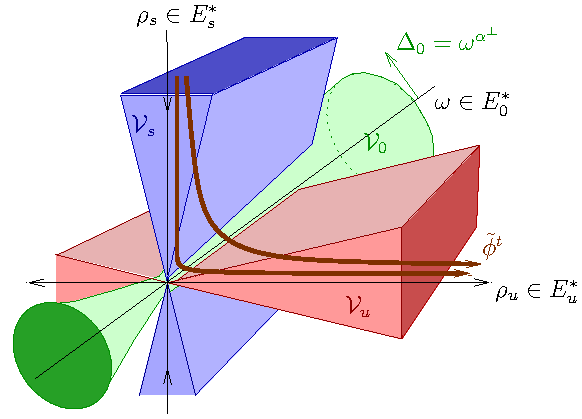
\includegraphics[scale=1]{zones_W1-1.pdf}
\vspace*{-10pt}
\caption{Representation of domains associated to the escape function $W_{2}$ defined in~\eqref{eq:def_W-1}: the domain \emph{$\clV_{s}$} in blue (respect. $\clV_{u}$ in red) is a conical neighborhood of $E_{s}^{*}$ (respect. of $E_{u}^{*}$) where the exponent is $a(\rho_{u}+\rho_{s})=\pm1$. Outside the domain $\clV_{0}:=\{ \rho;\,\langle \Vert \rho_{u}+\rho_{s}\Vert _{g_{\rho}}\rangle \asymp1\} =\{ \rho;\,|\rho_{u}+\rho_{s}|\apprle\omega^{\alpha^{\perp}}\} $ in green, the weight functions $W_{2}$ decays along the flow $\tilde{\phi}^{t}$.}
\label{fig:zones-1}
\vspace*{-10pt}
\end{figure}

We propose this escape function, because some escape function similar to $W_{2}$ has been constructed in~\cite{fred-roy-sjostrand-07} for Anosov diffeomorphisms and extended in~\cite{fred_flow_09} for Anosov flows. Later it has been used in the study of Ruelle resonances in different settings~\cite{dyatlov_Ruelle_resonances_2012,
dyatlov_faure_guillarmou_2014,dyatlov_guillarmou_2014,
dang_riviere_morse_smale_16,dyatlov_zworski_zeta_2013,
guillarmou_weich_resonances_16,jin_zworski_local_trace_14}. In particular this escape function $W_{2}$ is useful to construct space $\clH _{W}(M)$ that are fixed with respect to small perturbations of $X$, see~\cite{bonthonneau2018flow}. We could have use it in this paper, except for the proof of Theorem~\ref{thm:WF} that needs a parabolic neighborhood of $E_{u}^{*}$ and not only conical and for the proof of Theorem~\ref{thm:grey-band} that needs the decay controlled from below~\eqref{eq:decay_property-1}.

Let us consider the bundle $\bbP(\clE^{*})\rightarrow M$ where the fiber over $m\in M$ is the real projective space $\bbRP(\clE^{*}(m))$. Notice that $\tilde{\phi}^{t}:T^{*}M\rightarrow T^{*}M$ in~\eqref{eq:lifted_flow} induces a flow on $\bbP(\clE^{*})$ denoted by $\bbP\tilde{\phi}^{t}:\bbP(\clE^{*})\to\bbP(\clE^{*})$, because $\tilde{\phi}^{t}$ keeps the sub-bundle $\clE^{*}$ invariant and is linear in the fibers. For this flow $\bbP\tilde{\phi}^{t}$, the unstable direction $[E_{u}^{*}]\subset\bbP(\clE^{*})$ is an attractor and the stable direction $[E_{s}^{*}]\subset\bbP(\clE^{*})$ is a repeller. Let $a_{0}\in C^{\infty}(\bbP(\clE^{*});[-1,+1])$ be a smooth function such that
\begin{itemize}
\item $a_{0}\equiv-1$ on a vicinity $[\clV_{u}]\subset\bbP(\clE^{*})$ of the unstable direction $[E_{u}^{*}]\subset\bbP(\clE^{*})$ and
\item $a_{0}\equiv+1$ on a vicinity $[\clV_{s}]\subset\bbP(\clE^{*})$ of the stable direction $[E_{s}^{*}]\subset\bbP(\clE^{*})$.
\end{itemize}
From the function $a_{0}$ thus defined, we construct a smooth function $a\in C^{\infty}(\clE^{*};[-1,+1])$ by averaging it along finite orbits of $\bbP\tilde{\phi}^{t}$ as follows. Let $T>0$ be a constant and put
\begin{equation}\label{eq:def_a_T}
a\left(\rho_{*}\right)=\frac{1}{2T}\int_{-T}^{T}a_{0}\left(\bbP\tilde{\phi}^{t}\rho_{*}\right)dt
\end{equation}
for $\rho_{*}=\rho_{u}+\rho_{s}\in\clE^{*}$. In the next lemma, we will assume that $T>0$ is sufficiently large and denote by $\Vert v\Vert _{_{g(\rho)}}$ the norm of $v\in T_{\rho}(T^{*}M)$ with respect to the metric $g$ at $\rho\in T^{*}M$ defined in~\eqref{eq:def_norm_g}.

\begin{cBoxA}{}
\begin{defi}[Example~2 of a weight function $W_{2}$ with good properties]\label{lem:W1}
Assume that the parameters $\alpha^{\perp}$ and $\alpha^{\parallel}$ satisfy
\[
\frac{1}{1+\beta_{0}}\leq\alpha^{\perp}<1\quad\text{and}\quad0<\alpha^{\parallel}\leq\alpha^{\perp}.
\]
For $r>0$, we define the escape function $W_{2}:T^{*}M\rightarrow\bbR^{+}$ by
\begin{equation}\label{eq:def_W-1}
W_{2}\left(\rho\right):=\left\langle \left\Vert \rho_{u}+\rho_{s}\right\Vert _{g_{\rho}}\right\rangle ^{\frac{r}{\left(1-\alpha^{\perp}\right)}a\left(\rho_{u}+\rho_{s}\right)}
\end{equation}
where $\rho=\omega\scrA+\rho_{s}+\rho_{u}$ with $\omega\in\bbR$, $\rho_{u}\in E_{u}^{*}$, $\rho_{s}\in E_{s}^{*}$.
\end{defi}
\end{cBoxA}

\begin{cBoxB}{}
\begin{lemm}
The function $W_{2}$ in~\eqref{eq:def_W-1} has the following properties
\begin{enumerate}
\item \label{enu:-satisfies--temperate}
$W_{2}$ satisfies $h_{\gamma}^{\perp}$-temperate property~\eqref{eq:slow_variation_W} for any $0\leq\gamma<1$.
\item \label{enu:-satisfies-decay}
$W_{2}$ satisfies decay property~\eqref{eq:decay_property} with rate $\Lambda=\lambda_{\min}r$.
\item \label{enu:Its-order-is}
Its order is $r([\rho])=ra(\rho_{u}+\rho_{s})$ along $\clE_{*}$ in particular $r([\rho])=r$ along $E_{s}^{*}$ and $r([\rho])=-r$ along $E_{u}^{*}$.
\end{enumerate}
\end{lemm}
\end{cBoxB}

See Figure~\ref{fig:zones-1}. We can use the escape function $W_{2}$ to get Theorem~\ref{thm:Weyl law} about the density of eigenvalues. For this we choose the optimal values
\[
\alpha^{\perp}=\frac{1}{1+\beta_{0}},\quad\alpha^{\parallel}=0
\]
that give a transverse size $\Delta_{0}=\omega^{\frac{1}{1+\beta_{0}}}$ for the green region $\clV_{0}$ on Figure~\ref{fig:zones-1}.



\section{\label{sec:Hormander}
Relation with the class of symbols \texorpdfstring{$S_{\tilde{\rho},\tilde{\delta}}^{m}$}{S rho, deltam} of H\"ormander}

Let us give the relation between, on one side the metric $g$ on $T^{*}M$ with parameter $\alpha^{\perp}$, the conformal metric $g_{\gamma}=h_{\gamma}^{2}g$ with parameter $\gamma$ used in this paper and on the other side the (traditional) class of symbols $S_{\tilde{\rho},\tilde{\delta}}^{m}$ of H\"ormander~\cite[Chap.~18]{hormander_3} characterized by some parameters $m\in\bbR$, $0\leq\tilde{\delta}\leq\tilde{\rho}\leq1$, $\tilde{\delta}+\tilde{\rho}\geq1$. In this paper we have a metric in~\eqref{eq:metric_g_in_coordinates} similar to\footnote{The Weyl--H\"ormander calculus in principle enables to use metrics of a more general form than~\eqref{eq:g}, \cite{hormander1979weyl}.}
\begin{equation}\label{eq:g}
g:=\left(\frac{dx}{\delta^{\perp}\left(\xi\right)}\right)^{2}+\left(\delta^{\perp}\left(\xi\right)d\xi\right)^{2}
\end{equation}
on $(x,\xi)\in\bbR^{2n}$ (variable transverse to the flow direction) with
\begin{equation}\label{eq:delta_ex}
\delta^{\perp}\left(\xi\right)=\left\langle \left|\xi\right|\right\rangle ^{-\alpha^{\perp}}
\end{equation}
as defined in~\eqref{eq:def_delta} and parameter $\frac{1}{2}\leq\alpha^{\perp}<1$. We also have in~\eqref{eq:h_gamma}, a function of the form
\begin{equation}\label{eq:def_h-1}
h_{\gamma}\left(\xi\right):=\left\langle \left|\xi\right|\right\rangle ^{-\gamma},
\end{equation}
with $0\leq\gamma<1$. This function $h_{\gamma}(\xi)$ plays the role of a ``small Planck parameter'' and is associated to the re-scaled or conformal metric introduced by H\"ormander that is used to measure the variations of symbols on phase space~\cite{hormander1979weyl}, \cite[Chap.18]{hormander_3}, \cite[p.~22, p.~68]{lerner2011metrics},  \cite{nicola_rodino_livre_11}
\begin{align*}
g_{\gamma}\left(\xi\right) & {:=}\left(h_{\gamma}\left(\xi\right)\right)^{2}g\left(\xi\right)\\
& \!\!\underset{\eqref{eq:g}}{\asymp}\left(\frac{h_{\gamma}\left(\xi\right)dx}{\delta^{\perp}\left(\xi\right)}\right)^{2}+\left(h_{\gamma}\left(\xi\right)\delta^{\perp}\left(\xi\right)d\xi\right)^{2}\\
& \mkern-22mu\underset{\eqref{eq:delta_ex},\eqref{eq:def_h-1}}{=}\left(\frac{dx}{\left\langle \left|\xi\right|\right\rangle ^{-\tilde{\delta}}}\right)^{2}+\left(\frac{d\xi}{\left\langle \left|\xi\right|\right\rangle ^{\tilde{\rho}}}\right)^{2}
\end{align*}
with $\tilde{\delta}=\alpha^{\perp}-\gamma$ and $\tilde{\rho}=\alpha^{\perp}+\gamma$ that gives the relations
\begin{equation}\label{eq:relations-1}
\alpha^{\perp}:=\frac{1}{2}\left(\tilde{\rho}+\tilde{\delta}\right)\geq\frac{1}{2},\quad\gamma:=\frac{1}{2}\left(\tilde{\rho}-\tilde{\delta}\right)\geq0.
\end{equation}


\section{\label{sec:A-simple-model-of resonances}
How to reveal intrinsic discrete spectrum (resonances) on a simple model}

In this section we present an elementary model that explains why we observe discrete spectrum (resonances) in an appropriate Sobolev space though this is not the case for the usual $L^{2}$ space. At the end of the section, we will see the analogy between this simple model and the hyperbolic dynamics considered in this paper.

\subsection{The model}

Let us consider the following bi-infinite matrix $\clL=(\clL_{i,j})_{i,j\in\bbZ}$
\begin{equation}\label{eq:Matrix_L}
\clL:=\left(
\begin{array}{ccccc}
\ddots\\
\ddots & 0\\
& 1 & w_{0}\\
& & 1 & 0\\
0 & & -w_{1}^{-1} & 1 & \ddots
\end{array}\right)
\end{equation}
whose non-vanishing elements are only $\clL_{0,0}=w_{0}\in\bbC\backslash\{ 0\} $, $\clL_{2,0}=-w_{1}^{-1}\in\bbC$ and $\clL_{j+1,j}=1$ for every $j\in\bbZ$. Considering these non vanishing elements, we can associate to $\clL$ a ``Markov graph'' that contains the dynamics of a shift $\tilde{\phi}:j\mapsto j+1$, perturbed by a finite rank matrix, see Figure~\ref{fig:markov}.

\begin{figure}[h]
\centering
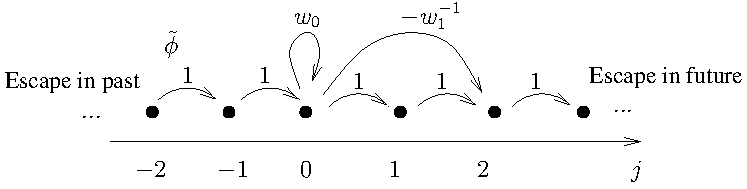
\includegraphics[scale=1]{figures/markov_full_shift-1.pdf} 
\caption{\label{fig:markov}
Markov graph associated to the infinite matrix~\eqref{eq:Matrix_L}.}
\end{figure}

\begin{rema}\label{rem:The-inverse-of}
The inverse matrix of $\clL$ is
\begin{equation}\label{eq:Matrix_L-1}
\clL^{-1}:=\left(
\begin{array}{ccccc}
\\
\ddots & 1 & & 0\\
& 0 & 1 & -w_{0}\\
& & 0 & 1\\
0 & & 0 & w_{1}^{-1} & \ddots\\
& & & & \ddots
\end{array}\right)
\end{equation}
where $(\clL^{-1})_{1,1}=w_{1}^{-1}$, $(\clL^{-1})_{-1,1}=-w_{0}$ and $(\clL^{-1})_{j,j+1}=1$ for $j\in\bbZ$. The matrix $\clL$ has the following eigenvectors $U$ and $V$:
\begin{itemize}
\item $\clL U=w_{0}U$ with vector $U=(\ldots,\,0,U_{0},\frac{1}{w_{0}}U_{0},\,\ldots,\,\frac{1}{w_{0}^{j}}(1-\frac{w_{0}}{w_{1}})U_{0},\,\ldots)\in\bbC^{\bbZ}$ with components $U_{j}=0$ for $j<0$, $U_{0}\in\bbC$, $U_{1}=\frac{1}{w_{0}}U_{0}$ and $U_{j}=\frac{1}{w_{0}^{j}}(1-\frac{w_{0}}{w_{1}})U_{0}$ for $j\geq2$. Hence $U\in l^{2}(\bbZ)$ if and only if $|w_{0}|>1$.
\item $\clL V=w_{1}V$ with vector $V=(\ldots,\,w_{1}^{1-j}(1-\frac{w_{0}}{w_{1}})V_{1},\,\ldots,\,w_{1}V_{1},V_{1},0,\,\ldots)\in\bbC^{\bbZ}$ with components $V_{1}\in\bbC$, $V_{0}=w_{1}V_{1}$, $V_{j}=w_{1}^{1-j}(1-\frac{w_{0}}{w_{1}})V_{1}$ for $j\leq-1$ and $V_{j}=0$ for $j\geq2$. Hence $V\in l^{2}(\bbZ)$ if and only if $|w_{1}|<1$.
\end{itemize}
\end{rema}

For some $r\in\bbR$ called the order, let us consider the following function $W$ on $\bbZ$,
\[
W\left(j\right):=e^{-rj},\quad j\in\bbZ.
\]
For $j\neq0,2$ we have $\frac{W(\tilde{\phi}(j))}{W(j)}=e^{-r}$ hence if $r>0$, $W$ decreases along the trajectories of $\tilde{\phi}$ and we call $W$ an ``escape function''. Let $\Diag(W)$ be the diagonal matrix with diagonal elements $W(j)$. Let
\begin{align}\label{eq:def_L_tilde_W}
\tilde{\clL}_{W}: & =\Diag\left(W\right)\circ\clL\circ\Diag\left(W\right)^{-1}\underset{\eqref{eq:Matrix_L}}{=}\left(
\begin{array}{ccccc}
\\
\ddots & 0 & & 0\\
& e^{-r} & w_{0}\\
& & e^{-r} & 0\\
0 & & -e^{-2r}w_{1}^{-1} & e^{-r} & \ddots\\
& & & & \ddots
\end{array}\right)
\end{align}
We refer to~\cite[Chap.~1]{bottcher2012introduction}, \cite[p.~51]{trefethen_book_05} for the spectrum of Toeplitz operators.

\begin{lemm}\label{lem:spectrum}
The operator $\tilde{\clL}_{W}:l^{2}(\bbZ)\rightarrow l^{2}(\bbZ)$ has essential spectrum on the circle of radius $e^{-r}$ and the following discrete spectrum elsewhere: $w_{0}$ is an eigenvalue if and only if $|w_{0}|>e^{-r}$. $w_{1}$ is an eigenvalue if and only if $|w_{1}|<e^{-r}$.
\end{lemm}

We define
\[
\clH _{W}\left(\bbZ\right):=\Diag\left(W\right)^{-1}\left(l^{2}\left(\bbZ\right)\right)
\]
meaning that the norm of a vector $u\in\clH _{W}(\bbZ)$ is
\begin{equation}\label{eq:norm_W}
\left\Vert u\right\Vert _{\clH _{W}\left(\bbZ\right)}^{2}:=\left\Vert \Diag\left(W\right)u\right\Vert _{l^{2}\left(\bbZ\right)}^{2}=\sum_{j\,\in\,\bbZ}\left|e^{-rj}u_{j}\right|^{2}
\end{equation}
$\clH _{W}(\bbZ)$ is similar to a anisotropic Sobolev space with weight $W(j)=e^{-rj}$. We have the following commutative diagram
\[
\begin{CD}\clH _{W}\left(\bbZ\right)@>{\clL}>>\clH _{W}\left(\bbZ\right)\\
@V{\Diag\left(W\right)}VV@V{\Diag\left(W\right)}VV\\
l^{2}\left(\bbZ\right)@>{\tilde{\clL}_{W}:=\Diag\left(W\right)\circ\clL\circ\Diag\left(W\right)^{-1}}>>l^{2}\left(\bbZ\right)
\end{CD}
\]
%Revoir la forme utiliser des xymatrix!
\noindent where $\Diag(W):\clH _{W}(\bbZ)\rightarrow l^{2}(\bbZ)$ is an isometry (by definition) and hence Lemma~\ref{lem:spectrum} gives
\begin{lem}
The operator $\clL:\clH _{W}(\bbZ)\rightarrow\clH _{W}(\bbZ)$ has essential spectrum on the circle of radius $e^{-r}$ and the following discrete spectrum elsewhere: $w_{0}$ is an eigenvalue with eigenvector $U\in\clH _{W}(\bbZ)$ if and only if $|w_{0}|>e^{-r}$. $w_{1}$ is an eigenvalue with eigenvector $V\in\clH _{W}(\bbZ)$ if and only $|w_{1}|<e^{-r}$.
\end{lem}

See Figure~\ref{fig:spectrum_matrix}.

\begin{figure}[!htbp]
\centering
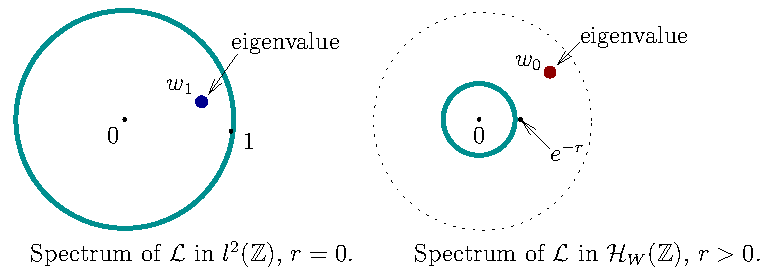
\includegraphics{spectrum_matrix-1.pdf}
\caption{In this picture we assume $|w_{0}|=|w_{1}|<1$. The circle of radius $e^{-r}$ (in green) is the essential spectrum of $\clL$ in the space $\clH _{W}(\bbZ)$ that depends on $r\in\bbR$. As $r\rightarrow+\infty$ this circle shrinks to zero and we reveal the intrinsic ``future discrete spectrum'' of $\clL$, here this is the eigenvalue $w_{0}$ (in red), as soon as $e^{-r}<|w_{0}|$. As $r\rightarrow-\infty$ this circle goes to infinity and we reveal the intrinsic ``past discrete spectrum'' of $\clL$, here this is the eigenvalue $w_{1}$ (in blue), as soon as $|w_{1}|<e^{-r}$.}
\label{fig:spectrum_matrix}
\end{figure}


\paragraph{The conclusion of this simple model is that:}
\begin{enumerate}
\item We observe that the given matrix $\clL$ corresponds to a simple dynamics $\tilde{\phi}$ and outside a compact region, the dynamics of $\tilde{\phi}$ escapes to/from infinity.
\item We construct an ``escape function'' $W$ for that dynamic $\tilde{\phi}$ that decays with rate $e^{-r}$ and define an anisotropic Sobolev space $\clH _{W}(\bbZ):=\Diag(W)^{-1}(l^{2}(\bbZ))$.
\item It appears that the matrix $\clL$ has essential spectral radius $r_{\esss}=e^{-r}$ in $\clH _{W}(\bbZ)$. Moreover, by increasing the parameter $r$ we get $r_{\esss}=e^{-r}\underset{r\,\rightarrow\,+\infty}{\rightarrow0}$ and this may reveal new eigenvalues and eigenspaces of $\clL$ that do not depend on $W$ (here we have only $w_{0}\in\bbC$) that we call ``future discrete spectrum''. If we do $r_{\esss}=e^{-r}\underset{r\,\rightarrow\,-\infty}{\rightarrow+\infty}$ this may reveal new eigenvalues and eigenspaces of $\clL$ that do not depend on $W$ (here we have only $w_{1}\in\bbC$) that we call ``past discrete spectrum''. The past discrete spectrum is the future discrete spectrum for $\clL^{-1}$ and conversely. See Figure~\ref{fig:spectrum_matrix}.
\end{enumerate}
\begin{rema}
For $j\neq0$, the dynamics $\tilde{\phi}:j\mapsto j+1$ is a translation. Observe that
\begin{itemize}
\item For $j>0$, if we set $\xi_{u}:=e^{j}$, we get an expanding dynamics $\tilde{\phi}:\xi_{u}\mapsto e^{1}\xi_{u}$. The escape function is $W(j)=e^{-jr}=\xi_{u}^{-r}$ hence the anisotropic Sobolev space $\clH _{W}(\bbZ)$ has negative order $-r$.
\item For $j<0$, if we set $\xi_{s}:=e^{-j}$, we get a contracting dynamics $\tilde{\phi}:\xi_{s}\mapsto e^{-1}\xi_{s}$. The escape function is $W(j)=e^{-jr}=\xi_{s}^{r}$ hence the anisotropic Sobolev space $\clH _{W}(\bbZ)$ has positive order $r$.
\end{itemize}
The fact that the order depends on the sign of $j$ explains the term ``anisotropic''.
\end{rema}


\begin{rema}
Starting from the semi infinite matrix
\[
\clL:=\
\begin{pmatrix}
w_{0} & & & 0\\
1 & 0\\
& 1 & 0\\
0 & & \ddots & \ddots
\end{pmatrix}
\]
we would have a similar analysis with the difference that the dynamics is $\tilde{\phi}(j)=j+1$ is a semi-shift and the spectrum in $\clH _{W}(\bbN)$ is essential on the circle of radius $e^{-r}$ and residual inside. If one chooses the escape function $W(j)=e^{-j^{\alpha}}=e^{-(\log\xi)^{\alpha}}$ with some $\alpha>1$, we get that $\frac{W(j+1)}{W(j)}\rightarrow0$ as $j\rightarrow\infty$ and that $\clL$ is Trace class in $\clH _{W}(\bbZ)$ with Trace obtained as the sum over the discrete spectrum (the essential spectrum has shrunk to $0$ immediately). This model corresponds to the so-called Gevrey class in $\xi$ variable (and their dual). Even stronger, if one choose the escape function $W\left(j\right)=e^{-re^{j}}=e^{-r\xi}$ with some $r>0$, we get that $\frac{W(j+1)}{W(j)}=e^{-r(e-1)e^{j}}\rightarrow0$ as $j\rightarrow\infty$. This model corresponds to ``analytic class'' in $\xi$ variable (and their dual of hyper-functions).
\end{rema}


\begin{rema}
We can replace the single element $w_{0}\in\bbC$ on the diagonal of $\clL$ by a finite rank (or compact) matrix with eigenvalues $w_{0},w_{1},\,\ldots$. From the discrete spectrum of $\clL$ in $\clH _{W}(\bbZ)$, we deduce decay of correlations for $u,v\in\clH _{W}(\bbZ)$:
\[
\left\langle u\,\middle|\,\clL^{t}v\right\rangle_{\clH _{W}\left(\bbZ\right)}=\sum_{k}w_{k}^{t}\left\langle u\,\middle|\,\clL^{t}\pi_{k}v\right\rangle_{\clH _{W}\left(\bbZ\right)}+O\left(e^{-\lambda rt}\right)\underset{t\,\rightarrow\,+\infty}{\sim}w_{0}^{t}\left\langle u\,\middle|\,\clL^{t}\pi_{0}v\right\rangle
\]
where $\pi_{k}$ is the spectral projector associated to the eigenvalue $w_{k}$ and we have assumed that $|w_{0}|>|w_{j}|$ for $j\geq1$.
\end{rema}


\subsection{Analogy with Ruelle resonances for hyperbolic dynamics}

In the table on next page we put in correspondence the properties of the matrix $\clL$, \eqref{eq:Matrix_L} and the transfer operator $\clL^{t}=e^{tA}$ studied in this paper that is defined from an Anosov flow $\phi^{t}$ on $M$.
%%Regarder si il est possible de mettre 2,5pt d'espace entre la ligne et le contenu de la cellule.
\begin{table}
\centering
\begin{tabular}{|l|l|}
\hline Matrix model $\clL$ & Hyperbolic dynamics\tabularnewline
\hline
\hline Orthonormal basis & Almost orthogonal basis of wave-packets\tabularnewline $\varphi_{j}=\left(0\ldots,\,\underset{(j)}{1},0\ldots\right)\in l^{2}\left(\bbZ\right)$, $j\in\bbZ$. & {$\varphi_{\rho}\in L^{2}\left(M\right)$, }with $\rho\in T^{*}M$.\tabularnewline
\hline The action of $\clL$ is described by & The action of $\clL^{t}$ is described by\tabularnewline a dynamics $\tilde{\phi}$ on $\bbZ$, & the lifted flow $\tilde{\phi}$ on $\rho=\left(x,\xi\right)\in T^{*}M$,\tabularnewline hyperbolic in $\xi_{u},\xi_{s}=e^{\pm j}$ & hyperbolic in $\xi$.\tabularnewline
\hline Escape function $W\left(j\right)$, & Escape function $W$ on $T^{*}M$\tabularnewline with decay property $\frac{W\left(\tilde{\phi}\left(j\right)\right)}{W\left(j\right)}=e^{-r}$. & with temperate and decay property\tabularnewline & $\frac{W\left(\tilde{\phi}^{t}\left(\rho\right)\right)}{W\left(\rho\right)}\leq Ce^{-\Lambda t}$ outside the trapped set $E_{0}^{*}$.\tabularnewline
\hline $\clH _{W}\left(\bbZ\right):=\Diag\left(W\right)^{-1}\left(l^{2}\left(\bbZ\right)\right)$ & $\clH _{W}\left(M\right):=\Opp \left(W\right)^{-1}\left(L^{2}\left(M\right)\right)$\tabularnewline & with $\Opp \left(W\right)$ a PDO.\tabularnewline & i.e. almost diagonal in wave-packet basis.\tabularnewline
\hline $\clS_{\xi}\subset\clH _{W}\left(\bbZ\right)\subset\clS_{\xi}'$ & $\clS\left(M\right)\subset\clH _{W}\left(M\right)\subset\clS'\left(M\right)$\tabularnewline
\hline Discrete spectrum $w=e^{z}$ on & Discrete spectrum $z$ of the generator $A$\tabularnewline $\left|w\right|>e^{-1.r}\Leftrightarrow\Ree\left(z\right)>-1.r$. & on $\Ree\left(z\right)>-\lambda_{\min}r+\Cste$.\tabularnewline
\hline
\end{tabular}
\end{table}

\section{Relations for the Japanese bracket \texorpdfstring{$\left\langle.\right\rangle $}{<.> }}

For $s\in\bbR$, we set
\[
\langle s\rangle:=(1+s^{2})^{1/2}.
\]
Clearly we have
\[
\max\{1,|s|\}\le\langle s\rangle\le\langle\langle s\rangle\rangle\le2\max\{1,|s|\}
\]
and
\[
\frac{d}{ds}\langle s\rangle=\frac{s}{\sqrt{1+s^{2}}}\in(-1,1)\quad\text{for any \ensuremath{s\in\bbR}.}
\]
From the second estimate, it follows
\begin{equation}\label{eq:sum}
\langle s+t\rangle\le\langle s\rangle+|t|\le\langle s\rangle+\langle t\rangle
\end{equation}
that implies
\begin{equation}\label{eq:D1p}
\frac{\left\langle t\right\rangle }{\left\langle s\right\rangle }\leq1+\frac{\left|t-s\right|}{\left\langle s\right\rangle }\leq1+\left|t-s\right|
\end{equation}

Also, by considering the cases $|s|\le1$ and $|s|>1$ separately, we can check
\begin{equation}\label{eq:prod}
\langle s\cdot t\rangle\le\max\{1,|s|\}\cdot\langle t\rangle\le\langle s\rangle\cdot\langle t\rangle
\end{equation}
Note that~\eqref{eq:prod} implies that, if $s\neq0$,
\[
\langle t\rangle=\left\langle s\cdot s^{-1}t\right\rangle\le\max\{1,|s|\}\cdot\left\langle s^{-1}t\right\rangle
\]
and hence
\begin{equation}\label{eq:prod2}
\left\langle\frac{t}{s}\right\rangle\ge\max\{1,|s|\}^{-1}\langle t\rangle\ge\frac{\left\langle t\right\rangle }{\left\langle s\right\rangle}.
\end{equation}




\begin{thebibliography}{99}
\bibitem{https://doi.org/10.48550/arxiv.1809.04062}Adam, Alexander; Baladi, Viviane Horocycle averages on closed manifolds and transfer operators, Tunis. J. Math., Volume 4 (2022) no. 3, pp. 387-441 | Zbl | DOI | MR
\bibitem{Baladi05}Baladi, Viviane Anisotropic Sobolev spaces and dynamical transfer operators: ${C}^\infty $ foliations, Algebraic and topological dynamics (Contemporary Mathematics), Volume 385, American Mathematical Society, 2005, pp. 123-135 | Zbl | DOI | MR
\bibitem{bonthonneau2020fbi}Bonthonneau, Yannick Guedes; Jézéquel, Malo FBI Transform in Gevrey classes and Anosov flows (2020) (https://arxiv.org/abs/2001.03610)
\bibitem{liverani_02}Blank, Michael; Keller, Gerhard; Liverani, Carlangelo Ruelle–Perron–Frobenius spectrum for Anosov maps, Nonlinearity, Volume 15 (2002) no. 6, pp. 1905-1973 | Zbl | DOI | MR
\bibitem{liverani_butterley_07}Butterley, Oliver; Liverani, Carlangelo Smooth Anosov flows: correlation spectra and stability, J. Mod. Dyn., Volume 1 (2007) no. 2, pp. 301-322 | Zbl | DOI | MR
\bibitem{bonthonneau2018flow}Bonthonneau, Yannick Guedes Flow-independent Anisotropic space, and perturbation of resonances, Rev. Unión Mat. Argent., Volume 61 (2020) no. 1, pp. 63-72 | DOI | Zbl | MR
\bibitem{bottcher2012introduction}Böttcher, Albrecht; Silbermann, Bernd Introduction to large truncated Toeplitz matrices, Universitext, Springer, 2012 | Zbl
\bibitem{baladi_05}Baladi, Viviane; Tsujii, Masato Anisotropic Hölder and Sobolev spaces for hyperbolic diffeomorphisms, Ann. Inst. Fourier, Volume 57 (2007) no. 1, pp. 127-154 | Zbl | DOI | Numdam
\bibitem{da_silva_01}Cannas Da Silva, Ana Lectures on Symplectic Geometry, Lecture Notes in Mathematics, 1764, Springer, 2001 | Zbl | MR
\bibitem{dyatlov_Ruelle_resonances_2012}Datchev, Kiril; Dyatlov, Semyon; Zworski, Maciej Sharp polynomial bounds on the number of Pollicott-Ruelle resonances, Ergodic Theory Dyn. Syst. (2012), pp. 1-16 | Zbl
\bibitem{dyatlov_faure_guillarmou_2014}Dyatlov, Semyon; Faure, Frédéric; Guillarmou, Colin Power spectrum of the geodesic flow on hyperbolic manifolds, Anal. PDE, Volume 8 (2015) no. 4, pp. 923-1000 | Zbl | DOI | MR
\bibitem{dyatlov_guillarmou_2014}Dyatlov, Semyon; Guillarmou, Colin Pollicott–Ruelle resonances for open systems, Ann. Henri Poincaré, Volume 17 (2016) no. 11, pp. 3089-3146 | DOI | Zbl | MR
\bibitem{dang_riviere_morse_smale_16}Dang, Nguyen Viet; Riviere, Gabriel Spectral analysis of Morse–Smale gradient flows, Ann. Sci. Éc. Norm. Supér., Volume 52 (2019) no. 6, pp. 1403-1458 | DOI | Zbl | MR
\bibitem{dyatlov_2021_pollicott_ruelle_sobolev}Dyatlov, Semyon Pollicott–Ruelle resolvent and Sobolev regularity, Pure Appl. Funct. Anal., Volume 8 (2023) no. 1, pp. 187-213 | DOI | MR | Zbl
\bibitem{dyatlov_zworski_zeta_2013}Dyatlov, Semyon; Zworski, Maciej Dynamical zeta functions for Anosov flows via microlocal analysis, Ann. Sci. Éc. Norm. Supér., Volume 49 (2016) no. 3, pp. 543-577 | Zbl | DOI | MR
\bibitem{engel_1999}Engel, Klaus-Jochen; Nagel, Rainer One-parameter semigroups for linear evolution equations, Graduate Texts in Mathematics, 194, Springer, 1999 | Zbl
\bibitem{falconer_03_book}Falconer, Kenneth J. Fractal geometry: mathematical foundations and applications, John Wiley \& Sons, 2003 | Zbl | DOI
\bibitem{folland-88}Folland, Gerald B. Harmonic Analysis in phase space, Annals of Mathematics Studies, 122, Princeton University Press, 1989 | Zbl | DOI
\bibitem{fred-RP-06}Faure, Frédéric; Roy, Nicolas Ruelle–Pollicott resonances for real analytic hyperbolic map, Nonlinearity, Volume 19 (2006) no. 6, pp. 1233-1252 | DOI | Zbl | MR
\bibitem{fred-roy-sjostrand-07}Faure, Frédéric; Roy, Nicolas; Sjöstrand, Johannes A semiclassical approach for Anosov Diffeomorphisms and Ruelle resonances, Open Math. J., Volume 1 (2008), pp. 35-81 | Zbl | DOI
\bibitem{fred_flow_09}Faure, Frédéric; Sjöstrand, Johannes Upper bound on the density of Ruelle resonances for Anosov flows. A semiclassical approach, Commun. Math. Phys., Volume 308 (2011) no. 2, pp. 325-364 | DOI | Zbl
\bibitem{faure_tsujii_band_CRAS_2013}Faure, Frédéric; Tsujii, Masato Band structure of the Ruelle spectrum of contact Anosov flows, C. R. Math. Acad. Sci. Paris, Volume 351 (2013) no. 9-10, pp. 385-391 | DOI | Zbl | MR | Numdam
\bibitem{faure-tsujii_prequantum_maps_12}Faure, Frédéric; Tsujii, Masato Prequantum transfer operator for symplectic Anosov diffeomorphism, Astérisque, 375, Société Mathématique de France, 2015 | Zbl
\bibitem{faure-tsujii_anosov_flows_13}Faure, Frédéric; Tsujii, Masato The semiclassical zeta function for geodesic flows on negatively curved manifolds, Invent. Math., Volume 208 (2017) no. 3, pp. 851-998 | DOI | Zbl | MR
\bibitem{faure-tsujii_anosov_flows_16}Faure, Frédéric; Tsujii, Masato Microlocal analysis and Band structure of contact Anosov flows (2021) (https://arxiv.org/abs/2102.11196v1)
\bibitem{guillarmou_weich_resonances_16}Guillarmou, Colin; Hilgert, Joachim; Weich, Tobias Classical and quantum resonances for hyperbolic surfaces, Math. Ann., Volume 370 (2018) no. 3-4, pp. 1231-1275 | DOI | Zbl | MR
\bibitem{liverani_04}Gouëzel, Sébastien; Liverani, Carlangelo Banach spaces adapted to Anosov systems, Ergodic Theory Dyn. Syst., Volume 26 (2005) no. 1, pp. 189-217 | Zbl | DOI | MR
\bibitem{grigis_sjostrand}Grigis, Alain; Sjöstrand, Johannes Microlocal analysis for differential operators. An introduction, London Mathematical Society Lecture Note Series, 196, Cambridge University Press, 1994 | Zbl | DOI
\bibitem{hasselblatt1994regularity}Hasselblatt, Boris Regularity of the Anosov splitting and of horospheric foliations, Ergodic Theory Dyn. Syst., Volume 14 (1994) no. 4, pp. 645-666 | DOI | Zbl | MR
\bibitem{hurder-90}Hurder, Steven E.; Katok, Anatole Differentiability, rigidity and Godbillon-Vey classes for Anosov flows, Publ. Math., Inst. Hautes Étud. Sci., Volume 72 (1990), pp. 5-61 | Zbl | DOI | Numdam
\bibitem{sjostrand_87}Helffer, Bernard; Sjöstrand, Johannes Résonances en limite semi-classique. (Resonances in semi-classical limit), Mémoires de la Société Mathématique de France. Nouvelle Série, 24/25, Société Mathématique de France, 1986 | Zbl
\bibitem{sjostrand_hitrick_07}Hitrik, Michael; Sjöstrand, Johannes Rational invariant tori, phase space tunneling, and spectra for non-selfadjoint operators in dimension 2, Ann. Sci. Éc. Norm. Supér., Volume 41 (2008) no. 4, pp. 513-573 | DOI | Zbl | MR | Numdam
\bibitem{hormander1979weyl}Hörmander, Lars The Weyl calculus of pseudo-differential operators, Commun. Pure Appl. Math., Volume 32 (1979) no. 3, pp. 359-443 | DOI | Zbl
\bibitem{hormander_3}Hörmander, Lars The analysis of linear partial differential operators. II: Differential operators with constant coefficients, Grundlehren der Mathematischen Wissenschaften, 257, Springer, 1983 | Zbl
\bibitem{hormander_1}Hörmander, Lars The Analysis of the Linear Partial Differential Operators I: Distribution Theory and Fourier Analysis. Classics in Mathematics, Classics in Mathematics, Springer, 2003 (reprint of the 2nd edition 1990) | Zbl | DOI
\bibitem{jenkinson_2018}Jenkinson, Oliver Ergodic optimization in dynamical systems, Ergodic Theory Dyn. Syst. (2018), pp. 1-26 | DOI | Zbl
\bibitem{jin_zworski_local_trace_14}Jin, Long; Zworski, Maciej A local trace formula for Anosov flows, Ann. Henri Poincaré, Volume 18 (2017) no. 1, pp. 1-35 | Zbl | MR
\bibitem{jezequel2020spectral_thesis}Jézéquel, Malo Spectral theory for ultradifferentiable hyperbolic dynamics, Ph. D. Thesis, Sorbonne-Université, Paris, France (2020)
\bibitem{lerner2011metrics}Lerner, Nicolas Metrics on the phase space and non-selfadjoint pseudo-differential operators, Pseudo-Differential Operators. Theory and Applications, 3, Springer, 2011 | Zbl | Numdam
\bibitem{martinez-01}Martinez, André An Introduction to Semiclassical and Microlocal Analysis, Universitext, Springer, 2002 | Zbl | DOI
\bibitem{https://doi.org/10.48550/arxiv.2107.08875}Meddane, Antoine A Morse complex for Axiom A flows (2021) (https://arxiv.org/abs/2107.08875) | DOI
\bibitem{mac_duff_98}McDuff, Dusa; Salamon, Dietmar Introduction to symplectic topology. 2nd edition, Oxford Mathematical Monographs, Clarendon Press, 1998 | Zbl
\bibitem{nicola_rodino_livre_11}Nicola, Fabio; Rodino, Luigi Global pseudo-differential calculus on Euclidean spaces, Pseudo-Differential Operators. Theory and Applications, 4, Springer, 2011 | Zbl
\bibitem{Nonnenmacher_Zworski_14}Nonnenmacher, Stéphane; Sjöstrand, Johannes; Zworski, Maciej Fractal Weyl law for open quantum chaotic maps, Ann. Math., Volume 179 (2014) no. 1, pp. 179-251 | DOI | Zbl | MR
\bibitem{pazy_semigroups_83}Pazy, André Semigroups of linear operators and applications to partial differential equations, 44, Springer, 1983 | Zbl | DOI
\bibitem{sjostrand_90}Sjöstrand, Johannes Geometric bounds on the density of resonances for semiclassical problems, Duke Math. J., Volume 60 (1990) no. 1, pp. 1-57 | MR | Zbl
\bibitem{sjostrand_density_resonances_96}Sjöstrand, Johannes Density of resonances for strictly convex analytic obstacles, Can. J. Math., Volume 48 (1996) no. 2, pp. 397-447 (with an appendix by M. Zworski) | MR | Zbl | DOI
\bibitem{sjostrand_2000}Sjöstrand, Johannes Asymptotic distribution of eigenfrequencies for damped wave equations, Publ. Res. Inst. Math. Sci., Volume 36 (2000) no. 5, pp. 573-611 | Zbl | DOI | MR | Numdam
\bibitem{taylor_tome1}Taylor, Michael E. Partial differential equations. Vol. I: Basic theory, Applied Mathematical Sciences, 115, Springer, 1996 | Zbl
\bibitem{taylor_tome2}Taylor, Michael E. Partial differential equations. Vol. II: Qualitative studies of linear equations, Applied Mathematical Sciences, 116, Springer, 1996 | Zbl | DOI
\bibitem{trefethen_book_05}Trefethen, Lloyd N.; Embree, Mark Spectra and pseudospectra. The behavior of nonnormal matrices and operators, Princeton University Press, 2005 | Zbl | DOI
\bibitem{tsujii_08}Tsujii, Masato Quasi-compactness of transfer operators for contact Anosov flows, Nonlinearity, Volume 23 (2010) no. 7, pp. 1495-1545 | Zbl | DOI | MR
\bibitem{tsujii_FBI_10}Tsujii, Masato Contact Anosov flows and the Fourier–Bros–Iagolnitzer transform, Ergodic Theory Dyn. Syst., Volume 32 (2012) no. 6, pp. 2083-2118 | Zbl | DOI | MR
\bibitem{wunsh-zworski_01}Wunsch, Jared; Zworski, Maciej The FBI transform on compact $\mathcal{C}^\infty $ manifolds., Trans. Am. Math. Soc., Volume 353 (2001) no. 3, pp. 1151-1167 | Zbl | DOI | MR
\bibitem{zworski_book_2012}Zworski, Maciej Semiclassical Analysis, Graduate Studies in Mathematics, 138, American Mathematical Society, 2012 | Zbl | DOI
\end{thebibliography}
\end{document}
